\documentclass[
  ngerman,english, % change to ngerman for german theses
  BCOR=0mm,cdgeometry=no,DIV=13, % use two-side for booklike layouts
  numbers=noenddot, % remove trailing dots in chapter/section/... enumeration
  cd=fullcolor,
  headings=heavy,
  chapterpage=true,
  cdfont=off, % modify this to use the TUD font (Open Sans)
  egregdoesnotlikesansseriftitles
]{tudscrmanual}

% use a custom serif font
\usepackage[bitstream-charter]{mathdesign}

\usepackage[hyphens]{url}

\usepackage[T1]{fontenc}
\usepackage[utf8]{inputenc}
\usepackage[
  english % change to ngerman for german theses
]{babel}
\usepackage{isodate}
\usepackage{pdfpages}
\usepackage{listings}
\usepackage[toc, page]{appendix}
\usepackage{hyphenat}

\usepackage[
  style=ieee,
  backend=biber,
  url=false,
  doi=false,
  isbn=false,
  hyperref,
]{biblatex}
% configure the location of the biblatex file
\addbibresource{students.bib}
\addbibresource{papers.bib}
\addbibresource{bibliography.bib}
\AtEveryBibitem{%
  \clearfield{note}%
}

\usepackage{graphicx}
\graphicspath{ {./} }
\usepackage{svg}

\usepackage{caption}
\captionsetup{font={footnotesize},labelsep=colon,justification=centering,format=plain}
\usepackage{floatrow}
\floatsetup{font=normalfont}
\floatsetup[table]{style=plaintop}
\DeclareCaptionSubType[alph]{figure}
\DeclareCaptionSubType[alph]{table}

\usepackage{booktabs}
\usepackage{longtable}

\usepackage{enumitem}
\setlist[itemize]{noitemsep}
\setlist{parsep=0pt,listparindent=\parindent}

\usepackage{float}
\usepackage{pgf}

% configure the name of your appendix
\renewcommand\appendixtocname{Appendix}
\renewcommand\appendixpagename{Appendix}

% use \tocless before a chapter/section/... in the
% appendix to hide it from the toc
\newcommand{\nocontentsline}[3]{}
\newcommand{\tocless}[2]{
  \bgroup\let\addcontentsline=\nocontentsline#1{#2}\egroup
}

\usepackage{amsmath}

% https://github.com/priobike/priobike-flutter-app/blob/dev/lib/common/layout/ci.dart
\definecolor{ciblue}{HTML}{0073ff}
\definecolor{cidarkblue}{HTML}{003064}
\usepackage[colorlinks=true,allcolors=ciblue]{hyperref}%
\usepackage[capitalise,nameinlink,noabbrev]{cleveref} % Must be loaded after amsmath
\hypersetup{
  colorlinks=true,
  linkcolor=black,
  filecolor=ciblue,
  citecolor=ciblue,      
  urlcolor=ciblue,
}

\usepackage{listings}
\definecolor{background}{HTML}{F6F6FE}
\usepackage[scaled=0.85]{beramono}
\lstdefinelanguage{python}{
    basicstyle=\ttfamily\footnotesize,
    numbers=left,
    numberstyle=\scriptsize,
    stepnumber=1,
    numbersep=8pt,
    showstringspaces=false,
    breaklines=true,
    frame=lines,
    backgroundcolor=\color{background},
    literate=
     *{0}{{{\color{cidarkblue}0}}}{1}
      {1}{{{\color{cidarkblue}1}}}{1}
      {2}{{{\color{cidarkblue}2}}}{1}
      {3}{{{\color{cidarkblue}3}}}{1}
      {4}{{{\color{cidarkblue}4}}}{1}
      {5}{{{\color{cidarkblue}5}}}{1}
      {6}{{{\color{cidarkblue}6}}}{1}
      {7}{{{\color{cidarkblue}7}}}{1}
      {8}{{{\color{cidarkblue}8}}}{1}
      {9}{{{\color{cidarkblue}9}}}{1}
      {:}{{{\color{cidarkblue}{:}}}}{1}
      {,}{{{\color{cidarkblue}{,}}}}{1}
      {\{}{{{\color{cidarkblue}{\{}}}}{1}
      {\}}{{{\color{cidarkblue}{\}}}}}{1}
      {[}{{{\color{cidarkblue}{[}}}}{1}
      {]}{{{\color{cidarkblue}{]}}}}{1},
}

\usepackage[framemethod=tikz]{mdframed}
\newcounter{Summary}[section]
\newenvironment{Summary}[1][]{%
\stepcounter{Summary}%
\ifstrempty{#1}%
{\mdfsetup{%
frametitle={%
\tikz[baseline=(current bounding box.east)]
% Theorem
\node[anchor=east,rectangle,fill=blue!20]
{\strut};}}
}%
{\mdfsetup{%
frametitle={%
{\strut \color{cidarkblue}\textrm{#1}}}}%
}%
\mdfsetup{innertopmargin=0pt,innerbottommargin=0pt,innerrightmargin=16pt,innerleftmargin=0pt,linecolor=cidarkblue,linewidth=2pt,topline=false,bottomline=false,leftline=false,}
\begin{mdframed}[]\relax%
}{\end{mdframed}}

% use this custom theorem for research questions
\newtheorem{researchquestion}{Research Question}
\crefname{researchquestion}{Research Question}{Research Questions}

\renewcommand{\floatpagefraction}{.8}% Avoid pages that only contain one image, but no text
\usepackage[all]{nowidow}% Avoid orphaned lines on new pages

\setlength{\parindent}{0cm}
\setlength{\parskip}{0.3cm plus 1mm minus 1mm}
\setlength{\intextsep}{0.6cm}

\begin{document}
\addtokomafont{disposition}{\rmfamily}
\addtokomafont{title}{\rmfamily}
\addtokomafont{titlepage}{\rmfamily}
\addtokomafont{thesis}{\rmfamily}
\addtokomafont{tudheadings}{\rmfamily}
\addtokomafont{partsubtitle}{\rmfamily}
\addtokomafont{chaptersubtitle}{\rmfamily}
\addtokomafont{author}{\rmfamily}
\addtokomafont{caption}{\rmfamily}
\addtokomafont{captionlabel}{\rmfamily}
\addtokomafont{chapter}{\rmfamily}
\addtokomafont{chapterentry}{\rmfamily}
\addtokomafont{chapterentrydots}{\rmfamily}
\addtokomafont{chapterentrypagenumber}{\rmfamily}
\addtokomafont{chapterprefix}{\rmfamily}
\addtokomafont{date}{\rmfamily}
\addtokomafont{dedication}{\rmfamily}
\addtokomafont{descriptionlabel}{\rmfamily}
\addtokomafont{dictum}{\rmfamily}
\addtokomafont{dictumtext}{\rmfamily}
\addtokomafont{footnote}{\rmfamily}
\addtokomafont{footnotelabel}{\rmfamily}
\addtokomafont{footnotereference}{\rmfamily}
\addtokomafont{footnoterule}{\rmfamily}
\addtokomafont{labelinglabel}{\rmfamily}
\addtokomafont{labelingseparator}{\rmfamily}
\addtokomafont{minisec}{\rmfamily}
\addtokomafont{pagefoot}{\rmfamily}
\addtokomafont{pagehead}{\rmfamily}
\addtokomafont{pageheadfoot}{\rmfamily}
\addtokomafont{pagenumber}{\rmfamily}
\addtokomafont{pagination}{\rmfamily}
\addtokomafont{paragraph}{\rmfamily}
\addtokomafont{part}{\rmfamily}
\addtokomafont{partentry}{\rmfamily}
\addtokomafont{partentrypagenumber}{\rmfamily}
\addtokomafont{partnumber}{\rmfamily}
\addtokomafont{publishers}{\rmfamily}
\addtokomafont{section}{\rmfamily}
\addtokomafont{sectioning}{\rmfamily}
\addtokomafont{subject}{\rmfamily}
\addtokomafont{subparagraph}{\rmfamily}
\addtokomafont{subsection}{\rmfamily}
\addtokomafont{subsubsection}{\rmfamily}
\addtokomafont{subtitle}{\rmfamily}
\addtokomafont{title}{\rmfamily}
\addtokomafont{titlehead}{\rmfamily}

  \faculty{Faculty of Computer Science}
  \department{}
  \institute{Institute of Systems Architecture}
  \chair{Chair of Distributed and Networked Systems}
  % PrioBike: A Comprehensive Approach to Practical Bike-GLOSA Implementation on the City Scale
  \title{Green Light Optimal Speed Advisory for Bikes}

  \thesis{phd} % the type of thesis you want to write
  \graduation[Dr.-Ing.]{Doktoringenieur}

  \author{Philipp Matthes}
  \dateofbirth{12.3.1997}
  \placeofbirth{Chemnitz}

  \referee{Prof. Dr. Christoph Sommer \and TBA}
  \advisor{Dr.-Ing. Thomas Springer}
  \date{} % the date of submission
  \maketitle
  
  \TUDoption{abstract}{section,multiple}
  \begin{abstract}
Promoting cycling is a crucial solution to improve the livability of urban environments. One non-invasive way to promote cycling is enhancing the overall ride experience by implementing Green Light Optimal Speed Advisory for bikes (bike-GLOSA). Through signal predictions, users are given the chance to adapt their ride speed to catch the next green light. The potential of bike-GLOSA to improve rides has been underlined by previous studies in simulation and controlled test-track environments. However, significant knowledge gaps must be addressed to make bike-GLOSA practical in real-world urban environments. Here, this work makes the following contributions. (1) A signal data and prediction infrastructure is proposed that scales towards multiple thousand signals based on existing traffic computers. (2) Trustworthy speed advisory user interfaces are presented that convey signal data outages and prediction uncertainties due to traffic-adaptive signal timing. (3) Accurate distance-to-signal estimation and signal matching are achieved through methods that compare lane geometries to the user-defined route. (4) A precise bike routing foundation is proposed to enhance signal matching and distance estimation. (5) An end-to-end integration is presented that incorporates a mobile application, "PrioBike," and a backend service infrastructure. Each component is evaluated independently. Based on collected data from the mobile app, thorough studies are conducted on the effectiveness of bike-GLOSA in a real-world urban environment. Finally, this study draws conclusions and new perspectives for future applications.
  \end{abstract}

  \newpage
  \confirmation

  \tableofcontents

  % \listoffigures
  % \addcontentsline{toc}{chapter}{\listfigurename}

  % \listoftables
  % \addcontentsline{toc}{chapter}{\listtablename}

  % this is where your thesis lives

  \nocite{jeschor2024cloudy}
  \nocite{matthes2022matching}
  \nocite{matthes2023geo}
  \nocite{matthes2023accurate}
  \nocite{matthes2022selecting}

  \chapter{Introduction}\label{ch:introduction}

\section{Motivation}

Environmental concerns and the challenge to improve the livability of cities are key drivers in recent urban development. Especially in cities shaped by car-centric urbanism, the car is becoming increasingly problematic due to noise and air pollution as well as the narrowing of space required for parking. This issue is further amplified as more people inhabit cities. Electrifying traffic and making transportation more intelligent with cooperative transport systems is one important aspect of reducing these negative impacts and enhancing the livability of city centers \cite{seredynski_pathways_2023}. 

In parallel, an increasing number of cities are launching initiatives and pilot projects aimed at motivating more sustainable forms of mobility \cite{nieuwenhuijsen_car_2016}. A part of these projects focuses on making cycling more attractive. However, motivating more people to cycle is challenging due to two types of barriers: physical barriers and psychological barriers \cite{nieuwenhuijsen_implementing_2019}. Physical barriers relate to the expansion of cycling infrastructure, as well as supportive features such as bike rental stations and air stations. Psychological barriers involve attitudes and beliefs that hinder people from cycling. 

Since both types of barriers depend on each other, they can be considered a chicken-and-egg problem: to break down psychological barriers, barriers that physically obstruct cyclists must first be dismantled. However, this requires invasive changes to infrastructure and, consequently, citizen support. Thus, non-invasive solutions that improve the attitude towards cycling are highly desirable to accelerate the sustainable mobility transformation. A non-invasive approach involves making cycling smarter \cite{nikolaeva_smart_2019}. As traffic infrastructure and participants are increasingly networked with each other, new opportunities arise for digital solutions based on the communication of traffic-related data \cite{tran_factors_2023}.

Cities can provide digital solutions to cyclists that improve specific aspects of cycling as a complementary measure to other initiatives. One such solution is providing cyclists with a service through an app that ensures they reach a green traffic light. Known as Green Light Optimal Speed Advisory (GLOSA), this solution enables traffic participants to anticipate the switching behavior of upcoming traffic lights. Based on a prediction of these traffic lights, a speed advisory can be provided to the user. Applied to cyclists, such a solution has the potential to make cycling feel more intelligent and advantageous in general. Cyclists may choose to either accelerate and reach the green phase or conserve energy by coasting. In this manner, a GLOSA app may help cyclists reach their destination quicker or more comfortably.

Such a solution may not only be beneficial for cyclists but also for the city itself, collecting valuable data about cyclists' behaviors through the app. As part of a broader campaign, such an app may contribute to building a self-expanding cycling community. This is the challenge that Hamburg has set itself with the PrioBike project, named after the prioritization of bike mobility. Within this project, an app is to be created for Hamburg citizens that can be used free of charge and provides a GLOSA service. To support such a service, Hamburg provides real-time traffic light data for over 5,000 bike traffic lights through a centralized data broker. Based on this foundation, the main goal of this work is to realize and evaluate a GLOSA system for cyclists on the city scale. To accomplish this goal, existing solutions from the car-dominated research domain of GLOSA must be identified, and knowledge gaps for cyclist applications addressed. 

\section{Background}

Services similar to Green Light Optimal Speed Advisory were proposed as early as 2006. Back then, Sanchez et al. (2006) \cite{sanchez_predicting_2006} utilized the term "Intelligent Driver Model," showing how a system could be developed that helps drivers adapt to information from an upcoming traffic light. In 2008, Iglesias et al. \cite{iglesias_i2v_2008} proposed a perception-enhancing "Infrastructure to Vehicle Communication Driving Assistance System" that displays a traffic light's state to the driver, increasing the distance from which the traffic light's color can be seen. The idea of a "Green Wave App" recommending speeds to the user was first introduced by Otto and Hoyer (2010) \cite{otto_operating_2010}. In the same year, Tielert et al. \cite{tielert_impact_2010} introduced a "Traffic-Light-to-Vehicle-Communication" system. Then, in 2011, the term "ECO-Driving" or "ECO-Approach (and Departure)" was coined by Xia et al. (2011) \cite{xia_indirect_2011}, which would be reused over time by a few studies until today \cite{rakha_eco-driving_2011, rakha_aeris_2012, xia_field_2012, hao_eco-approach_2019, hu_lane-level_2023}. A few works in 2011 \cite{asadi_predictive_2011, raubitschek_predictive_2011} would also use the term "Predictive Cruise Control," referring to the prediction of the needed speed to pass the next traffic light at green. The first work that introduced the abbreviation GLOSA was published by Katsaros et al. in 2011 \cite{katsaros_performance_2011}, which has since become established in most studies.

\begin{figure}[t]
\centering
\resizebox{\linewidth}{!}{%
\begin{tabular}{p{0.45\linewidth}p{0.55\linewidth}}
  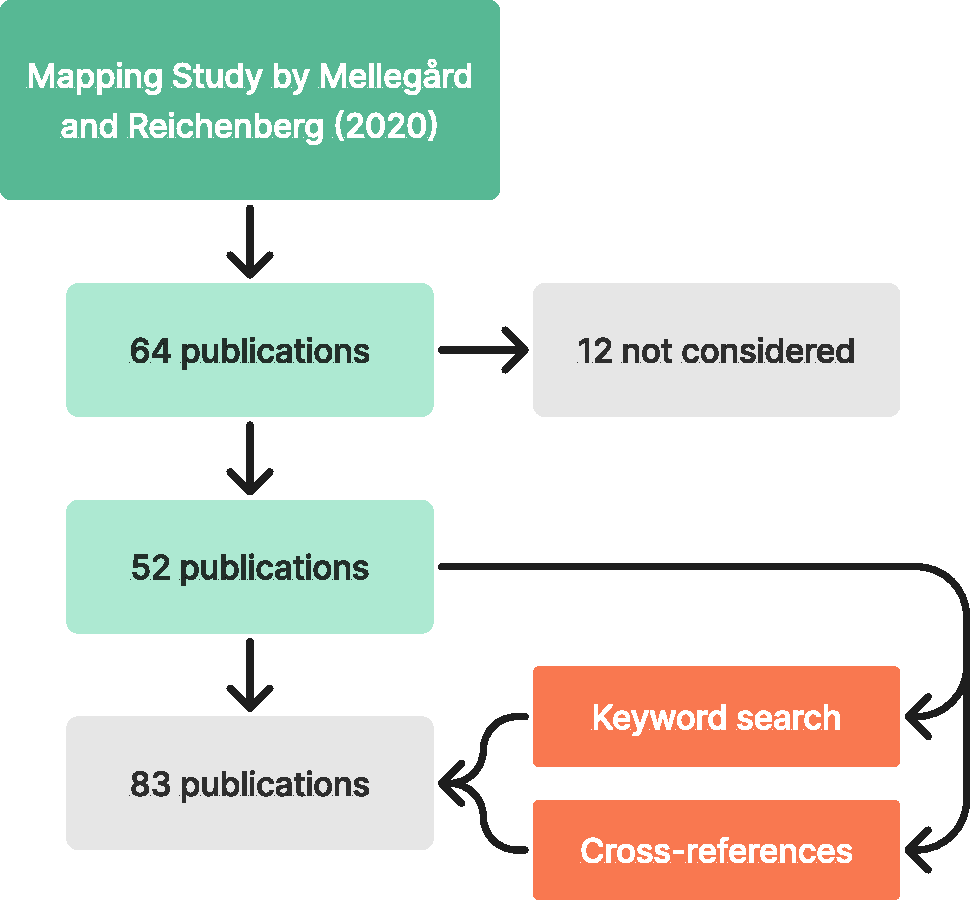
\includegraphics[width=\linewidth]{images/related-work-research-method.pdf} &
  \resizebox{\linewidth}{!}{%% Creator: Matplotlib, PGF backend
%%
%% To include the figure in your LaTeX document, write
%%   \input{<filename>.pgf}
%%
%% Make sure the required packages are loaded in your preamble
%%   \usepackage{pgf}
%%
%% Also ensure that all the required font packages are loaded; for instance,
%% the lmodern package is sometimes necessary when using math font.
%%   \usepackage{lmodern}
%%
%% Figures using additional raster images can only be included by \input if
%% they are in the same directory as the main LaTeX file. For loading figures
%% from other directories you can use the `import` package
%%   \usepackage{import}
%%
%% and then include the figures with
%%   \import{<path to file>}{<filename>.pgf}
%%
%% Matplotlib used the following preamble
%%   \def\mathdefault#1{#1}
%%   \everymath=\expandafter{\the\everymath\displaystyle}
%%   
%%   \makeatletter\@ifpackageloaded{underscore}{}{\usepackage[strings]{underscore}}\makeatother
%%
\begingroup%
\makeatletter%
\begin{pgfpicture}%
\pgfpathrectangle{\pgfpointorigin}{\pgfqpoint{4.490124in}{3.032040in}}%
\pgfusepath{use as bounding box, clip}%
\begin{pgfscope}%
\pgfsetbuttcap%
\pgfsetmiterjoin%
\definecolor{currentfill}{rgb}{1.000000,1.000000,1.000000}%
\pgfsetfillcolor{currentfill}%
\pgfsetlinewidth{0.000000pt}%
\definecolor{currentstroke}{rgb}{1.000000,1.000000,1.000000}%
\pgfsetstrokecolor{currentstroke}%
\pgfsetdash{}{0pt}%
\pgfpathmoveto{\pgfqpoint{0.000000in}{0.000000in}}%
\pgfpathlineto{\pgfqpoint{4.490124in}{0.000000in}}%
\pgfpathlineto{\pgfqpoint{4.490124in}{3.032040in}}%
\pgfpathlineto{\pgfqpoint{0.000000in}{3.032040in}}%
\pgfpathlineto{\pgfqpoint{0.000000in}{0.000000in}}%
\pgfpathclose%
\pgfusepath{fill}%
\end{pgfscope}%
\begin{pgfscope}%
\pgfsetbuttcap%
\pgfsetmiterjoin%
\definecolor{currentfill}{rgb}{1.000000,1.000000,1.000000}%
\pgfsetfillcolor{currentfill}%
\pgfsetlinewidth{0.000000pt}%
\definecolor{currentstroke}{rgb}{0.000000,0.000000,0.000000}%
\pgfsetstrokecolor{currentstroke}%
\pgfsetstrokeopacity{0.000000}%
\pgfsetdash{}{0pt}%
\pgfpathmoveto{\pgfqpoint{0.515124in}{0.622040in}}%
\pgfpathlineto{\pgfqpoint{4.390124in}{0.622040in}}%
\pgfpathlineto{\pgfqpoint{4.390124in}{2.932040in}}%
\pgfpathlineto{\pgfqpoint{0.515124in}{2.932040in}}%
\pgfpathlineto{\pgfqpoint{0.515124in}{0.622040in}}%
\pgfpathclose%
\pgfusepath{fill}%
\end{pgfscope}%
\begin{pgfscope}%
\pgfsetbuttcap%
\pgfsetroundjoin%
\definecolor{currentfill}{rgb}{0.000000,0.000000,0.000000}%
\pgfsetfillcolor{currentfill}%
\pgfsetlinewidth{0.803000pt}%
\definecolor{currentstroke}{rgb}{0.000000,0.000000,0.000000}%
\pgfsetstrokecolor{currentstroke}%
\pgfsetdash{}{0pt}%
\pgfsys@defobject{currentmarker}{\pgfqpoint{0.000000in}{-0.048611in}}{\pgfqpoint{0.000000in}{0.000000in}}{%
\pgfpathmoveto{\pgfqpoint{0.000000in}{0.000000in}}%
\pgfpathlineto{\pgfqpoint{0.000000in}{-0.048611in}}%
\pgfusepath{stroke,fill}%
}%
\begin{pgfscope}%
\pgfsys@transformshift{0.765684in}{0.622040in}%
\pgfsys@useobject{currentmarker}{}%
\end{pgfscope}%
\end{pgfscope}%
\begin{pgfscope}%
\definecolor{textcolor}{rgb}{0.000000,0.000000,0.000000}%
\pgfsetstrokecolor{textcolor}%
\pgfsetfillcolor{textcolor}%
\pgftext[x=0.662763in, y=0.302400in, left, base,rotate=30.000000]{\color{textcolor}{\sffamily\fontsize{10.000000}{12.000000}\selectfont\catcode`\^=\active\def^{\ifmmode\sp\else\^{}\fi}\catcode`\%=\active\def%{\%}$\mathdefault{2006}$}}%
\end{pgfscope}%
\begin{pgfscope}%
\pgfsetbuttcap%
\pgfsetroundjoin%
\definecolor{currentfill}{rgb}{0.000000,0.000000,0.000000}%
\pgfsetfillcolor{currentfill}%
\pgfsetlinewidth{0.803000pt}%
\definecolor{currentstroke}{rgb}{0.000000,0.000000,0.000000}%
\pgfsetstrokecolor{currentstroke}%
\pgfsetdash{}{0pt}%
\pgfsys@defobject{currentmarker}{\pgfqpoint{0.000000in}{-0.048611in}}{\pgfqpoint{0.000000in}{0.000000in}}{%
\pgfpathmoveto{\pgfqpoint{0.000000in}{0.000000in}}%
\pgfpathlineto{\pgfqpoint{0.000000in}{-0.048611in}}%
\pgfusepath{stroke,fill}%
}%
\begin{pgfscope}%
\pgfsys@transformshift{1.162611in}{0.622040in}%
\pgfsys@useobject{currentmarker}{}%
\end{pgfscope}%
\end{pgfscope}%
\begin{pgfscope}%
\definecolor{textcolor}{rgb}{0.000000,0.000000,0.000000}%
\pgfsetstrokecolor{textcolor}%
\pgfsetfillcolor{textcolor}%
\pgftext[x=1.059690in, y=0.302400in, left, base,rotate=30.000000]{\color{textcolor}{\sffamily\fontsize{10.000000}{12.000000}\selectfont\catcode`\^=\active\def^{\ifmmode\sp\else\^{}\fi}\catcode`\%=\active\def%{\%}$\mathdefault{2008}$}}%
\end{pgfscope}%
\begin{pgfscope}%
\pgfsetbuttcap%
\pgfsetroundjoin%
\definecolor{currentfill}{rgb}{0.000000,0.000000,0.000000}%
\pgfsetfillcolor{currentfill}%
\pgfsetlinewidth{0.803000pt}%
\definecolor{currentstroke}{rgb}{0.000000,0.000000,0.000000}%
\pgfsetstrokecolor{currentstroke}%
\pgfsetdash{}{0pt}%
\pgfsys@defobject{currentmarker}{\pgfqpoint{0.000000in}{-0.048611in}}{\pgfqpoint{0.000000in}{0.000000in}}{%
\pgfpathmoveto{\pgfqpoint{0.000000in}{0.000000in}}%
\pgfpathlineto{\pgfqpoint{0.000000in}{-0.048611in}}%
\pgfusepath{stroke,fill}%
}%
\begin{pgfscope}%
\pgfsys@transformshift{1.559538in}{0.622040in}%
\pgfsys@useobject{currentmarker}{}%
\end{pgfscope}%
\end{pgfscope}%
\begin{pgfscope}%
\definecolor{textcolor}{rgb}{0.000000,0.000000,0.000000}%
\pgfsetstrokecolor{textcolor}%
\pgfsetfillcolor{textcolor}%
\pgftext[x=1.456617in, y=0.302400in, left, base,rotate=30.000000]{\color{textcolor}{\sffamily\fontsize{10.000000}{12.000000}\selectfont\catcode`\^=\active\def^{\ifmmode\sp\else\^{}\fi}\catcode`\%=\active\def%{\%}$\mathdefault{2010}$}}%
\end{pgfscope}%
\begin{pgfscope}%
\pgfsetbuttcap%
\pgfsetroundjoin%
\definecolor{currentfill}{rgb}{0.000000,0.000000,0.000000}%
\pgfsetfillcolor{currentfill}%
\pgfsetlinewidth{0.803000pt}%
\definecolor{currentstroke}{rgb}{0.000000,0.000000,0.000000}%
\pgfsetstrokecolor{currentstroke}%
\pgfsetdash{}{0pt}%
\pgfsys@defobject{currentmarker}{\pgfqpoint{0.000000in}{-0.048611in}}{\pgfqpoint{0.000000in}{0.000000in}}{%
\pgfpathmoveto{\pgfqpoint{0.000000in}{0.000000in}}%
\pgfpathlineto{\pgfqpoint{0.000000in}{-0.048611in}}%
\pgfusepath{stroke,fill}%
}%
\begin{pgfscope}%
\pgfsys@transformshift{1.956465in}{0.622040in}%
\pgfsys@useobject{currentmarker}{}%
\end{pgfscope}%
\end{pgfscope}%
\begin{pgfscope}%
\definecolor{textcolor}{rgb}{0.000000,0.000000,0.000000}%
\pgfsetstrokecolor{textcolor}%
\pgfsetfillcolor{textcolor}%
\pgftext[x=1.853544in, y=0.302400in, left, base,rotate=30.000000]{\color{textcolor}{\sffamily\fontsize{10.000000}{12.000000}\selectfont\catcode`\^=\active\def^{\ifmmode\sp\else\^{}\fi}\catcode`\%=\active\def%{\%}$\mathdefault{2012}$}}%
\end{pgfscope}%
\begin{pgfscope}%
\pgfsetbuttcap%
\pgfsetroundjoin%
\definecolor{currentfill}{rgb}{0.000000,0.000000,0.000000}%
\pgfsetfillcolor{currentfill}%
\pgfsetlinewidth{0.803000pt}%
\definecolor{currentstroke}{rgb}{0.000000,0.000000,0.000000}%
\pgfsetstrokecolor{currentstroke}%
\pgfsetdash{}{0pt}%
\pgfsys@defobject{currentmarker}{\pgfqpoint{0.000000in}{-0.048611in}}{\pgfqpoint{0.000000in}{0.000000in}}{%
\pgfpathmoveto{\pgfqpoint{0.000000in}{0.000000in}}%
\pgfpathlineto{\pgfqpoint{0.000000in}{-0.048611in}}%
\pgfusepath{stroke,fill}%
}%
\begin{pgfscope}%
\pgfsys@transformshift{2.353392in}{0.622040in}%
\pgfsys@useobject{currentmarker}{}%
\end{pgfscope}%
\end{pgfscope}%
\begin{pgfscope}%
\definecolor{textcolor}{rgb}{0.000000,0.000000,0.000000}%
\pgfsetstrokecolor{textcolor}%
\pgfsetfillcolor{textcolor}%
\pgftext[x=2.250471in, y=0.302400in, left, base,rotate=30.000000]{\color{textcolor}{\sffamily\fontsize{10.000000}{12.000000}\selectfont\catcode`\^=\active\def^{\ifmmode\sp\else\^{}\fi}\catcode`\%=\active\def%{\%}$\mathdefault{2014}$}}%
\end{pgfscope}%
\begin{pgfscope}%
\pgfsetbuttcap%
\pgfsetroundjoin%
\definecolor{currentfill}{rgb}{0.000000,0.000000,0.000000}%
\pgfsetfillcolor{currentfill}%
\pgfsetlinewidth{0.803000pt}%
\definecolor{currentstroke}{rgb}{0.000000,0.000000,0.000000}%
\pgfsetstrokecolor{currentstroke}%
\pgfsetdash{}{0pt}%
\pgfsys@defobject{currentmarker}{\pgfqpoint{0.000000in}{-0.048611in}}{\pgfqpoint{0.000000in}{0.000000in}}{%
\pgfpathmoveto{\pgfqpoint{0.000000in}{0.000000in}}%
\pgfpathlineto{\pgfqpoint{0.000000in}{-0.048611in}}%
\pgfusepath{stroke,fill}%
}%
\begin{pgfscope}%
\pgfsys@transformshift{2.750319in}{0.622040in}%
\pgfsys@useobject{currentmarker}{}%
\end{pgfscope}%
\end{pgfscope}%
\begin{pgfscope}%
\definecolor{textcolor}{rgb}{0.000000,0.000000,0.000000}%
\pgfsetstrokecolor{textcolor}%
\pgfsetfillcolor{textcolor}%
\pgftext[x=2.647398in, y=0.302400in, left, base,rotate=30.000000]{\color{textcolor}{\sffamily\fontsize{10.000000}{12.000000}\selectfont\catcode`\^=\active\def^{\ifmmode\sp\else\^{}\fi}\catcode`\%=\active\def%{\%}$\mathdefault{2016}$}}%
\end{pgfscope}%
\begin{pgfscope}%
\pgfsetbuttcap%
\pgfsetroundjoin%
\definecolor{currentfill}{rgb}{0.000000,0.000000,0.000000}%
\pgfsetfillcolor{currentfill}%
\pgfsetlinewidth{0.803000pt}%
\definecolor{currentstroke}{rgb}{0.000000,0.000000,0.000000}%
\pgfsetstrokecolor{currentstroke}%
\pgfsetdash{}{0pt}%
\pgfsys@defobject{currentmarker}{\pgfqpoint{0.000000in}{-0.048611in}}{\pgfqpoint{0.000000in}{0.000000in}}{%
\pgfpathmoveto{\pgfqpoint{0.000000in}{0.000000in}}%
\pgfpathlineto{\pgfqpoint{0.000000in}{-0.048611in}}%
\pgfusepath{stroke,fill}%
}%
\begin{pgfscope}%
\pgfsys@transformshift{3.147246in}{0.622040in}%
\pgfsys@useobject{currentmarker}{}%
\end{pgfscope}%
\end{pgfscope}%
\begin{pgfscope}%
\definecolor{textcolor}{rgb}{0.000000,0.000000,0.000000}%
\pgfsetstrokecolor{textcolor}%
\pgfsetfillcolor{textcolor}%
\pgftext[x=3.044325in, y=0.302400in, left, base,rotate=30.000000]{\color{textcolor}{\sffamily\fontsize{10.000000}{12.000000}\selectfont\catcode`\^=\active\def^{\ifmmode\sp\else\^{}\fi}\catcode`\%=\active\def%{\%}$\mathdefault{2018}$}}%
\end{pgfscope}%
\begin{pgfscope}%
\pgfsetbuttcap%
\pgfsetroundjoin%
\definecolor{currentfill}{rgb}{0.000000,0.000000,0.000000}%
\pgfsetfillcolor{currentfill}%
\pgfsetlinewidth{0.803000pt}%
\definecolor{currentstroke}{rgb}{0.000000,0.000000,0.000000}%
\pgfsetstrokecolor{currentstroke}%
\pgfsetdash{}{0pt}%
\pgfsys@defobject{currentmarker}{\pgfqpoint{0.000000in}{-0.048611in}}{\pgfqpoint{0.000000in}{0.000000in}}{%
\pgfpathmoveto{\pgfqpoint{0.000000in}{0.000000in}}%
\pgfpathlineto{\pgfqpoint{0.000000in}{-0.048611in}}%
\pgfusepath{stroke,fill}%
}%
\begin{pgfscope}%
\pgfsys@transformshift{3.544173in}{0.622040in}%
\pgfsys@useobject{currentmarker}{}%
\end{pgfscope}%
\end{pgfscope}%
\begin{pgfscope}%
\definecolor{textcolor}{rgb}{0.000000,0.000000,0.000000}%
\pgfsetstrokecolor{textcolor}%
\pgfsetfillcolor{textcolor}%
\pgftext[x=3.441252in, y=0.302400in, left, base,rotate=30.000000]{\color{textcolor}{\sffamily\fontsize{10.000000}{12.000000}\selectfont\catcode`\^=\active\def^{\ifmmode\sp\else\^{}\fi}\catcode`\%=\active\def%{\%}$\mathdefault{2020}$}}%
\end{pgfscope}%
\begin{pgfscope}%
\pgfsetbuttcap%
\pgfsetroundjoin%
\definecolor{currentfill}{rgb}{0.000000,0.000000,0.000000}%
\pgfsetfillcolor{currentfill}%
\pgfsetlinewidth{0.803000pt}%
\definecolor{currentstroke}{rgb}{0.000000,0.000000,0.000000}%
\pgfsetstrokecolor{currentstroke}%
\pgfsetdash{}{0pt}%
\pgfsys@defobject{currentmarker}{\pgfqpoint{0.000000in}{-0.048611in}}{\pgfqpoint{0.000000in}{0.000000in}}{%
\pgfpathmoveto{\pgfqpoint{0.000000in}{0.000000in}}%
\pgfpathlineto{\pgfqpoint{0.000000in}{-0.048611in}}%
\pgfusepath{stroke,fill}%
}%
\begin{pgfscope}%
\pgfsys@transformshift{3.941100in}{0.622040in}%
\pgfsys@useobject{currentmarker}{}%
\end{pgfscope}%
\end{pgfscope}%
\begin{pgfscope}%
\definecolor{textcolor}{rgb}{0.000000,0.000000,0.000000}%
\pgfsetstrokecolor{textcolor}%
\pgfsetfillcolor{textcolor}%
\pgftext[x=3.838180in, y=0.302400in, left, base,rotate=30.000000]{\color{textcolor}{\sffamily\fontsize{10.000000}{12.000000}\selectfont\catcode`\^=\active\def^{\ifmmode\sp\else\^{}\fi}\catcode`\%=\active\def%{\%}$\mathdefault{2022}$}}%
\end{pgfscope}%
\begin{pgfscope}%
\definecolor{textcolor}{rgb}{0.000000,0.000000,0.000000}%
\pgfsetstrokecolor{textcolor}%
\pgfsetfillcolor{textcolor}%
\pgftext[x=2.452624in,y=0.223457in,,top]{\color{textcolor}{\sffamily\fontsize{10.000000}{12.000000}\selectfont\catcode`\^=\active\def^{\ifmmode\sp\else\^{}\fi}\catcode`\%=\active\def%{\%}Year}}%
\end{pgfscope}%
\begin{pgfscope}%
\pgfpathrectangle{\pgfqpoint{0.515124in}{0.622040in}}{\pgfqpoint{3.875000in}{2.310000in}}%
\pgfusepath{clip}%
\pgfsetbuttcap%
\pgfsetroundjoin%
\pgfsetlinewidth{0.501875pt}%
\definecolor{currentstroke}{rgb}{0.690196,0.690196,0.690196}%
\pgfsetstrokecolor{currentstroke}%
\pgfsetstrokeopacity{0.500000}%
\pgfsetdash{{1.850000pt}{0.800000pt}}{0.000000pt}%
\pgfpathmoveto{\pgfqpoint{0.515124in}{0.622040in}}%
\pgfpathlineto{\pgfqpoint{4.390124in}{0.622040in}}%
\pgfusepath{stroke}%
\end{pgfscope}%
\begin{pgfscope}%
\pgfsetbuttcap%
\pgfsetroundjoin%
\definecolor{currentfill}{rgb}{0.000000,0.000000,0.000000}%
\pgfsetfillcolor{currentfill}%
\pgfsetlinewidth{0.803000pt}%
\definecolor{currentstroke}{rgb}{0.000000,0.000000,0.000000}%
\pgfsetstrokecolor{currentstroke}%
\pgfsetdash{}{0pt}%
\pgfsys@defobject{currentmarker}{\pgfqpoint{-0.048611in}{0.000000in}}{\pgfqpoint{-0.000000in}{0.000000in}}{%
\pgfpathmoveto{\pgfqpoint{-0.000000in}{0.000000in}}%
\pgfpathlineto{\pgfqpoint{-0.048611in}{0.000000in}}%
\pgfusepath{stroke,fill}%
}%
\begin{pgfscope}%
\pgfsys@transformshift{0.515124in}{0.622040in}%
\pgfsys@useobject{currentmarker}{}%
\end{pgfscope}%
\end{pgfscope}%
\begin{pgfscope}%
\definecolor{textcolor}{rgb}{0.000000,0.000000,0.000000}%
\pgfsetstrokecolor{textcolor}%
\pgfsetfillcolor{textcolor}%
\pgftext[x=0.348457in, y=0.573815in, left, base]{\color{textcolor}{\sffamily\fontsize{10.000000}{12.000000}\selectfont\catcode`\^=\active\def^{\ifmmode\sp\else\^{}\fi}\catcode`\%=\active\def%{\%}$\mathdefault{0}$}}%
\end{pgfscope}%
\begin{pgfscope}%
\pgfpathrectangle{\pgfqpoint{0.515124in}{0.622040in}}{\pgfqpoint{3.875000in}{2.310000in}}%
\pgfusepath{clip}%
\pgfsetbuttcap%
\pgfsetroundjoin%
\pgfsetlinewidth{0.501875pt}%
\definecolor{currentstroke}{rgb}{0.690196,0.690196,0.690196}%
\pgfsetstrokecolor{currentstroke}%
\pgfsetstrokeopacity{0.500000}%
\pgfsetdash{{1.850000pt}{0.800000pt}}{0.000000pt}%
\pgfpathmoveto{\pgfqpoint{0.515124in}{1.042040in}}%
\pgfpathlineto{\pgfqpoint{4.390124in}{1.042040in}}%
\pgfusepath{stroke}%
\end{pgfscope}%
\begin{pgfscope}%
\pgfsetbuttcap%
\pgfsetroundjoin%
\definecolor{currentfill}{rgb}{0.000000,0.000000,0.000000}%
\pgfsetfillcolor{currentfill}%
\pgfsetlinewidth{0.803000pt}%
\definecolor{currentstroke}{rgb}{0.000000,0.000000,0.000000}%
\pgfsetstrokecolor{currentstroke}%
\pgfsetdash{}{0pt}%
\pgfsys@defobject{currentmarker}{\pgfqpoint{-0.048611in}{0.000000in}}{\pgfqpoint{-0.000000in}{0.000000in}}{%
\pgfpathmoveto{\pgfqpoint{-0.000000in}{0.000000in}}%
\pgfpathlineto{\pgfqpoint{-0.048611in}{0.000000in}}%
\pgfusepath{stroke,fill}%
}%
\begin{pgfscope}%
\pgfsys@transformshift{0.515124in}{1.042040in}%
\pgfsys@useobject{currentmarker}{}%
\end{pgfscope}%
\end{pgfscope}%
\begin{pgfscope}%
\definecolor{textcolor}{rgb}{0.000000,0.000000,0.000000}%
\pgfsetstrokecolor{textcolor}%
\pgfsetfillcolor{textcolor}%
\pgftext[x=0.348457in, y=0.993815in, left, base]{\color{textcolor}{\sffamily\fontsize{10.000000}{12.000000}\selectfont\catcode`\^=\active\def^{\ifmmode\sp\else\^{}\fi}\catcode`\%=\active\def%{\%}$\mathdefault{2}$}}%
\end{pgfscope}%
\begin{pgfscope}%
\pgfpathrectangle{\pgfqpoint{0.515124in}{0.622040in}}{\pgfqpoint{3.875000in}{2.310000in}}%
\pgfusepath{clip}%
\pgfsetbuttcap%
\pgfsetroundjoin%
\pgfsetlinewidth{0.501875pt}%
\definecolor{currentstroke}{rgb}{0.690196,0.690196,0.690196}%
\pgfsetstrokecolor{currentstroke}%
\pgfsetstrokeopacity{0.500000}%
\pgfsetdash{{1.850000pt}{0.800000pt}}{0.000000pt}%
\pgfpathmoveto{\pgfqpoint{0.515124in}{1.462040in}}%
\pgfpathlineto{\pgfqpoint{4.390124in}{1.462040in}}%
\pgfusepath{stroke}%
\end{pgfscope}%
\begin{pgfscope}%
\pgfsetbuttcap%
\pgfsetroundjoin%
\definecolor{currentfill}{rgb}{0.000000,0.000000,0.000000}%
\pgfsetfillcolor{currentfill}%
\pgfsetlinewidth{0.803000pt}%
\definecolor{currentstroke}{rgb}{0.000000,0.000000,0.000000}%
\pgfsetstrokecolor{currentstroke}%
\pgfsetdash{}{0pt}%
\pgfsys@defobject{currentmarker}{\pgfqpoint{-0.048611in}{0.000000in}}{\pgfqpoint{-0.000000in}{0.000000in}}{%
\pgfpathmoveto{\pgfqpoint{-0.000000in}{0.000000in}}%
\pgfpathlineto{\pgfqpoint{-0.048611in}{0.000000in}}%
\pgfusepath{stroke,fill}%
}%
\begin{pgfscope}%
\pgfsys@transformshift{0.515124in}{1.462040in}%
\pgfsys@useobject{currentmarker}{}%
\end{pgfscope}%
\end{pgfscope}%
\begin{pgfscope}%
\definecolor{textcolor}{rgb}{0.000000,0.000000,0.000000}%
\pgfsetstrokecolor{textcolor}%
\pgfsetfillcolor{textcolor}%
\pgftext[x=0.348457in, y=1.413815in, left, base]{\color{textcolor}{\sffamily\fontsize{10.000000}{12.000000}\selectfont\catcode`\^=\active\def^{\ifmmode\sp\else\^{}\fi}\catcode`\%=\active\def%{\%}$\mathdefault{4}$}}%
\end{pgfscope}%
\begin{pgfscope}%
\pgfpathrectangle{\pgfqpoint{0.515124in}{0.622040in}}{\pgfqpoint{3.875000in}{2.310000in}}%
\pgfusepath{clip}%
\pgfsetbuttcap%
\pgfsetroundjoin%
\pgfsetlinewidth{0.501875pt}%
\definecolor{currentstroke}{rgb}{0.690196,0.690196,0.690196}%
\pgfsetstrokecolor{currentstroke}%
\pgfsetstrokeopacity{0.500000}%
\pgfsetdash{{1.850000pt}{0.800000pt}}{0.000000pt}%
\pgfpathmoveto{\pgfqpoint{0.515124in}{1.882040in}}%
\pgfpathlineto{\pgfqpoint{4.390124in}{1.882040in}}%
\pgfusepath{stroke}%
\end{pgfscope}%
\begin{pgfscope}%
\pgfsetbuttcap%
\pgfsetroundjoin%
\definecolor{currentfill}{rgb}{0.000000,0.000000,0.000000}%
\pgfsetfillcolor{currentfill}%
\pgfsetlinewidth{0.803000pt}%
\definecolor{currentstroke}{rgb}{0.000000,0.000000,0.000000}%
\pgfsetstrokecolor{currentstroke}%
\pgfsetdash{}{0pt}%
\pgfsys@defobject{currentmarker}{\pgfqpoint{-0.048611in}{0.000000in}}{\pgfqpoint{-0.000000in}{0.000000in}}{%
\pgfpathmoveto{\pgfqpoint{-0.000000in}{0.000000in}}%
\pgfpathlineto{\pgfqpoint{-0.048611in}{0.000000in}}%
\pgfusepath{stroke,fill}%
}%
\begin{pgfscope}%
\pgfsys@transformshift{0.515124in}{1.882040in}%
\pgfsys@useobject{currentmarker}{}%
\end{pgfscope}%
\end{pgfscope}%
\begin{pgfscope}%
\definecolor{textcolor}{rgb}{0.000000,0.000000,0.000000}%
\pgfsetstrokecolor{textcolor}%
\pgfsetfillcolor{textcolor}%
\pgftext[x=0.348457in, y=1.833815in, left, base]{\color{textcolor}{\sffamily\fontsize{10.000000}{12.000000}\selectfont\catcode`\^=\active\def^{\ifmmode\sp\else\^{}\fi}\catcode`\%=\active\def%{\%}$\mathdefault{6}$}}%
\end{pgfscope}%
\begin{pgfscope}%
\pgfpathrectangle{\pgfqpoint{0.515124in}{0.622040in}}{\pgfqpoint{3.875000in}{2.310000in}}%
\pgfusepath{clip}%
\pgfsetbuttcap%
\pgfsetroundjoin%
\pgfsetlinewidth{0.501875pt}%
\definecolor{currentstroke}{rgb}{0.690196,0.690196,0.690196}%
\pgfsetstrokecolor{currentstroke}%
\pgfsetstrokeopacity{0.500000}%
\pgfsetdash{{1.850000pt}{0.800000pt}}{0.000000pt}%
\pgfpathmoveto{\pgfqpoint{0.515124in}{2.302040in}}%
\pgfpathlineto{\pgfqpoint{4.390124in}{2.302040in}}%
\pgfusepath{stroke}%
\end{pgfscope}%
\begin{pgfscope}%
\pgfsetbuttcap%
\pgfsetroundjoin%
\definecolor{currentfill}{rgb}{0.000000,0.000000,0.000000}%
\pgfsetfillcolor{currentfill}%
\pgfsetlinewidth{0.803000pt}%
\definecolor{currentstroke}{rgb}{0.000000,0.000000,0.000000}%
\pgfsetstrokecolor{currentstroke}%
\pgfsetdash{}{0pt}%
\pgfsys@defobject{currentmarker}{\pgfqpoint{-0.048611in}{0.000000in}}{\pgfqpoint{-0.000000in}{0.000000in}}{%
\pgfpathmoveto{\pgfqpoint{-0.000000in}{0.000000in}}%
\pgfpathlineto{\pgfqpoint{-0.048611in}{0.000000in}}%
\pgfusepath{stroke,fill}%
}%
\begin{pgfscope}%
\pgfsys@transformshift{0.515124in}{2.302040in}%
\pgfsys@useobject{currentmarker}{}%
\end{pgfscope}%
\end{pgfscope}%
\begin{pgfscope}%
\definecolor{textcolor}{rgb}{0.000000,0.000000,0.000000}%
\pgfsetstrokecolor{textcolor}%
\pgfsetfillcolor{textcolor}%
\pgftext[x=0.348457in, y=2.253815in, left, base]{\color{textcolor}{\sffamily\fontsize{10.000000}{12.000000}\selectfont\catcode`\^=\active\def^{\ifmmode\sp\else\^{}\fi}\catcode`\%=\active\def%{\%}$\mathdefault{8}$}}%
\end{pgfscope}%
\begin{pgfscope}%
\pgfpathrectangle{\pgfqpoint{0.515124in}{0.622040in}}{\pgfqpoint{3.875000in}{2.310000in}}%
\pgfusepath{clip}%
\pgfsetbuttcap%
\pgfsetroundjoin%
\pgfsetlinewidth{0.501875pt}%
\definecolor{currentstroke}{rgb}{0.690196,0.690196,0.690196}%
\pgfsetstrokecolor{currentstroke}%
\pgfsetstrokeopacity{0.500000}%
\pgfsetdash{{1.850000pt}{0.800000pt}}{0.000000pt}%
\pgfpathmoveto{\pgfqpoint{0.515124in}{2.722040in}}%
\pgfpathlineto{\pgfqpoint{4.390124in}{2.722040in}}%
\pgfusepath{stroke}%
\end{pgfscope}%
\begin{pgfscope}%
\pgfsetbuttcap%
\pgfsetroundjoin%
\definecolor{currentfill}{rgb}{0.000000,0.000000,0.000000}%
\pgfsetfillcolor{currentfill}%
\pgfsetlinewidth{0.803000pt}%
\definecolor{currentstroke}{rgb}{0.000000,0.000000,0.000000}%
\pgfsetstrokecolor{currentstroke}%
\pgfsetdash{}{0pt}%
\pgfsys@defobject{currentmarker}{\pgfqpoint{-0.048611in}{0.000000in}}{\pgfqpoint{-0.000000in}{0.000000in}}{%
\pgfpathmoveto{\pgfqpoint{-0.000000in}{0.000000in}}%
\pgfpathlineto{\pgfqpoint{-0.048611in}{0.000000in}}%
\pgfusepath{stroke,fill}%
}%
\begin{pgfscope}%
\pgfsys@transformshift{0.515124in}{2.722040in}%
\pgfsys@useobject{currentmarker}{}%
\end{pgfscope}%
\end{pgfscope}%
\begin{pgfscope}%
\definecolor{textcolor}{rgb}{0.000000,0.000000,0.000000}%
\pgfsetstrokecolor{textcolor}%
\pgfsetfillcolor{textcolor}%
\pgftext[x=0.279012in, y=2.673815in, left, base]{\color{textcolor}{\sffamily\fontsize{10.000000}{12.000000}\selectfont\catcode`\^=\active\def^{\ifmmode\sp\else\^{}\fi}\catcode`\%=\active\def%{\%}$\mathdefault{10}$}}%
\end{pgfscope}%
\begin{pgfscope}%
\definecolor{textcolor}{rgb}{0.000000,0.000000,0.000000}%
\pgfsetstrokecolor{textcolor}%
\pgfsetfillcolor{textcolor}%
\pgftext[x=0.223457in,y=1.777040in,,bottom,rotate=90.000000]{\color{textcolor}{\sffamily\fontsize{10.000000}{12.000000}\selectfont\catcode`\^=\active\def^{\ifmmode\sp\else\^{}\fi}\catcode`\%=\active\def%{\%}\# Publications}}%
\end{pgfscope}%
\begin{pgfscope}%
\pgfpathrectangle{\pgfqpoint{0.515124in}{0.622040in}}{\pgfqpoint{3.875000in}{2.310000in}}%
\pgfusepath{clip}%
\pgfsetbuttcap%
\pgfsetmiterjoin%
\definecolor{currentfill}{rgb}{0.000000,0.411765,0.705882}%
\pgfsetfillcolor{currentfill}%
\pgfsetlinewidth{0.000000pt}%
\definecolor{currentstroke}{rgb}{0.000000,0.000000,0.000000}%
\pgfsetstrokecolor{currentstroke}%
\pgfsetstrokeopacity{0.000000}%
\pgfsetdash{}{0pt}%
\pgfpathmoveto{\pgfqpoint{0.691260in}{0.622040in}}%
\pgfpathlineto{\pgfqpoint{0.840108in}{0.622040in}}%
\pgfpathlineto{\pgfqpoint{0.840108in}{0.832040in}}%
\pgfpathlineto{\pgfqpoint{0.691260in}{0.832040in}}%
\pgfpathlineto{\pgfqpoint{0.691260in}{0.622040in}}%
\pgfpathclose%
\pgfusepath{fill}%
\end{pgfscope}%
\begin{pgfscope}%
\pgfpathrectangle{\pgfqpoint{0.515124in}{0.622040in}}{\pgfqpoint{3.875000in}{2.310000in}}%
\pgfusepath{clip}%
\pgfsetbuttcap%
\pgfsetmiterjoin%
\definecolor{currentfill}{rgb}{0.000000,0.411765,0.705882}%
\pgfsetfillcolor{currentfill}%
\pgfsetlinewidth{0.000000pt}%
\definecolor{currentstroke}{rgb}{0.000000,0.000000,0.000000}%
\pgfsetstrokecolor{currentstroke}%
\pgfsetstrokeopacity{0.000000}%
\pgfsetdash{}{0pt}%
\pgfpathmoveto{\pgfqpoint{0.889724in}{0.622040in}}%
\pgfpathlineto{\pgfqpoint{1.038571in}{0.622040in}}%
\pgfpathlineto{\pgfqpoint{1.038571in}{0.622040in}}%
\pgfpathlineto{\pgfqpoint{0.889724in}{0.622040in}}%
\pgfpathlineto{\pgfqpoint{0.889724in}{0.622040in}}%
\pgfpathclose%
\pgfusepath{fill}%
\end{pgfscope}%
\begin{pgfscope}%
\pgfpathrectangle{\pgfqpoint{0.515124in}{0.622040in}}{\pgfqpoint{3.875000in}{2.310000in}}%
\pgfusepath{clip}%
\pgfsetbuttcap%
\pgfsetmiterjoin%
\definecolor{currentfill}{rgb}{0.000000,0.411765,0.705882}%
\pgfsetfillcolor{currentfill}%
\pgfsetlinewidth{0.000000pt}%
\definecolor{currentstroke}{rgb}{0.000000,0.000000,0.000000}%
\pgfsetstrokecolor{currentstroke}%
\pgfsetstrokeopacity{0.000000}%
\pgfsetdash{}{0pt}%
\pgfpathmoveto{\pgfqpoint{1.088187in}{0.622040in}}%
\pgfpathlineto{\pgfqpoint{1.237035in}{0.622040in}}%
\pgfpathlineto{\pgfqpoint{1.237035in}{0.832040in}}%
\pgfpathlineto{\pgfqpoint{1.088187in}{0.832040in}}%
\pgfpathlineto{\pgfqpoint{1.088187in}{0.622040in}}%
\pgfpathclose%
\pgfusepath{fill}%
\end{pgfscope}%
\begin{pgfscope}%
\pgfpathrectangle{\pgfqpoint{0.515124in}{0.622040in}}{\pgfqpoint{3.875000in}{2.310000in}}%
\pgfusepath{clip}%
\pgfsetbuttcap%
\pgfsetmiterjoin%
\definecolor{currentfill}{rgb}{0.000000,0.411765,0.705882}%
\pgfsetfillcolor{currentfill}%
\pgfsetlinewidth{0.000000pt}%
\definecolor{currentstroke}{rgb}{0.000000,0.000000,0.000000}%
\pgfsetstrokecolor{currentstroke}%
\pgfsetstrokeopacity{0.000000}%
\pgfsetdash{}{0pt}%
\pgfpathmoveto{\pgfqpoint{1.286651in}{0.622040in}}%
\pgfpathlineto{\pgfqpoint{1.435498in}{0.622040in}}%
\pgfpathlineto{\pgfqpoint{1.435498in}{0.622040in}}%
\pgfpathlineto{\pgfqpoint{1.286651in}{0.622040in}}%
\pgfpathlineto{\pgfqpoint{1.286651in}{0.622040in}}%
\pgfpathclose%
\pgfusepath{fill}%
\end{pgfscope}%
\begin{pgfscope}%
\pgfpathrectangle{\pgfqpoint{0.515124in}{0.622040in}}{\pgfqpoint{3.875000in}{2.310000in}}%
\pgfusepath{clip}%
\pgfsetbuttcap%
\pgfsetmiterjoin%
\definecolor{currentfill}{rgb}{0.000000,0.411765,0.705882}%
\pgfsetfillcolor{currentfill}%
\pgfsetlinewidth{0.000000pt}%
\definecolor{currentstroke}{rgb}{0.000000,0.000000,0.000000}%
\pgfsetstrokecolor{currentstroke}%
\pgfsetstrokeopacity{0.000000}%
\pgfsetdash{}{0pt}%
\pgfpathmoveto{\pgfqpoint{1.485114in}{0.622040in}}%
\pgfpathlineto{\pgfqpoint{1.633962in}{0.622040in}}%
\pgfpathlineto{\pgfqpoint{1.633962in}{0.832040in}}%
\pgfpathlineto{\pgfqpoint{1.485114in}{0.832040in}}%
\pgfpathlineto{\pgfqpoint{1.485114in}{0.622040in}}%
\pgfpathclose%
\pgfusepath{fill}%
\end{pgfscope}%
\begin{pgfscope}%
\pgfpathrectangle{\pgfqpoint{0.515124in}{0.622040in}}{\pgfqpoint{3.875000in}{2.310000in}}%
\pgfusepath{clip}%
\pgfsetbuttcap%
\pgfsetmiterjoin%
\definecolor{currentfill}{rgb}{0.000000,0.411765,0.705882}%
\pgfsetfillcolor{currentfill}%
\pgfsetlinewidth{0.000000pt}%
\definecolor{currentstroke}{rgb}{0.000000,0.000000,0.000000}%
\pgfsetstrokecolor{currentstroke}%
\pgfsetstrokeopacity{0.000000}%
\pgfsetdash{}{0pt}%
\pgfpathmoveto{\pgfqpoint{1.683578in}{0.622040in}}%
\pgfpathlineto{\pgfqpoint{1.832425in}{0.622040in}}%
\pgfpathlineto{\pgfqpoint{1.832425in}{2.092040in}}%
\pgfpathlineto{\pgfqpoint{1.683578in}{2.092040in}}%
\pgfpathlineto{\pgfqpoint{1.683578in}{0.622040in}}%
\pgfpathclose%
\pgfusepath{fill}%
\end{pgfscope}%
\begin{pgfscope}%
\pgfpathrectangle{\pgfqpoint{0.515124in}{0.622040in}}{\pgfqpoint{3.875000in}{2.310000in}}%
\pgfusepath{clip}%
\pgfsetbuttcap%
\pgfsetmiterjoin%
\definecolor{currentfill}{rgb}{0.000000,0.411765,0.705882}%
\pgfsetfillcolor{currentfill}%
\pgfsetlinewidth{0.000000pt}%
\definecolor{currentstroke}{rgb}{0.000000,0.000000,0.000000}%
\pgfsetstrokecolor{currentstroke}%
\pgfsetstrokeopacity{0.000000}%
\pgfsetdash{}{0pt}%
\pgfpathmoveto{\pgfqpoint{1.882041in}{0.622040in}}%
\pgfpathlineto{\pgfqpoint{2.030889in}{0.622040in}}%
\pgfpathlineto{\pgfqpoint{2.030889in}{1.882040in}}%
\pgfpathlineto{\pgfqpoint{1.882041in}{1.882040in}}%
\pgfpathlineto{\pgfqpoint{1.882041in}{0.622040in}}%
\pgfpathclose%
\pgfusepath{fill}%
\end{pgfscope}%
\begin{pgfscope}%
\pgfpathrectangle{\pgfqpoint{0.515124in}{0.622040in}}{\pgfqpoint{3.875000in}{2.310000in}}%
\pgfusepath{clip}%
\pgfsetbuttcap%
\pgfsetmiterjoin%
\definecolor{currentfill}{rgb}{0.000000,0.411765,0.705882}%
\pgfsetfillcolor{currentfill}%
\pgfsetlinewidth{0.000000pt}%
\definecolor{currentstroke}{rgb}{0.000000,0.000000,0.000000}%
\pgfsetstrokecolor{currentstroke}%
\pgfsetstrokeopacity{0.000000}%
\pgfsetdash{}{0pt}%
\pgfpathmoveto{\pgfqpoint{2.080505in}{0.622040in}}%
\pgfpathlineto{\pgfqpoint{2.229352in}{0.622040in}}%
\pgfpathlineto{\pgfqpoint{2.229352in}{2.092040in}}%
\pgfpathlineto{\pgfqpoint{2.080505in}{2.092040in}}%
\pgfpathlineto{\pgfqpoint{2.080505in}{0.622040in}}%
\pgfpathclose%
\pgfusepath{fill}%
\end{pgfscope}%
\begin{pgfscope}%
\pgfpathrectangle{\pgfqpoint{0.515124in}{0.622040in}}{\pgfqpoint{3.875000in}{2.310000in}}%
\pgfusepath{clip}%
\pgfsetbuttcap%
\pgfsetmiterjoin%
\definecolor{currentfill}{rgb}{0.000000,0.411765,0.705882}%
\pgfsetfillcolor{currentfill}%
\pgfsetlinewidth{0.000000pt}%
\definecolor{currentstroke}{rgb}{0.000000,0.000000,0.000000}%
\pgfsetstrokecolor{currentstroke}%
\pgfsetstrokeopacity{0.000000}%
\pgfsetdash{}{0pt}%
\pgfpathmoveto{\pgfqpoint{2.278968in}{0.622040in}}%
\pgfpathlineto{\pgfqpoint{2.427816in}{0.622040in}}%
\pgfpathlineto{\pgfqpoint{2.427816in}{2.092040in}}%
\pgfpathlineto{\pgfqpoint{2.278968in}{2.092040in}}%
\pgfpathlineto{\pgfqpoint{2.278968in}{0.622040in}}%
\pgfpathclose%
\pgfusepath{fill}%
\end{pgfscope}%
\begin{pgfscope}%
\pgfpathrectangle{\pgfqpoint{0.515124in}{0.622040in}}{\pgfqpoint{3.875000in}{2.310000in}}%
\pgfusepath{clip}%
\pgfsetbuttcap%
\pgfsetmiterjoin%
\definecolor{currentfill}{rgb}{0.000000,0.411765,0.705882}%
\pgfsetfillcolor{currentfill}%
\pgfsetlinewidth{0.000000pt}%
\definecolor{currentstroke}{rgb}{0.000000,0.000000,0.000000}%
\pgfsetstrokecolor{currentstroke}%
\pgfsetstrokeopacity{0.000000}%
\pgfsetdash{}{0pt}%
\pgfpathmoveto{\pgfqpoint{2.477432in}{0.622040in}}%
\pgfpathlineto{\pgfqpoint{2.626279in}{0.622040in}}%
\pgfpathlineto{\pgfqpoint{2.626279in}{1.252040in}}%
\pgfpathlineto{\pgfqpoint{2.477432in}{1.252040in}}%
\pgfpathlineto{\pgfqpoint{2.477432in}{0.622040in}}%
\pgfpathclose%
\pgfusepath{fill}%
\end{pgfscope}%
\begin{pgfscope}%
\pgfpathrectangle{\pgfqpoint{0.515124in}{0.622040in}}{\pgfqpoint{3.875000in}{2.310000in}}%
\pgfusepath{clip}%
\pgfsetbuttcap%
\pgfsetmiterjoin%
\definecolor{currentfill}{rgb}{0.000000,0.411765,0.705882}%
\pgfsetfillcolor{currentfill}%
\pgfsetlinewidth{0.000000pt}%
\definecolor{currentstroke}{rgb}{0.000000,0.000000,0.000000}%
\pgfsetstrokecolor{currentstroke}%
\pgfsetstrokeopacity{0.000000}%
\pgfsetdash{}{0pt}%
\pgfpathmoveto{\pgfqpoint{2.675895in}{0.622040in}}%
\pgfpathlineto{\pgfqpoint{2.824743in}{0.622040in}}%
\pgfpathlineto{\pgfqpoint{2.824743in}{1.882040in}}%
\pgfpathlineto{\pgfqpoint{2.675895in}{1.882040in}}%
\pgfpathlineto{\pgfqpoint{2.675895in}{0.622040in}}%
\pgfpathclose%
\pgfusepath{fill}%
\end{pgfscope}%
\begin{pgfscope}%
\pgfpathrectangle{\pgfqpoint{0.515124in}{0.622040in}}{\pgfqpoint{3.875000in}{2.310000in}}%
\pgfusepath{clip}%
\pgfsetbuttcap%
\pgfsetmiterjoin%
\definecolor{currentfill}{rgb}{0.000000,0.411765,0.705882}%
\pgfsetfillcolor{currentfill}%
\pgfsetlinewidth{0.000000pt}%
\definecolor{currentstroke}{rgb}{0.000000,0.000000,0.000000}%
\pgfsetstrokecolor{currentstroke}%
\pgfsetstrokeopacity{0.000000}%
\pgfsetdash{}{0pt}%
\pgfpathmoveto{\pgfqpoint{2.874359in}{0.622040in}}%
\pgfpathlineto{\pgfqpoint{3.023206in}{0.622040in}}%
\pgfpathlineto{\pgfqpoint{3.023206in}{1.042040in}}%
\pgfpathlineto{\pgfqpoint{2.874359in}{1.042040in}}%
\pgfpathlineto{\pgfqpoint{2.874359in}{0.622040in}}%
\pgfpathclose%
\pgfusepath{fill}%
\end{pgfscope}%
\begin{pgfscope}%
\pgfpathrectangle{\pgfqpoint{0.515124in}{0.622040in}}{\pgfqpoint{3.875000in}{2.310000in}}%
\pgfusepath{clip}%
\pgfsetbuttcap%
\pgfsetmiterjoin%
\definecolor{currentfill}{rgb}{0.000000,0.411765,0.705882}%
\pgfsetfillcolor{currentfill}%
\pgfsetlinewidth{0.000000pt}%
\definecolor{currentstroke}{rgb}{0.000000,0.000000,0.000000}%
\pgfsetstrokecolor{currentstroke}%
\pgfsetstrokeopacity{0.000000}%
\pgfsetdash{}{0pt}%
\pgfpathmoveto{\pgfqpoint{3.072822in}{0.622040in}}%
\pgfpathlineto{\pgfqpoint{3.221670in}{0.622040in}}%
\pgfpathlineto{\pgfqpoint{3.221670in}{2.302040in}}%
\pgfpathlineto{\pgfqpoint{3.072822in}{2.302040in}}%
\pgfpathlineto{\pgfqpoint{3.072822in}{0.622040in}}%
\pgfpathclose%
\pgfusepath{fill}%
\end{pgfscope}%
\begin{pgfscope}%
\pgfpathrectangle{\pgfqpoint{0.515124in}{0.622040in}}{\pgfqpoint{3.875000in}{2.310000in}}%
\pgfusepath{clip}%
\pgfsetbuttcap%
\pgfsetmiterjoin%
\definecolor{currentfill}{rgb}{0.000000,0.411765,0.705882}%
\pgfsetfillcolor{currentfill}%
\pgfsetlinewidth{0.000000pt}%
\definecolor{currentstroke}{rgb}{0.000000,0.000000,0.000000}%
\pgfsetstrokecolor{currentstroke}%
\pgfsetstrokeopacity{0.000000}%
\pgfsetdash{}{0pt}%
\pgfpathmoveto{\pgfqpoint{3.271286in}{0.622040in}}%
\pgfpathlineto{\pgfqpoint{3.420133in}{0.622040in}}%
\pgfpathlineto{\pgfqpoint{3.420133in}{1.042040in}}%
\pgfpathlineto{\pgfqpoint{3.271286in}{1.042040in}}%
\pgfpathlineto{\pgfqpoint{3.271286in}{0.622040in}}%
\pgfpathclose%
\pgfusepath{fill}%
\end{pgfscope}%
\begin{pgfscope}%
\pgfpathrectangle{\pgfqpoint{0.515124in}{0.622040in}}{\pgfqpoint{3.875000in}{2.310000in}}%
\pgfusepath{clip}%
\pgfsetbuttcap%
\pgfsetmiterjoin%
\definecolor{currentfill}{rgb}{0.000000,0.411765,0.705882}%
\pgfsetfillcolor{currentfill}%
\pgfsetlinewidth{0.000000pt}%
\definecolor{currentstroke}{rgb}{0.000000,0.000000,0.000000}%
\pgfsetstrokecolor{currentstroke}%
\pgfsetstrokeopacity{0.000000}%
\pgfsetdash{}{0pt}%
\pgfpathmoveto{\pgfqpoint{3.469749in}{0.622040in}}%
\pgfpathlineto{\pgfqpoint{3.618597in}{0.622040in}}%
\pgfpathlineto{\pgfqpoint{3.618597in}{0.622040in}}%
\pgfpathlineto{\pgfqpoint{3.469749in}{0.622040in}}%
\pgfpathlineto{\pgfqpoint{3.469749in}{0.622040in}}%
\pgfpathclose%
\pgfusepath{fill}%
\end{pgfscope}%
\begin{pgfscope}%
\pgfpathrectangle{\pgfqpoint{0.515124in}{0.622040in}}{\pgfqpoint{3.875000in}{2.310000in}}%
\pgfusepath{clip}%
\pgfsetbuttcap%
\pgfsetmiterjoin%
\definecolor{currentfill}{rgb}{0.000000,0.411765,0.705882}%
\pgfsetfillcolor{currentfill}%
\pgfsetlinewidth{0.000000pt}%
\definecolor{currentstroke}{rgb}{0.000000,0.000000,0.000000}%
\pgfsetstrokecolor{currentstroke}%
\pgfsetstrokeopacity{0.000000}%
\pgfsetdash{}{0pt}%
\pgfpathmoveto{\pgfqpoint{3.668213in}{0.622040in}}%
\pgfpathlineto{\pgfqpoint{3.817060in}{0.622040in}}%
\pgfpathlineto{\pgfqpoint{3.817060in}{0.622040in}}%
\pgfpathlineto{\pgfqpoint{3.668213in}{0.622040in}}%
\pgfpathlineto{\pgfqpoint{3.668213in}{0.622040in}}%
\pgfpathclose%
\pgfusepath{fill}%
\end{pgfscope}%
\begin{pgfscope}%
\pgfpathrectangle{\pgfqpoint{0.515124in}{0.622040in}}{\pgfqpoint{3.875000in}{2.310000in}}%
\pgfusepath{clip}%
\pgfsetbuttcap%
\pgfsetmiterjoin%
\definecolor{currentfill}{rgb}{0.000000,0.411765,0.705882}%
\pgfsetfillcolor{currentfill}%
\pgfsetlinewidth{0.000000pt}%
\definecolor{currentstroke}{rgb}{0.000000,0.000000,0.000000}%
\pgfsetstrokecolor{currentstroke}%
\pgfsetstrokeopacity{0.000000}%
\pgfsetdash{}{0pt}%
\pgfpathmoveto{\pgfqpoint{3.866676in}{0.622040in}}%
\pgfpathlineto{\pgfqpoint{4.015524in}{0.622040in}}%
\pgfpathlineto{\pgfqpoint{4.015524in}{0.622040in}}%
\pgfpathlineto{\pgfqpoint{3.866676in}{0.622040in}}%
\pgfpathlineto{\pgfqpoint{3.866676in}{0.622040in}}%
\pgfpathclose%
\pgfusepath{fill}%
\end{pgfscope}%
\begin{pgfscope}%
\pgfpathrectangle{\pgfqpoint{0.515124in}{0.622040in}}{\pgfqpoint{3.875000in}{2.310000in}}%
\pgfusepath{clip}%
\pgfsetbuttcap%
\pgfsetmiterjoin%
\definecolor{currentfill}{rgb}{0.000000,0.411765,0.705882}%
\pgfsetfillcolor{currentfill}%
\pgfsetlinewidth{0.000000pt}%
\definecolor{currentstroke}{rgb}{0.000000,0.000000,0.000000}%
\pgfsetstrokecolor{currentstroke}%
\pgfsetstrokeopacity{0.000000}%
\pgfsetdash{}{0pt}%
\pgfpathmoveto{\pgfqpoint{4.065140in}{0.622040in}}%
\pgfpathlineto{\pgfqpoint{4.213987in}{0.622040in}}%
\pgfpathlineto{\pgfqpoint{4.213987in}{0.622040in}}%
\pgfpathlineto{\pgfqpoint{4.065140in}{0.622040in}}%
\pgfpathlineto{\pgfqpoint{4.065140in}{0.622040in}}%
\pgfpathclose%
\pgfusepath{fill}%
\end{pgfscope}%
\begin{pgfscope}%
\pgfpathrectangle{\pgfqpoint{0.515124in}{0.622040in}}{\pgfqpoint{3.875000in}{2.310000in}}%
\pgfusepath{clip}%
\pgfsetbuttcap%
\pgfsetmiterjoin%
\definecolor{currentfill}{rgb}{0.000000,0.188235,0.364706}%
\pgfsetfillcolor{currentfill}%
\pgfsetlinewidth{0.000000pt}%
\definecolor{currentstroke}{rgb}{0.000000,0.000000,0.000000}%
\pgfsetstrokecolor{currentstroke}%
\pgfsetstrokeopacity{0.000000}%
\pgfsetdash{}{0pt}%
\pgfpathmoveto{\pgfqpoint{0.691260in}{0.832040in}}%
\pgfpathlineto{\pgfqpoint{0.840108in}{0.832040in}}%
\pgfpathlineto{\pgfqpoint{0.840108in}{0.832040in}}%
\pgfpathlineto{\pgfqpoint{0.691260in}{0.832040in}}%
\pgfpathlineto{\pgfqpoint{0.691260in}{0.832040in}}%
\pgfpathclose%
\pgfusepath{fill}%
\end{pgfscope}%
\begin{pgfscope}%
\pgfpathrectangle{\pgfqpoint{0.515124in}{0.622040in}}{\pgfqpoint{3.875000in}{2.310000in}}%
\pgfusepath{clip}%
\pgfsetbuttcap%
\pgfsetmiterjoin%
\definecolor{currentfill}{rgb}{0.000000,0.188235,0.364706}%
\pgfsetfillcolor{currentfill}%
\pgfsetlinewidth{0.000000pt}%
\definecolor{currentstroke}{rgb}{0.000000,0.000000,0.000000}%
\pgfsetstrokecolor{currentstroke}%
\pgfsetstrokeopacity{0.000000}%
\pgfsetdash{}{0pt}%
\pgfpathmoveto{\pgfqpoint{0.889724in}{0.622040in}}%
\pgfpathlineto{\pgfqpoint{1.038571in}{0.622040in}}%
\pgfpathlineto{\pgfqpoint{1.038571in}{0.622040in}}%
\pgfpathlineto{\pgfqpoint{0.889724in}{0.622040in}}%
\pgfpathlineto{\pgfqpoint{0.889724in}{0.622040in}}%
\pgfpathclose%
\pgfusepath{fill}%
\end{pgfscope}%
\begin{pgfscope}%
\pgfpathrectangle{\pgfqpoint{0.515124in}{0.622040in}}{\pgfqpoint{3.875000in}{2.310000in}}%
\pgfusepath{clip}%
\pgfsetbuttcap%
\pgfsetmiterjoin%
\definecolor{currentfill}{rgb}{0.000000,0.188235,0.364706}%
\pgfsetfillcolor{currentfill}%
\pgfsetlinewidth{0.000000pt}%
\definecolor{currentstroke}{rgb}{0.000000,0.000000,0.000000}%
\pgfsetstrokecolor{currentstroke}%
\pgfsetstrokeopacity{0.000000}%
\pgfsetdash{}{0pt}%
\pgfpathmoveto{\pgfqpoint{1.088187in}{0.832040in}}%
\pgfpathlineto{\pgfqpoint{1.237035in}{0.832040in}}%
\pgfpathlineto{\pgfqpoint{1.237035in}{0.832040in}}%
\pgfpathlineto{\pgfqpoint{1.088187in}{0.832040in}}%
\pgfpathlineto{\pgfqpoint{1.088187in}{0.832040in}}%
\pgfpathclose%
\pgfusepath{fill}%
\end{pgfscope}%
\begin{pgfscope}%
\pgfpathrectangle{\pgfqpoint{0.515124in}{0.622040in}}{\pgfqpoint{3.875000in}{2.310000in}}%
\pgfusepath{clip}%
\pgfsetbuttcap%
\pgfsetmiterjoin%
\definecolor{currentfill}{rgb}{0.000000,0.188235,0.364706}%
\pgfsetfillcolor{currentfill}%
\pgfsetlinewidth{0.000000pt}%
\definecolor{currentstroke}{rgb}{0.000000,0.000000,0.000000}%
\pgfsetstrokecolor{currentstroke}%
\pgfsetstrokeopacity{0.000000}%
\pgfsetdash{}{0pt}%
\pgfpathmoveto{\pgfqpoint{1.286651in}{0.622040in}}%
\pgfpathlineto{\pgfqpoint{1.435498in}{0.622040in}}%
\pgfpathlineto{\pgfqpoint{1.435498in}{0.622040in}}%
\pgfpathlineto{\pgfqpoint{1.286651in}{0.622040in}}%
\pgfpathlineto{\pgfqpoint{1.286651in}{0.622040in}}%
\pgfpathclose%
\pgfusepath{fill}%
\end{pgfscope}%
\begin{pgfscope}%
\pgfpathrectangle{\pgfqpoint{0.515124in}{0.622040in}}{\pgfqpoint{3.875000in}{2.310000in}}%
\pgfusepath{clip}%
\pgfsetbuttcap%
\pgfsetmiterjoin%
\definecolor{currentfill}{rgb}{0.000000,0.188235,0.364706}%
\pgfsetfillcolor{currentfill}%
\pgfsetlinewidth{0.000000pt}%
\definecolor{currentstroke}{rgb}{0.000000,0.000000,0.000000}%
\pgfsetstrokecolor{currentstroke}%
\pgfsetstrokeopacity{0.000000}%
\pgfsetdash{}{0pt}%
\pgfpathmoveto{\pgfqpoint{1.485114in}{0.832040in}}%
\pgfpathlineto{\pgfqpoint{1.633962in}{0.832040in}}%
\pgfpathlineto{\pgfqpoint{1.633962in}{1.042040in}}%
\pgfpathlineto{\pgfqpoint{1.485114in}{1.042040in}}%
\pgfpathlineto{\pgfqpoint{1.485114in}{0.832040in}}%
\pgfpathclose%
\pgfusepath{fill}%
\end{pgfscope}%
\begin{pgfscope}%
\pgfpathrectangle{\pgfqpoint{0.515124in}{0.622040in}}{\pgfqpoint{3.875000in}{2.310000in}}%
\pgfusepath{clip}%
\pgfsetbuttcap%
\pgfsetmiterjoin%
\definecolor{currentfill}{rgb}{0.000000,0.188235,0.364706}%
\pgfsetfillcolor{currentfill}%
\pgfsetlinewidth{0.000000pt}%
\definecolor{currentstroke}{rgb}{0.000000,0.000000,0.000000}%
\pgfsetstrokecolor{currentstroke}%
\pgfsetstrokeopacity{0.000000}%
\pgfsetdash{}{0pt}%
\pgfpathmoveto{\pgfqpoint{1.683578in}{2.092040in}}%
\pgfpathlineto{\pgfqpoint{1.832425in}{2.092040in}}%
\pgfpathlineto{\pgfqpoint{1.832425in}{2.092040in}}%
\pgfpathlineto{\pgfqpoint{1.683578in}{2.092040in}}%
\pgfpathlineto{\pgfqpoint{1.683578in}{2.092040in}}%
\pgfpathclose%
\pgfusepath{fill}%
\end{pgfscope}%
\begin{pgfscope}%
\pgfpathrectangle{\pgfqpoint{0.515124in}{0.622040in}}{\pgfqpoint{3.875000in}{2.310000in}}%
\pgfusepath{clip}%
\pgfsetbuttcap%
\pgfsetmiterjoin%
\definecolor{currentfill}{rgb}{0.000000,0.188235,0.364706}%
\pgfsetfillcolor{currentfill}%
\pgfsetlinewidth{0.000000pt}%
\definecolor{currentstroke}{rgb}{0.000000,0.000000,0.000000}%
\pgfsetstrokecolor{currentstroke}%
\pgfsetstrokeopacity{0.000000}%
\pgfsetdash{}{0pt}%
\pgfpathmoveto{\pgfqpoint{1.882041in}{1.882040in}}%
\pgfpathlineto{\pgfqpoint{2.030889in}{1.882040in}}%
\pgfpathlineto{\pgfqpoint{2.030889in}{2.092040in}}%
\pgfpathlineto{\pgfqpoint{1.882041in}{2.092040in}}%
\pgfpathlineto{\pgfqpoint{1.882041in}{1.882040in}}%
\pgfpathclose%
\pgfusepath{fill}%
\end{pgfscope}%
\begin{pgfscope}%
\pgfpathrectangle{\pgfqpoint{0.515124in}{0.622040in}}{\pgfqpoint{3.875000in}{2.310000in}}%
\pgfusepath{clip}%
\pgfsetbuttcap%
\pgfsetmiterjoin%
\definecolor{currentfill}{rgb}{0.000000,0.188235,0.364706}%
\pgfsetfillcolor{currentfill}%
\pgfsetlinewidth{0.000000pt}%
\definecolor{currentstroke}{rgb}{0.000000,0.000000,0.000000}%
\pgfsetstrokecolor{currentstroke}%
\pgfsetstrokeopacity{0.000000}%
\pgfsetdash{}{0pt}%
\pgfpathmoveto{\pgfqpoint{2.080505in}{2.092040in}}%
\pgfpathlineto{\pgfqpoint{2.229352in}{2.092040in}}%
\pgfpathlineto{\pgfqpoint{2.229352in}{2.092040in}}%
\pgfpathlineto{\pgfqpoint{2.080505in}{2.092040in}}%
\pgfpathlineto{\pgfqpoint{2.080505in}{2.092040in}}%
\pgfpathclose%
\pgfusepath{fill}%
\end{pgfscope}%
\begin{pgfscope}%
\pgfpathrectangle{\pgfqpoint{0.515124in}{0.622040in}}{\pgfqpoint{3.875000in}{2.310000in}}%
\pgfusepath{clip}%
\pgfsetbuttcap%
\pgfsetmiterjoin%
\definecolor{currentfill}{rgb}{0.000000,0.188235,0.364706}%
\pgfsetfillcolor{currentfill}%
\pgfsetlinewidth{0.000000pt}%
\definecolor{currentstroke}{rgb}{0.000000,0.000000,0.000000}%
\pgfsetstrokecolor{currentstroke}%
\pgfsetstrokeopacity{0.000000}%
\pgfsetdash{}{0pt}%
\pgfpathmoveto{\pgfqpoint{2.278968in}{2.092040in}}%
\pgfpathlineto{\pgfqpoint{2.427816in}{2.092040in}}%
\pgfpathlineto{\pgfqpoint{2.427816in}{2.092040in}}%
\pgfpathlineto{\pgfqpoint{2.278968in}{2.092040in}}%
\pgfpathlineto{\pgfqpoint{2.278968in}{2.092040in}}%
\pgfpathclose%
\pgfusepath{fill}%
\end{pgfscope}%
\begin{pgfscope}%
\pgfpathrectangle{\pgfqpoint{0.515124in}{0.622040in}}{\pgfqpoint{3.875000in}{2.310000in}}%
\pgfusepath{clip}%
\pgfsetbuttcap%
\pgfsetmiterjoin%
\definecolor{currentfill}{rgb}{0.000000,0.188235,0.364706}%
\pgfsetfillcolor{currentfill}%
\pgfsetlinewidth{0.000000pt}%
\definecolor{currentstroke}{rgb}{0.000000,0.000000,0.000000}%
\pgfsetstrokecolor{currentstroke}%
\pgfsetstrokeopacity{0.000000}%
\pgfsetdash{}{0pt}%
\pgfpathmoveto{\pgfqpoint{2.477432in}{1.252040in}}%
\pgfpathlineto{\pgfqpoint{2.626279in}{1.252040in}}%
\pgfpathlineto{\pgfqpoint{2.626279in}{1.672040in}}%
\pgfpathlineto{\pgfqpoint{2.477432in}{1.672040in}}%
\pgfpathlineto{\pgfqpoint{2.477432in}{1.252040in}}%
\pgfpathclose%
\pgfusepath{fill}%
\end{pgfscope}%
\begin{pgfscope}%
\pgfpathrectangle{\pgfqpoint{0.515124in}{0.622040in}}{\pgfqpoint{3.875000in}{2.310000in}}%
\pgfusepath{clip}%
\pgfsetbuttcap%
\pgfsetmiterjoin%
\definecolor{currentfill}{rgb}{0.000000,0.188235,0.364706}%
\pgfsetfillcolor{currentfill}%
\pgfsetlinewidth{0.000000pt}%
\definecolor{currentstroke}{rgb}{0.000000,0.000000,0.000000}%
\pgfsetstrokecolor{currentstroke}%
\pgfsetstrokeopacity{0.000000}%
\pgfsetdash{}{0pt}%
\pgfpathmoveto{\pgfqpoint{2.675895in}{1.882040in}}%
\pgfpathlineto{\pgfqpoint{2.824743in}{1.882040in}}%
\pgfpathlineto{\pgfqpoint{2.824743in}{1.882040in}}%
\pgfpathlineto{\pgfqpoint{2.675895in}{1.882040in}}%
\pgfpathlineto{\pgfqpoint{2.675895in}{1.882040in}}%
\pgfpathclose%
\pgfusepath{fill}%
\end{pgfscope}%
\begin{pgfscope}%
\pgfpathrectangle{\pgfqpoint{0.515124in}{0.622040in}}{\pgfqpoint{3.875000in}{2.310000in}}%
\pgfusepath{clip}%
\pgfsetbuttcap%
\pgfsetmiterjoin%
\definecolor{currentfill}{rgb}{0.000000,0.188235,0.364706}%
\pgfsetfillcolor{currentfill}%
\pgfsetlinewidth{0.000000pt}%
\definecolor{currentstroke}{rgb}{0.000000,0.000000,0.000000}%
\pgfsetstrokecolor{currentstroke}%
\pgfsetstrokeopacity{0.000000}%
\pgfsetdash{}{0pt}%
\pgfpathmoveto{\pgfqpoint{2.874359in}{1.042040in}}%
\pgfpathlineto{\pgfqpoint{3.023206in}{1.042040in}}%
\pgfpathlineto{\pgfqpoint{3.023206in}{1.672040in}}%
\pgfpathlineto{\pgfqpoint{2.874359in}{1.672040in}}%
\pgfpathlineto{\pgfqpoint{2.874359in}{1.042040in}}%
\pgfpathclose%
\pgfusepath{fill}%
\end{pgfscope}%
\begin{pgfscope}%
\pgfpathrectangle{\pgfqpoint{0.515124in}{0.622040in}}{\pgfqpoint{3.875000in}{2.310000in}}%
\pgfusepath{clip}%
\pgfsetbuttcap%
\pgfsetmiterjoin%
\definecolor{currentfill}{rgb}{0.000000,0.188235,0.364706}%
\pgfsetfillcolor{currentfill}%
\pgfsetlinewidth{0.000000pt}%
\definecolor{currentstroke}{rgb}{0.000000,0.000000,0.000000}%
\pgfsetstrokecolor{currentstroke}%
\pgfsetstrokeopacity{0.000000}%
\pgfsetdash{}{0pt}%
\pgfpathmoveto{\pgfqpoint{3.072822in}{2.302040in}}%
\pgfpathlineto{\pgfqpoint{3.221670in}{2.302040in}}%
\pgfpathlineto{\pgfqpoint{3.221670in}{2.512040in}}%
\pgfpathlineto{\pgfqpoint{3.072822in}{2.512040in}}%
\pgfpathlineto{\pgfqpoint{3.072822in}{2.302040in}}%
\pgfpathclose%
\pgfusepath{fill}%
\end{pgfscope}%
\begin{pgfscope}%
\pgfpathrectangle{\pgfqpoint{0.515124in}{0.622040in}}{\pgfqpoint{3.875000in}{2.310000in}}%
\pgfusepath{clip}%
\pgfsetbuttcap%
\pgfsetmiterjoin%
\definecolor{currentfill}{rgb}{0.000000,0.188235,0.364706}%
\pgfsetfillcolor{currentfill}%
\pgfsetlinewidth{0.000000pt}%
\definecolor{currentstroke}{rgb}{0.000000,0.000000,0.000000}%
\pgfsetstrokecolor{currentstroke}%
\pgfsetstrokeopacity{0.000000}%
\pgfsetdash{}{0pt}%
\pgfpathmoveto{\pgfqpoint{3.271286in}{1.042040in}}%
\pgfpathlineto{\pgfqpoint{3.420133in}{1.042040in}}%
\pgfpathlineto{\pgfqpoint{3.420133in}{1.672040in}}%
\pgfpathlineto{\pgfqpoint{3.271286in}{1.672040in}}%
\pgfpathlineto{\pgfqpoint{3.271286in}{1.042040in}}%
\pgfpathclose%
\pgfusepath{fill}%
\end{pgfscope}%
\begin{pgfscope}%
\pgfpathrectangle{\pgfqpoint{0.515124in}{0.622040in}}{\pgfqpoint{3.875000in}{2.310000in}}%
\pgfusepath{clip}%
\pgfsetbuttcap%
\pgfsetmiterjoin%
\definecolor{currentfill}{rgb}{0.000000,0.188235,0.364706}%
\pgfsetfillcolor{currentfill}%
\pgfsetlinewidth{0.000000pt}%
\definecolor{currentstroke}{rgb}{0.000000,0.000000,0.000000}%
\pgfsetstrokecolor{currentstroke}%
\pgfsetstrokeopacity{0.000000}%
\pgfsetdash{}{0pt}%
\pgfpathmoveto{\pgfqpoint{3.469749in}{0.622040in}}%
\pgfpathlineto{\pgfqpoint{3.618597in}{0.622040in}}%
\pgfpathlineto{\pgfqpoint{3.618597in}{1.672040in}}%
\pgfpathlineto{\pgfqpoint{3.469749in}{1.672040in}}%
\pgfpathlineto{\pgfqpoint{3.469749in}{0.622040in}}%
\pgfpathclose%
\pgfusepath{fill}%
\end{pgfscope}%
\begin{pgfscope}%
\pgfpathrectangle{\pgfqpoint{0.515124in}{0.622040in}}{\pgfqpoint{3.875000in}{2.310000in}}%
\pgfusepath{clip}%
\pgfsetbuttcap%
\pgfsetmiterjoin%
\definecolor{currentfill}{rgb}{0.000000,0.188235,0.364706}%
\pgfsetfillcolor{currentfill}%
\pgfsetlinewidth{0.000000pt}%
\definecolor{currentstroke}{rgb}{0.000000,0.000000,0.000000}%
\pgfsetstrokecolor{currentstroke}%
\pgfsetstrokeopacity{0.000000}%
\pgfsetdash{}{0pt}%
\pgfpathmoveto{\pgfqpoint{3.668213in}{0.622040in}}%
\pgfpathlineto{\pgfqpoint{3.817060in}{0.622040in}}%
\pgfpathlineto{\pgfqpoint{3.817060in}{1.252040in}}%
\pgfpathlineto{\pgfqpoint{3.668213in}{1.252040in}}%
\pgfpathlineto{\pgfqpoint{3.668213in}{0.622040in}}%
\pgfpathclose%
\pgfusepath{fill}%
\end{pgfscope}%
\begin{pgfscope}%
\pgfpathrectangle{\pgfqpoint{0.515124in}{0.622040in}}{\pgfqpoint{3.875000in}{2.310000in}}%
\pgfusepath{clip}%
\pgfsetbuttcap%
\pgfsetmiterjoin%
\definecolor{currentfill}{rgb}{0.000000,0.188235,0.364706}%
\pgfsetfillcolor{currentfill}%
\pgfsetlinewidth{0.000000pt}%
\definecolor{currentstroke}{rgb}{0.000000,0.000000,0.000000}%
\pgfsetstrokecolor{currentstroke}%
\pgfsetstrokeopacity{0.000000}%
\pgfsetdash{}{0pt}%
\pgfpathmoveto{\pgfqpoint{3.866676in}{0.622040in}}%
\pgfpathlineto{\pgfqpoint{4.015524in}{0.622040in}}%
\pgfpathlineto{\pgfqpoint{4.015524in}{1.462040in}}%
\pgfpathlineto{\pgfqpoint{3.866676in}{1.462040in}}%
\pgfpathlineto{\pgfqpoint{3.866676in}{0.622040in}}%
\pgfpathclose%
\pgfusepath{fill}%
\end{pgfscope}%
\begin{pgfscope}%
\pgfpathrectangle{\pgfqpoint{0.515124in}{0.622040in}}{\pgfqpoint{3.875000in}{2.310000in}}%
\pgfusepath{clip}%
\pgfsetbuttcap%
\pgfsetmiterjoin%
\definecolor{currentfill}{rgb}{0.000000,0.188235,0.364706}%
\pgfsetfillcolor{currentfill}%
\pgfsetlinewidth{0.000000pt}%
\definecolor{currentstroke}{rgb}{0.000000,0.000000,0.000000}%
\pgfsetstrokecolor{currentstroke}%
\pgfsetstrokeopacity{0.000000}%
\pgfsetdash{}{0pt}%
\pgfpathmoveto{\pgfqpoint{4.065140in}{0.622040in}}%
\pgfpathlineto{\pgfqpoint{4.213987in}{0.622040in}}%
\pgfpathlineto{\pgfqpoint{4.213987in}{2.302040in}}%
\pgfpathlineto{\pgfqpoint{4.065140in}{2.302040in}}%
\pgfpathlineto{\pgfqpoint{4.065140in}{0.622040in}}%
\pgfpathclose%
\pgfusepath{fill}%
\end{pgfscope}%
\begin{pgfscope}%
\pgfsetrectcap%
\pgfsetmiterjoin%
\pgfsetlinewidth{0.803000pt}%
\definecolor{currentstroke}{rgb}{0.000000,0.000000,0.000000}%
\pgfsetstrokecolor{currentstroke}%
\pgfsetdash{}{0pt}%
\pgfpathmoveto{\pgfqpoint{0.515124in}{0.622040in}}%
\pgfpathlineto{\pgfqpoint{0.515124in}{2.932040in}}%
\pgfusepath{stroke}%
\end{pgfscope}%
\begin{pgfscope}%
\pgfsetrectcap%
\pgfsetmiterjoin%
\pgfsetlinewidth{0.803000pt}%
\definecolor{currentstroke}{rgb}{0.000000,0.000000,0.000000}%
\pgfsetstrokecolor{currentstroke}%
\pgfsetdash{}{0pt}%
\pgfpathmoveto{\pgfqpoint{4.390124in}{0.622040in}}%
\pgfpathlineto{\pgfqpoint{4.390124in}{2.932040in}}%
\pgfusepath{stroke}%
\end{pgfscope}%
\begin{pgfscope}%
\pgfsetrectcap%
\pgfsetmiterjoin%
\pgfsetlinewidth{0.803000pt}%
\definecolor{currentstroke}{rgb}{0.000000,0.000000,0.000000}%
\pgfsetstrokecolor{currentstroke}%
\pgfsetdash{}{0pt}%
\pgfpathmoveto{\pgfqpoint{0.515124in}{0.622040in}}%
\pgfpathlineto{\pgfqpoint{4.390124in}{0.622040in}}%
\pgfusepath{stroke}%
\end{pgfscope}%
\begin{pgfscope}%
\pgfsetrectcap%
\pgfsetmiterjoin%
\pgfsetlinewidth{0.803000pt}%
\definecolor{currentstroke}{rgb}{0.000000,0.000000,0.000000}%
\pgfsetstrokecolor{currentstroke}%
\pgfsetdash{}{0pt}%
\pgfpathmoveto{\pgfqpoint{0.515124in}{2.932040in}}%
\pgfpathlineto{\pgfqpoint{4.390124in}{2.932040in}}%
\pgfusepath{stroke}%
\end{pgfscope}%
\begin{pgfscope}%
\pgfsetbuttcap%
\pgfsetmiterjoin%
\definecolor{currentfill}{rgb}{0.000000,0.411765,0.705882}%
\pgfsetfillcolor{currentfill}%
\pgfsetlinewidth{0.000000pt}%
\definecolor{currentstroke}{rgb}{0.000000,0.000000,0.000000}%
\pgfsetstrokecolor{currentstroke}%
\pgfsetstrokeopacity{0.000000}%
\pgfsetdash{}{0pt}%
\pgfpathmoveto{\pgfqpoint{0.640124in}{2.702874in}}%
\pgfpathlineto{\pgfqpoint{0.917902in}{2.702874in}}%
\pgfpathlineto{\pgfqpoint{0.917902in}{2.800096in}}%
\pgfpathlineto{\pgfqpoint{0.640124in}{2.800096in}}%
\pgfpathlineto{\pgfqpoint{0.640124in}{2.702874in}}%
\pgfpathclose%
\pgfusepath{fill}%
\end{pgfscope}%
\begin{pgfscope}%
\definecolor{textcolor}{rgb}{0.000000,0.000000,0.000000}%
\pgfsetstrokecolor{textcolor}%
\pgfsetfillcolor{textcolor}%
\pgftext[x=1.029013in,y=2.702874in,left,base]{\color{textcolor}{\sffamily\fontsize{10.000000}{12.000000}\selectfont\catcode`\^=\active\def^{\ifmmode\sp\else\^{}\fi}\catcode`\%=\active\def%{\%}In mapping study \cite{mellegard_day_2020}}}%
\end{pgfscope}%
\begin{pgfscope}%
\pgfsetbuttcap%
\pgfsetmiterjoin%
\definecolor{currentfill}{rgb}{0.000000,0.188235,0.364706}%
\pgfsetfillcolor{currentfill}%
\pgfsetlinewidth{0.000000pt}%
\definecolor{currentstroke}{rgb}{0.000000,0.000000,0.000000}%
\pgfsetstrokecolor{currentstroke}%
\pgfsetstrokeopacity{0.000000}%
\pgfsetdash{}{0pt}%
\pgfpathmoveto{\pgfqpoint{0.640124in}{2.494540in}}%
\pgfpathlineto{\pgfqpoint{0.917902in}{2.494540in}}%
\pgfpathlineto{\pgfqpoint{0.917902in}{2.591763in}}%
\pgfpathlineto{\pgfqpoint{0.640124in}{2.591763in}}%
\pgfpathlineto{\pgfqpoint{0.640124in}{2.494540in}}%
\pgfpathclose%
\pgfusepath{fill}%
\end{pgfscope}%
\begin{pgfscope}%
\definecolor{textcolor}{rgb}{0.000000,0.000000,0.000000}%
\pgfsetstrokecolor{textcolor}%
\pgfsetfillcolor{textcolor}%
\pgftext[x=1.029013in,y=2.494540in,left,base]{\color{textcolor}{\sffamily\fontsize{10.000000}{12.000000}\selectfont\catcode`\^=\active\def^{\ifmmode\sp\else\^{}\fi}\catcode`\%=\active\def%{\%}Not in mapping study \cite{mellegard_day_2020}}}%
\end{pgfscope}%
\end{pgfpicture}%
\makeatother%
\endgroup%
} \\
\end{tabular}
}
\caption{Identified studies in the GLOSA domain.}
\label{fig:related-work-research-method}
\end{figure}

Since 2006, 82 studies can be identified that relate directly to the topic of a traffic-light-based speed advisory system. As highlighted in \Cref{fig:related-work-research-method}, 51 studies identified as relevant are indexed through a mapping study by Mellegård et al. (2020) \cite{mellegard_day_2020} on GLOSA, with an additional 31 papers identified through cross-references and related terms. Even though the topic was introduced in 2006 and first gained traction in 2011, the overall research attention has been relatively constant ever since. This is partly due to the reason that GLOSA is considered a day-1 service of cooperative intelligent transport systems, brought forward by initiatives such as the C-ROADS project in Europe \cite{sharara_impact_2019}. Day-1 means that the service is considered to be one of the key features of future driving expected to be available in the short term \cite{mellegard_day_2020}. Nonetheless, the field of GLOSA has recently encountered a stagnation in progress, with emerging criticism from researchers who contend that the service is not progressing as rapidly as desired \cite{mellegard_day_2020, otto_framework_2023}.

One factor is the strong reliance on simulation environments, with only a few studies brought to a real-world setting (see \Cref{fig:related-work-piechart}) \cite{mellegard_day_2020}. Simulation environments are common in the field of intelligent transport systems to study novel concepts without large financial expenses, risks of collision, or other challenges of deploying a prototype in a real-world setting. Moreover, they offer the capability of  large-scale traffic simulations, including the interaction between cars and intersections, as well as realistic vehicle agent movement and fuel consumption estimation \cite{kloeppel_performance_2019, pariota_green_2019}. To further increase the realism of simulations, a few studies also simulate aspects of data networking for the generation of the GLOSA service \cite{sharara_impact_2019}. Some studies utilize real-world driving data for a hybrid computational (model-based) evaluation \cite{raubitschek_predictive_2011, luo_green_2017, xie_dynamic_2021, bhattacharyya_assessing_2022}. Still, as pointed out by Klöppel et al. (2019) \cite{kloeppel_performance_2019}, such studies have their limitations and often understudy the complexity of a real-world deployment.

\begin{figure}
\centering
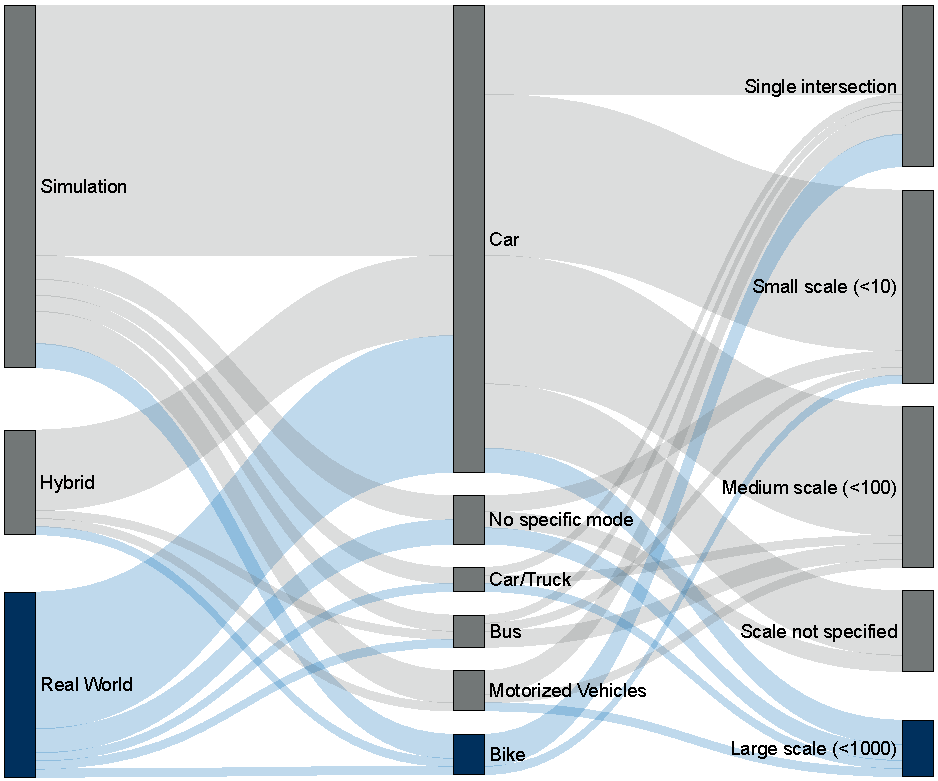
\includegraphics[width=\linewidth]{images/related-work-sankey.pdf}
\caption{Study environment, mode of transport, and number of intersections of related work on GLOSA. Aspects on which this study focuses are highlighted in blue.}
\label{fig:related-work-piechart}
\end{figure}

A key driver in research of GLOSA has been the studies by Audi and BMW, who, from 2008 to 2018, investigated GLOSA in real-world settings as part of their advanced driver assistance systems. In 2014, Protschky et al. \cite{protschky_extensive_2014, protschky_adaptive_2014} focused on a large-scale deployment in Munich, laying the methodological foundation for BMW's "EnLighten" app that was developed later by Wilson et al. (2017) \cite{wilson_driver_2017} and Sokolov et al. (2018) \cite{sokolov_effects_2018}. Both studies were conducted in the USA. In the project TRAVOLUTION (2008) \cite{braun_travolution-netzweite_2009}, Audi collaborated with the city of Ingolstadt and the German firm Gevas to lay the foundation for their own GLOSA system. The system design and the first results were published in 2013 by Zweck and Schuch \cite{zweck_traffic_2013}. By that time, Audi's GLOSA system included the cities of Verona, Garmisch, and Berlin, with a total number of over 700 intersection nodes. Later, in 2017, Stahlmann et al. \cite{stahlmann_multi-hop_2017} investigated options for Audi to directly obtain the traffic light data via short-range radio communication. Finally, in 2018, Stahlmann et al. \cite{stahlmann_exploring_2018} published a paper more broadly focusing on practical problems, finding that there are still unsolved challenges, even though development on GLOSA had proceeded for a decade at this point.

All of these studies have been tested in relatively extensive areas, enabled through the initiatives and pilots brought forward by car manufacturers in collaboration with cities. Apart from these studies, only a few works have investigated GLOSA on a similar scale. Khan et al. (2021) \cite{khan_eco-drive_2021} develop a cloud-based ECO-Driving system for the city of Ottawa with access to 1178 intersections. Bhattacharyya et al. (2022) \cite{bhattacharyya_assessing_2022} utilize data from a field-operational test in Bordeaux with access to 546 intersections. The work by Bhattacharyya et al. (2022) \cite{bhattacharyya_assessing_2022} is related to the mobile apps "CTD - Mobilité connectée"\footnote{\url{https://play.google.com/store/apps/details?id=com.geolocsystems.cthedifference}}, "CoopITS"\footnote{\url{https://play.google.com/store/apps/details?id=fr.gouv.developpementdurable.coopits}}, and work on the Cooperative Urban Mobility Portal\footnote{\url{https://co-ump.eu/data-samples-glosa/}} for Bordeaux. Two other commercial apps were developed in Germany: "TrafficPilot" (available in >10 German cities) by Gevas or "Signal2X" (available in Darmstadt) by Yunex \cite{yunex_traffic_v2x-kommunikation_2023}. Except these projects, most real-world GLOSA studies utilize a testbed with few turns, few traffic lights, and often a predefined route \cite{iglesias_i2v_2008, schweiger_elisatm_2011, raubitschek_predictive_2011, koukoumidis_signalguru_2011, koukoumidis_leveraging_2012, hao_eco-approach_2019, fickas_fast_2019, chen_developing_2022}. City-scale studies are still highly demanded to learn more about the applicability and benefits, but also potential drawbacks of GLOSA to real-world traffic.

Furthermore, research on GLOSA has been traditionally focused on car applications, and only a few studies have focused on transporting the progress in this domain over to cyclists. 

- Tal et al. (2016) \cite{tal_vehicular-communications-based_2016}: mobile system for e-bikes, evaluated in a hybridized simulation environment
- Dabiri et al. (2020) \cite{dabiri_optimized_2020}: optimized speed trajectories (simulation) based on different cyclist preference models -> coping with individuality of cyclists
- Halbach et al. (2021) \cite{halbach_cooperative_2021}: 


In simulations, Tal et al. (2016) \cite{tal_vehicular-communications-based_2016}, Dabiri et al. (2020) \cite{dabiri_optimized_2020} and Halbach et al. (2021) \cite{halbach_cooperative_2021} found that cyclists could expect similar improvements in ride comfortability and reduced energy expenditure due to lesser stopping.

The only real-world study of a GLOSA app for cyclists was conducted from 2018 to 2021 by Fickas and Schlossberg. The developed app, "FastTrack," was tested in 2019 on a small-scale test corridor (6 intersections) in Oregon \cite{fickas_fast_2019}. Auxiliary material on this study is available through the Portland State University online library \cite{fickas_green_2021, fickas_using_2021, fickas_riding_2019, fickas_data_2021, fickas_project_2018}. Apart from mobile apps like TrafficPilot that offer a cyclist mode besides their main application for cars, no other studies investigate GLOSA as a solution to motivate more people to cycle.

In the real world, static info boards were studied to inform cyclists about upcoming green phases \cite{lu_enhancement_2018}. 

In essence, this work aims to bridge the gap between GLOSA's current state -- largely concentrated on motorized vehicles -- and its potential application to a complete city network, with a spotlight on cyclists. The unique challenges posed by this expansive scope necessitate reevaluating established concepts and solutions, ensuring the development of a holistic GLOSA system.

\section{Challenges}

Apart from the general problem of the lack of focus on cyclists, the research domain surrounding GLOSA raises many interdisciplinary research issues: regulation and financing, integration and technology assessment, and possible consequences for society. This work focuses on the technical implementation of such a system and its assessment, resulting in four problems to address.

\addcontentsline{toc}{subsection}{Traffic Light Data for Prediction}
\textbf{\color{cidarkblue}Traffic Light Data for Prediction:} To provide a speed advisory for an upcoming traffic light, a prediction of the traffic light's switching behavior is required. The challenge lies in developing a robust system that is capable of seamlessly collecting real-time data from traffic lights across the city. This involves not only the integration of a data source but also the implementation of a prediction algorithm that can incorporate the recorded data and forecast the traffic light's behavior. Since a traffic light's switching behavior may depend highly on the current time and day, as well as the detected traffic density, a reliable and accurate prediction is challenging. Furthermore, there may be data outages or errors in the streamed data, which degrade the quality and trustworthiness of the prediction. Hence, achieving a highly accurate and trustworthy prediction is challenging but unquestionably paramount for the overall effectiveness of the speed advisory.

\addcontentsline{toc}{subsection}{Traffic Light Matching}
\textbf{\color{cidarkblue}Traffic Light Matching:} For which traffic light a speed advisory should be displayed depends on the user's planned trajectory across the next intersection(s). The extensive number of potential traffic lights across the city complicates the process, turning the identification of the matching traffic lights into a search for needles in the haystack. The system needs to efficiently and accurately pinpoint the relevant traffic lights that align with the user's route, considering factors such as distance and turn direction. The type of traffic traffic light is also important since cyclists occasionally share a traffic light with cars, buses, or pedestrians. The system should prefer dedicated traffic lights for cyclists whenever possible. Due to the often ambiguous choice in traffic lights at an intersection, the matching algorithm has to consider multiple variants and decide on the best traffic light. The challenge here lies not only in the algorithmic complexity of traffic light matching but also in ensuring real-time responsiveness to provide timely speed advisories.

\addcontentsline{toc}{subsection}{Accurate Bike Routing}
\textbf{\color{cidarkblue}Accurate Bike Routing:} To know which traffic lights will be along the way, this work will utilize a route-based approach for trajectory prediction and distance-to-signal estimation. This means that calculating a route accurately resembling bike trails is crucial for the speed advisory's accuracy. However, existing routing foundations are designed as general-purpose maps with a focus on motorists, meaning that bike paths are often missing or tagged inconsistently. One key focus of this work is, thus, to find methods that allow a more accurate bike routing to enhance the overall in-app experience and provide a solid foundation for an accurate speed advisory.

\addcontentsline{toc}{subsection}{Speed Advisory}
\textbf{\color{cidarkblue}Speed Advisory:} As cyclists navigate with the GLOSA app through the urban landscape, it becomes essential to tailor speed advisories to their individual needs and the context of their journey. This involves reducing cognitive load on the user as much as possible, allowing the cyclist to focus on the real-world situation. Maximizing the usefulness of the advisory system involves striking a balance between providing targeted speed advisories and avoiding unnecessary distractions. Factors such as the road's inclination, surface quality, and the type of bike being used are also crucial to determining the best route and speed advisory. Having solved these challenges, we can deploy the mobile application in a large-scale context and evaluate its impact. One major challenge is finding metrics that decrypt the recorded user data into meaningful insights about the impact of GLOSA on cycling behavior. A multifaceted approach is necessary to tackle this, encompassing quantitative and qualitative data. Understanding user perspectives is vital for ensuring that GLOSA aligns with user expectations and integrates seamlessly into their cycling routines. 

Together, these challenges represent the framework for this work to demystify the overarching question of how well the idea of GLOSA adapts to cyclists in a large-scale, real-world setting. By addressing one challenge by one, this study aims to draw potential repercussions and future work of implementing GLOSA for cyclists.

\section{How to Read This Thesis}

Having discussed the top-level structure and motivation of this work, the rest of this work is structured as follows. Each chapter follows one described challenge along the processing chain of a GLOSA system. First, in \Cref{ch:prediction}, we will discuss the challenge of traffic light prediction, contributing to the understanding of traffic light switching patterns and real-world deployment challenges, and obtaining a functional city-scale prediction system for our bike-GLOSA app. Afterward, in \Cref{ch:matching}, we connect the traffic light prediction with the cyclist by allowing the cyclist to match traffic lights along a preselected route. In \Cref{ch:routing}, we develop an accurate bike routing that improves traffic light matching and distance-to-signal estimation. The routing is integrated together with traffic light prediction and matching into the bike-GLOSA app in \Cref{ch:app}, focusing on the user interface to provide the best possible speed advisory. In this chapter, we also evaluate the impact of the speed advisory on cyclist behavior. 

Each chapter is self-contained and can also be read separately. In each chapter, a more challenge-specific introduction is given, delving into a report of current related work and observed research gaps. The described research gaps are described alongside methods to address these gaps. Finally, these methods are evaluated to draw conclusions and future avenues for research. Small summaries are given at the end of each section that provide all key points. At the end of this thesis, \Cref{ch:conclusions} summarizes the gained knowledge and main results for all individual challenges and gives an overarching outlook for future studies. 

  \chapter{Traffic Light Data for Prediction}\label{ch:prediction}

% TODO: Paper IV

\section{Introduction}

The fact that road users do not know when the traffic lights will change leads to several well-known problems. First, the issue of unneeded stopping and idling at red lights unnecessarily increases energy expenditure and emissions. In addition, not knowing about the upcoming traffic light's switching behavior also has negative impacts on road safety. There is a so-called dilemma zone when approaching a traffic light, where it unexpectedly turns yellow, and one must decide whether to stop before the light \cite{zhang_yellow_2014, suzuki_new_2018}. Often, this can lead to running a red light, speeding, or misunderstandings between drivers, increasing the overall risk of accidents.

Here, improved communication between vehicles and infrastructure elements could reduce the risk of accidents and traffic inefficiency \cite{sun_optimal_2020}. Such collaborative awareness is critical in current Cooperative Intelligent Transport Systems (C-ITS) research. Predicting traffic lights and communicating this prediction to vehicles, establishing the C-ITS day-1 service GLOSA, is one integral part of a more extensive portfolio of potential measures \cite{mellegard_day_2020}. Nonetheless, it is essential to consider that traffic light prediction is not strictly limited to GLOSA-like systems and may also lay the foundation for other application scenarios. For example, with the emergence of Augmented Reality, also in bike contexts \cite{matviienko_bikear_2022, kosch_notibike_2022}, there may be many more application scenarios than we currently envision.

Despite these encouraging prospects, traffic light prediction is currently associated with multiple challenges. Although countdown displays at traffic lights are widespread in various countries \cite{nygardhs_cyclists_2021}, integrating a mobile system to access and utilize the residual phase time directly from the traffic light's control unit presents a significant challenge. This process contrasts with the operation of countdown displays, which transfer the phase time internally to a countdown controller \cite{islam_improved_2016}.

A mobile system working across multiple intersections requires an interoperable data source. Here, the option exists to obtain the control programs directly, but without the current internal program state \cite{zweck_traffic_2013}. Since traffic-adaptive signals may only decide within a few seconds how long the next green phase will be switched \cite{islam_improved_2016}, this method is considered to be mainly restricted to fixed-time traffic light control programs that always switch in the same manner \cite{zweck_traffic_2013}. This is a strong limitation, as only 161 out of 1731 intersection controllers in Hamburg run a fixed-time program as of 2023\footnote{This information could be extracted from a traffic control inventory of the LSBG / IVS1 (as of June 22, 2023) provided on request, in addition to an inquiry to the Hamburg Senate: \url{https://www.buergerschaft-hh.de/parldok/dokument/72143/ampelschaltsysteme_gruene_welle.pdf}}. For the remaining 1570 traffic lights, we may expect interchanging or dynamic parts of the switching program.

Due to these issues, another method to access traffic light data has been established to deploy traffic light assistance services in the field. Most GLOSA applications use the residual time provided by Signal Phase and Timing (SPaT) messages generated on the intersection controller level and transmitted to the vehicle \cite{wagner_spatmap_2023}. However, such messages may only be available in some cases at the given location -- sometimes, as in this work, the prediction of traffic lights has to be performed purely by observing the outside state \cite{protschky_extensive_2014, protschky_adaptive_2014}. Furthermore, not all methods of traffic light data acquisition may be practical for smartphones.

In this work, we will utilize a centralized data broker, the Traffic Lights Data platform, that is provided by Hamburg authorities. However, a key challenge with these kinds of data platforms is the reliability of the traffic light data \cite{protschky_extensive_2014, protschky_adaptive_2014}. The state information may arrive incomplete, drop out completely for longer periods, or be highly delayed. These data issues impede the ability of the traffic light prediction to react to short-term changes in the program or may lead entirely to false and unavailable predictions. Quality assurance methods are required to identify these problems if they are present, and plan according solutions. This will be the first key challenge we will address in this chapter.

The second key challenge is the traffic-adaptiveness of traffic lights. Traffic-adaptive adjustments of switching programs are intended to improve the traffic flow at an intersection but have adverse effects on predictability due to short-term green time adjustments \cite{schweiger_elisatm_2011, bodenheimer_enabling_2014}. Recently, methods have been developed that focus on a more accurate prediction of traffic lights, but not all prediction methods may be equally suited for all kinds of traffic light patterns. Furthermore, some prediction methods may be more sensitive to data errors and outages than others. Thus, to understand precisely at which spot which prediction method is suited, the second main challenge of this chapter is developing a framework that helps in the decision process.

The goals of this chapter are to address these two challenges as follows. First, we will discuss the current methods to obtain traffic light data and which data issues may arise from centralized data infrastructures, as used in this work. Afterward, we will review state-of-the-art prediction methods and discuss their suitability for highly adaptive switching and highly erroneous data transmission. Based on this understanding, we will develop a twofold framework for traffic light data monitoring and data quality assurance. The first main component is monitoring methods that allow us to identify data issues and outages. Second, we develop metrics that can be used to measure the adaptivity patterns in traffic light switching and decide which kind of traffic light prediction may be suitable. Finally, we will evaluate the results of this framework and draw conclusions about how well traffic lights can be predicted in Hamburg with existing methods.

\section{Related Work}

To obtain a full picture of traffic light data and prediction, we will first look at studies designed to transmit traffic light data to traffic participants. These studies will provide a thorough understanding of the current data challenges behind GLOSA systems. Largely independent of these studies, multiple prediction methods that aim to improve prediction accuracy have been proposed. A discussion of these studies will help us learn the methods behind traffic light prediction and which issues may arise from a city-scale real-world deployment. Afterward, with the learnings from both domains, we will design a quality assurance framework for an existing data pipeline and prediction system in Hamburg.

\subsection{Data Challenges of Decentralized Systems}

In Europe, a large body of research and investments is currently flowing toward decentralized traffic light data systems, especially those based on Dedicated Short-Range Communication (DSRC). Road Side Units (RSUs) are deployed at intersections to operate these systems, sending standardized radio messages on the 5.9 GHz frequency band. These standardized C-ITS messages include SPaT messages, which vehicles can directly collect with a corresponding antenna (On Board Unit, OBU). A SPaT message contains the current switching state of a traffic light and a residual time until the next switch, making it an ideal data foundation for GLOSA applications \cite{ibrahim_estimating_2019, wagner_spatmap_2023}. Thus, many studies related to GLOSA utilize this data foundation \cite{schweiger_elisatm_2011, rakha_eco-driving_2011, rakha_aeris_2012, li_open_2012, suramardhana_driver-centric_2014, xu_bb_2015, bernais_design_2016, nguyen_efficient_2016, choudhury_integrated_2016, stahlmann_multi-hop_2017, stahlmann_exploring_2018, plianos_predictive_2018, zhang_green_2020, chen_developing_2022}.

SPaT messages are typically generated within the intersection controller level \cite{zweck_traffic_2013} and transmitted directly to an RSU without a centralized server system. However, such a system is typically not entirely decentralized. To calculate the residual time, there is the need for an additional prediction module, which may communicate with a cloud system in which a prediction algorithm is running \cite{strobl_c-its_2019, neuner_leitfaden_2020}. Due to the decentralized message transmission, however, a key advantage of this approach is that every vehicle equipped with a capable radio antenna has access to this data foundation. Thus, this approach is highly interoperable and attractive for manufacturers. The main per-unit cost factor is equipping intersections with the necessary RSUs \cite{niebel_cost-benefit-based_2013}.

A current research problem with decentralized approaches is the limited over-the-air radio transmission distance, especially when foliage blocks the line of sight. Since the 5.9 GHz frequency band resides closer to visible light's wavelength than other network carriers, such as 3G and 4G, it does not penetrate well through obstacles. In response to this issue, the C-Roads project, a prominent initiative in Europe's C-ITS landscape, submitted a statement advocating for the supplementation of the 5.9 GHz band with lower-frequency bands \cite{bohm_radio_2017}.

With DSRC only, Stahlmann et al. (2017) \cite{stahlmann_multi-hop_2017} show that obstacles may reduce the transmission range to less than 150 meters. The drop in the transmission rate is not immediate but gradual, which is why a partial message loss must always be assumed with this method. Sharara et al. (2019) \cite{sharara_impact_2019} provide more insights into the relation between packet loss, a GLOSA system's activation distance, and the speed advisory's effectiveness. The authors show that partial message loss of up to 90\% is not a significant problem unless the transmission distance is cut down too much, impacting the speed advisory system's activation distance and effectiveness. In a simulation with a minimum speed of 35 km/h, maximum speed of 75 km/h, specific green time of 25 seconds, red time of 40 seconds, and amber time of 5 seconds, Sharara et al. (2019) \cite{sharara_impact_2019} find that the transmission distance should be at least 850 meters for a 100\% success rate of traversing the green light, while 300 meters only resulted in 50\% -- 60\% of green passes depending on the message loss rate (90\% -- 10\%). Thus, with the transmission distance reported by Stahlmann et al. (2017) \cite{stahlmann_multi-hop_2017}, GLOSA services may occasionally fall short of their potential benefit simply because they are activated too late.

One explored solution to improve transmission range is an optimized RSU placement \cite{mehar_optimized_2015, massobrio_smart_2015, al-ezaly_optimal_2020}. Another option may be to adjust the transmission rate, which is reported in different ranges of 4 Hz \cite{stahlmann_multi-hop_2017} to 10 Hz in Hamburg \cite{stegen_ideas_2021}. The third option is inter-vehicle relaying of the messages to artificially expand the transmission range, as proposed by Stahlmann et al. (2017) \cite{stahlmann_multi-hop_2017}. Thus, a few practical solutions have already been presented to mitigate the limited transmission distance problem. For smartphone applications without direct access to an OBU, external antennas have been developed that can be connected via a USB cable \cite{kim_vulnerable_2017}. Additionally, manufacturers Bosch\footnote{\url{https://www.bosch-presse.de/pressportal/de/en/auto-cycling-and-tech-innovators-launch-coalition-for-cyclist-safety-based-on-v2x-deployments-259136.html}} and Canyon\footnote{\url{https://media-centre.canyon.com/en-INT/226588-canyon-plan-to-integrate-autotalks-v2x-technology-into-bicycles-to-help-reduce-accidents}} may introduce OBUs into their bike components soon, making this technology more accessible to cyclists.

One emerging alternative to 5.9 GHz radio is cellular vehicle-to-everything (V2X). This transmission technology utilizes an existing carrier medium such as 4G or 5G for the message transfer \cite{xia_field_2012, zweck_traffic_2013, bhattacharyya_assessing_2022}, distributing messages directly from an RSU (decentralized) \cite{bohm_radio_2017} or via cell towers (semi-decentralized) \cite{strobl_c-its_2019, jacob_ivs-kom_2020}. Although this carrier medium is interoperable on the application level (transmitting SPaT messages), there seem to be incompatibility issues on the network level \cite{bohm_radio_2017}. Thus, while DSRC is widely deployed on roads in Austria and Germany\footnote{\url{https://auto-talks.com/technology/dsrc-vs-c-v2x/}}, cellular V2X is seen by some experts to replace DSRC in the future\footnote{\url{https://www.cloudflight.io/en/blog/5g-killer-app-v2x-requires-the-transformation-the-automotive-industry/}}. Amid this uncertain state, C-ITS pilots \cite{strobl_c-its_2019} and OBU manufacturers \cite{jacob_ivs-kom_2020} develop multi-band solutions working with cellular V2X and DSRC in parallel.

Another issue is the unclear long-term compatibility of cellular V2X with smartphones. Not much research could be found in this direction, so we have to base our observation on technical documents. Although chipsets exist that enable LTE-V2X through the PC5 mode (direct device-to-device communication) and LTE-V2X/5G-V2X via cell towers\footnote{\url{https://5gaa.org/content/uploads/2021/11/5GAA_List_of_C_V2X_devices.pdf}}, these chipsets seem to be manufactured mainly for automotive applications. The 5G Automotive Association, a proponent of cellular V2X encompassing automotive and chipset manufacturers, predicted LTE-V2X in 2017 to penetrate 80\% of new smartphones by 2027\footnote{\url{https://5gaa.org/content/uploads/2017/12/5GAA-Road-safety-FINAL2017-12-05.pdf}}. However, this prediction is based on an optimistic scenario in which smartphone manufacturers react to increasing demand for C-ITS applications induced by LTE-V2X deployments in cars. There is also the pessimistic scenario in which 0\% of smartphones will support this technology in the future. Currently, it is up for speculation which scenario is more likely, meaning that cellular V2X is not yet an established data source for smartphone-based GLOSA applications.

\subsection{Data Challenges of Centralized Systems}

While DSRC and cellular V2X aim to provide a near-range network for C-ITS message communication, there is also the option for a traditional approach over the Internet. With this approach, the traffic light data is collected at a centralized server infrastructure located near the traffic management center and redistributed over an internet endpoint \cite{zweck_traffic_2013, protschky_extensive_2014, protschky_adaptive_2014}. In this way, a centralized traffic light data infrastructure circumvents two challenges of decentralized approaches: limited transmission range and long-term compatibility with smartphones. However, as we will see, it also shifts the responsibility of interoperability, data processing, and quality assurance toward the service consumer.

At Audi, Zweck et al. (2013) \cite{zweck_traffic_2013} established a data foundation for a GLOSA system that ingests traffic light data from three major cities. Correspondingly, three data adapters needed to be implemented: In Verona, the car manufacturer had access to SPaT messages generated on the intersection controller level. In Garmisch, intersection controllers were retrofitted with an additional SWARCO forecast module to obtain the necessary data, presumably SPaT messages. In Berlin, multiple traffic control centers were connected with various protocols, for which the specific transmission format is not further disclosed. The implemented data adapters were integrated into a centralized proprietary backend of Audi, making the corresponding traffic light information available to the company's vehicles via a mobile network connection to the internet. Unfortunately, the specific prediction methods and challenges related to traffic light prediction are not provided in detail. While it is generally unclear where this system is currently in operation, the available information indicates that the system was introduced in the United States in 2016 and was utilized at least until 2020 to facilitate Audi's GLOSA services in Düsseldorf \cite{neuner_leitfaden_2020}.

Many studies, whether decentralized or centralized, utilize the contained prediction in SPaT messages directly to generate the GLOSA service without needing an additional prediction system. In this way, these studies delegate the task of traffic light prediction to the infrastructure provider. However, some occasions may lead to the circumstance that the SPaT messages are not directly processable or available. The stability of the messages may also not be guaranteed at all times. Thus, it may be necessary to develop a custom prediction service that handles the available data formats and is robust to data outages, as shown by Protschky et al. (2014) \cite{protschky_extensive_2014, protschky_adaptive_2014}. In their studies conducted for BMW, the authors were confronted with multiple traffic light data issues in Munich. Usually, the delays in traffic light messages are within a few seconds \cite{neuner_leitfaden_2020}. However, in Munich, the authors had to work with SPaT messages arriving 10 to 60 minutes late from the city's data system. This significant delay meant that the residual prediction contained in the SPaT messages would be far outdated once the backend obtained this information. Furthermore, the traffic light messages were also partially incomplete.

Protschky et al. (2014) \cite{protschky_extensive_2014, protschky_adaptive_2014} approached the challenges as follows. First, they recorded the traffic light states contained in the SPaT messages, storing the data in histories for each traffic light. Afterward, they extrapolated the seen patterns in the historical data until the current time and slightly beyond to derive a prediction. In this way, the prediction was decoupled from the significant delays. When detecting that the prediction would no longer correlate with the actual observed data to over 95\% accuracy, as required by BMW, the prediction was turned off for the affected traffic lights. While the authors had to cope with significant data issues, their approach achieved a reported prediction availability of at least 69\%. Thus, while not all traffic lights could be predicted at all times, and the message delays likely imputed adaption to short-term changes in the traffic light behavior, the authors could still achieve a functional large-scale prediction system.

Compared to decentralized systems, centralized approaches to obtaining traffic light data are more compatible with smartphone applications and are still utilized today by at least one large car manufacturer. However, an ongoing challenge is to overcome the data issues of these systems. Protschky et al. (2014) \cite{protschky_extensive_2014, protschky_adaptive_2014} present a prediction method that even works when the data is highly delayed or incomplete. However, it must be expected that not all traffic lights will provide a prediction, as data errors may decrease the prediction availability.

\subsection{Traffic-Adaptive Signal Timing}

Due to the increased availability of traffic light data, it also becomes more viable to develop more intelligent coordination of the switching behavior at intersections. As shown by Wang et al. (2018) \cite{wang_review_2018}, a key research goal in traffic control is to develop more advanced coordination strategies for traffic lights, reducing unnecessary congestion. However, a more active traffic light control also means that passive assistance systems like GLOSA become more challenging. Thus, as discussed by Otto et al. (2023) \cite{otto_framework_2023}, both kinds of research actively work against each other. Different prediction approaches have been presented to counteract the issue of traffic adaptive signal timing for GLOSA systems. 

\begin{figure}[t]
\centering 
\begin{tabular}{ccc}
\footnotesize{(a) Fixed-time} & \footnotesize{(b) Partially adaptive} & \footnotesize{(c) Fully adaptive} \\
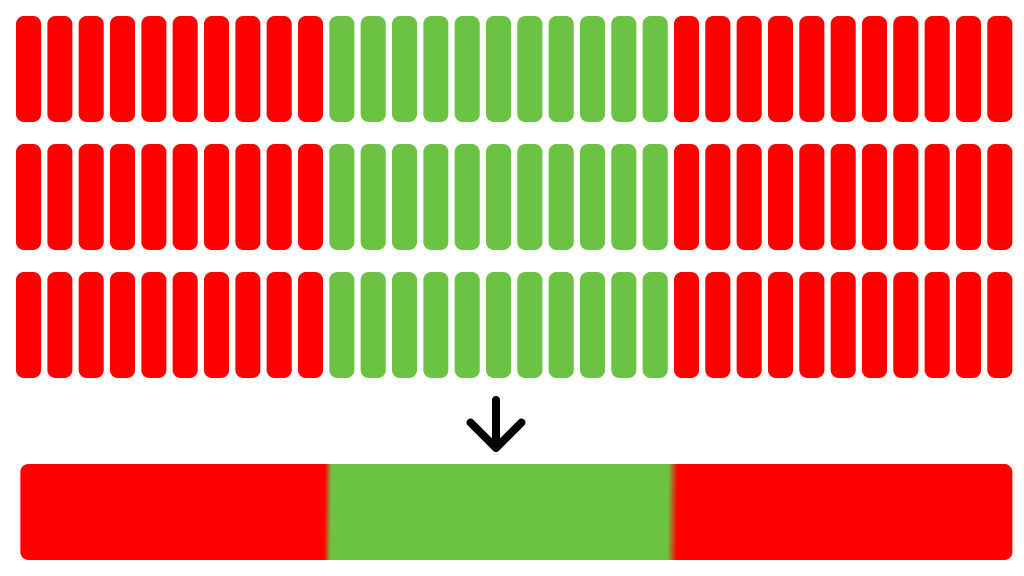
\includegraphics[width=0.3\linewidth]{images/explanation-fixed-time.png} & 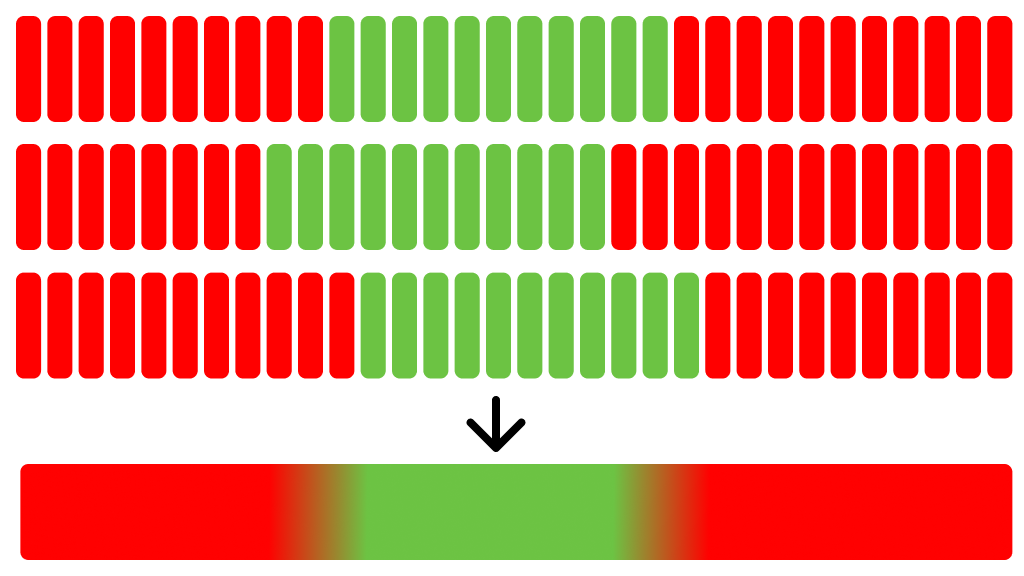
\includegraphics[width=0.3\linewidth]{images/explanation-partially-adaptive.png} & 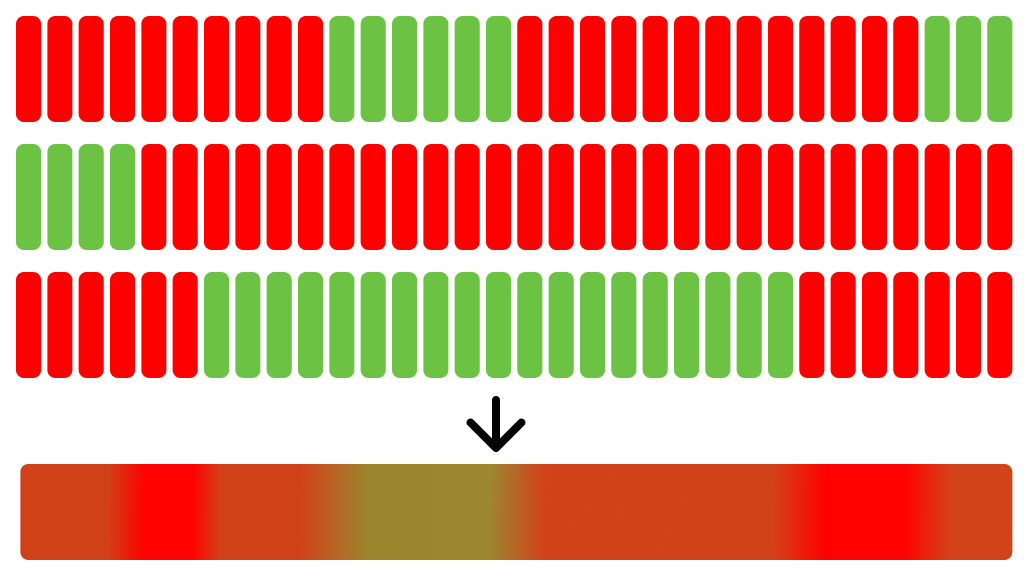
\includegraphics[width=0.3\linewidth]{images/explanation-fully-adaptive.png}
\end{tabular}
\caption{Taxonomy of the three types of traffic light adaptivity. Seen are the traffic light program cycles that contain the switched colors. On the bottom, we see a probabilistic prediction generated from the cycles and how the different types of adaptive switching behavior influence it.}
\label{fig:prediction}
\end{figure}

The first idea to address adaptive timing is to add probabilities to a traffic light prediction. With this approach, each second in the prediction is associated with a probability that the color will be seen at this moment, depending on previous switching behavior. This approach is illustrated in \Cref{fig:prediction}, and was initially proposed by Protschky et al. (2014) \cite{protschky_extensive_2014, protschky_adaptive_2014}. First, full circulations of the traffic light's program (cycles) are recorded and aligned in history. Alignment is performed with information on when a new cycle was started. Afterward, the probability of "green" and "red" is determined for each second through the prevalence of the predicted color at this specific second in previous cycles. Since the adaptive component is represented as a probability, the speed advisory can focus on certain parts of the prediction, counteracting the adaptive behavior. As a result, this kind of prediction algorithm reacts to traffic adaptive signal timing by blurring out uncertain parts of the prediction. 

With this approach, the speed advisory algorithm must decide which prediction parts are considered safe enough. One potential solution was introduced by Mahler et al. (2012) \cite{mahler_reducing_2012}, who showed possible optimization methods for calculating the optimal speed with an uncertain prediction. A recent work by Typaldos et al. (2023) \cite{typaldos_modified_2023} has further developed the idea of calculating a probabilistic/stochastic speed advisory. However, one intrinsic challenge of this approach is that, as adaptability increases, it tends to converge more towards the midpoint of the green phase. Following the speed recommendation may result in the vehicle not reaching the traffic light precisely on time but instead with some delay. Thus, from the standpoint of minimizing unnecessary braking as much as possible, the speed advisory is not necessarily "optimal."

Another idea explored in related works is to adjust the prediction in real-time to the observed traffic light states, stretching or shortening the predicted residual time when unpredicted changes happen. Such self-adaptive prediction methods have been initially proposed by Bodenheimer et al. (2014 -- 2015) \cite{bodenheimer_enabling_2014, bodenheimer_glosa_2015} through a graph-based method. Their method observes the ingress directions at an intersection node and reconstructs the relation between the clearance timing of each direction. Schneegans et al. (2023) \cite{schneegans_prediction_2023} also demonstrate the possibility of utilizing Machine Learning models for this process. Here, the idea is to utilize a sequence prediction model trained on prerecorded timing data from a specific traffic light. In general, self-adaptive methods, and especially methods based on sequence prediction, seem to be a recent trend in achieving higher accuracy, following the success of Machine Learning in other domains.

However, self-adaptive methods are not without criticism. As pointed out by Stahlmann et al. (2018) \cite{stahlmann_exploring_2018}, the stretching and shortening of the prediction can also be seen as a significant disadvantage of this approach. Since repeated adjustments to the prediction during the intersection approach may negatively impact usability, there is a clear tradeoff between the prediction's accuracy and temporal stability. The increased computational complexity of the presented Machine Learning models is also a factor that may negatively impact the prediction algorithm's scalability toward multiple thousand traffic lights. There is currently no evidence supporting the scalability on a large scale as opposed to probabilistic approaches \cite{protschky_extensive_2014, protschky_adaptive_2014}. 

Furthermore, while the probabilistic approach is intrinsically robust to incomplete data and can drop individual cycles, error robustness is another factor to consider in evaluating self-adaptive models. These challenges must be addressed to employ such a model in practice. Most importantly, however, the traffic light data must arrive in time for the self-adaption to happen. Thus, self-adaptive prediction methods can only be employed when the traffic light data arrives with low latency, posing a significant limitation for real-world deployments. In a situation such as reported by Protschky et al. (2014) \cite{protschky_extensive_2014, protschky_adaptive_2014} where traffic light messages may arrive with a delay of over 10 minutes, a self-adaption would be basically useless.

In general, the issue of traffic adaptivity is not fully solved yet, with limitations in both probabilistic and self-adaptive prediction methods. However, the necessity to address this issue also depends on the extent to which traffic adaptivity is actually present in the real world. Here, various reports can be found.

Cai et al. (2009) \cite{cai_adaptive_2009} were the first to report that "most" traffic lights in their context are traffic-adaptive. Concrete numbers were presented by Bodenheimer et al. (2014) \cite{bodenheimer_enabling_2014}, who reported that 95\% of traffic lights in Hamburg were adaptive and 73\% in the ten largest German cities. Fakler et al. (2014) \cite{fakler_structures_2014} also found a high proportion of traffic-actuated control systems in German cities with over 50000 inhabitants. Schneegans et al. (2022) \cite{scheegans_exploiting_2022} and Heckmann et al. (2023) \cite{heckmann_stage_2023} further support the conclusion that most traffic lights are operated by traffic-adaptive controls. Hao et al. (2019) \cite{hao_eco-approach_2019} noted the widespread deployment of actuated traffic light controllers in the US, while Avatefipour and Sadry (2019) \cite{avatefipour_traffic_2018} found that fixed timing is more prevalent in Malaysia. Grumert and Pereira (2022) \cite{grumert_heads-up_2022} found that 70\% of traffic lights in Sweden are adaptive. Thus, there seem to be regional differences in the implementation.

Unfortunately, we found no global studies based on reliable sources that investigate the employment of traffic light adaptivity by country. Only one study by Olaverri-Monreal et al. (2018) \cite{olaverri-monreal_implementation_2018} could be found that did not clearly refer to a specific region. The authors report that adaptive timing is only implemented in a small number of road networks, and the majority of urban areas still use pre-timed control systems. However, how reliable this information can be considered is not fully clear, as a source for this finding was not provided. A similar issue also applies to other studies. For example, in the work by Bodenheimer et al. (2014) \cite{bodenheimer_enabling_2014}, which mentions 95\% adaptive traffic lights in Hamburg, it was only clarified upon inquiry that these results were based on a survey conducted by a service provider on behalf of Audi. The study by Grumert and Pereira (2022) \cite{grumert_heads-up_2022} provides a Swedish source for their findings, but we were unable to find it. Hence, we have to be intrinsically skeptical about these reports.

Based on the information we have, Germany seems to utilize traffic-adaptive signals predominantly. Findings for Hamburg roughly align with our analysis that counted 90.7\% (1570 out of 1731) adaptivity-capable traffic light controllers. However, aside from the general lack of verifiable results, the implications for predictability remain largely unexplored. While the capacity to adapt to traffic may exist, it might be underutilized or manifested only in minor adjustments, potentially resulting in a less significant impact on prediction accuracy, as indicated by the reported percentages. Presently, no study examines the real-world effects of adaptiveness on predictability, leaving a significant research gap.

\begin{Summary}[Summary of Research Gap]
While many works focus on decentralized data transmission, a centralized approach is currently the best option for cyclist applications. Most centralized platforms provide an endpoint for SPaT messages generated at the intersection controller level. Based on this endpoint, the residual time prediction in SPaT messages can be directly used for a speed advisory application.

In cases where no SPaT messages are available or arrive too late, the best approach involves recording switching histories, running a suitable prediction algorithm on these histories, and sending the generated predictions to service users. Data latencies can be circumvented through an appropriate prediction approach, such as a probabilistic method. Nonetheless, there are only few works on the data challenges on a larger scale, thus requiring more research. Existing works indicate significant issues with data reliability that must be accounted for.

Furthermore, it is unclear at which intersections novel prediction methods such as machine learning models may provide a better prediction than the existing probabilistic method. Although machine learning methods may have advantages and provide a more self-adaptive prediction, issues like unproven robustness against data errors, scalability, and the temporal instability of the predicted residual time mean that we have to carefully consider at which crossings these methods should be applied. 

While some studies pose traffic-adaptive switching behavior as their central motivation to develop more advanced prediction methods, it is unclear how justified these motivations are. Reported numbers of adaptive traffic lights provide a rough estimate but no definite conclusion about the actual predictability of traffic lights. If adaptiveness is seen but is limited to a few seconds, it may necessitate reevaluation of developed prediction algorithms. Here, a direct analysis of traffic light data is needed to determine how many traffic lights exhibit adaptive behavior and how much this behavior impacts predictability.
\end{Summary}

\section{Concept}

We will conduct two steps to address the described research gaps. First, we will design a quality assurance framework that monitors data availability and potential errors, at the example of our traffic light data infrastructure in Hamburg. The goal is to provide quality assurance solutions to improve the prediction that GLOSA app users can expect as much as possible. Using a monitoring infrastructure, we will conduct a large-scale, long-term study on the prediction availability and quality. As a prediction method, we reuse the existing probabilistic prediction method, with the goal of identifying potential weaknesses and advantages of that method in our field deployment and how reliable traffic light data is.

Second, we address the need for more research on traffic light adaptiveness and predictability. In contrast to previous studies, we attempt to measure the predictability directly, and identify which kinds of prediction algorithm may be applicable at each intersection. To conduct such a study, we first collect large amounts of traffic light data. Afterward, we design and evaluate two novel metrics that help us measure which kinds of prediction methods may be applicable. The goal is to provide the first large-scale insights into the kinds of traffic light patterns that are seen in a large city such as Hamburg and thus clarify how much traffic adaptivity is a concern for traffic light prediction.

\subsection{Data Quality Assurance}

To bring forward intelligent transport solutions such as GLOSA applications, Hamburg employs an open data policy through its self-imposed transparency law (HmbTG\footnote{\url{https://transparenz.hamburg.de/gesetzestext-des-hmbtg-636070}}), providing several kinds of urban data free of charge to the public. Hamburg provides static, continuously updated, real-time datasets and geo APIs as part of this urban data platform. One of these APIs is the Traffic Lights Data\footnote{\url{https://metaver.de/trefferanzeige?docuuid=AB32CF78-389A-4579-9C5E-867EF31CA225}} system, which provides real-time information about the switching of traffic lights in Hamburg and georeferences their location in the city. Published by the Free and Hanseatic City of Hamburg, Landesbetrieb Straßen, Brücken und Gewässer (LSBG), the data is made available under the DL-DE BY-2.0\footnote{\url{https://www.govdata.de/dl-de/by-2-0}} license and will be considered the foundation of this work.

One challenge of using the Traffic Lights Data platform for prediction and speed advisory in a GLOSA application is that the state messages are not provided in the SPaT format. Thus, no residual time prediction, as contained in SPaT messages, is available, meaning that we have to implement an external prediction service to establish our GLOSA service. Changes in each traffic light's state are provided as real-time observations through the SensorThings\footnote{\url{https://www.ogc.org/standard/sensorthings/}} "Observation" format. Besides vehicle detector or bus request messages, three particular types of messages represent the foundation for our prediction:

\begin{itemize}
    \item \textbf{(Primary) signal color}: the current traffic light color and the time when this color was switched. Among green, red, amber, and amber-red, there are also other specific states such as amber-flashing, green-flashing, or dark (light turned off). The color is given for the primary signal head and supplementary signals, such as green arrows.
    \item \textbf{Signal program}: the current program ID running on the traffic light, with a time when this program was switched.
    \item \textbf{Cycle second}: a timestamp indicating that program recirculation has happened. With this timing information, the continuous stream of colors can be split into cycles, usually 90, 75, or 60 seconds long. This information is also given for traffic lights that do not strictly use a circulating program routine.
\end{itemize}

The Traffic Lights Data platform was designed based on an existing traffic controller infrastructure and implemented by various stakeholders. The system design of the platform follows these technical and organizational constraints, resulting in a rather complex chain of information. As we will later see, precisely understanding this chain of information is crucial to tracing data issues that may arise. Thus, through dialogues with various authorities in Hamburg, we reconstructed a precise picture of the infrastructure and potential points of failure.

\begin{figure}[t]
\centering
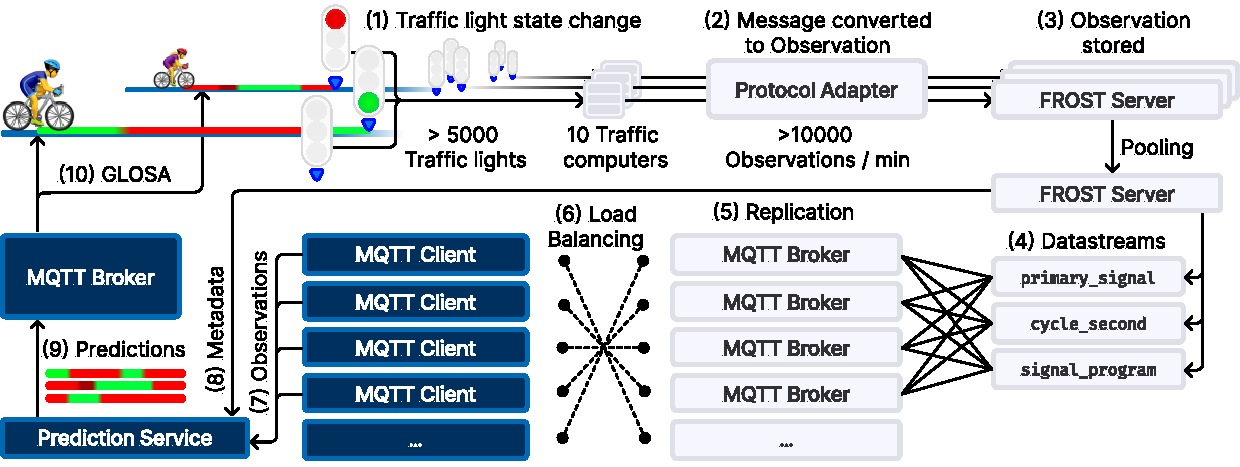
\includegraphics[width=\linewidth]{images/traffic-light-data-infrastructure.pdf}
\caption{Data flow diagram of the existing traffic light data infrastructure. Highlighted in grey are the components of the Traffic Lights Data infrastructure. Blue components highlight our implemented data adapter and prediction services.}
\label{fig:traffic-light-data-infrastructure}
\end{figure}

To provide state messages in the Traffic Lights Data platform, they are translated and shifted multiple times between various data brokers. First, as seen in \Cref{fig:traffic-light-data-infrastructure}, the state messages are sent in a controller-specific format to one of ten traffic controllers (1). Then, the messages are converted to Observations (2) and sent to a corresponding SensorThings server. From there, a centralized SensorThings server collects all Observations (3), which are associated with a specific type of "Datastream" encapsulating the type of Observation: \texttt{primary\_signal} (color), \texttt{cycle\_second}, and \texttt{signal\_program} (4). Finally, the messages are published across an autoscaled Kubernetes cluster of MQTT brokers (5). 

Afterward, our prediction service connects to the broker endpoint to ingest all Observation messages. Our prediction service utilizes multiple MQTT clients with individual TCP connections to balance the load on each MQTT broker in the Traffic Lights Data platform (6). The collected Observations (7) are combined, knowing which Observation is associated with which traffic light through metadata in the Traffic Lights Data platform (8). This metadata allows the prediction service to record a history of program cycles and associate it with the corresponding traffic light ID. Based on these histories that are continuously updated, the prediction algorithm runs periodically to keep predictions up to date (9). 

The prediction algorithm itself was implemented by Sebastian Pape based on the method developed in his Diploma thesis \cite{pape_untersuchung_2012} and integrated into the data pipeline with corresponding programming interfaces. The programming interface converts the Observations into an internal format for the prediction algorithm, meaning that the programming interface is interoperable with other message formats as long as the three described types of traffic light state messages are given. Based on this foundation, the developed service could be seamlessly ported to other cities that provide the desired messages.

At its foundation, the integrated prediction method is equivalent to the probabilistic method by Protschky et al. (2014) \cite{protschky_extensive_2014, protschky_adaptive_2014}. It reconstructs cycles based on the cycle timing information and calculates which color will most likely appear for each second. To allow the prediction algorithm to adapt to changing programs, only the last ten cycles are kept for prediction. Then, every 60 seconds, the current history of each traffic light is fetched, and a new prediction is calculated based on the current time. The prediction is extrapolated to be 180 seconds long. This extrapolation will allow our app to display an appropriate speed advisory even when users are far from the traffic light. Afterward, the generated prediction is published on an MQTT broker under the traffic light's ID, where the app is subscribed and automatically obtains new information. The prediction MQTT broker is configured to retain all messages, meaning that a new app subscription directly sends the last prediction for the subscribed traffic light. Finally, the app utilizes the obtained prediction to display a speed advisory.

\begin{figure}[t]
\centering
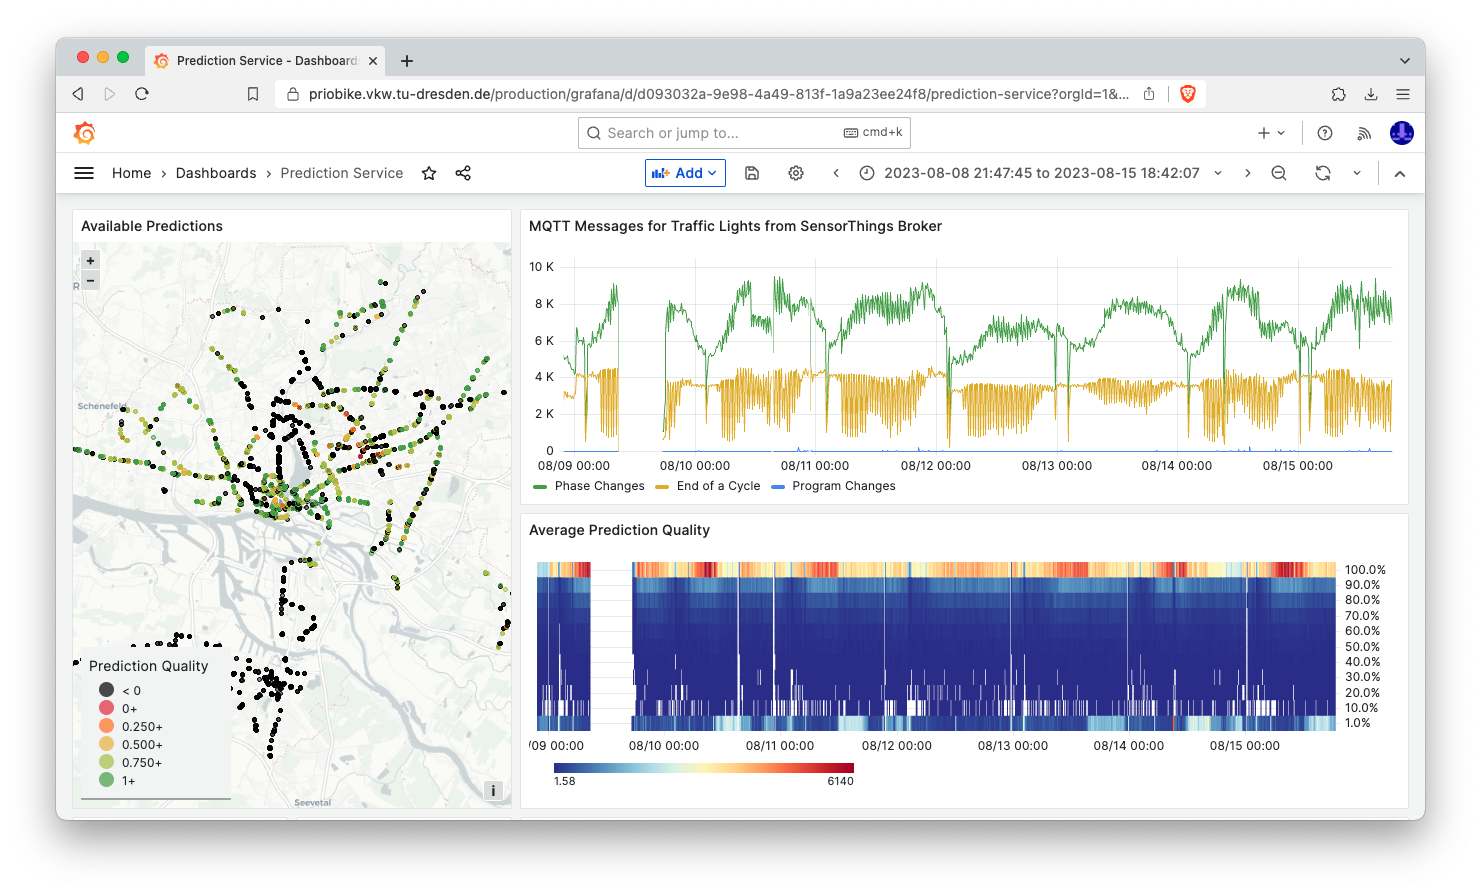
\includegraphics[width=\linewidth]{images/monitoring-screenshot.png}
\caption{Screenshot of the developed monitoring solution. Within the Grafana dashboard, three key aspects of data quality can be observed: the number of messages (top right), the distribution of prediction quality (bottom right), and the quality of predictions throughout the city (left).}
\label{fig:monitoring-screenshot}
\end{figure}

A monitoring solution was developed to supervise whether the data infrastructure and the prediction algorithm work as intended. This solution, shown in \Cref{fig:monitoring-screenshot}, is based on a web dashboard that highlights real-time metrics such as the number of Observations, generated predictions, and spatial distribution of the measured prediction qualities. 

We also measure the number of invalid cycles, referring to cycles that contain invalid transitions between traffic light phases. Specifically, we check if a recorded cycle deviates from the regular switching patterns red--red-amber--green--amber and red--green. We check the length of amber against its maximum duration of 6 seconds, together with the maximum red-amber duration of 2 seconds, as specified by German traffic light operation constraints \cite{TN_libero_mab2}. Detected erroneous cycles are then discarded by the prediction service and logged by the monitoring system to identify outbreaks of erroneous data.

The developed monitoring allows us to identify and report data failures to the platform operators based on discarded erroneous cycles, drops in the number of Observation messages, or a decreased prediction quality. Error patterns in the dropped messages allow us to provide more detailed information about the potential origins of data failures within the system's architecture.

Here, the prediction quality is calculated as follows. After creating a new prediction vector $P$, it is held for 120 seconds. Then, each second in the collected data vector $D$ is compared to the prediction $P$, calculating an accuracy score:


\begin{equation} 
\text{Prediction Quality}(D, P) = 
\frac{
\sum_{i=0}^{119} 
\left\{
\begin{array}{ll}
1 & \text{if } D[i] = P[i] \\
0 & \text{otherwise}
\end{array} 
\right.
}{
120
}
\end{equation}\label{eq:predictionquality}

Note that $D$ is not part of $P$, meaning the prediction is validated on unseen data. The calculated quality is then attached to the newly generated prediction, and the time when the quality was created is noted. If we have no real-time data, no quality is calculated. This means that, in the case of a data outage, the quality is not refreshed. After 10 minutes, when the quality cannot be refreshed, it is set to -1 to indicate that validation is no longer possible. Based on this information, we can also see when a data outage occurs or when the traffic light turns itself off.

By viewing the prediction quality on a map, especially qualities mapped to -1, we can directly identify whether an outage is related to a specific traffic controller or associated with the complete city. If all city districts are affected, the problem is more likely to originate from the data pooling or load balancing components further along the information chain. Furthermore, we can study the time and duration of error patterns, giving us and the system's operators more clues about where to look for data issues. Finally, we deploy one additional monitoring instance at an external cloud provider to cross out issues from our TU Dresden deployment.

\subsection{Predictability Metrics}

Based on the same data pipeline, we conduct our predictability analysis. However, instead of collecting the data to generate predictions, we use it to measure the absence or presence of predictable patterns. To achieve this distinction, the idea is to measure how "noisy" the switching patterns are. The more random noise is seen in the switching behavior, the less predictable the traffic light.

Until we arrived at our final metrics, we investigated various methods from other disciplines to measure noisiness. For example, one idea was to measure the Shannon entropy of the traffic light's data stream, indicating how much information content and, thus, complexity of the switching behavior is present. Similarly, we attempted to use compression techniques to find how much information content is in the traffic light program. Another idea was to utilize a fast Fourier transform to find how many different frequencies in the switching patterns were present, mapping states between green (1) and red (0)\footnote{A future avenue of this approach could be to employ other methods for period detection in the switching patterns \cite{breitenbach_method_2023}. Such an approach was not tested as part of this work.}. However, in the end, none of the attempted methods yielded a satisfactory measurement of how many predictable patterns were present while comparing the calculated values against case studies. 

Based on the learnings from these methods, we approached the challenge with two more direct measurements that each indicate one simple kind of unpredictability. The first metric is based on the difference between recorded cycles. If there were traffic light colors that appeared at different times in the cycles, this would directly indicate a kind of traffic adaption. We gave this metric the name cycle discrepancy, calculated between two recorded cycles $C_1$ and $C_2$ each, with the lengths $l_1$ and $l_2$:

\begin{equation} \text{Cycle Discrepancy}(C_1, C_2) =  \sum_{i=0}^{\max(l_1, l_2)-1} \left\{
\begin{array}{ll}
1 & \text{if } i \geq l_1 \text{ or } i \geq l_2 \\
1 & \text{if } C_1[i] \neq C_2[i] \\
0 & \text{otherwise}
\end{array} \right.\end{equation}

The cycle discrepancy is zero in cases when colors perfectly align between cycles, and cycles have the same length. However, for example, if the green phase in one cycle appears and ends one second earlier than in the last cycle, the cycle discrepancy is calculated at two seconds. Thus, the more shift is seen between two cycles, the higher our cycle discrepancy. When a high discrepancy between two cycles is seen, this also indicates a high traffic adaptivity in the switching behavior. Note also the similarity to \Cref{eq:predictionquality}, which is intentional.

The cycle discrepancy assumes that green phases are aligned with the cycle length, meaning they appear at the same time every cycle. However, there may also be traffic lights where the waiting time between green phases is not aligned with the cycle timing. While the waiting time could be consistent and, thus, predictable, the cycle discrepancy would be high due to the misalignment. Hence, we designed a second metric that captures how many different wait times are seen. If all waiting times differ, this also indicates a high traffic adaptivity without being bound to the cycle length.

We name this metric the wait time diversity and calculate it as follows. First, the recorded cycles are concatenated into a continuous history $H_{C_1, \dots, C_n}$ of traffic light switching. Then, between every two green phases for which a continuous record is present, the wait time in between is measured and rounded in seconds. As a result, we obtain a list of wait times between green phases. Then, we measure how many \textit{different} waiting times are seen proportionally to the number of all wait times:

\begin{equation}
\text{Wait Time Diversity}(H_{C_1, \dots, C_n}) = \frac{\text{\# Different Wait Times}}{\text{\# Total Wait Times}}
\end{equation}

If there are reoccurring green patterns in the wait time, the wait time diversity is expected to be close to zero. If the variability of waiting times between green phases is high, and thus the number of different wait times, the wait time diversity is expected to be close to one. In the extreme case that only one green phase is detected, the metric is set to one, meaning no reoccurring pattern was detected. If no green phase is detected, the metric is set to zero, assuming this represents an easily predictable pattern (always red).

Since the wait time diversity does not necessarily capture the amount of shift between green phases and only the uniqueness, both measures need to be employed in conjunction to determine whether predictable patterns are present.

\definecolor{good}{HTML}{00bb00}
\definecolor{bad}{HTML}{ff0000}
\begin{table}[!b]
\centering
\def\arraystretch{1.5}
\caption{Types of predictability mapped by our two metrics. This schema can be utilized to determine which kind of prediction algorithm may be suitable.}
\label{tab:cases}
\begin{tabular}{c|c|c|}
\multicolumn{1}{c}{} & \multicolumn{2}{c}{Cycle Discrepancy} \\
\cline{2-3}
Wait Time Diversity& Low& High\\
\hline
\multicolumn{1}{|c|}{High}& \textbf{\color{good} High predictability}$^1$& \textbf{\color{bad} Low predictability} \\
\hline
\multicolumn{1}{|c|}{Low}& \textbf{\color{good} High predictability}& \textbf{\color{good} High predictability}$^2$\\
\hline
\multicolumn{3}{l}{$^1$\footnotesize{Unpredictable wait time between green phases.}} \\
\multicolumn{3}{l}{$^2$\footnotesize{Unpredictable with our cycle-stacking (probabilistic) prediction method.}}
\end{tabular}
\end{table}

As a result, we obtain a measurement model that focuses on four cases, as visible in \Cref{tab:cases}. Whenever both measurements are low (bottom-left), the predictability is likely high with any of the currently available prediction methods, as each cycle tends to match with the next one, and the times between green phases also revolve. Similarly, when both measurements are high (top-right), the traffic light is likely poorly predictable, likely exhibiting highly spontaneous switching behavior. 

A more differentiated evaluation is necessary in cases where only one of both metrics is high. High cycle discrepancy in the presence of a low wait time diversity (bottom-right) indicates that our selected probabilistic prediction method should be avoided. It indicates that cycles are offset or non-matching, meaning that a cycle-stacking prediction algorithm will encounter intense blurring of the predicted colors. 

On the other hand, if the cycle discrepancy is low and the wait time diversity is high (top-left), the wait time between green phases is not well predictable, while cycles are similar. This may be the case when the traffic light only occasionally switches to green and shows red for the longest time. In this case, predicting red would be an accurate prediction in almost all cases, even though a green phase may occur at some point.

To apply this set of metrics to the traffic light data in Hamburg, we reuse the same data infrastructure as proposed earlier. However, we apply minor modifications to obtain more reliable measurements. As an additional error detection metric, we filter out all cycles that are 50\% longer or shorter than the previously recorded cycle length. This error metric aims to avoid too long or too short cycles skewing the final measurement, as they would boost the cycle discrepancy metric.

We also aim to minimize the noted problem of dropped Observation messages from the MQTT streams. Since the completeness of the messages is more critical for our predictability study than their timeliness, we can apply a workaround to get many more Observations than possible with MQTT only. We query all Datastreams in a round-robin fashion via the HTTP interface of the Traffic Lights Data API and fetch the latest Observations via this web interface. If we encounter any unseen Observations, we insert them into the database in which our MQTT Observations are located. 

Although theoretically applicable to the prediction service, this process is likely not an option for supplementing the real-time data during the traffic light prediction. Browsing through data streams via the HTTP interface takes a few minutes per roundtrip, meaning we would have to delay our MQTT Observations or adjust the reconstructed cycles artificially, which was not seen as sensible with the given algorithm implementation, although theoretically viable. Therefore, this approach was only applied in the data recording phase, which does not rely on sequential and minimally delayed Observations. Not integrating the complex HTTP queries into our prediction service also means the Traffic Lights Data platform does not have to deal with a continued disproportionate load after our experiment is finished.

During our experiment, the recorded data of all traffic lights is stored in a Postgres database. However, due to the large number of messages obtained, we also employ some optimizations to the data storing and database fetching process. During analysis, we group the received data into hourly buckets, each representing one hour recorded for the specific traffic light in the weekly turnus. Data from multiple weeks is overlayed onto the same hourly buckets. This process allows for efficient fetching of the billions of database rows and gives us a weekly progression of both predictability metrics for each traffic light, completing our concept for predictability analysis.

\begin{Summary}[Summary of Concept]
The designed prediction infrastructure makes use of Hamburg's centralized Traffic Lights Data platform and integrates an existing probabilistic prediction method  \cite{pape_untersuchung_2012} that follows the same cycle-stacking approach as proposed by Protschky et al. (2014) \cite{protschky_extensive_2014, protschky_adaptive_2014}. We chose this method as it guarantees high scalability and robustness to latencies and data errors. Interoperability with other cities is given whenever traffic light color, program, and cycle second information is available.

Focusing on data quality assurance, erroneous patterns like deviations from the regular switching order are detected, and associated cycles are discarded. This error cleanup method is based on the resilience of the cycle-stacking method to data gaps. Finally, we conceive a monitoring system to help identify and fix potential systematic issues in the traffic light data infrastructure in a dialogue process with Hamburg's authorities. We conduct a long-term study of the prediction availability, quality, and scalability achieved based on the recorded monitoring metrics.

In addition to our monitoring system, we also conduct a predictability analysis of the traffic lights in Hamburg. This predictability analysis reuses the established traffic light data infrastructure to record and analyze traffic light cycles. A direct measurement of the observed switching patterns provides a more explicit view of the predictability than was given in previous studies. The impact of adaptiveness on predictability is measured with two metrics: the cycle discrepancy, incorporating the per-second difference between traffic light cycles, and the wait time diversity, which measures the uniqueness of wait times between green phases. Predictability can be considered high if both metrics are low for a given traffic light. If only one metric is low, the predictability is also high, but not all prediction methods may apply.
\end{Summary}

\section{Results}

The evaluation of the prediction infrastructure is divided into two parts: assessing the prediction process and evaluating traffic light predictability in Hamburg.

First, we examine how well the prediction system interacts with the Traffic Lights Data platform and identify potential weaknesses. Our examination involves analyzing traffic light predictions' spatial coverage and trends over an extended period, utilizing recorded metrics from the implemented monitoring system. We investigate the temporal availability of predictions to understand the number of traffic lights in Hamburg where speed recommendations can be expected. 

To identify potentials where our availability could be improved, we examine the recorded metrics from the implemented monitoring tool, identifying recurring error patterns that suggest systematic issues in Hamburg's data infrastructure. Collaborating with the data platform operators, we find the root causes of data outages and propose potential solutions. To further demonstrate the scalability of the prediction algorithm, we briefly examine the CPU, RAM, and network usage of the prediction service.

The second part of the evaluation focuses on our study of traffic light predictability in Hamburg. Based on related work and our inquiry to Hamburg's authorities, we expect at least 90.7\% of traffic lights to be capable of traffic adaptiveness. By analyzing the predictability metrics throughout the week and their distributions across Hamburg, we cross-check this value and analyze how well Hamburg is generally suited for a GLOSA system.

\subsection{Long-Term Data and Prediction Study}

As seen in \Cref{tab:tld-number-of-things}, as of December 2023, the Traffic Lights Data system contains 19951 individual traffic lights distributed across 791 intersection nodes, based on their ID that contains the intersection number. The system's overall number of traffic lights gradually changes as new ones are added or outdated entries are removed. Compared to our inquiry that referenced 1731 individual intersection controllers in total, 45.7\% of Hamburg is supported in December 2023. In this calculation, we assume that each intersection number is related to one individual intersection controller. Thus, 45.7\% represents a rough estimate, as there may be intersections with multiple controllers or, vice versa, controllers that manage multiple adjacent intersections.

\begin{table}[t]
    \centering
    \begin{tabular}{@{}lcccccccccr@{}}
        \toprule
        \textbf{Lane Type} & \multicolumn{9}{c}{\textbf{Tag from Metadata in Traffic Lights Data Platform}} & \textbf{$\Sigma$} \\
        \midrule
        Car        & $\times$ & $\times$ & $\times$ &   &   & $\times$ &   &   &   &  9649 \\
        Bus        &   &   & $\times$ &   &   & $\times$ & $\times$ &   & $\times$ &  1309 \\
        Bike     & $\times$ &   & $\times$ & $\times$ &   &   &   & $\times$ & $\times$ &  5477 \\
        Pedestrian &   &   &   &   & $\times$ &   &   & $\times$ &   &  6408 \\
        \midrule
        $\Sigma$ (unique) & 1509 & 7077 & 217 & 3646 & 6315 & 846 & 234 & 93 & 12 & \\
        \bottomrule
    \end{tabular}
    \caption{Number of individual traffic lights in the Traffic Lights Data platform as of December 4, 2023. Some traffic lights are marked for shared usage between multiple modes of transport, leading to overlaps in the numbers on the right side. The necessary metadata is provided by authorities in Hamburg.}
    \label{tab:tld-number-of-things}
\end{table}

Two minor errors in the metadata were identified during a preliminary examination of traffic lights. First, one of the traffic lights (132\_22) exhibited a duplicated \texttt{cycle\_second} data stream. Additionally, \texttt{laneType} "16371" was mistakenly assigned to traffic lights 240\_1 and 240\_2. These are not included in \Cref{tab:tld-number-of-things} as they cannot be accurately assigned. Both issues were traced back to human data input errors through communication with operators, and corrective measures could be initiated.

Out of the 19951 traffic lights, 5477 are designated for use by cyclists and were thus included for prediction. These numbers include mixed usage with public transportation, pedestrians, and cars. Recorded data for these traffic lights, measured from December 4, 2022 to December 4, 2023, show an average of 8532 \texttt{primary\_signal} Observations, 3318 \texttt{cycle\_second} Observations, and 27.7 \texttt{program\_change} Observations per minute received and processed via MQTT. During this time, the prediction service was offline for 75 hours due to planned maintenance or technical issues and online for 8680 hours, resulting in a calculated 99.14\% uptime. For 5 hours, the status is unclear as the entire VM or only the monitoring was offline. Assuming 80 hours of downtime, we have a 99.08\% uptime. Therefore, it should be noted when interpreting the following metrics that not 100\% of the period is covered.

\begin{figure}[t]
    \centering
    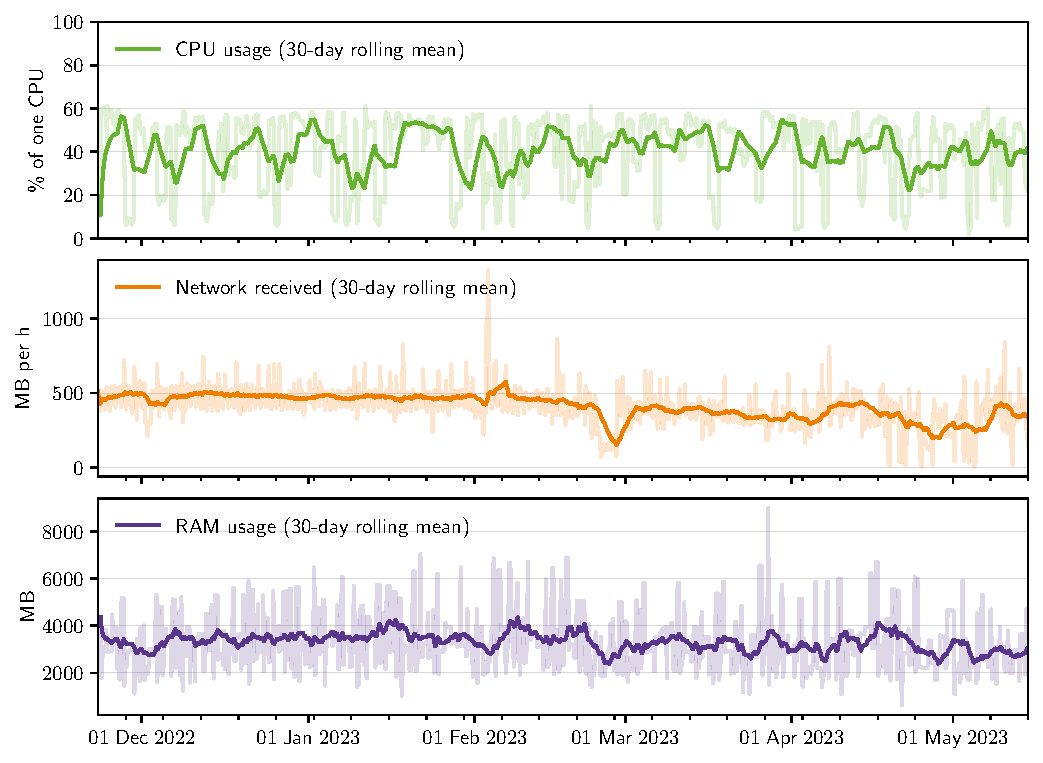
\includegraphics[width=\linewidth]{images/monitoring-prediction-service-load.pdf}
    \caption{Cadvisor statistics for prediction service. Seen here is that the load metrics of the prediction service are within acceptable limits when running the prediction for real-time data of approximately 5000 bike traffic lights.}\label{fig:monitoring-prediction-service-load}
\end{figure}

Based on collected Cadvisor\footnote{\url{https://github.com/google/cadvisor}} metrics on CPU load, RAM usage, and network load, the prediction algorithm scaled well to the multiple thousand traffic lights. The algorithm was implemented in a Java service that also controlled receiving Observations and sending Predictions to our prediction MQTT broker. We measured the service on a TU Dresden server using 6 of 12 cores of an Intel Xeon Gold 6136 CPU running at 3.00 GHz. The CPU percentage utilization of the prediction service was measured via CPU time. As seen in \Cref{fig:monitoring-prediction-service-load}, the service consumes approximately 60\% of the CPU time of a single CPU, translating to around 10\% of the total possible computing capacity when considering the 6 CPUs available on our VM. Both network usage and RAM consumption did also not exceed the capabilities of our VM, meaning that the resource usage was quite low considering the number of messages that were processed every minute.

\begin{figure}[t]
    \centering
    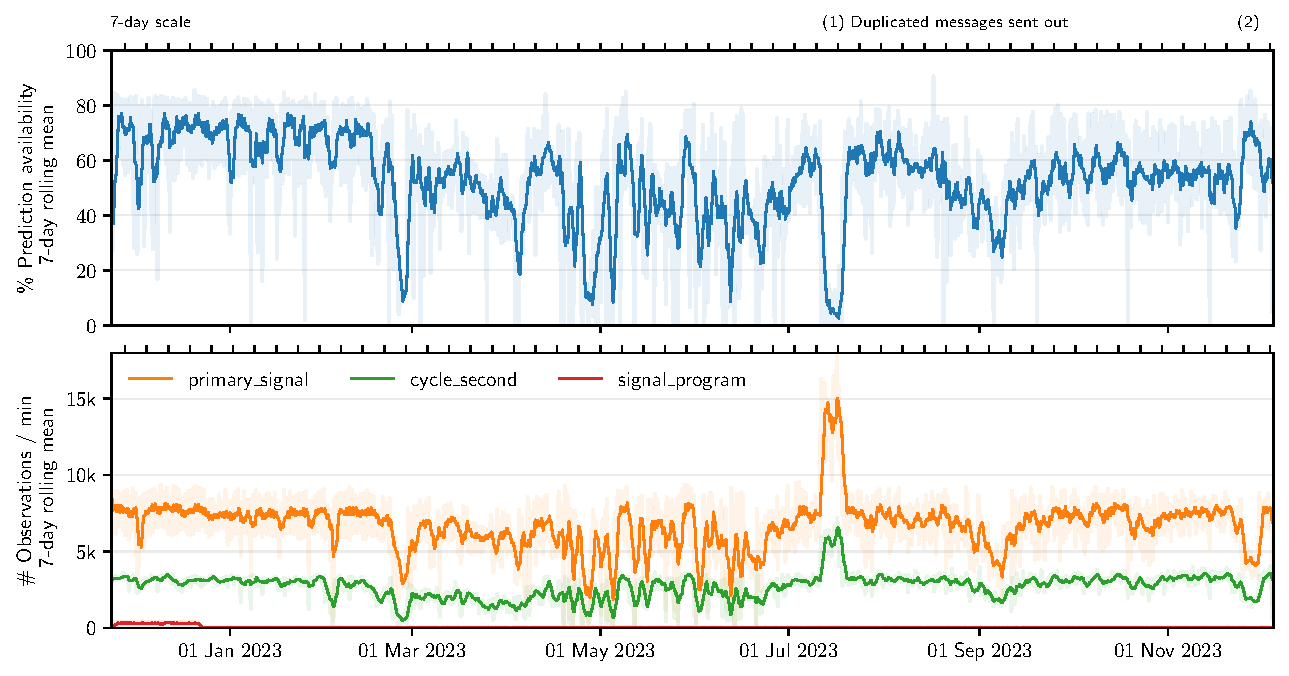
\includegraphics[width=\linewidth]{images/monitoring-availability.pdf}
    \caption{Long-term development of prediction availability. Shown here is for how many traffic lights a prediction was available during 2023, and how drops in availability directly relate to data outages or errors.}\label{fig:monitoring-availability}
\end{figure}

Following this aspect, the long-term data trend and prediction availability are depicted in \Cref{fig:monitoring-availability}. The prediction availability is calculated by dividing the number of predictions generated per minute by the total number of available traffic lights. In the upper part of the figure, we observe that prediction availability typically fluctuates between 40\% and 80\%, with 100\% never being reached. For the period given in the diagram, we calculate a median prediction availability of 55.07\% (IQR: 28.23\%). The maximum observed prediction availability resides at 90.63\%, recorded on September 17, 2023, at 0:00. Thus, the median prediction availability is relatively low throughout the studied period, lower than the minimum of 69\% reported by Protschky et al. (2014) \cite{protschky_extensive_2014, protschky_adaptive_2014} in Munich, while some weeks showed good service availability.

The visible disruptions in prediction availability can be primarily attributed to short-term data errors in the Traffic Lights Data system. For instance, around July 11, 2023 (1), all Observations were accidentally sent twice, causing prediction availability to nearly drop to 0\%. Examining the long-term trend, we notice increased disruptions in prediction availability in the summer of 2023, following an initial period of relatively stable availability. These disruptions coincided with increased maintenance activities on the Traffic Lights Data system, indicating that repeated updates during this period led to a deterioration in data quality. 

Although an increase in prediction availability can be seen around November 23, 2023 (2), this increase originated from us excluding erroneous traffic lights from our prediction service, decreasing the overall number of Observations received. Therefore, the prediction availability over the period under consideration was not optimal.

\begin{figure}[t]
    \centering
    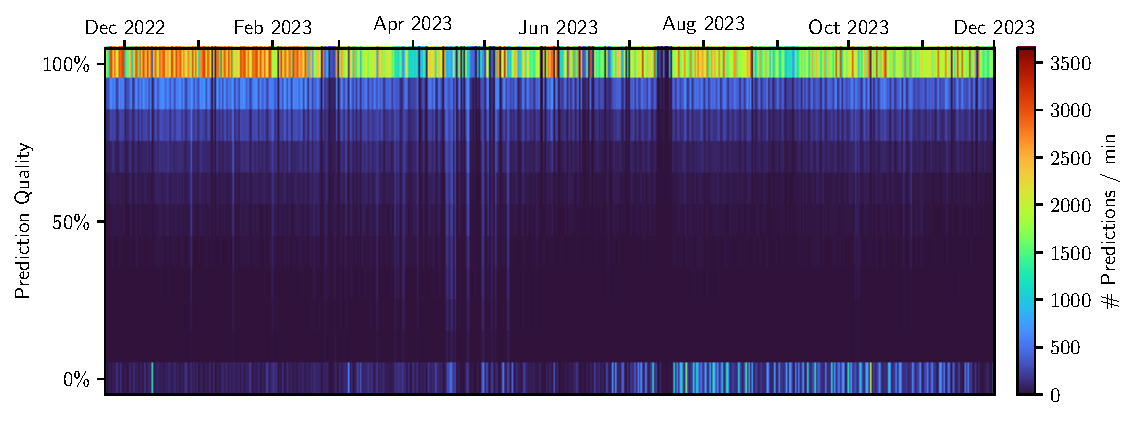
\includegraphics[width=\linewidth]{images/monitoring-long-term-study.pdf}
    \caption{A heatmap displaying the long-term development of prediction quality throughout 2023. The prediction quality was recorded in 10\% buckets for a more responsive analysis in our monitoring tool. In the best case, all predictions should be in the top 10\% bucket. Seen here is how data outages in late 2023 degraded the prediction quality.}\label{fig:monitoring-long-term-study}
\end{figure}

In addition to the prediction availability, we also measured the prediction quality over a longer period. \Cref{fig:monitoring-long-term-study} shows this measurement, mapping prediction qualities of -1 that indicate data outages to the 0\% bucket. 

Considering the 10\% buckets in which the prediction quality was monitored, the calculated median prediction quality resides at 85.78\% (IQR: 1.85\%). At first glance, examining the long-term trend reveals a similar pattern in prediction availability at 100\% quality compared to \Cref{fig:monitoring-availability}. For example, there was also a significant dip around July 11, 2023, due to the duplicated messages issue and a general decrease in availability throughout 2023. In addition, we can see in this diagram that fewer predictions fall within the intermediate 10\% to 90\% quality range. As the increased data outages in the summer of 2023 coincided with an increase in low-quality predictions, most predictions below 10\% are likely due to temporarily missing data. Thus, if interpreted as an accuracy metric, many predictions generated with consistent traffic light data likely have been precise to a few seconds.

\begin{figure}[t]
    \centering
    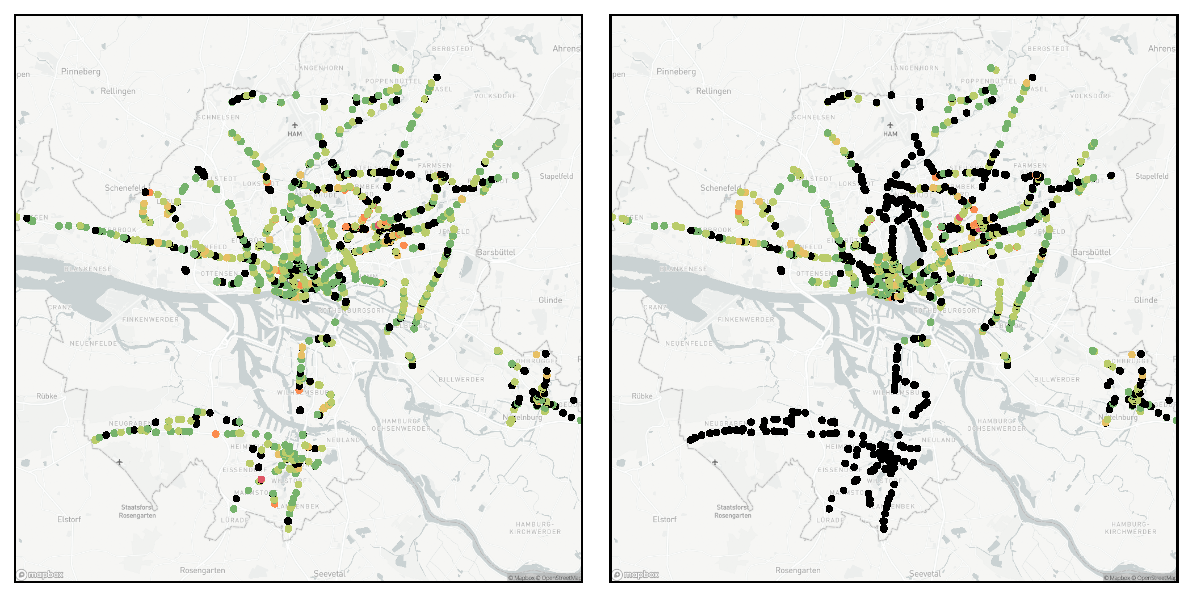
\includegraphics[width=\linewidth]{images/monitoring-before-after-failure.pdf}
    \caption{Before and after traffic controller failure on October 11, 2023. Black predictions indicate outages when the prediction service is unable to verify the prediction quality due to the lack of real-time data. In this case, entire city districts were affected by the outage, pointing to a systematic issue.}\label{fig:monitoring-before-after-failure}
\end{figure}

The decline in prediction availability observed in the summer of 2023 has had multiple origins, many of which could be identified, reported, and addressed through our monitoring tools. The first two kinds of data error that could be pinpointed are highlighted in  \Cref{fig:monitoring-before-after-failure}: blackouts of individual traffic lights (on the left and right) and blackouts affecting entire city districts (on the right only).

Through our map-based prediction quality monitoring, we could help identify 61 intersections and 80 individual connections experiencing persistent issues, rendering them unable to transmit data. In at least 30 cases, a connection was falsely associated with an unsignaled road crossing, or the connection was no longer present. Among 22 nodes, traffic lights utilized the OCIT protocol, which is unsupported by the Traffic Lights Data platform at the time of writing. For 19 nodes, the observed failures are presumed to be construction-related, with this confirmed in three additional cases. In 16 instances, outdated intersection topologies or georeferences were identified. The identified traffic lights were subsequently excluded from the prediction system using an exclude list, with the option to reintegrate them later.

Turning our attention to failures affecting entire city districts, \Cref{fig:monitoring-failure} demonstrates their relatively spontaneous occurrence. This type of failure poses a more significant challenge than individual intersection or connection failures since thousands of predictions are abruptly invalidated. Therefore, we worked rigorously with the platform operators to identify the source of this issue.

\begin{figure}[t]
    \centering
    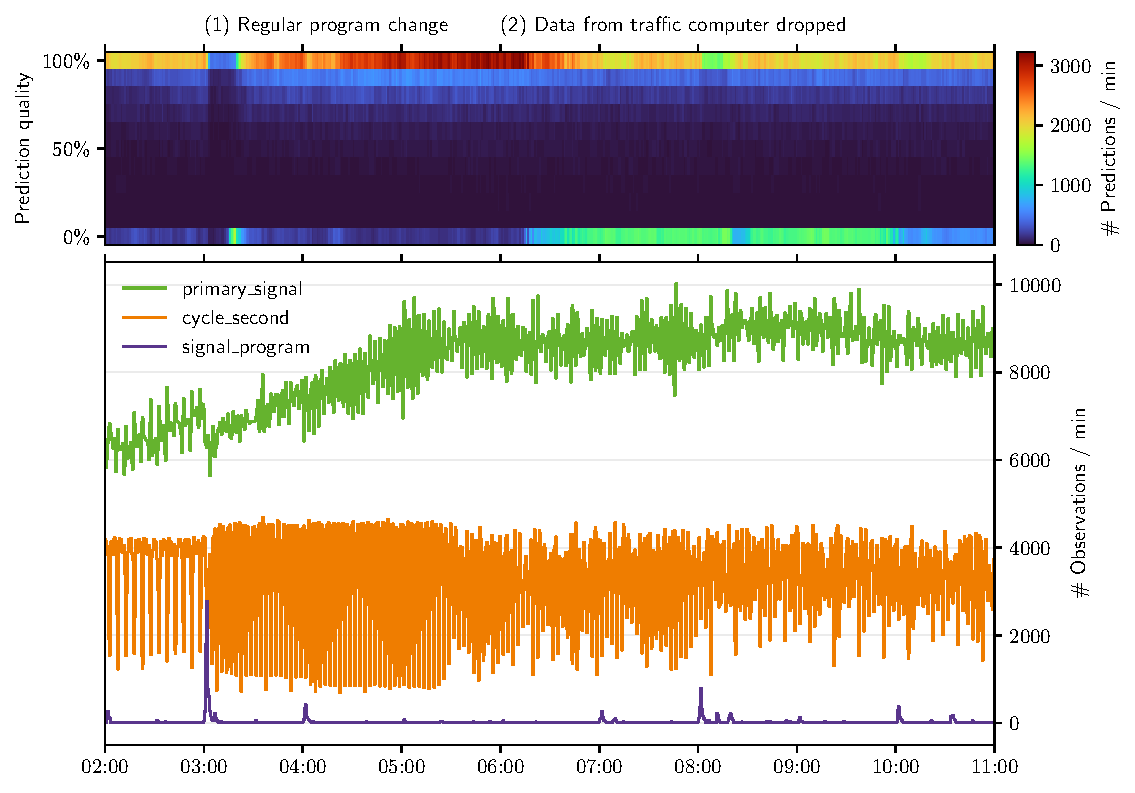
\includegraphics[width=\linewidth]{images/monitoring-failure.pdf}
    \caption{Monitored metrics during traffic controller failure on October 11, 2023. Seen on the bottom are typical patterns of real-time state messages that arrive at the prediction service. Here, no specific issue can be seen. However, the prediction quality heatmap shows a rapid decline in prediction quality that persists for multiple hours. This failure is related to \Cref{fig:monitoring-before-after-failure}.}\label{fig:monitoring-failure}
\end{figure}

To better understand the occurrence of such a failure, we examined the daily data course recorded by our monitoring system, as depicted in \Cref{fig:monitoring-failure}. At 3:00 AM UTC, within the timeline of \texttt{signal\_program} Observations, many traffic lights switch their programs. As confirmed by traffic light operators, this pattern represents the morning program of the weekly automation of the traffic lights being scheduled.

Simultaneously, the availability and quality of the predictions briefly decline (1). This decline can be explained by the fact that the prediction algorithm continues to forecast the old pattern from the previous program for a short period, only synchronizing with the new program after approximately 15 minutes (or ten cycles at 90 seconds). The reason is that the prediction service continues to record cycles and pushes out older cycles from the prediction window only after a few minutes. One identified solution for this issue is to switch between histories recorded for each traffic light once a program Observation arrives.

Following this brief decline, the best prediction quality is achieved around 6:00 AM UTC, just before it suddenly and persistently collapses across multiple districts. The fact that these declines are reflected in specific districts strongly suggests that this issue can be traced back to specific traffic controllers, each generating Observations for one or more districts. 

Once this finding was communicated to the Traffic Lights Data platform operators, it was identified that this problem is indeed associated with specific traffic controllers. The increasing message load throughout the day due to rising traffic causes the message queues of the MQTT brokers at the traffic controllers to fill up. Ultimately, this results in the traffic controllers either not sending messages at all, dropping individual messages, or transmitting them with significant delays.

\begin{figure}[t]
    \centering
    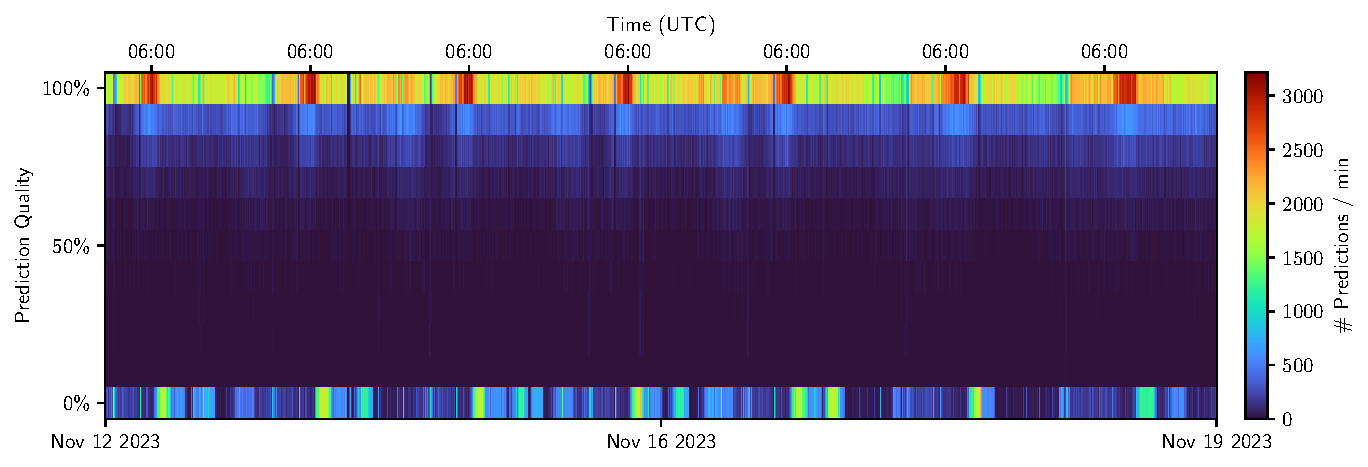
\includegraphics[width=\linewidth]{images/monitoring-7-days.pdf}
    \caption{Heatmap depicting the reoccurring nature of the traffic controller failures after 6:00 UTC. Each time a failure happens, we can see a clear decline in prediction quality, filling up the 0\% bucket.}\label{fig:monitoring-7-days}
\end{figure}

In the weekly progression illustrated in \Cref{fig:monitoring-7-days}, it becomes evident that this situation repeated almost daily at the same hour. Only on Saturdays and Sundays does the issue manifest later, around 7:00 -- 8:00 AM UTC, due to reduced and delayed traffic leading to fewer green phases.

Upon identifying the root cause, the operators initiated appropriate fixes related to the traffic controllers' MQTT queues. Simultaneously, we created an additional exclusion list of intersection nodes, preliminarily exempting them from the prediction until the issue was resolved. This exclusion involved 584 intersections connected to three specific traffic controllers. Due to compliance concerns, the operators have not allowed us to disclose the specific traffic controllers affected; however, further information can be found in a technical report from 2020 \cite{neuner_leitfaden_2020}. 

\begin{figure}[t]
    \centering
    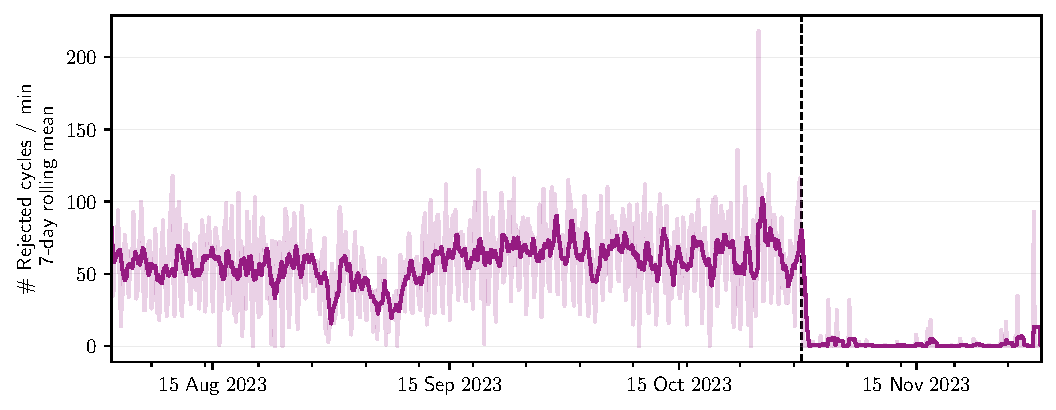
\includegraphics[width=\linewidth]{images/monitoring-rejected-cycles.pdf}
    \caption{Line chart depicting the number of cycles rejected due to out-of-order switching. The clear decline after October 31 at 6:40 AM local time indicates that parts of the traffic light data network infrastructure were fixed, decreasing the number of incomplete cycles.}\label{fig:monitoring-rejected-cycles}
\end{figure}

Looking at the number of discarded cycles, we derive further insights into whether isolated messages are lost or if Observations from operational traffic lights consistently reach their destination. The analysis is depicted in \Cref{fig:monitoring-rejected-cycles} and started around August 1, 2023. After an extended period with invalid cycles, we see a substantial improvement around October 31 at 6:40 AM local time. The number of rejected cycles suddenly dropped to 0, with only sporadic peaks. This improvement indicates that another data issue in the Traffic Lights Data platform was addressed; however, we were not informed which specific modification was made. Before, 25 to 125 cycles were rejected every minute, indicating that the issue could have affected up to 200 connections throughout summer 2023, assuming a cycle length of 90 seconds. At the time of this fix, we had already given Hamburg guest access to our monitoring web tool, meaning it could have been one of the information sources involved in the fix.

After identifying issues with the traffic controllers and falsely importing traffic lights in the data platform, we were also able to identify issues related to the network router installed at the platform operator's servers, which could not keep up with all messages. The corresponding router was replaced, further improving the data quality. The stability of the MQTT brokers directly connected with the traffic controllers was also optimized by scaling up the computational resources of the Observation-exporting virtual machines. As a result of these efforts, the original prediction availability from 2022 (80\% during the day) could be restored in February 2024, stabilizing the Traffic Lights Data system.

\subsection{Study of Traffic Light Predictability in Hamburg}

In the previous section, we found that the prediction availability for traffic lights in Hamburg was low during 2023. However, the core part of this issue could be attributed to data issues. The prediction quality was also likely affected by data issues, as predictions would be invalidated by the missing data, resulting in a prediction quality of -1 (no validation possible) mapped to 0\% in the monitoring. We found that the remaining predictions were mainly centered on 90\% to 100\% quality, more than we expected with the high prevalence of adaptivity-capable traffic lights in Hamburg. This finding was also a key motivation for further investigating the overall predictability of traffic light patterns. 

To conduct these evaluations, we recorded real-time data for four weeks. This recording encompassed 19844 individual traffic lights available in the Traffic Lights Data system at the time of evaluation, including all modes of transport and not only cyclist traffic lights, as in the previous study. During the measurement period, data was obtained from 18009 (90.75\%) of all traffic lights, among which 519 also contained secondary signal data. Thus, although we supplemented the MQTT messages browsing Observations from the Traffic Lights Data platform's HTTP interface, some traffic lights never sent data.

Nonetheless, the supplementation was still effective in addressing partial data outages, as seen in \Cref{fig:adaptiveness-mqtt-http}. On multiple days, approximately half of all recorded Observations were supplemented by the HTTP interface because they were lost preliminarily via MQTT. A minor message dip remained for some days, meaning small parts could not be recovered.


\begin{figure}[t]
    \centering
    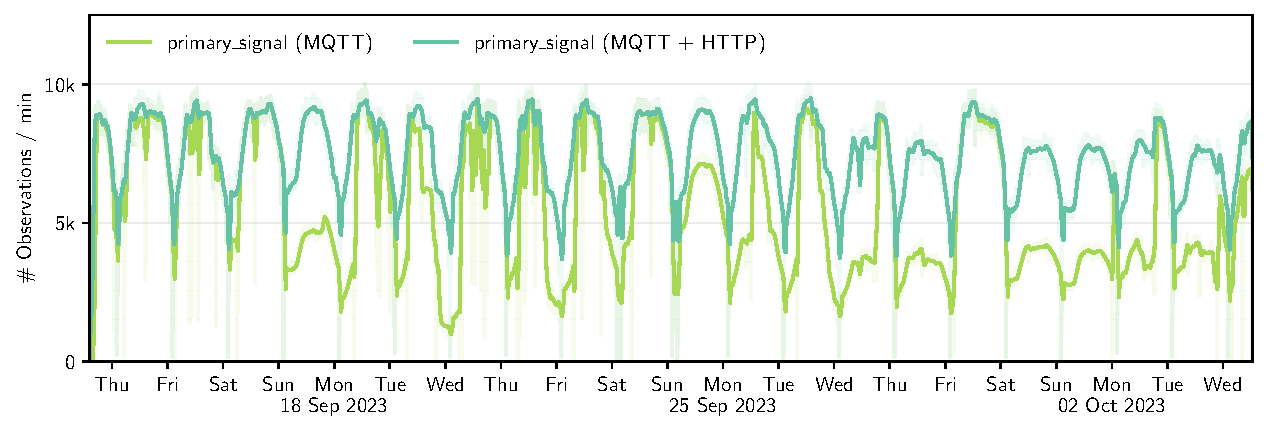
\includegraphics[width=\linewidth]{images/adaptiveness-mqtt-http.pdf}
    \caption{Line chart depicting how many messages were supplemented by browsing through the Traffic Light Data platform's HTTP API, recovering messages that were lost via MQTT.}\label{fig:adaptiveness-mqtt-http}
\end{figure}

The detection of faulty cycles, also implemented in the prediction service, was utilized for problem identification. Out of approximately 424 million reconstructed cycles, 13.8 million cycles were discarded. Here, 90\% of faulty cycles are distributed across 10\% of the connections. One of the known faulty traffic controllers could be identified as the leading cause by examining the faulty connections on the map\footnote{Unfortunately, we cannot disclose the specific traffic controller here due to compliance concerns of authorities in Hamburg, although we would have wished to do so.}. 

These numbers are related to the 40\% of traffic lights that were detected to switch between green, (red-)amber, and red. 34\% of traffic lights that only switched between green and red could also have generated erroneous cycles that were not discarded. The remaining 26\% of traffic lights are comprised of various other switching patterns. The 2106 traffic lights for which an error rate of >10\% was detected were excluded from further analyses.

\begin{figure}[!t]
    \centering
    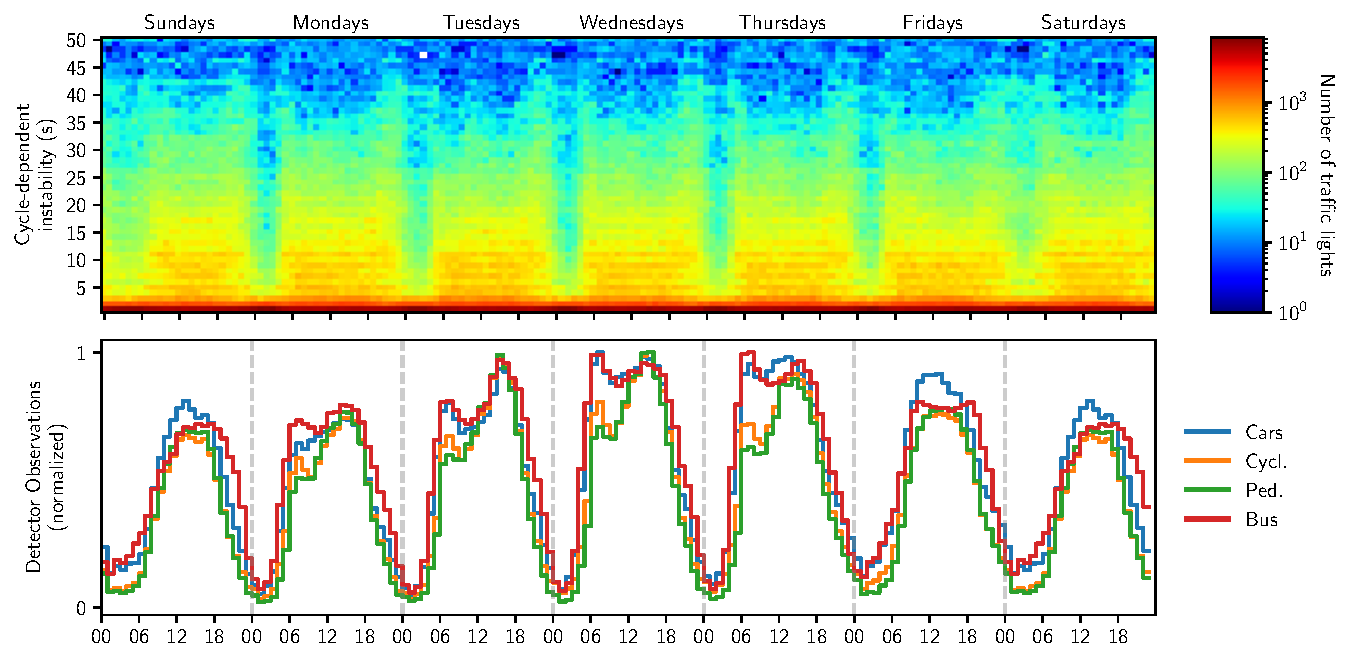
\includegraphics[width=\linewidth]{images/predictability-week-heatmap.pdf}
    \caption{Measured weekly progression of our two predictability metrics, cycle discrepancy and wait time diversity, in relation to the green length and the number of measured green phases throughout the day and the measured traffic volume from vehicle detector Observations. A higher number of vehicle detector Observations indicates a higher traffic density.}\label{fig:adaptiveness-weekdays-distance}
\end{figure}

Thus, we could not eliminate all errors, but they are present only to a minor extent. We assume that the mass of valid data overshadows isolated recording errors. However, it is important to note for subsequent analyses that recording errors may have occurred, e.g., missing cycle Observations leading to multiplied cycle lengths. Accordingly, we will use statistics for evaluation that are robust to outliers.

The first chart displayed in \Cref{fig:adaptiveness-weekdays-distance} looks at the relation between traffic light predictability and daytime. As a statistically robust measure against outliers in the data, we use the median of the cycle discrepancy and wait time diversity for all recorded hourly buckets to analyze how unpredictability evolves during the day. The information and the frequencies of recorded traffic detector Observations are presented to compare the measured predictability to the measured traffic volume.

As a result, predictability decreases, as expected, with increasing traffic volume. While the predictability is at its highest at night, it declines rapidly during the morning traffic surge. This is visible through the increased values in cycle discrepancy and wait time diversity in the heatmap. After the decrease in predictability, it remains relatively constant before increasing again in the evening. It looks like the predictability hits a lower bound, indicating that there may be limits to the adaptiveness even with further increasing traffic. 

When looking closer at the distribution and not only the general trend, the biggest part of traffic lights by one order of magnitude seem not to be influenced by adaptivity at all. As a result, across all traffic lights, the median cycle discrepancy ranges only between 0 and 2 seconds, depending on daytime. The highest median cycle discrepancy during the day comprises only 10\% of the median green length measured at 20 to 23 seconds, meaning that green phases largely overlap between cycles. The wait time diversity shows a similar pattern, although the number of traffic lights with 100\% wait time diversity increases during nighttime. This increase is likely because traffic lights switch to fewer green phases, increasing the chance that the waiting time between green phases is unique.

\begin{figure}[t]
\centering 
\begin{tabular}{@{}cc@{}}
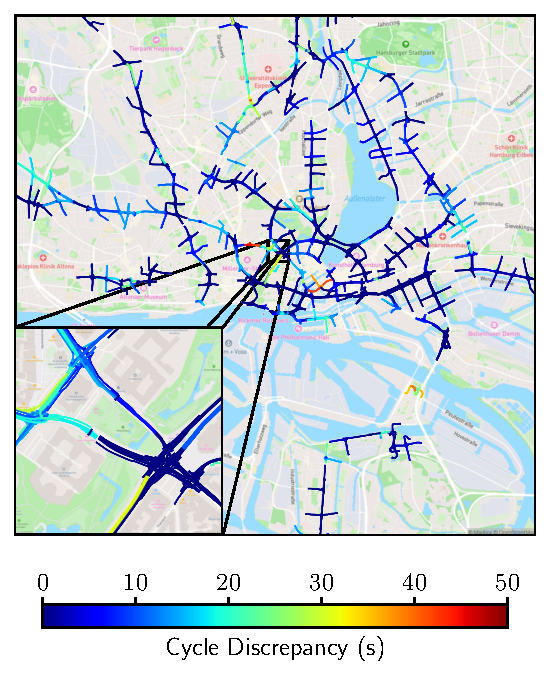
\includegraphics[width=0.46\linewidth]{images/predictability-map.pdf} & 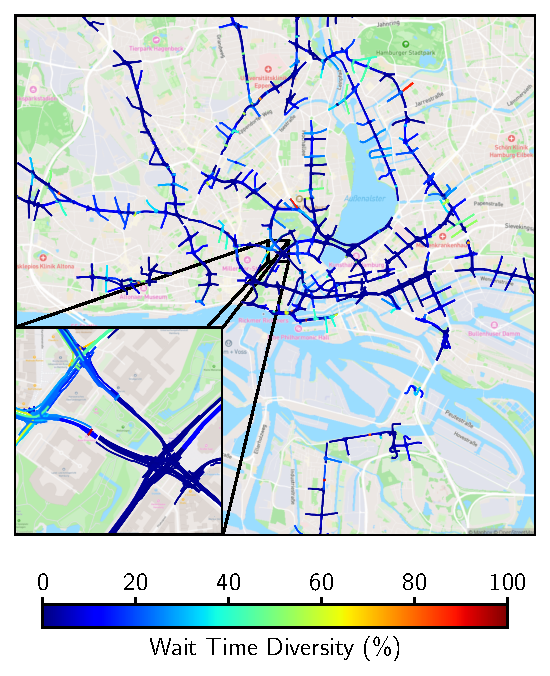
\includegraphics[width=0.46\linewidth]{images/predictability-map-diversity.pdf}
\end{tabular}
\caption{Measured spatial distribution of predictability. Depicted are the traffic light's lanes, colored by their median cycle discrepancy and wait time diversity. Blue parts in the diagram indicate high predictability.} \label{fig:predictability-map}
\end{figure}

\Cref{fig:predictability-map} shows how our predictability metrics are spatially distributed across intersections in Hamburg. While most traffic lights in both images are located in the blue range of the color scale, indicating a high level of predictability, there are a few traffic lights where a higher cycle discrepancy or wait time diversity can be observed. 

As expected, traffic lights with higher unpredictability tend to be located together at the same intersection since they share a joint program and depend on each other's ingress directions. This commonality can be seen in the zoomed-in part of the diagram. However, it can also be seen that traffic lights exhibit only one kind of unpredictability in many cases and not both. Traffic lights exhibiting both unpredictabilities are rare.

\begin{figure}[!t]
    \centering
    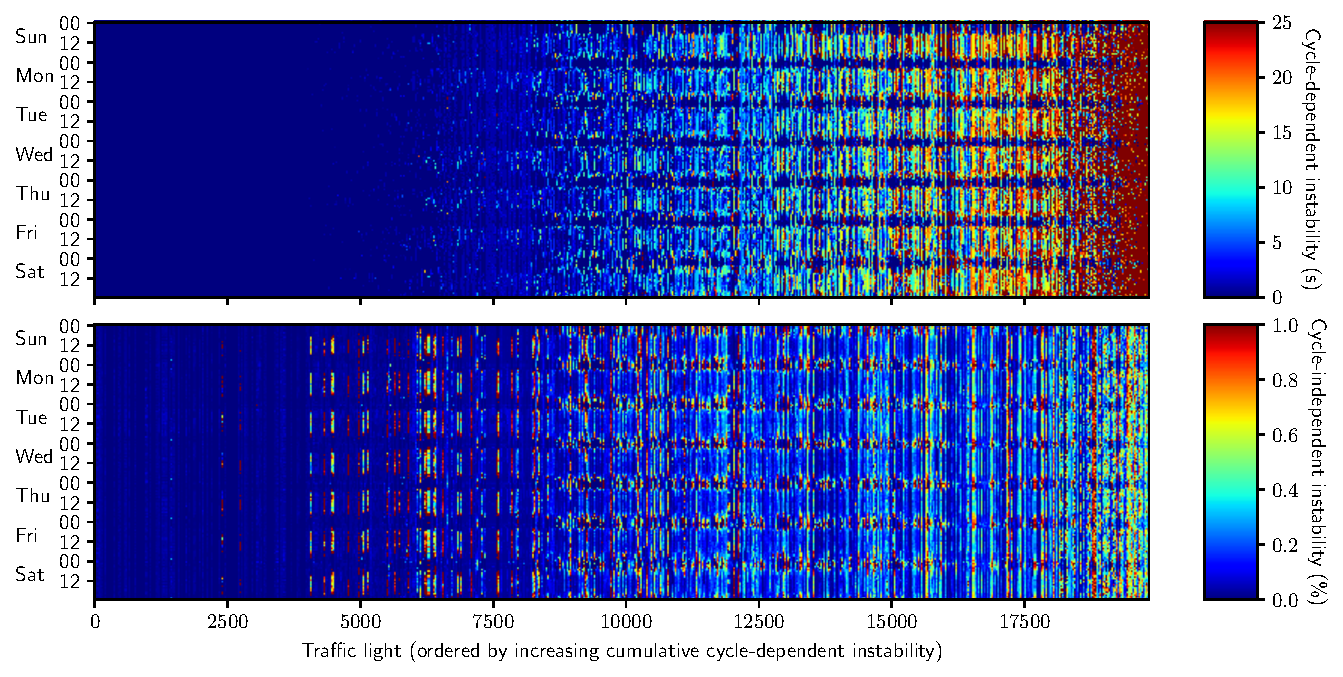
\includegraphics[width=\linewidth]{images/predictability-week-heatmap-per-thing.pdf}
    \caption{Measured weekly progression of both predictability metrics for each traffic light, represented by a vertical line each. Blue parts in the diagram indicate high predictability.}\label{fig:predictability-week-heatmap-per-thing}
\end{figure}

This aspect is explored further in \Cref{fig:predictability-week-heatmap-per-thing}. In the leftmost part of the diagram, traffic lights can be seen that have a low cycle discrepancy but express a high wait time diversity. In the rightmost part, we also find traffic lights with high cycle discrepancy that express low wait time diversity. For these traffic lights, our chosen prediction method may not be ideal. 

Of the evaluated 2,793,786 traffic light hours, 43\% (1,206,817) have a cycle discrepancy of less than 5 seconds and a wait time diversity of less than 10\%. For 67\% of traffic light hours, a cycle discrepancy lower than 5 seconds could be measured, which may also contain higher wait time diversities. Regarding wait time diversity, 77\% of recorded traffic light hours reside below 20\%. Hardly predictable traffic light hours, meaning that the wait time diversity is above 20\% and the cycle discrepancy is above 5 seconds, only comprise 12\% of the overall dataset. Note that the 5-second cycle discrepancy and 20\% wait time diversity were chosen here arbitrarily as a decision boundary, which we felt constituted a good predictability for our scenario. The decision boundary may be chosen more loosely or strictly depending on the prediction accuracy requirements. Nonetheless, the tendency is clear that a large proportion of traffic lights fall into a high predictability (blue) region. 

\begin{figure}[t]
    \centering
    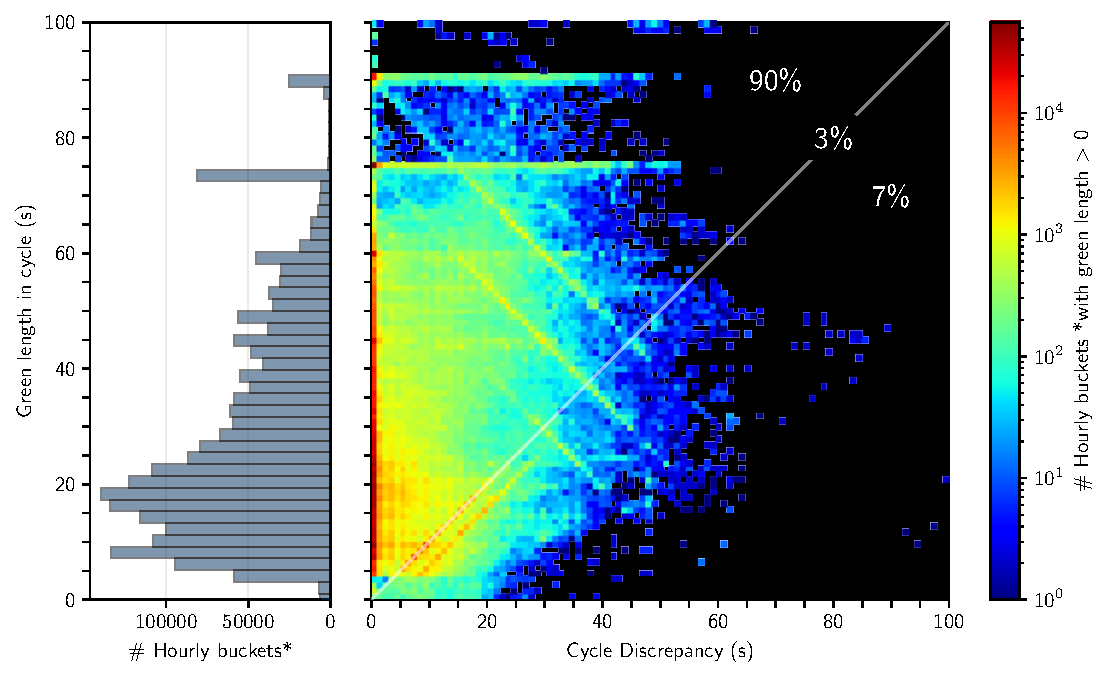
\includegraphics[width=\linewidth]{images/cycle_discrepancy_green_length_heatmap.pdf}
    \caption{Heatmap of the recorded traffic light hours, mapped by their measured green length and cycle discrepancy. Above the depicted diagonal, the cycle discrepancy is shorter than the green length, indicating an overlap of green between cycles and a stable, predictable green phase.}\label{fig:green-length-cycle-discrepancy}
\end{figure}

The results must be viewed in correspondence to the measured green length, which determines how much green overlaps between cycles. Even in the presence of a high cycle discrepancy, a high green overlap would mean that our probabilistic prediction method still finds certain green regions suitable for speed advisory. As seen in \Cref{fig:green-length-cycle-discrepancy} for 90\% of recorded traffic light hours, the median green phase is longer than the median cycle discrepancy. What should be noted here, again, is that most of the traffic light hours reside to the left at a cycle discrepancy of zero seconds. The heatmap colors are scaled logarithmically to reveal more interesting patterns.

Looking more at the revealed patterns may allow us to understand some specific constraints in traffic light behavior. First, a cutoff at 5 seconds of green length can be seen. This follows a best practice of German traffic light planning \cite{TN_libero_mab2}. When extracting and analyzing random examples from specific regions, we find that the horizontal concentrations at 90 seconds, 75 seconds, and 60 seconds primarily stem from traffic lights that switch green for the complete cycle. These buckets are occasionally shifted to the right by red phases of different lengths that interrupt the otherwise switched green phase. Top-left to bottom-right diagonal lines come from traffic lights that extend their green phase until a maximum green duration is reached. Since shorter green phases can be placed more flexibly in the cycle, a decreased green length leads to a higher cycle discrepancy. These constraints could be detected and used to improve the prediction.

\begin{figure}[!t]
    \centering
    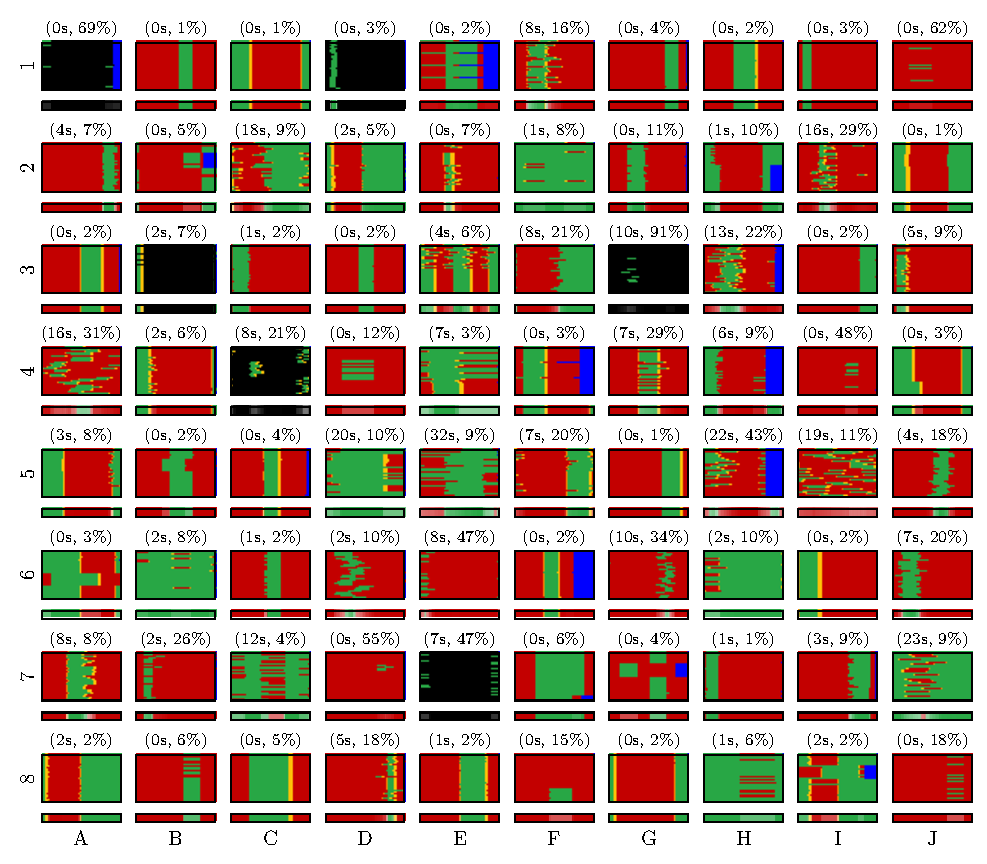
\includegraphics[width=\linewidth]{images/predictability-case-studies.pdf}
    \caption{Random examples of recorded traffic light histories from our database, ordered by their classification according to our two metrics. Below each cycle diagram, a probabilistic prediction based on the cycles is shown. Title format: median (cycle discrepancy, wait time diversity). Low values indicate high predictability. Blue parts of the diagram show cycles that were shorter than the longest recorded cycle during the displayed hour.}\label{fig:types-of-instability}
\end{figure}

To conclude this study, we validate our findings through a random sample of traffic light hours extracted from the recorded database. The extracted sample is highlighted in \Cref{fig:types-of-instability} with the associated values for cycle discrepancy and wait time diversity. Predictions incorporating all cycles in the recorded bucket are also shown to demonstrate how a probabilistic prediction displayed to the user would look. As seen in the visualization, the sample also contains traffic lights that switch between green and black and samples in which the cycle length changed in between, indicated by the blue background.

Overall, most recorded buckets in this sample contain behavior that can be considered predictable. Just looking at the first row, there are already 6 out of 10 cases (B1, C1, E1, G1, H1, I1) with clear columns in the switching pattern that can be easily predicted. There are also cases such as D1, A2, D2, or G2, in which an adaption is visible but limited to a few seconds. In examples such as F2, D5, or H8, we can see traffic lights that are always green until disrupted by a red phase. For cases such as C2, E3, H3, A7, or J7, the traffic adaptivity is more pronounced, as reflected by the high cycle discrepancy score. However, in these cases, as seen before, a joint part in which all cycles are green can still be identified. Examples such as D6 or G6 are more strongly distorted by adaptivity, while these examples also indicate that the green phase centers around a midpoint, as shown in the prediction. An entirely unpredictable pattern is given in I5. As a result, the prediction is fully blurred out. Additionally, with G7, we find one example in which the program seems to have been switched out, indicated by the sudden change in the otherwise stable pattern. Finally, we also see switching behaviors such as E6, J1, J8, or D7, in which the traffic light is switched red most of the time, leading to a red prediction.

While there are examples of apparent adaptive behavior, most recorded switching behaviors contain predictable patterns. This tendency can also be seen in the probabilistic prediction below each cycle diagram, which is only blurred marginally for most predictions. Most predictions contain at least a small fraction of each green phase that is certain. Thus, while highlighting a few interesting examples, our case study generally confirms our previous findings that adaptivity is often only expressed to a minor extent, if at all.

\begin{Summary}[Summary and Discussion of Results]
Our results clearly show that we cannot assume from centralized traffic light data systems that they deliver stable and consistent data. In our case, long-term collaboration with platform operators and active error searching was necessary to stabilize the data system. Previous studies may have been too optimistic here, especially studies that do not work with a real-world system. The highly federated architecture in such systems may lead to complex failure patterns that must be accounted for in the prediction algorithm. 

Through the developed monitoring system, we could identify and help fix multiple systematic issues in Hamburg’s Traffic Lights Data infrastructure, taking over a vital part of the urgently needed quality assurance process. In particular, we could determine a failure pattern related to the traffic controllers that reoccurred daily, helping the operators to scale the data brokers accordingly. Multiple other issues at various parts of the data platform's pipeline were also found and could ultimately be identified and fixed. Even in these harsh circumstances, the probabilistic approach seemed to scale well. It showed good accuracy at most intersections, while the prediction availability was often not optimal due to the described data outages.

Then, we looked at the general predictability of traffic lights in a broader perspective. We found that the predictability decreases during the day, together with the traffic surge, but not as much as expected. We measured that traffic lights switch more adaptively and thus are more unpredictable during the daytime. However, traffic adaptation is minimal for most traffic lights, as predictability only decreases to a limited extent, while many traffic lights remain unaffected. 

Thus, compared to the 90.7\% of traffic lights in Hamburg that should be able to adapt to traffic conditions, we find that this adaptation is only expressed to a minor extent, if at all. Most observed switching patterns align with the cycle length, meaning the probabilistic approach, which highly depends on this alignment, is a good choice. If shifts of the phases in cycles are seen, they are usually shorter than the green time, meaning that some parts of the green phases overlap. This should allow our method to predict green parts of the traffic light switching behavior in most situations with certainty. We confirmed this finding through a randomized case study. Nonetheless, a few intersections were seen at which future experimentation with other methods may be beneficial.
\end{Summary}

\section{Conclusions}

Traffic light prediction provides many opportunities for future intelligent transport systems to enhance the efficiency and safety of traffic, overcoming issues like dilemma zones when approaching an intersection. In practice, however, traffic light prediction is hindered by two issues: obtaining the traffic light data and accounting for unpredictabilities in the switching. 

Previous works mainly resorted to DSRC or cellular V2X to directly obtain traffic light timing information. These systems can use the residual green/red time provided in SPaT messages, externalizing the prediction to the infrastructure provider and ensuring high interoperability between cities. However, as an alternative, we can also use a centralized data platform, making it widely available to all devices with access to the Internet. This solution seems more attractive from a smartphone application's viewpoint. In Hamburg, such a system is available through the Traffic Lights Data platform.

As the Traffic Lights Data platform does not provide traffic light predictions, we needed to interweave an external prediction algorithm based on the available real-time data. To achieve this, we looked for prediction algorithms that are accurate, scalable, and resilient to data outages. A probabilistic approach was identified and integrated based on the available data. To cope with data issues, we implemented a simple error detection that discards erroneous data and degrades the prediction availability in favor of generating fewer false predictions. 

Based on the calculated prediction quality, the developed prediction system works well at most intersections and fulfills our desired capabilities. Only the availability is an issue induced by the frequent data problems. Through a developed monitoring infrastructure, we could help Hamburg's data broker system operators identify reoccurring failures and plan appropriate fixes. From this process, one fundamental conclusion is that employing a centralized traffic light data system may require extensive and continued efforts for data quality assurance. Our monitoring tool was an elemental solution, without which fewer issues would likely have been detected and fixed.

The finding that our prediction algorithm works well stands in contrast to previous works that have repeatedly emphasized the problem of traffic adaptivity. Especially in Hamburg, for which a proportion of 95\% adaptive traffic lights was reported \cite{bodenheimer_enabling_2014} and 90.7\% found based on our research, we expected more significant problems with adverse impacts of traffic adaptivity on our prediction accuracy. Thus, we found a discrepancy between the reported numbers of adaptivity-capable traffic lights and their predictability. 

To investigate this discrepancy further, we spanned a measurement of two unpredictability metrics across Hamburg for four weeks: wait time diversity and cycle discrepancy. The measurements support our finding that only a few traffic lights express adaptivity to a problematic extent for accurate prediction. Most traffic lights express minor shifts, and green phases are often aligned. A few intersections may impose challenges to our chosen prediction algorithm, indicating the need for experimentation with other prediction methods.

Although the established prediction system can be considered a sound foundation for our bike-GLOSA system that circumvented many issues and contributed to the overall understanding of real-world traffic light predictability, there are also open questions for future work. One issue is a lack of ground truth for traffic light messages. Momentarily, we must trust that the traffic light messages contain the correct timing and state information. However, traffic lights sending false timestamps can be a real problem, potentially resulting in a confident prediction that does not reflect the real-world situation. To address this issue, we could think of inferring traffic lights sending invalid data, for example, from user trajectories. 

Even with minor adaptivity, there could still be situations in which the speed advisory is false, requiring users always to pay attention themselves. Calculating probabilities for each second in the prediction is one step in the right direction, ensuring higher trustworthiness and less fluctuation in the speed advisory. However, there are many more steps to go until a prediction can be considered 100\% trustworthy. A more direct collaboration between the prediction system and the internal program switching in traffic lights is needed to attain such a goal, and a history-based prediction may not suffice. In the presence of recent developments in more connected and adaptive traffic control systems, the prediction of traffic lights may become much more challenging in the future.

What remains open is some experimentation with other prediction models on the intersections that have shown low predictability. In our context, we assumed that users could accept a few missing intersections, considering that the prediction turns itself off with highly adaptive traffic lights. That Machine Learning models could be significantly more accurate than a simple probabilistic approach is clear. However, the question is whether these models could also generate a more accurate prediction, considering that poor predictability often arises from erroneous or unavailable data. The resilience of these models against these data issues should be studied further. Latencies in the data and the needed computational resources to predict multiple thousand traffic lights are also key. Future work should focus on this relation to determine under which conditions which model is the most practical.

  \chapter{Traffic Light Matching}\label{ch:matching}

\begin{Summary}[Bibliographical Notes]
This chapter is based on the following two papers in which the author was the principal investigator: 

\cite{matthes2022matching} \fullcite{matthes2022matching}

\cite{matthes2023geo} \fullcite{matthes2023geo}
\end{Summary}

\section{Introduction}

Accurately detecting upcoming traffic lights is crucial for many driving applications. It is not only a safety-critical functionality for (semi)autonomous driving systems but is also essential for bridging the gap between traffic light prediction and speed recommendation. So far, we have considered the traffic light prediction without its relationship to the traffic light's position along the user's trajectory. However, to provide a speed advisory, we must not only know about the predicted timing of the traffic light but also about its position and whether it aligns with the predicted path. A georeferencing is required.

The concept of georeferencing intersections, initially proposed under the name Geometric Intersection Description (GID), was introduced relatively early in the USA in 2008 \cite{cicas-v}. To not only reference the position of traffic lights, but also the specific turns served by them, the turn lane shapes are represented as line geometries crossing the intersection. In this way, it is possible to distinguish between turn directions and find which specific traffic light will be relevant for the vehicle. Today, this information is represented in the internationally standardized MapData (MAP) format that was developed by the SAE\footnote{\url{https://www.sae.org/standards/content/j2735_202309/}} in coevolution with the Signal Phase and Timing (SPaT) message standard.

MAPs, like SPaTs, can reach the road user through various channels, encountering similar transmission issues as SPaTs (see \Cref{ch:prediction}). However, since MAPs are less frequently updated, collecting, transferring to a database, and redistributing the lane geometries is possible. This makes it viable to maintain a centralized directory service in which each lane is mapped. In Hamburg, this centralized directory service is provided by the Traffic Lights Data platform that takes its information from the MAPs developed mainly by engineering bureaus for Hamburg's intersections.

A more significant challenge than the acquisition of intersection topologies is determining which lane on the intersection will be used by a road user approaching it. Typically, there are multiple individual paths that can be chosen when crossing an intersection, and the concrete choice may depend on the user's route, mode of transportation, situation, or general preference. Due to the complexity of real-world traffic, a sudden lane change to align with the traffic perceived as the best option is possible, requiring the system to adapt quickly to the new lane or anticipate the direction in which the user wants to travel. 

While cars are usually restricted by a few available lanes, cyclists or pedestrians often have multiple ambiguous options to cross an intersection. Moreover, cyclists or pedestrians may approach a traffic light from several directions, leading to no clear ingress lane. This leads to the issue that the user's position cannot simply be matched to the nearest ingress lane geometry. Therefore, the problem of matching the correct traffic lights is highly complex, and even more so for cyclist applications.

This chapter aims to address this problem and develop a practical solution for cyclist traffic light matching. First, we review related work and how they address the problem, identifying three core approaches: vision-based using cameras or similar sensors for traffic light identification, location-based using global navigation and satellite systems (GNSS) for lane positioning, and route-based using semantic information such as turns for lane selection. We find that route-based approaches are currently the most promising for bicycle applications. 

Based on this finding, two new methods for route-based bike traffic light matching are proposed: an algorithmic method and a Machine Learning (ML) method. We also focus on approaches that did not yield the desired results and the reasons behind them. Finally, we evaluate the accuracy of the developed approach using multiple ground truths to make well-founded statements about the suitability of the method. A critical summary is provided of the state-of-the-art, developed methods and results to indicate directions for future work.

\section{Related Work}

How traffic light matching is implemented highly differs between simulation studies and real-world studies. Simulation environments usually have an inbuilt capability to determine the upcoming traffic light for each vehicle agent. SUMO, the most popular simulation environment among GLOSA studies \cite{krajzewicz_preparing_2012, erdmann_combining_2013, eckhoff_potentials_2013, tal_vehicular-communications-based_2016, nguyen_efficient_2016, olaverri-monreal_implementation_2018, karoui_efficiency_2018, pariota_green_2019, kloeppel_performance_2019, lu_green_2020, halbach_cooperative_2021, bhattacharyya_assessing_2022, grumert_heads-up_2022, wagner_spatmap_2023}, offers a special API for traffic light matching as part of the TraCI\footnote{\url{https://sumo.dlr.de/docs/TraCI.html}} interface. This interface is utilized by Krajzewicz et al. (2011) \cite{krajzewicz_preparing_2012}, Klöppel et al. (2019) \cite{kloeppel_performance_2019}, Halbach et al. (2021) \cite{halbach_cooperative_2021}, Grumert and Pereira (2022) \cite{grumert_heads-up_2022}, Wagner et al. (2023) \cite{wagner_spatmap_2023}, and Schlamp et al. (2023) \cite{schlamp_2023_glosa}, allowing the authors to find upcoming traffic lights through the simulation environment which knows about the relation between the path network and each traffic light. There are also studies assuming that only one traffic light is associated with each ingress direction at the intersection \cite{xia_indirect_2011, li_multi-vehicles_2014, plianos_predictive_2018}.

However, it is clear that a real-world situation requires quite different solutions. In general, the easiest option here is preselecting the traffic lights in advance. This may be possible in test track environments with a predefined vehicle route and only a few intersections \cite{chen_developing_2022} or corridors \cite{fickas_fast_2019}. Yet, since an approach is desired in which users are allowed to travel freely throughout the city, other more intricate methods must be identified. In the following sections, we will discuss three possible solutions: vision-based, location-based, and route-based approaches.

\subsection{Vision-Based Approaches}

Vision-based approaches primarily originate from the field of autonomous driving. The concept involves utilizing sensors such as radar, cameras, LiDAR, and, in some cases, GNSS to perceive the surrounding environment and identify lanes \cite{lee_avm_2017} \cite{sadli_map-matching-based_2022}. Simultaneous Localization and Mapping (SLAM) is a method within this category that focuses on accurately mapping the environment and locating the vehicle within \cite{cheng_review_2022}. While SLAM captures the environment in real-time, there are also ground truths, known as HD-Maps \cite{kang_lane-level_2020}. Examples of such HD maps include TomTom HD Maps\footnote{\url{https://www.tomtom.com/products/hd-map/}}, NVIDIA DRIVE Map\footnote{\url{https://www.nvidia.com/de-de/self-driving-cars/hd-mapping/}}, or HERE HD Map\footnote{\url{https://www.here.com/platform/HD-live-map}}. These maps provide detailed semantic information, including lane positions and key objects such as traffic lights, and are primarily used for trajectory planning in autonomous vehicles \cite{yang_hdnet_2018}. However, the practicality of these approaches for smartphones is limited due to availability, sensor, and computational constraints.

An approach practical for smartphones is presented by Koukoumidis et al. (2011–2012) \cite{koukoumidis_signalguru_2011, koukoumidis_leveraging_2012}. By mounting the smartphone on the windshield, the position and relevance of traffic lights for speed recommendations are detected only using the smartphone's camera and the user's movement direction. Additionally, the color of the traffic light is detected to obtain its state directly without the need for an external data source. In a collaborative approach, information about traffic light phases is gathered as users pass by, and a prediction is estimated from the sparse crowdsourced data. The designed camera system achieves a per-camera-frame detection accuracy of 87.6\% to 92.2\%, depending on the deployment location and the number of frames recorded standing at a red light. This accuracy could certainly be improved with the object recognition methods available today. However, the main limitation lies elsewhere. Like other vision-based approaches from the field of autonomous driving, the main limitation of this approach is its reliance on a clear line of sight. A handlebar-mounted or stowed-away smartphone, such as in the case of a bike-GLOSA app, does not provide this line of sight. As a consequence, vision-based approaches are generally interesting for the field of autonomous driving or car applications of GLOSA, but not for bike applications.

\subsection{Location-Based Approaches}

Location-based approaches circumvent the issue of requiring a line-of-sight to the traffic light since they only depend on a GNSS location and intersection topologies. The first study identified to express this idea is a technical report by the US Research and Innovative Technology Administration in 2008 \cite{cicas-v}. This report describes a location-based traffic light matching system as part of a Cooperative Intersection Collision Avoidance System (CICAS-V). The described method is relatively simple: as a vehicle approaches the intersection topology, it determines which lane geometries are closest to its position and angle. The closest lane is determined to be relevant for the traffic light service.

Katsaros et al. (2011) \cite{katsaros_performance_2011} were the first to employ this method for a GLOSA system. In their study, the location of each traffic light is extracted from an obtained topology message and then compared to the vehicle's position and heading. Notably, this study was conducted in a SUMO environment. However, as opposed to most other simulation studies, the authors acknowledged that a realistic traffic light matching method was required to employ the GLOSA system in the real world. Nonetheless, not much detail on the methodology and the accuracy of such an approach is presented.

Bernais et al. (2016) \cite{bernais_design_2016} describe a similar approach in a real-world GLOSA system for Braunschweig, Düsseldorf, and Kassel. Instead of matching an individual lane, their approach includes matching upcoming traffic lights based on their stop line. This reduces the complexity of the matching problem significantly since the vehicle's heading can be roughly compared to each ingress direction on the upcoming intersection instead of comparing the position to each individual lane. On the other hand, the stop-line method introduces the need for a multi-lane presentation of the speed advisory since no decision on a specific traffic light is made. This approach is also used by Yunex's traffic light service "APHA" according to the technical documentation \cite{yunex_traffic_v2x-kommunikation_2023}. Other studies, such as by Khan et al. (2021) \cite{khan_eco-drive_2021}, or also the TrafficPilot app, presumably use a similar approach due to the designed user interface. Yet, it is not entirely clear if this assumption is true due to the lack of methodological details and reported results. Thus, it is difficult to reproduce or judge the accuracy of this approach.

Wilson et al. (2017) \cite{wilson_driver_2017}, developing BMW's EnLighten system, studied how a smartphone's inbuilt GNSS capabilities could be utilized to determine the upcoming traffic light. Not much is known about the concrete traffic light matching method, again. However, this study contributes to understanding which challenges a location-based approach may impose in real-world deployments. Wilson et al. (2017) \cite{wilson_driver_2017} were the first to report issues with the smartphone's GNSS. Any issues with the smartphone's GNSS are problematic since the location-based approach assumes that the GNSS is accurate enough and always available to determine the vehicle's position on a lane. However, in their study, the GLOSA system would regularly shut itself down due to losing GNSS connectivity. As the authors reported, this problem leads to user frustration and degraded usability, depending on the malfunctioning rate. A key conclusion is that a perfect GNSS availability cannot always be assumed. 

The GNSS accuracy was determined as another core issue by Stahlmann et al. (2018) \cite{stahlmann_exploring_2018} studying the real-world challenges associated with Audi's GLOSA system. Due to inaccurate geolocation, a similar problem was observed, namely that the system would not enable itself correctly on some occasions since the correct lane could not be identified. Methodologically, the author's approach is equal to the approach described in 2008. However, one variation was included. The car's turn indicator state was incorporated to resolve some ambiguities in the lane selection, especially in the presence of multiple parallel lanes. The information about this indicator was fetched from the car's CAN bus. Therefore, this workaround is strongly tied to a car environment.

A similar issue with the location-based approach was identified by Bhattacharyya et al. (2022) \cite{bhattacharyya_assessing_2022}, who also observed lane mismatching due to the limited GNSS accuracy. In contrast, the authors distinguished the matching inaccuracies in one more category: horizontal mismatching and vertical mismatching. While horizontal mismatching refers to the failing detection of the correct traffic light lane, vertical mismatching refers to the specific problem that intersection topologies may lack the needed height information to distinguish over- and underpasses. Due to this issue, and since GNSS is less accurate in the vertical direction than in the horizontal direction \cite{khomsin_accuracy_2019}, there may be cases where lanes on overpasses or underpasses are not detected correctly.

Bhattacharyya et al. (2022) \cite{bhattacharyya_assessing_2022} propose addressing horizontal mismatching with improved GNSS accuracy. However, which specific methods could be utilized and are practical for a smartphone app is not discussed. State-of-the-art methods for GNSS error correction and dead reckoning usually require the execution of advanced models \cite{werner_machine_2020} associated with draining the smartphone's battery quicker\footnote{In relation to the patent \cite{werner_machine_2020} the Apple Developer Documentation states for the highest available location accuracy: "Because of the extra power requirements, use this level of accuracy only while the device is plugged in." Source: \url{https://developer.apple.com/documentation/corelocation/kcllocationaccuracybestfornavigation}}. Therefore, this method may be more applicable to matching in cars where a power source or wheel odometry for advanced GNSS error correction is available \cite{merriaux_wheel_2014}. Some studies also utilize filters based on lane geometries from HD maps to error-correct the GNSS position \cite{toledo-moreo_lane-level_2010, li_lane-level_2017}. However, this method is not adoptable without the necessary HD map material. Finally, Vedder et al. (2018) \cite{vedder_accurate_2018} show that external antenna boards may also be utilized to improve the GNSS accuracy in bike applications. For a system intended to work without external devices, this is not an option. Thus, it is unlikely that a lane-level accuracy of GNSS in smartphones without large tradeoffs is feasible \cite{lindsey_feasibility_2013}.

Besides GNSS inaccuracies, Stahlmann et al. (2018) \cite{stahlmann_exploring_2018} also pointed out one other factor that is crucial for the location-based approach to work well: long enough lane geometries on the intersection topology. In their work, this parameter is described under the term link length being between 590 to 910 meters, allowing the system to determine a suitable lane early on. The link is drawn centrally on the ingress car lanes toward the corresponding traffic light, thus relying on the fact that cars typically approach an intersection in one direction. This represents a significant limitation for applying this approach to cyclist traffic lights, which are typically associated with multiple ingress directions, for example, via two ingress footpaths shared between cyclists and pedestrians. 

The same applies to the possible turning directions at each intersection. Thus, even if a fully accurate and georeferenced network graph for bike paths can be obtained, the decision about which intersection traversal is chosen still cannot be fully predicted. Although trajectories can be predicted to some extent \cite{rudenko_human_2020}, one key limitation of this method is that it does not capture the planned turns that the user will make. Hence, the extent to which spontaneous or planned lane switches can be predicted in advance is highly limited with this method, reducing the potential activation distance and possibly resulting in speed advisories for the wrong traffic light.

Due to the issues of GNSS inaccuracies and a lack of knowledge of which turn the user will make, location-based approaches are likely not a good option for cyclists. Both problems can only be addressed to a limited extent with GNSS error correction and trajectory prediction. Another challenge may be the shortness of bike lanes, likely leading to an erroneous or delayed matching. With rough matching approaches based on stop lines at intersections, the problem arises that multiple lanes must be visualized through the user interface, trading off with potential additional cognitive load and possible distraction. Furthermore, in case multiple parallel lanes are displayed, the chances are higher that motorists make use of the speed advisory which is intended solely for cyclists, as a measure to motivate cycling. In general, many studies lack the methodological specificity required to fully understand and reproduce the proposed location-based lane-matching approach. Apart from reported challenges associated with a location-based matching approach, there are no reports about the measured per-traffic-light accuracy. 

\subsection{Route-Based Approaches}

Mahler et al. (2012) \cite{mahler_reducing_2012} approach the traffic light matching problem differently from most other GLOSA studies: instead of matching upcoming traffic lights only upon approaching the intersection, they propose doing so in advance through a predefined route that serves as a proxy for the notoriously inaccurate GNSS.

As Mahler et al. (2012) \cite{mahler_reducing_2012} suggested, this route could be automatically determined based on past routes. Alongside this option, there is also the possibility of allowing users to choose their route manually. The route then serves as a predicted path, offering semantic information about upcoming turns. This predicted sequence of turns allows the system to identify suitable traffic lights in advance. However, a critical question arises regarding the map foundation on which the route is calculated and how information about the position of each traffic light is integrated into the route. Mahler et al. (2012) \cite{mahler_reducing_2012} assume that this can be achieved using a public routing API such as Google Maps, where the positions of traffic lights can be easily matched with the route. This conclusion, however, remains somewhat speculative, as the authors do not provide an implementation or results of this proposed method. The method is presented solely as a hypothetical option.

A potential weakness of a route-based approach lies in its dependence on an accurate route that precisely follows the respective lanes. Otherwise, incorrect traffic lights may be selected. This problem can be addressed in two ways: First, we can obtain or generate a routing foundation that allows accurate lane-level routing. This solution will be explored in  \Cref{ch:routing}. Secondly, we can use reasoning to choose the appropriate traffic light instead of simply selecting the closest one, as Mahler et al. (2012) \cite{mahler_reducing_2012} suggested. However, the question is how to implement this spatial reasoning such that an algorithm can fully automatically detect traffic lights along a given route. Since this original idea has not been revisited by other studies, there is a significant knowledge gap in this area.

\begin{Summary}[Summary of Research Gap]
In summary, to provide a speed advisory, it is not only mandatory to have a traffic light's prediction but also to identify which traffic light the user currently travels towards. To solve this problem, vision-based detection is not an option, mainly due to the smartphone's carrying or mounting spots. Alternatively, one could utilize the user's location and current heading to look up nearby traffic lights that align with the user's direction. This approach was identified as the predominant strategy in related work. However, as discussed, GNSS inaccuracies and accurately predicting the upcoming traffic light remain core challenges of the approach. Location-based approaches are likely more suited for multi-lane speed advisory in which a coarse-grained matching suffices. The problem is that multi-lane speed advisory may also come with an increased cognitive load, potentially leading to distraction, and allows motorists to use the speed advisory intended exclusively to motivate cycling. Thus, it is desirable to develop a single-lane traffic light matching method that prefers bike traffic lights. There is a clear research gap in the development of a route-based matching method, which is an underinvestigated but promising approach for a bicycle application of GLOSA. The aim of the following concept is to address this knowledge gap and develop such a method.
\end{Summary}

\section{Concept}

Route-based matching is similar to location-based matching as it assumes the route geometry as an accurate proxy for the user's trajectory. The route's turns can be utilized to infer which specific order of traffic lights will be taken at an intersection. In this way, not only proximal but all traffic lights along the route can be matched in advance. This provides the foundation for displaying the speed advisory early enough such that the cyclist can profit from it. 

In this concept, we will investigate methods that accurately match a few from thousands of traffic lights along a route geometry. The methods are intended to display only one traffic light at a time, preferring bike traffic lights whenever possible, to simplify communicating the speed advisory to the user and avoid abuse by motorists as much as possible. Of course, the methods must also be computationally efficient to allow quick re-matching of the traffic lights in case of a deviation from the intended route.

\begin{figure}[htbp]
\centering
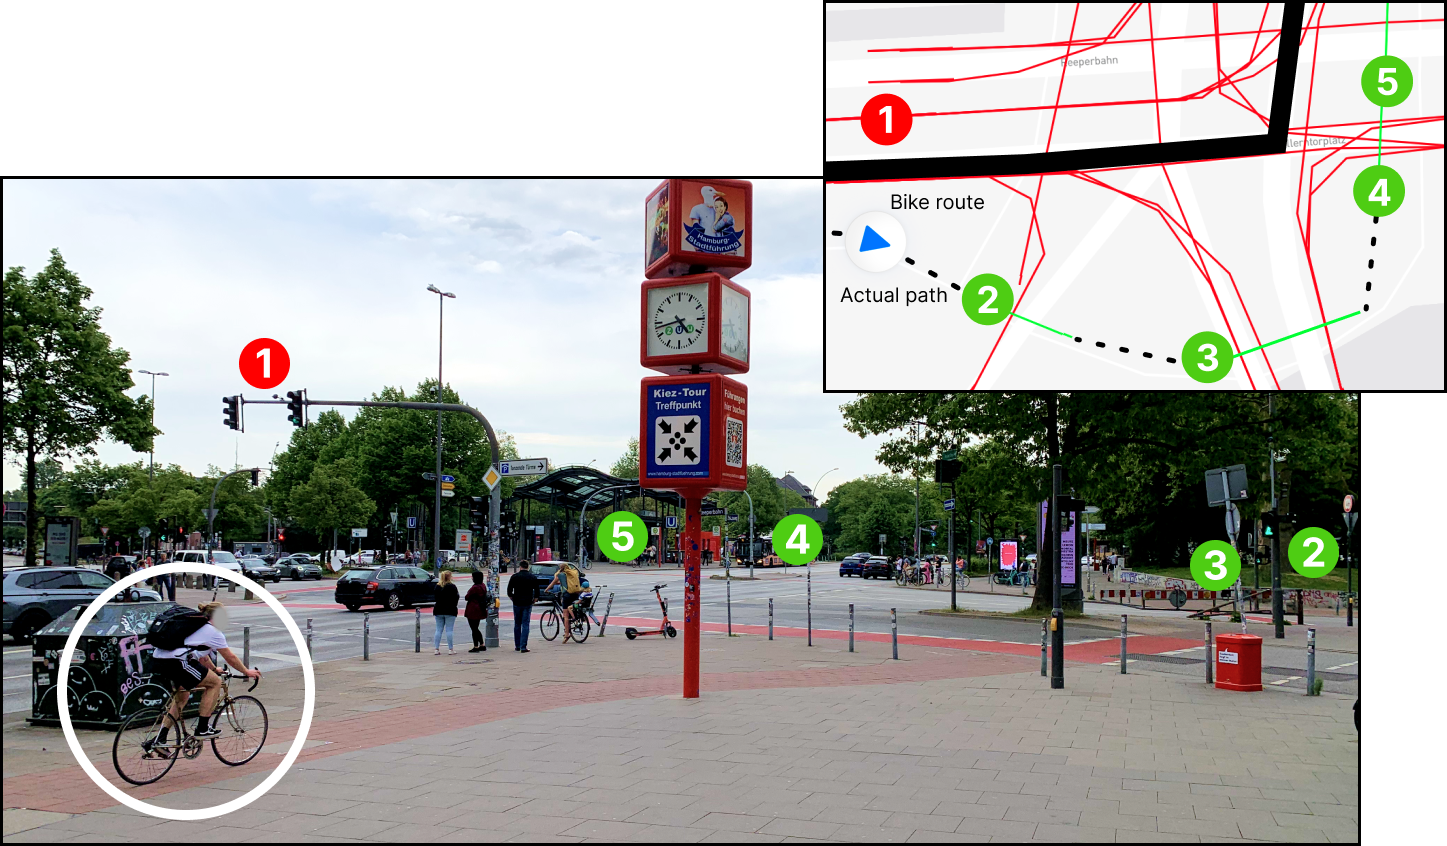
\includegraphics[width=\linewidth]{images/sg-selection-example.png}
\caption{In this case, the OpenStreetMap route does not accurately depict the cyclist's most optimal path and runs over car traffic light 1. In reality, the bike path and four bike/pedestrian traffic lights to the right of the route are utilized: 2, 3, 4, and 5.}
\label{fig:sg-selection-example}
\end{figure}

As a data foundation for the proposed method, intersection (MAP) topologies are utilized that are provided through the Traffic Lights Data platform. For each signal, a line geometry is given that shapes the lane associated with the signal. Which type of traffic is served by the traffic light is also given through the metadata.

Since no precise network graph is available for Hamburg that incorporates both bike paths and traffic light geometries, a different solution must be established to bring together route and traffic light information. In this concept, we will focus on route calculation with publicly available routing foundations such as OpenStreetMap (OSM) and matching the traffic lights along these routes. This solution should then readily apply to other cities as well and has the advantage that we can make use of the bike path metadata provided through the map foundation later on.

However, one challenge we need to solve is that the route geometry and the intersection topologies do not align perfectly. Often, as shown in \Cref{fig:sg-selection-example}, the OSM bike route utilizes car lanes, although bike lanes are available, and generally lacks the level of intersection detail that would be required for a direct lookup. Ideally, the matching method should counteract this problem and reasonably decide between the available traffic lights at an intersection in relation to the route geometry. The goal is to replicate a human's intuition by looking at the route's trajectory over the intersection and selecting the correct bike traffic lights using spatial reasoning.

\subsection{Ground Truth and Benchmark}

It is first important to thoroughly understand what a "correct" traffic light means. The correct traffic lights may not always be clear due to the variety of possible intersection traversals depending on contextual circumstances, personal preference, or even spontaneity. Rather, it is about making the most likely selection and then binding the user to this selection through the user interface.

Assuming that cyclists will follow certain movement patterns at each intersection, and these movement patterns are sufficiently predictable by looking at the intersection layout, we can craft examples for optimal selections. As a result, we obtain a ground truth with combinations of routes and traffic lights predicted by a human to match each given route. In the second step, this ground truth can be utilized to develop and test models for automated traffic light matching.

\begin{figure}[htbp]
\centering
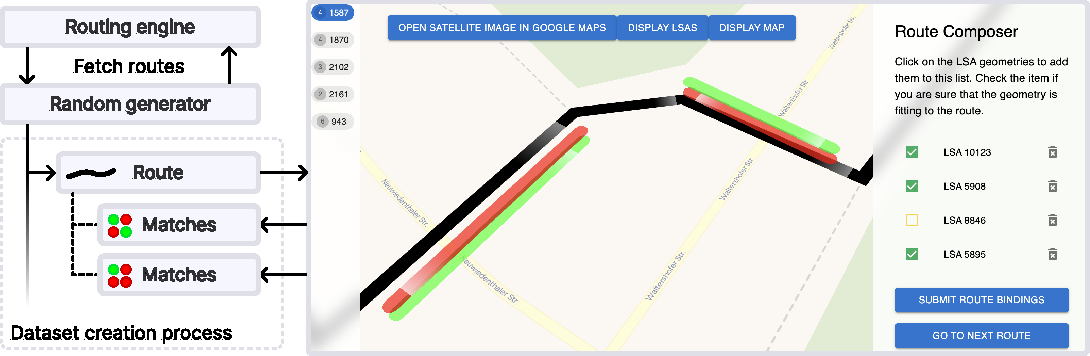
\includegraphics[width=\linewidth]{images/sg-selection-ground-truth.pdf}
\caption{The Route Composer web application.}
\label{fig:sg-selection-ground-truth}
\end{figure}

To create examples for optimal selections of traffic lights, there are multiple options. For example, one could physically ride through Hamburg along arbitrary routes and note down the most likely utilized signals. Ideally, however, the ground truth could be generated in a less time-consuming way without the need to travel to the city of Hamburg or any other remote city in which the application is deployed. 

The proposed tool "Route Composer" delivers this possibility. Instead of physically driving through Hamburg, the Route Composer is a web application that makes it possible to travel virtually along randomly generated routes and label the correct traffic lights. As shown in \Cref{fig:sg-selection-ground-truth}, the Route Composer highlights the traffic lights' and the route's geometries on a map. Then, the traffic lights can be selected by clicking on them in the web application. Once a route is finished, the selected examples are stored for model evaluation.

Independent of the way we generate examples for traffic light matching, they may be biased by limited knowledge of the intersection or personal preference, potentially leading to selections that don't represent the most likely choice. To avoid these improper selections as much as possible, two measures are employed: Assuming that the composing is done carefully enough to notice an ambiguous situation, the Route Composer provides the option to open the current intersection in Google Maps for additional cues. The second measure is a clear ruleset that determines how to handle specific situations:

\begin{enumerate}
\item Consideration is given to traffic flow and the feasibility of safely maneuvering through the intersection.
\item The intersection traversal must be entirely legal according to turn restrictions and street laws.
\item Preference is given to dedicated bicycle lanes or paths indicated by distinct markings or signage.
\item The overall continuity of the route is maintained to ensure a smooth and logical progression.
\item Lanes on the wrong roadside must be avoided.
\item Lanes should never be in an opposing direction to the route.
\end{enumerate}

Based on this ground truth, we can run a benchmark that evaluates the performance of the developed methods. For each route in the ground truth, the matching procedure is executed and produces a list of matched signals. Then, this list of traffic lights is compared to the ground truth, resulting in a number of true negatives, false negatives, true positives, and false positives. Based on these statistics, a benchmark score is calculated.

In the selection of the benchmark metric, a few more considerations are required. Since many of the thousand traffic lights can be excluded entirely by applying a rough distance threshold around the route, a large number of true negatives is expected. These easily excluded traffic lights are not of interest here. What's of interest are the traffic lights near the route for which a more thorough decision is required. Thus, a metric is required that ideally excludes true negatives. The F1 score is chosen here since it only considers true positives (TP), false positives (FP), and false negatives (FN): 

\begin{equation}
\text{F1 Score} = 2 \times \frac{\text{Precision} \times \text{Recall}}{\text{Precision} + \text{Recall}} \quad \text{where} \quad \text{Precision} = \frac{TP}{TP + FP} \quad \text{and} \quad \text{Recall} = \frac{TP}{TP + FN}
\end{equation}

Assuming that especially false-positive or false-negative matches limit the speed advisory's perceived usability, the F1 score is suitable to accurately depict the perceived quality of the matching.

\subsection{Preliminary Approaches}

During the exploration process of potential methods to solve the traffic light matching problem, several methods were tested preliminarily but discarded as they did not perform as well as expected. Before we come to the successful methods for traffic light matching, it is valuable to analyze the failures and learn why these methods did not work as expected. These learnings have been crucial to shape the final solution, as will be presented afterward.

\subsubsection{H3 Approach}

The H3 approach is based on an idea by colleagues who applied a similar method to cluster inaccurately aligned GNSS paths obtaining main directions of intersection traversal and stopping points. The core of this approach is the H3 raster, which subdivides the earth primarily into hexagonal cells\footnote{Strictly speaking, the H3 raster has 12 additional pentagons on every level to complete a seamless shape. See: \url{https://h3geo.org/docs/core-library/restable/}}. On the top resolution level (1), there are 122 cells covering the earth's surface. On level 2, the 122 cells are subdivided into 842 cells, and so forth. As a result, the H3 model contains 15 levels, which are hierarchically connected in a tree structure. Through this hierarchical structure, it is possible to efficiently navigate through the index, e.g., to find neighbor cells. 

In the work by colleagues, after the GNSS samples of each user track were assigned to an H3 cell, the resulting cells each contained a number of samples and travel direction (edge of the H3 cell), resembling a histogram of the trajectories spatially aligned with the intersections. Assuming a normally distributed GNSS scattering around the actual position, the buckets could then be used to statistically sift out the most frequently used pathways of cyclists. Minor GNSS errors or individualities in the user movement don't fall into weight as they are clustered together. Since this approach was described as remarkably successful, the fundamental idea was further explored to identify potential methods for aligning the traffic light geometries with the inaccurate bike route.

\begin{figure}[htbp]
\centering
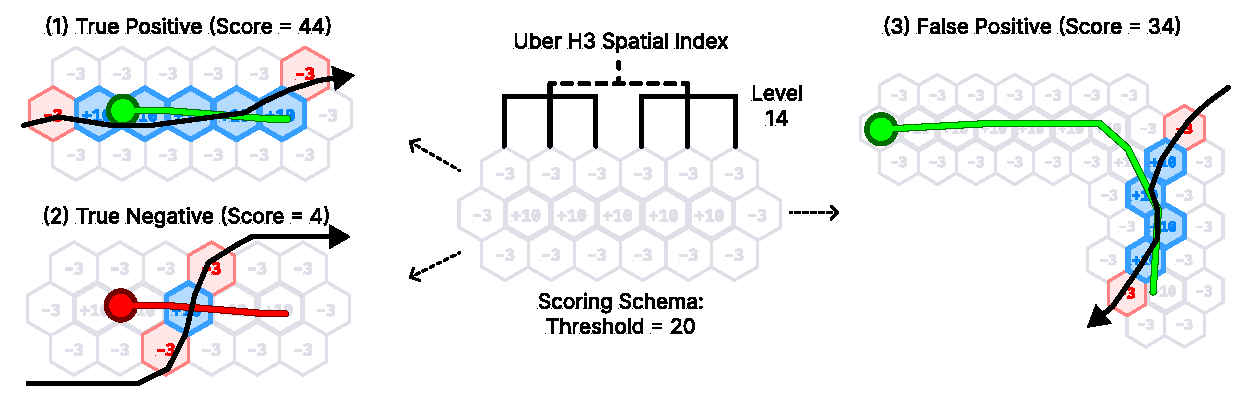
\includegraphics[width=\linewidth]{images/sg-selection-h3-approach.pdf}
\caption{Illustration of the matching procedure behind the developed H3 approach.}
\label{fig:sg-selection-h3-approach}
\end{figure}

The initial idea was to count the cells aligned between route geometry and traffic light geometries. If sufficient overlap is found, the traffic light is detected as a match. After testing multiple H3 levels, the H3 level 14 was determined empirically to provide the best tradeoff between resolution and tolerance to imperfect alignment. To emphasize the importance of a near-parallel alignment, a ring-based scoring schema as illustrated in \Cref{fig:sg-selection-h3-approach} was tested that penalizes crossing geometries (2) and favors parallel-aligned geometries (1). This ring-based scoring schema makes use of H3's tree structure to efficiently find neighboring cells of the traffic light geometry.

Nonetheless, a very significant challenge is to find a suitable scoring threshold for the number of matched cells until a traffic light is counted as a "match." Some traffic light geometries may be only a few meters long, while others are much longer. Since longer geometries contain more cells, it is more likely that longer geometries are false-positively matched to the route, while short geometries often produce false negatives. After testing multiple different scoring schemas and thresholds and coming to the final scoring schema highlighted in \Cref{fig:sg-selection-h3-approach}, it was not possible to achieve a sufficiently good matching. In the developed benchmark, an F1 score of 50\% was never exceeded. 

One identified possibility for improvement was to apply a relative scoring schema for each signal. Instead of applying absolute values to each H3 cell around the line geometry, the scoring schema would be scaled inversely proportional to the number of cells. This means that a longer line geometry would have more cells with lower individual scores compared to a short geometry. Ideally, the result would be a normalized alignment score for each traffic light geometry that can be subjected to a universal threshold. Figuratively, the score would depict how much both geometries align. However, this potential solution was not thoroughly explored due to other systematic limitations of the H3 approach.

\begin{figure}[htbp]
\centering
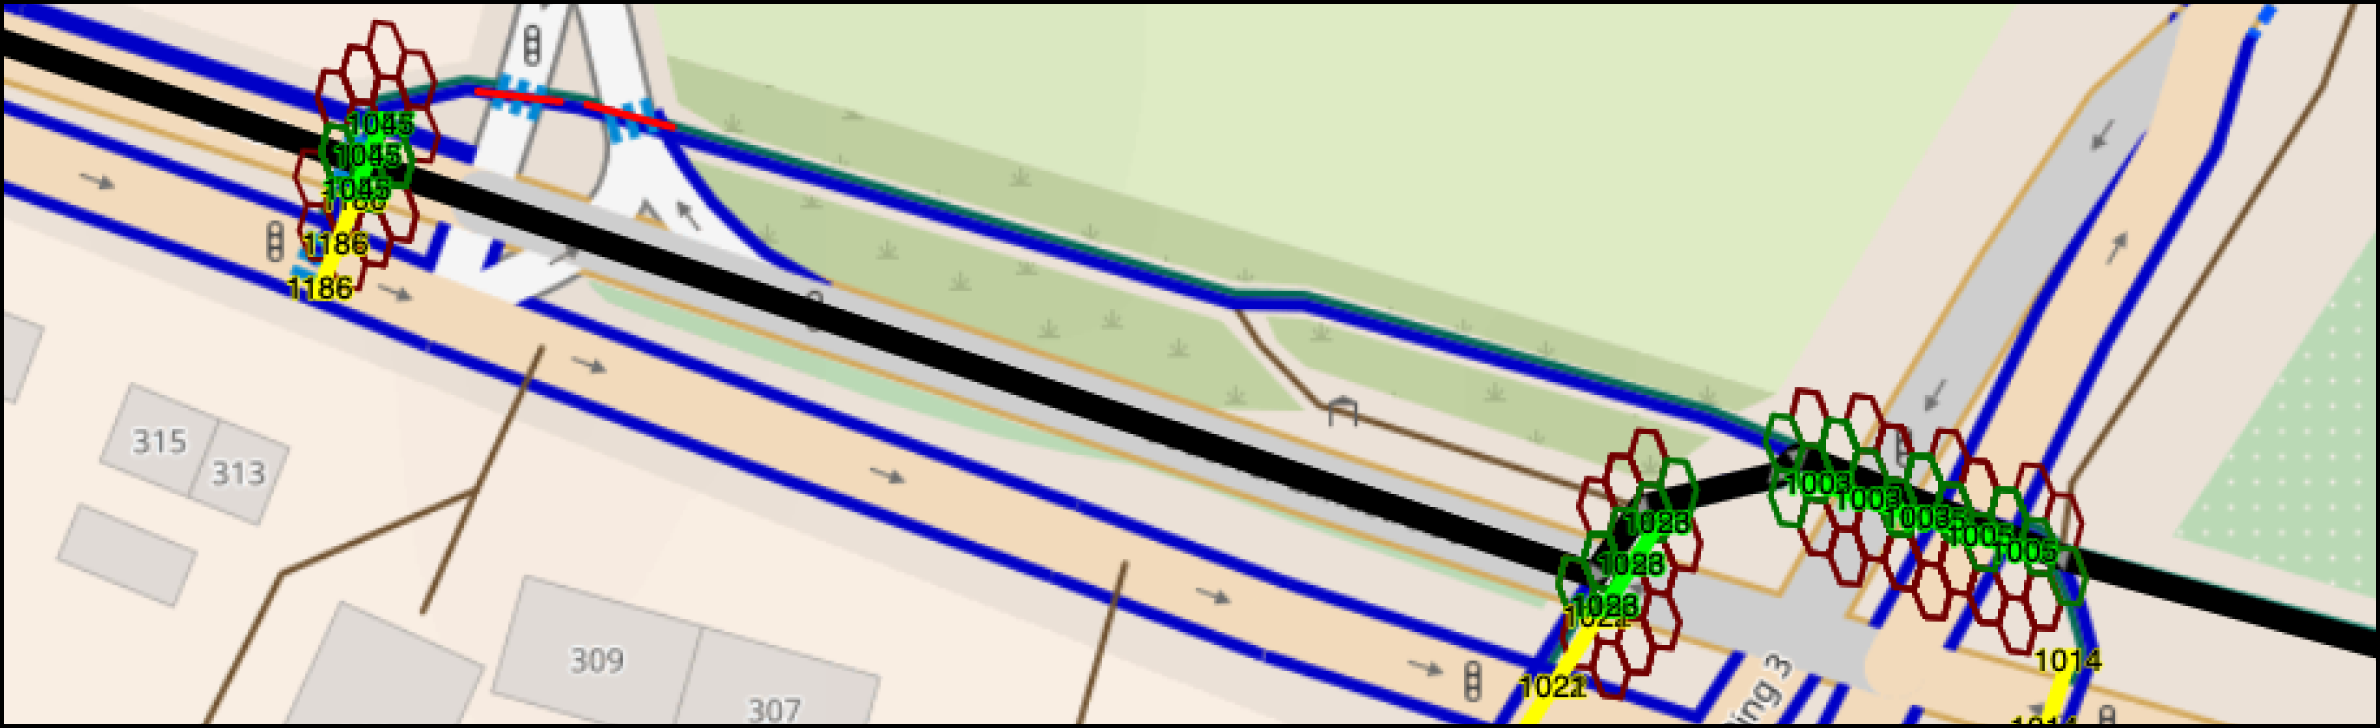
\includegraphics[width=\linewidth]{images/sg-selection-h3-example.png}
\caption{Example of four traffic lights that were matched using the H3 approach along the route.}
\label{fig:sg-selection-h3-example}
\end{figure}

The main limitation of the H3 approach is that it assumes that the route geometry is near enough to the matching traffic light geometries. However, considering OSM's mixed coverage of bike paths, many false negatives were produced when the route was mapped on the car lanes, while the appropriate bike traffic light was located on the bike path a few meters to the side of the road. 

A potential solution to this problem would be to choose a larger raster, but this would worsen the score even more since many signals' geometries are no longer captured adequately. Instead, they would resemble a circular "blob", as highlighted on the left side of \Cref{fig:sg-selection-h3-example}. The "blob" problem does not only appear when upscaling the raster to H3 level 13. It appears at level 14 as well. Some traffic lights would have such short geometries that only one H3 cell was matched, especially concerning pedestrian traffic lights crossing the road. Since many of these traffic lights are aligned orthogonally to the road's direction, the loss of the signal's direction information in the "blob"-shaped scoring schema would ultimately lead to erroneous matchings. Increasing the resolution level to 15 would mitigate this problem and introduce a more shaped raster around the line geometries, but would again increase the volatility against offset traffic lights along the route.

Due to these issues, the H3-based approach for traffic light matching was not further explored. The takeaway from this approach is that close alignment does not sufficiently model matching traffic lights along a route geometry. Instead, sometimes, the traffic light geometries may be offset from the route, especially if the route is snapped onto the car lanes.

\subsubsection{Graph Approach}

The second approach is inspired by the map-matching procedure proposed by Newson and Krumm in 2009 \cite{newson_hidden_2009}. Their proposed method matches GNSS trajectories to the road network by building a transition graph between each GNSS sample and the nearby roads. After the graph is created, each transition is marked with a transition probability. In their approach, the most probable path through the transitions is calculated using the Viterbi algorithm to find the most likely sequence of roads that were taken. This approach can be transferred over to traffic light matching, interpreting the route geometry as GNSS trajectory and the traffic light geometries as road segments.

\begin{figure}[htbp]
\centering
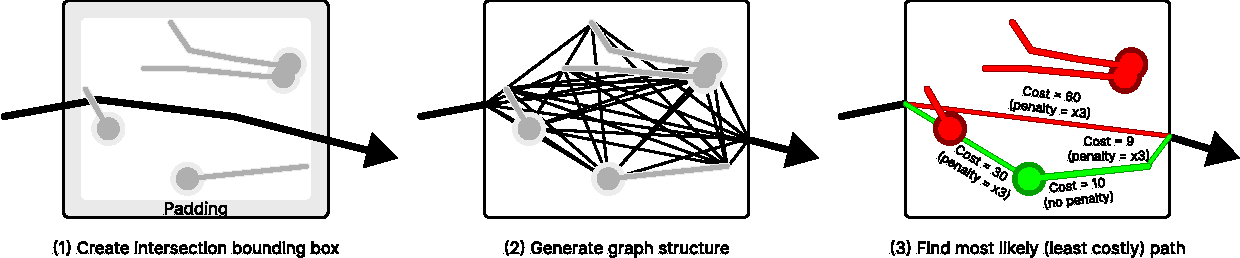
\includegraphics[width=\linewidth]{images/sg-selection-graph-approach.pdf}
\caption{Steps for traffic light matching in the graph-based approach.}
\label{fig:sg-selection-graph-approach}
\end{figure}

The proposed approach operates as illustrated in \Cref{fig:sg-selection-graph-approach}. First, traffic lights along the route are prefiltered using a rough distance threshold of 20m. The remaining traffic lights are clustered into intersections based on the intersection node ID. Around each of these intersections, the procedure undergoes three steps: (1) A bounding box is calculated with an additional padding. The route enters and exits the bounding box at one point. (2) A fully connected graph is generated between the route's entry and exit points and each traffic light geometry's start and end points. (3) A cost is assigned to each transition in the graph based on the transition's length. Finally, the least costly path is calculated using the Dijkstra pathfinding algorithm. The idea is that the least costly path represents the most likely utilized trajectory over the traffic light geometries.

The cost function is defined to penalize traversal between signals, and traversal using the traffic lights is preferred. Otherwise, the most optimal path would always be the direct connection between the entry and exit points. Specifically, every transition in the graph  $(p_{1} \rightarrow p_{2})$ has the cost $dist(p_{1}, p_{2})$, while transitions between traffic lights have the cost $dist(p_{1}, p_{2}) \times \text{penalty}$. Thus, the penalty value represents a hyperparameter of the model together with the dimensions of the intersection padding. 

Which penalty value and intersection padding to choose may depend on each intersection's characteristics. Thus, defining these hyperparameters by hand would not be the best option. A better option is to utilize a tuning algorithm that automatically approximates the optimal configuration based on the developed ground truth. Specifically, the Tree-Structured Parzen Estimator hyperparameter tuning algorithm \cite{ozaki_multiobjective_2020} is utilized. This tuner considers each hyperparameter (intersection padding and penalty) independently from each other. During the tuning, the model undergoes inference for all routes in the dataset (one trial). After each of these trials, the F1 score is evaluated, and the hyperparameters are adjusted by the tuner into a direction the tuner estimates will result in a better score.

\begin{figure}[htbp]
\centering
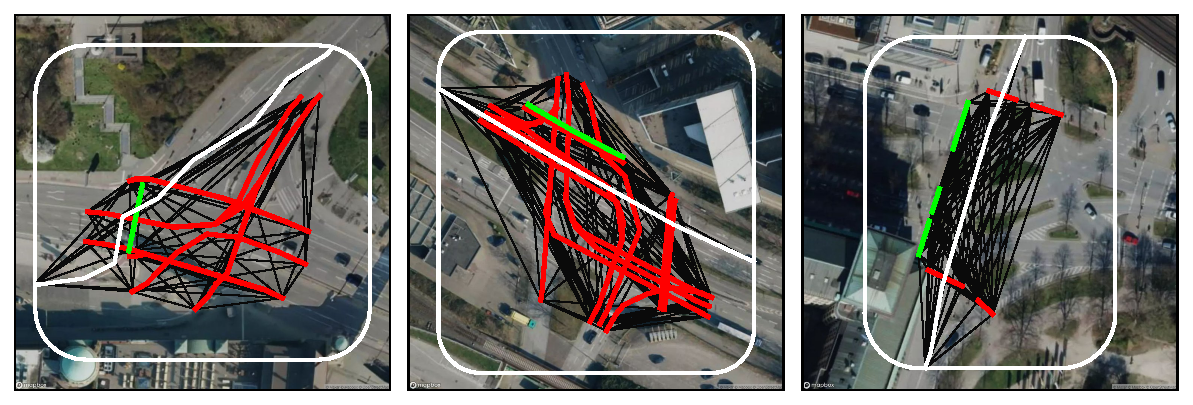
\includegraphics[width=\linewidth]{images/matching-dijkstra-correct.pdf}
\caption{Examples of correct matching using the graph approach.}
\label{fig:sg-selection-graph-example}
\end{figure}

After tuning the model to the ground truth, the model reached an F1 score of 75.4\% (penalty = 2.87, padding = 25m). As a distance function, this version of the model utilizes the Euclidean distance between the coordinates in the WGS84 projection system. Correct matchings from this model highlighted in \Cref{fig:sg-selection-graph-example} indicate the model's capabilities. The model would perform well even in scenarios where the signal's geometry is offset to the route and thus has large advantages over the H3 approach, as reflected in the improved F1 score.

\begin{figure}[htbp]
\centering
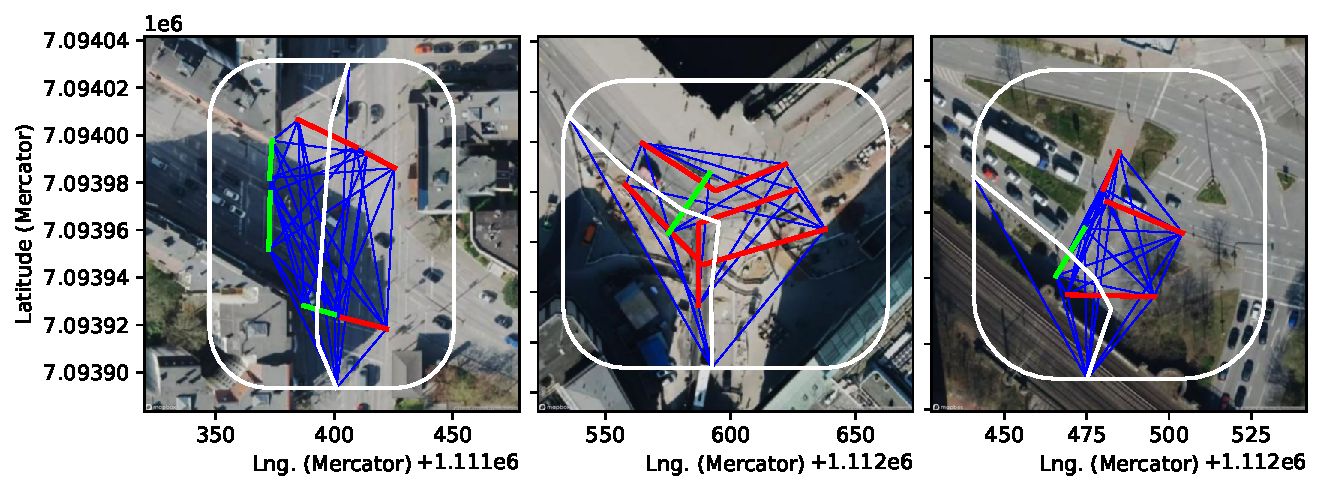
\includegraphics[width=\linewidth]{images/matching-dijkstra-incorrect.pdf}
\caption{Examples of false matching using the graph approach.}
\label{fig:sg-selection-graph-fails}
\end{figure}

However, the final result is still not convincing, considering that the measured score of 75.4\% represents a training F1 score and was not evaluated on unseen data. By studying many error cases, one particular weakness was identified. As highlighted in \Cref{fig:sg-selection-graph-fails}, the model would struggle particularly with right or left turns at intersections. In these cases, the route exits the bounding box on an adjacent edge to the ingress's edge. This means that the direct distance from the ingress point to the egress point is often lower than the path over the correct signals' geometries. As a result, the model tends to shortcut directly to the intersection exit. To cope with these cases, two potential solutions were identified:

\begin{enumerate}
    \item Increasing the penalty for traveling off a signal's geometry. A separate penalty could be applied in cases where the ingress and egress edges of the bounding box are adjacent to avoid shortcuts.
    \item  Modifying the graph generation procedure to strictly "go back" to the nearest point on the route after each traversal of a signal's geometry. Thus, the penalty for attempted shortcuts (going off the route) would increase drastically.
\end{enumerate}

Option one initially may seem like a good choice here. However, this strategy would worsen another problem highlighted in \Cref{fig:sg-selection-graph-fails}: often, traffic light geometries are falsely traversed simply because their exit point is slightly more proximal to the egress point. A higher penalty amplifies this problem. Thus, option two was implemented instead. 

\begin{figure}[htbp]
\centering
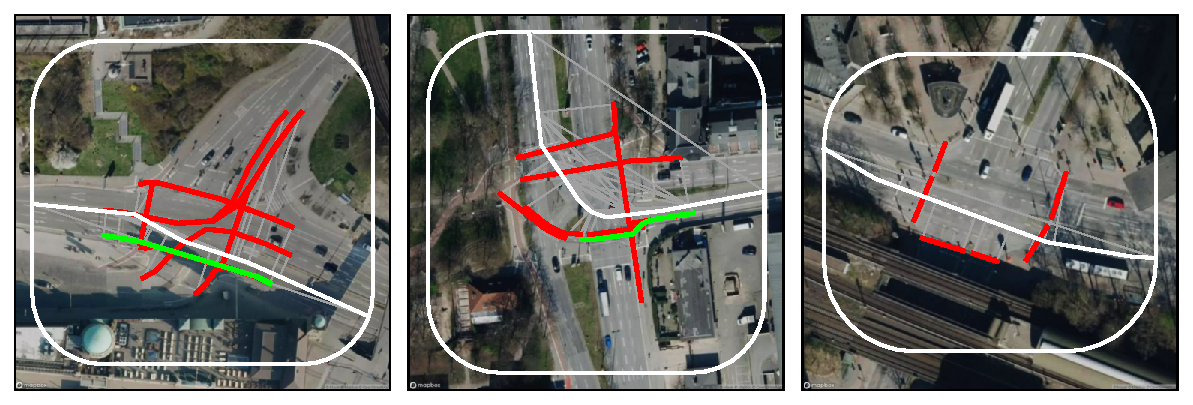
\includegraphics[width=\linewidth]{images/matching-dijkstra-strict.pdf}
\caption{Examples of matching using the adjusted graph generation procedure.}
\label{fig:sg-selection-graph-strict}
\end{figure}

Unfortunately, the result of the adjusted graph generation procedure is a worse F1 score after hyperparameter tuning of 60.7\% (penalty = 9.68, intersection padding = 42m). In many cases, the model would now avoid shortcutting as intended, but the model would also be noticeably more strict. The reason is that the signals' geometries are no longer connected to each other but rather through the route (see \Cref{fig:sg-selection-graph-strict}). Jumping on and off the signals' geometries would often be a worse option for the pathfinding algorithm than staying on the route, even with a remarkably higher penalty. 

Another variation of the graph-based approach would be to cut out the intersections, reconnect the OSM paths via the traffic light geometries, and then calculate the route using these. However, the main problems here would probably be similar, especially the problem of connecting the traffic light geometries with each other and the problem of stitching at the edges. Thus, this idea was not further explored.

Although the developed graph-based methods initially promised good results, they were ultimately not further studied in favor of more promising ideas. Even if the graph approach seems less susceptible to offsets and longer traffic light geometries, it clearly falls short when considering the curvature and not only the absolute location of the traffic light geometries. In the end, only each traffic light geometry's start and end points are considered. However, the curvature is similarly important to decide which traffic light could match the associated route.

\subsubsection{Map-Matching Approach}

A positive learning of the graph-based approach is that the map-matching problem of Newson and Krumm (2009) \cite{newson_hidden_2009} is, in theory, very similar to the problem we are trying to solve. Another idea based on this approach would be to map-match the traffic light geometries onto the OSM road network, fusing both map sources and allowing for a direct traffic light lookup.

\begin{figure}[htbp]
\centering
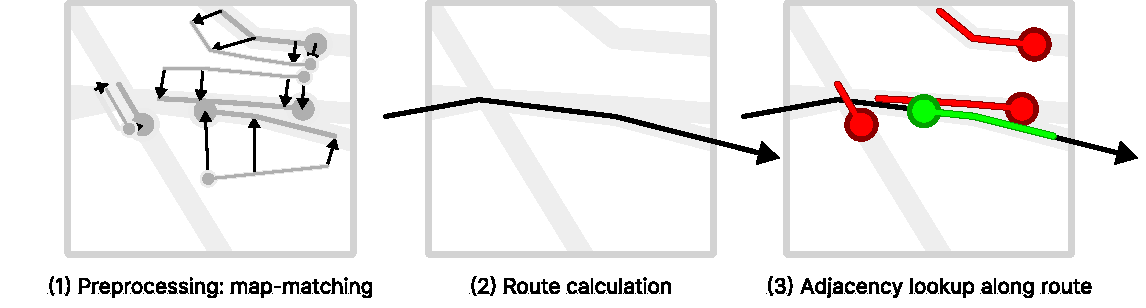
\includegraphics[width=\linewidth]{images/sg-selection-map-matching-approach.pdf}
\caption{Steps for map-matching traffic lights onto the routing foundation.}
\label{fig:sg-selection-map-matching-approach}
\end{figure}

\Cref{fig:sg-selection-map-matching-approach} illustrates the proposed procedure, consisting of three steps: (1) In a preprocessing step, the traffic light geometries are map-matched onto the routing foundation. As a result, the traffic light geometries align with the routing foundation's topology. (2) The route is calculated using the same routing foundation. (3) All traffic lights that perfectly align with the route's geometry are matched.

The approach by Newson and Krumm (2009) \cite{newson_hidden_2009} is utilized as a map-matching procedure. This approach is implemented by default in the GraphHopper routing engine and can be accessed through its map-matching API\footnote{\url{https://docs.graphhopper.com/\#tag/Map-Matching-API}}. Each traffic light geometry is transformed into a compatible format (GPX) and sent to the map-matching API, where it is projected onto the integrated routing foundation.

\begin{figure}[htbp]
\centering
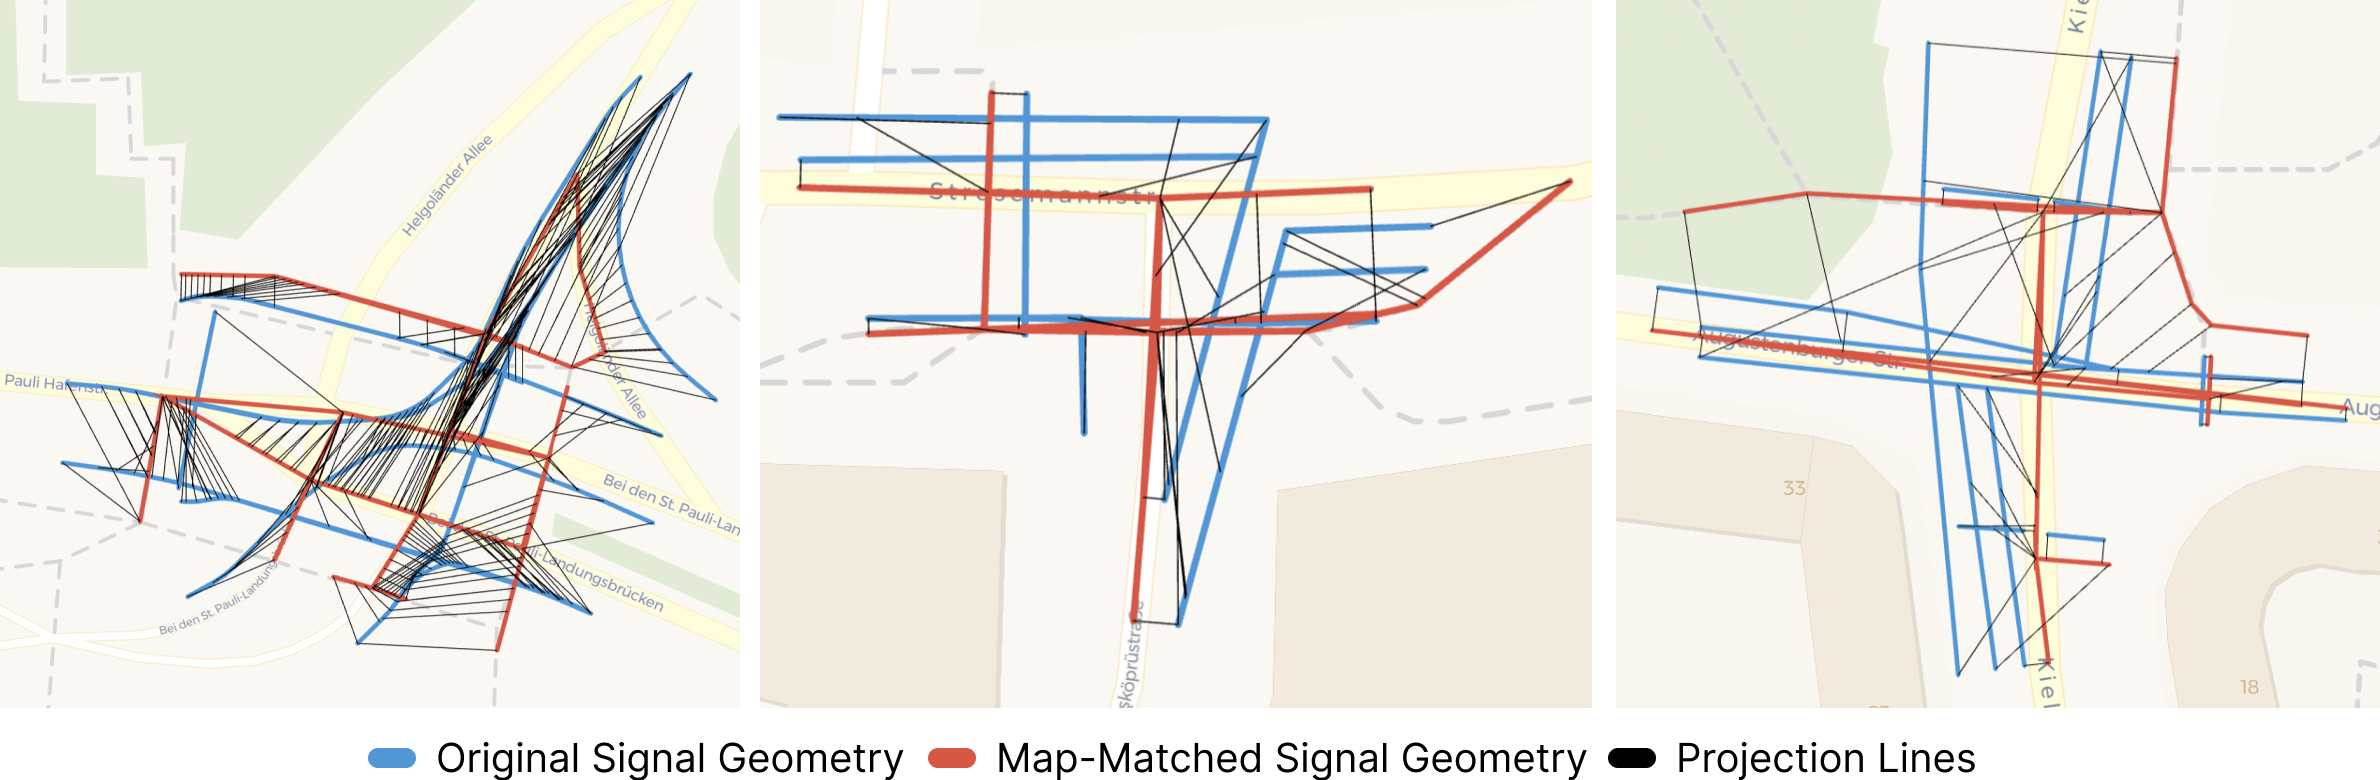
\includegraphics[width=\linewidth]{images/sg-selection-map-matching-fails.png}
\caption{Distortion of traffic light geometries after map-matching.}
\label{fig:sg-selection-map-matching-fails}
\end{figure}

Despite the promising idea, when testing the approach with the OSM routing foundation, a substantial problem was determined. Although it was possible to project the traffic light geometries onto the routing foundation, they were completely distorted during the process. Examples of this distortion are highlighted in \Cref{fig:sg-selection-map-matching-fails}. These distortions may be amplified by the problem that traffic light geometries are usually shorter than typical GNSS trajectories for which the map-matching approach was initially conceived. What's clear is that, without enough intersection detail in the routing foundation, the map-matching procedure would often fail to find a suitable projection. Moreover, multiple traffic lights may be matched onto the same path segment, resulting in an ambiguous matching. 

Since not only bike traffic lights are represented in the system but also traffic lights shared between cars/buses and bikes, this approach would require a routing foundation that represents all of the respective paths (not only bike paths) noticeably more accurately than OSM, such as a multimodal HD map. Whether this approach applies to such a map could not be tested as none was available. Due to these findings, the map-matching method was also not investigated further.

\subsection{Algorithmic Filtering Approach}

The preliminary H3, graph, and map-matching approaches have not been successful but provided a deeper understanding of the problem. First, an ideal matching procedure should be robust against offsets of the traffic light geometries from the route, especially in cases when the route geometry is mapped on the road while the bike traffic light is alongside. Second, the matching procedure must handle long and short traffic light geometries similarly well. 

\begin{figure}[htbp]
\centering
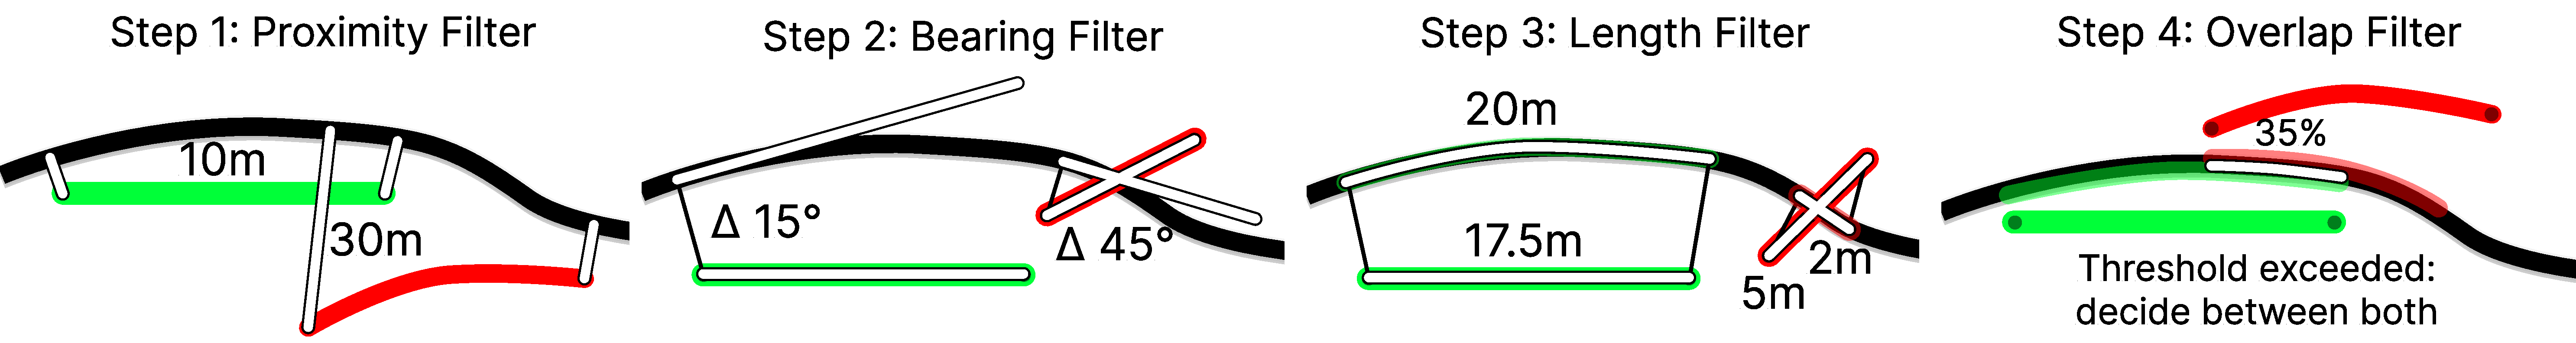
\includegraphics[width=\linewidth]{images/sg-matching-filters.pdf}
\caption{Filtering steps for matching with the algorithmic approach.}
\label{fig:sg-matching-filters}
\end{figure}

Most importantly, it is crucial to consider the absolute location of the traffic light geometries along the route and their geometrical properties in relation to the route. If the signal's geometry is aligned relatively near the route and follows its curvature, it is likely to match the route. The question is how to mathematically model this relation and tell apart edge cases.

One solution is to tell apart matching from non-matching traffic light geometries by a geometrical comparison with the route. In four filtering steps, specific geometric thresholds are applied to filter out traffic lights that are likely no match. The idea is that each step catches a specific type of misalignment with the route, such that, in the end, only the wanted matches remain. As shown in \Cref{fig:sg-matching-filters}, four filtering steps are employed: proximity filter, bearing filter, length filter, and overlap filter.

\paragraph{Step 1 -- Distance Filter:} Step one focuses on coarsely excluding a large proportion of the traffic lights in the city area through a distance threshold $t_{dist}$ from the route. This step is efficiently executed through a PostGIS database using the \texttt{ST\_Distance}\footnote{\url{https://postgis.net/docs/en/ST\_Distance.html}} query.

\paragraph{Step 2 -- Bearing Filter:} As a next step, the bearing between the signal's geometry and the route is compared. Hereby, we can exclude traffic lights that are angled too steeply or even inverted to the route. As a foundation, the atan2 function is used to calculate the bearing between two coordinates on the earth\footnote{\url{https://www.movable-type.co.uk/scripts/latlong.html}}:

\begin{equation}
x(c_1, c_2) = sin(lon_2 - lon_1) \times cos(lat_2)
\end{equation}
\begin{equation}
y(c_1, c_2) = cos(lat_1) \times sin(lat_2) - (sin(lat_1) \times cos(lat_2) \times cos(lon_2 - lon_1))
\end{equation}
\begin{equation}
bear(c_1, c_2) = atan2(x(c_1, c_2), y(c_1, c_2))
\end{equation}

where $c_1 = (lat_1, lng_1)$ and $c_2 = (lat_2, lng_2)$ are WGS84 coordinates (in radians). As a result, we can calculate the bearing of the signal's geometry $(c_1, \dots, c_n)$ based on its first two coordinates. To compare this bearing to the route geometry, the signal's geometry is projected onto the route. Every coordinate $(c_1, \dots, c_n)$ is mapped to the nearest point on the route geometry $(\bar{c_1}, \dots, \bar{c_n})$. Then, the bearing diff $\bar{\Delta}_{bear_1}$ is calculated as:

\begin{equation}
    \bar{\Delta}_{bear_{i=1}} = 
        abs(\underbrace{bear(c_{i=1}, c_{i+1=2})}_{\text{Bearing of traffic light geometry}} - \underbrace{bear(\bar{c}_{i=1}, \bar{c}_{i+1=2})}_{\text{Bearing of projection on route}})
\end{equation}

The bearing diff $\bar{\Delta}_{bear_1}$ denotes how much the signal's angle is different from the route's angle at the nearest point to the first traffic light geometry coordinate. The calculated value can be subjected to a bearing threshold $t_{bear}$ which defines if the signal's geometry is counted as a match or not:

\begin{equation}
\Psi_{bear_{i=1}} = 
    \begin{cases}
            1,& \text{if } \bar{\Delta}_{bear_{i=1}} \in \left(-t_{bear}, t_{bear}\right)\\
            0,              & \text{otherwise}
        \end{cases}
\end{equation}

where $\Psi_{bear_{i=1}} = 1$ means that the segment is angled similarly enough to the nearby route and is therefore a match. All traffic lights that are not a match ($\Psi_{bear_{i=1}} = 0$) are filtered out. For example, if $t_{bear} = 45°$, we will filter out all geometries whose first coordinate is angled more than $\pm 45°$ relative to the projection onto the route. 

\begin{figure}[htbp]
\centering
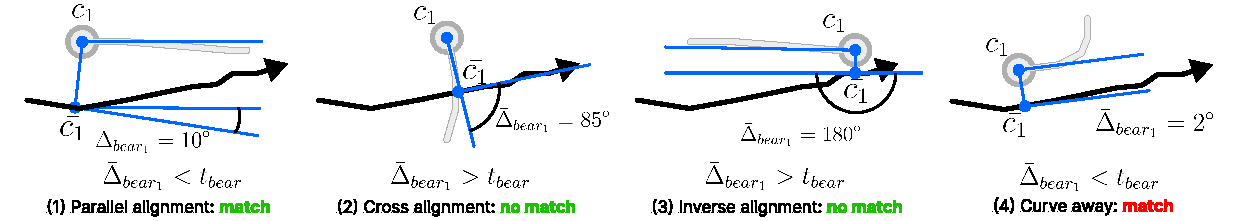
\includegraphics[width=\linewidth]{images/sg-selection-bearing-filter.pdf}
\caption{Examples for bearing matching based on traffic light geometry's first coordinate.}
\label{fig:sg-selection-bearing-filter}
\end{figure}

This process is drawn in \Cref{fig:sg-selection-bearing-filter}. In cases (1), (2), and (3), the alignment of both geometries is classified correctly. However, (4) illustrates one particular weakness: traffic light geometries initially aligned but then curving away from the route are not filtered out correctly. The reason is that only the first coordinate is compared, and not the complete geometry. To compare the complete geometry, all coordinates $c_i$ of the traffic light geometry are compared to the route. Then, a weighted sum $\phi_{bear}$ is calculated, incorporating the length of each geometry segment relative to the complete geometry. In this way, longer parts of the signal's geometry are emphasized:


\begin{equation} 
\phi_{bear} = 
    \underbrace{\sum_{i=1}^{n-1} 
    \frac{\Psi_{bear_i}}{dist(c_i, c_{i+1})}}_{\text{Sum of matching segment lengths}}
    \times
    \underbrace{(\sum_{i=1}^{n-1} dist(c_i, c_{i+1}))^{-1}}_{\text{Sum of segment lengths}}
\end{equation}

where $dist$ is calculated as the Euclidean distance and $n$ is the number of coordinates in the signal's geometry. As a result, $\phi_{bear}$ is normalized between 0 and 1. $\phi_{bear} = 0$ means none of the traffic light geometry's segments matches the angular threshold $t_{bear}$, while a value of 1 represents a full match. To determine the decision boundary between match and no match, $\phi_{bear}$ is subjected to another threshold $t_{bear\_sum} \in [0, 1]$. This threshold is chosen such that traffic lights curving away from the route are also excluded.

\begin{figure}[htbp]
\centering
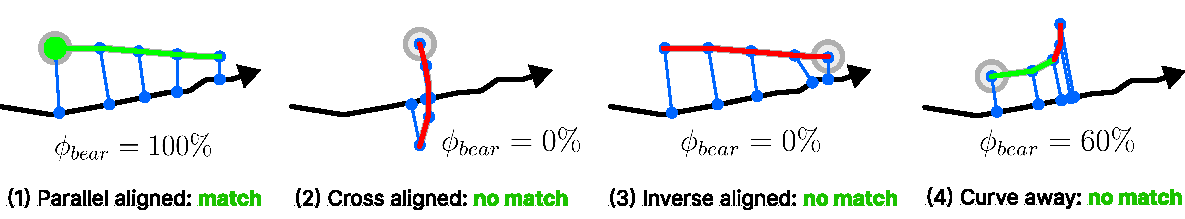
\includegraphics[width=\linewidth]{images/sg-selection-bearing-filter-sum.pdf}
\caption{Examples for (cumulative) bearing matching.}
\label{fig:sg-selection-bearing-filter-sum}
\end{figure}

\Cref{fig:sg-selection-bearing-filter-sum} gives an intuition for the final working principle of the bearing filter. In example (1) all segments of the signal's geometry are sufficiently aligned to the route. Examples (2) and (3) depict cases where none of the segments are within the angular threshold $t_{bear}$. Example (4) highlights a case where the first 60\% of the traffic light geometry matches the route. In the illustration, $t_{bear\_sum}$ is assumed to be larger than 60\%, and so the traffic light that curves away is filtered out. The higher this threshold is configured, the more aggressively the filter excludes inclined geometries.

\paragraph{Step 3 -- Length Filter:} With the previous two steps, we have two bearing thresholds ($t_{bear}$ and $t_{bear\_sum}$) in addition to the distance threshold $t_{dist}$. However, during the systematic testing of the thresholds it quickly became clear that these thresholds alone are not nearly enough to sufficiently distinguish matching from non-matching signals. During the search for other characteristics that distinguish matching from non-matching signals, a key observation was made: Non-matching traffic light geometries often have a shorter projection onto the route relative to their original length. This feature is also related to the traffic light geometry's angular position to the route but incorporates the shape of the route in between projected traffic light geometry coordinates.

\begin{figure}[htbp]
\centering
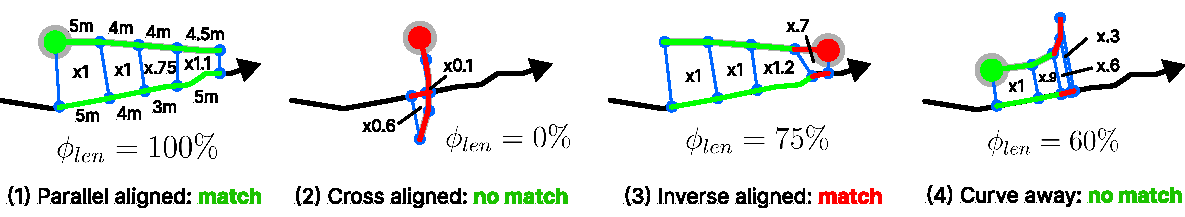
\includegraphics[width=\linewidth]{images/sg-selection-length-filter-sum.pdf}
\caption{Examples for (cumulative) length matching.}
\label{fig:sg-selection-length-filter-sum}
\end{figure}

To mathematically represent this intuition, a cumulative score $\phi_{len}$ is calculated similarly to the bearing filter and then subjected to a threshold $t_{len\_sum}$. The score $\phi_{len}$ quantifies the difference from 0 (no matching segments) to 1 (all segments matching), again weighted by the length of each segment. Example (3) shows that the length filter is not good at detecting inversely aligned geometries. However, since the bearing filter is assumed to handle this case, the length filter will likely not encounter such constellations.

Due to the similarity with the bearing filter, we can reuse its formulas and only have to replace the metric $\Psi$, which determines whether a segment is counted as a match. First, each segment $(c_1, \dots, c_n)$ is again projected onto the route as $(\bar{c_1}, \dots, \bar{c_n})$. Then, the length diff $\bar{\Delta}_{len_1}$ for the i-th segment is calculated as:

\begin{equation}
    \bar{\Delta}_{len_i} = 
        \begin{cases}
            0,& \text{if } line\_dist(\bar{c}_i, \bar{c}_{i+1}) = 0 \\
            abs(\frac{dist(c_{i}, c_{i+1})}{line\_dist(\bar{c}_{i}, \bar{c}_{i+1})}),              & \text{otherwise}
        \end{cases}
\end{equation}

where $dist$ is calculated as the Euclidean distance, and $line\_dist(\bar{c}_i, \bar{c}_{i+1})$ represents the distance along the route's geometry between $\bar{c}_i$ and $\bar{c}_{i+1}$. To calculate $line\_dist$, it is necessary to interpolate along the route's geometry. Using the calculated length diff, each segment of the signal's geometry is mapped as:

\begin{equation}
\Psi_{len_i} = 
    \begin{cases}
            1,& \text{if } \bar{\Delta}_{len_{i}} \in \left(1 - t_{len}, 1 + t_{len}\right)\\
            0,              & \text{otherwise}
        \end{cases}
\end{equation}

where $\Psi_{len_i} = 1$ means the segment matches the length diff threshold $t_{len}$. Finally, the weighted sum of all traffic light geometry segments is calculated as follows:

\begin{equation} 
\phi_{len} = 
    \underbrace{\sum_{i=1}^{n-1} 
    \frac{\Psi_{len_i}}{dist(c_i, c_{i+1})}}_{\text{Sum of matching segment lengths}}
    \times
    \underbrace{(\sum_{i=1}^{n-1} dist(c_i, c_{i+1}))^{-1}}_{\text{Sum of segment lengths}}
\end{equation}

Here, $\phi_{len} = 0$ means that all of the traffic light geometry's segments are shortened too much when projecting them onto the route geometry, indicating a traffic light that is not aligned with the route. Likewise, $\phi_{len} = 1$ means that all segments roughly stay the same length when projected onto the route. To distinguish when a traffic light is counted as a match or not, the thresholds $t_{len}$ and $t_{len\_sum}$ can be optimized accordingly.

\paragraph{Step 4 -- Overlap Matcher:} The previous matching steps often struggle with one particular problem: multiple parallel-aligned signals. Often, this case leads to a multi-selection of these signals, while only one of them will be taken by the cyclist. On the other hand, especially on complex intersections, there may be multiple consecutive traffic lights whose geometries partially overlap along the route but are still a valid match. Thus, some overlaps need to be filtered out, while others are intentional.

\begin{figure}[htbp]
\centering
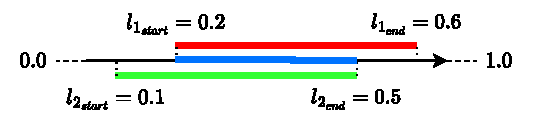
\includegraphics[width=0.5\linewidth]{images/overlap.drawio.pdf}
\caption{Example overlap.}
\label{fig:sg-matching-overlap-filter}
\end{figure}

First, the overlaps between traffic lights with respect to the route are determined. To accomplish this, the signals' geometries are snapped onto the route. As a result, each signal's start and end points along the route are determined, as highlighted in \Cref{fig:sg-matching-overlap-filter}. For each pair of matched traffic light geometries $(l_1, l_2)$, an overlap percentage $\phi_{overlap}$ is calculated as:

\begin{equation}
    \phi_{overlap} = \frac{min(l_{1_{end}}, l_{2_{end}}) - max(l_{1_{start}}, l_{2_{start}})}{max(l_{1_{end}}, l_{2_{end}}) - min(l_{1_{start}}, l_{2_{start}})}
\end{equation}

In the error case that the denominator is zero, $\phi_{overlap}$ is also mapped to zero. As soon as this percentage exceeds a threshold $t_{overlap\_pct}$, a decision process between both geometries is initiated:

\begin{enumerate}
    \item According to the traffic light metadata, if one of the traffic lights is a dedicated bike signal, choose that one.
    \item If one of both traffic lights perfectly matches the route, select that one. To determine whether a traffic light perfectly matches the route, a distance threshold $t_{perfect\_match}$ is configured.
    \item If both traffic lights are on different sides of the route and the distance between both traffic lights is smaller than a threshold $t_{road\_side}$, prefer the ordinary traffic side (in Germany, right-hand traffic). Whether a traffic light is left or right from the route is determined through $\bar{\Delta}_{bear_{i=1}}$.
    \item Otherwise, decide purely by the distance to the route.
\end{enumerate}

The thresholds $t_{overlap\_pct}$, $t_{perfect\_match}$, and $t_{road\_side}$ can be used to tune the final result. In the case of $\phi_{overlap} < t_{overlap\_pct}$, both traffic lights are kept. This allows for intentional small overlaps at complex intersections without filtering one of both traffic lights out.

\begin{table}[h]
\caption{Summary of thresholds and search space.}
\begin{tabular}{@{}lp{8cm}l@{}}
\toprule
\textbf{Hyperparameter}  & \textbf{Explanation} & \textbf{Search Interval} \\
T1 ($t_{dist}$) & Traffic light geometries must be within this distance of the route. & $[1m, 100m]$ \\
T2 ($t_{bear\_sum}$) & The minimum proportion of the signal's geometry matching $t_{bear}$. & $[0, 100\%]$ \\
T3 ($t_{bear}$) & If segments of the traffic light geometry are angled more steeply to the route than this value, they are not counted for $t_{bear\_sum}$. & $[0°, 180°]$ \\
T4 ($t_{inv}$) & Whether inverted traffic light geometries should be matched. & $[\text{False}, \text{True}]$ \\
T5 ($t_{len\_sum}$) & The minimum proportion of the signal's geometry matching $t_{len}$. & $[0, 100\%]$ \\
T6 ($t_{len}$) & If segments of the traffic light geometry are elongated or shortened more than $1 \pm t_{len}$ when projected onto the route, they are not counted for $t_{len\_sum}$. & $[0, 1]$\\
T7 ($t_{road\_side}$) & If two overlapping traffic lights are on opposite sides of the route and less than this distance away from each other, decide by the ordinary traffic side. & $[0, 100m]$ \\
T8 ($t_{perfect\_match}$) & If a signal's geometry is closer to the route than this value, it is preferred over another overlapping traffic light geometry. & $[0, 50m]$ \\
T9 ($t_{overlap\_pct}$) & If two traffic lights overlap more relative to their combined length, a decision process between both traffic lights is initiated. & $[0, 100\%]$ \\
\bottomrule
\end{tabular}
\label{tab:hyperparameter-space}
\end{table}

\paragraph{Model Finetuning:} The designed filtering pipeline has several thresholds that must be carefully selected to optimize the final matching performance. Here, it is important to consider that each filter influences the subsequent filters in the pipeline. This means that it is difficult and time-intensive to tune the individual filters by hand. A solution to this problem is utilizing a hyperparameter tuning algorithm, which tries to understand the influence of each hyperparameter on a model and maximizes its score. This algorithm can run overnight, resulting in a proposed model configuration after a few hundred to thousand trials. To prepare the model for hyperparameter tuning, search spaces for each hyperparameter must be defined. These search spaces are summarized in \Cref{tab:hyperparameter-space}. The Tree-Structured Parzen Estimator hyperparameter tuning algorithm \cite{ozaki_multiobjective_2020} is utilized to find a good configuration on the ground truth benchmark. The objective function given to the tuner algorithm is the F1 score.

\subsection{Machine Learning Filtering Approach}

One identified problem of the algorithmic approach is that each threshold is defined globally and equally applied to all situations. However, not all intersections are crossed similarly by routes. Thus, the filtering pipeline would be applied too strictly in some situations, while the thresholds are not applied strictly enough in others. Here, an ML model can be useful to employ a more flexible and interlinked mapping of the geometric properties.

Regarding the problem of deciding between "match" and "no match" for each traffic light geometry, there may be many creative ways to establish an ML classifier. For example, it would be possible to generate top-down images of each intersection and utilize machine-learning techniques from image detection or segmentation to classify each signal. However, as a rule of thumb, more complicated tasks tend to require larger ML models, which in turn require a larger ground truth. 

Unfortunately, the ground truth itself would ever be able to contain a few thousand unique samples at most, which speaks against the viability of applying more advanced deep learning models. Dataset augmentation through artificial distortion of the traffic light geometries was found in preliminary experiments not to be a purposeful option. A meaningful balance between marginally distorting the traffic light geometries and invalidating the labeling could not be identified. Furthermore, there would be the concern of scalability with larger models and a more complex feature processing pipeline. Thus, the decision was made to opt for a more conservative approach.

\begin{figure}[htbp]
\centering
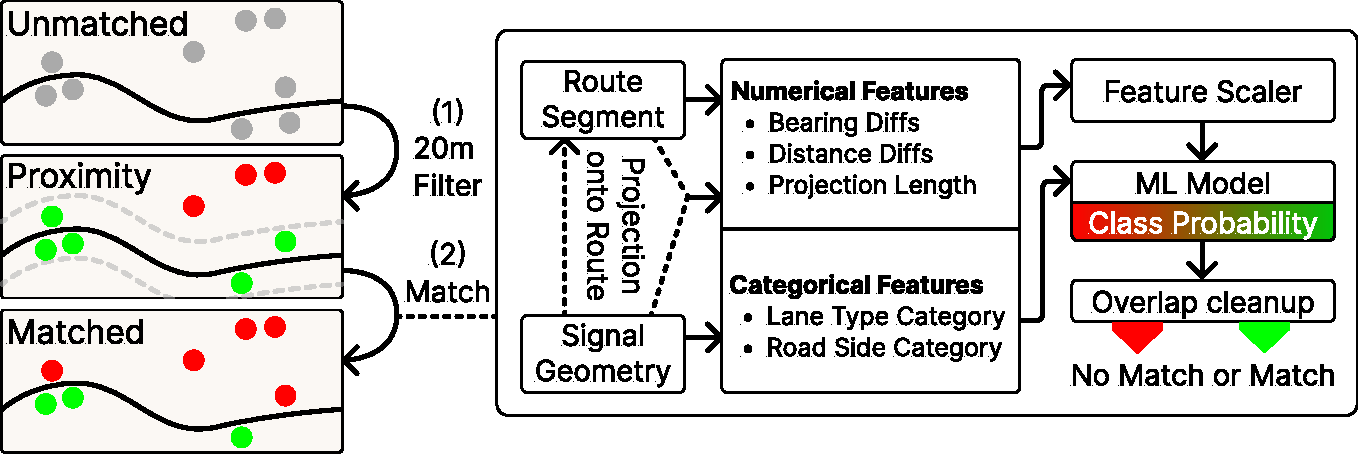
\includegraphics[width=\linewidth]{images/sg-matching-ml-model.pdf}
\caption{Filtering steps for matching with the ML model.}
\label{fig:sg-matching-ml-model}
\end{figure}

The proposed approach (see \Cref{fig:sg-matching-ml-model}) operates as follows: The bearing, length, and overlap filtering steps from the algorithmic approach are removed and replaced with a single "Match" step to incorporate the ML classifier into the filtering process. During this step, the signal's geometry is first projected onto the route. The result of this step is one sample incorporating the traffic light geometry and the projected traffic light geometry onto the route. It is important to note here that each sample considers one signal, not a complete intersection. Based on the sample, numerical and categorical features are calculated that represent the geometrical relationship between the route and the traffic light geometry.

The numerical features are subjected to a feature scaler to prepare them for model inference. The categorical features are calculated or extracted from the traffic light metadata. Both numerical features and categorical features are input into the ML model. As a result, the ML model produces a class probability for "match" or "no match." The class probability is utilized in an additional overlap cleanup step (similar to the algorithmic approach's overlap filter) to obtain the final matching traffic lights along the route.

\paragraph{Feature and Model Grid Search:} To select a suitable ML model architecture and feature processing pipeline, gathered experiences from hyperparameter tuning were utilized to systematically and rigorously identify promising configurations. Out of the tested traditional model architectures including k-Nearest-Neighbors (k-NN), Decision Tree, Random Forest, Multilayer Perceptron (MLP), AdaBoost, Gaussian Naive Bayes, Quadratic Discriminant Analysis (QDA), and Support Vector Machine (SVM), the MLP model overall performed the best and was thus selected as the final classifier, after testing other promising models with different feature constellations. 

To ensure comparability during the model testing process, each model feature pipeline was trained and tested using the stratified variant of the k-fold cross-validation\footnote{\url{https://scikit-learn.org/1.3/modules/generated/sklearn.model_selection.StratifiedKFold.html}}. As there are many more non-matching traffic lights along routes in the ground truth than matching signals, this variant ensures that a similar balance is present in each generated training/testing split of the ground truth dataset. By looking at the models' scores and the mutual information of each feature, some features were discarded as they provided no additional information. The final feature set is as follows:

\begin{itemize}
    \item The lane type of the signal. This property is extracted from the signal's metadata and one-hot-encoded.
    \item The road side of the signal. To calculate this property, it is determined on which side of the route the first coordinate of the traffic light geometry is located.
    \item The maximum and minimum bearing diffs between the traffic light geometry segments and their projections onto the route ($\bar{\Delta}_{bear_i}$).
    \item The change in route bearing from the first to the last route segment. 
    \item The first, last, and shortest distance between traffic light geometry coordinates and their projections onto the route.
    \item The length of the traffic light geometry's projection onto the route.
\end{itemize}

A feature scaling algorithm is employed to optimize the ML model's learning and inference process. Here, it is usually a good option to choose a Yeo-Johnson power transformation \cite{yeo_new_2000}, which includes standardization and additionally tries to symmetrize the observed data into a normal distribution. Together with the scaled numerical features, the one-hot-encoded categorical features are input into the model as, in sum, 16 features. Together with the model, the parameters of the Yeo-Johnson power transformation are only fit to the dataset's training proportion.

\begin{figure}[htbp]
\centering
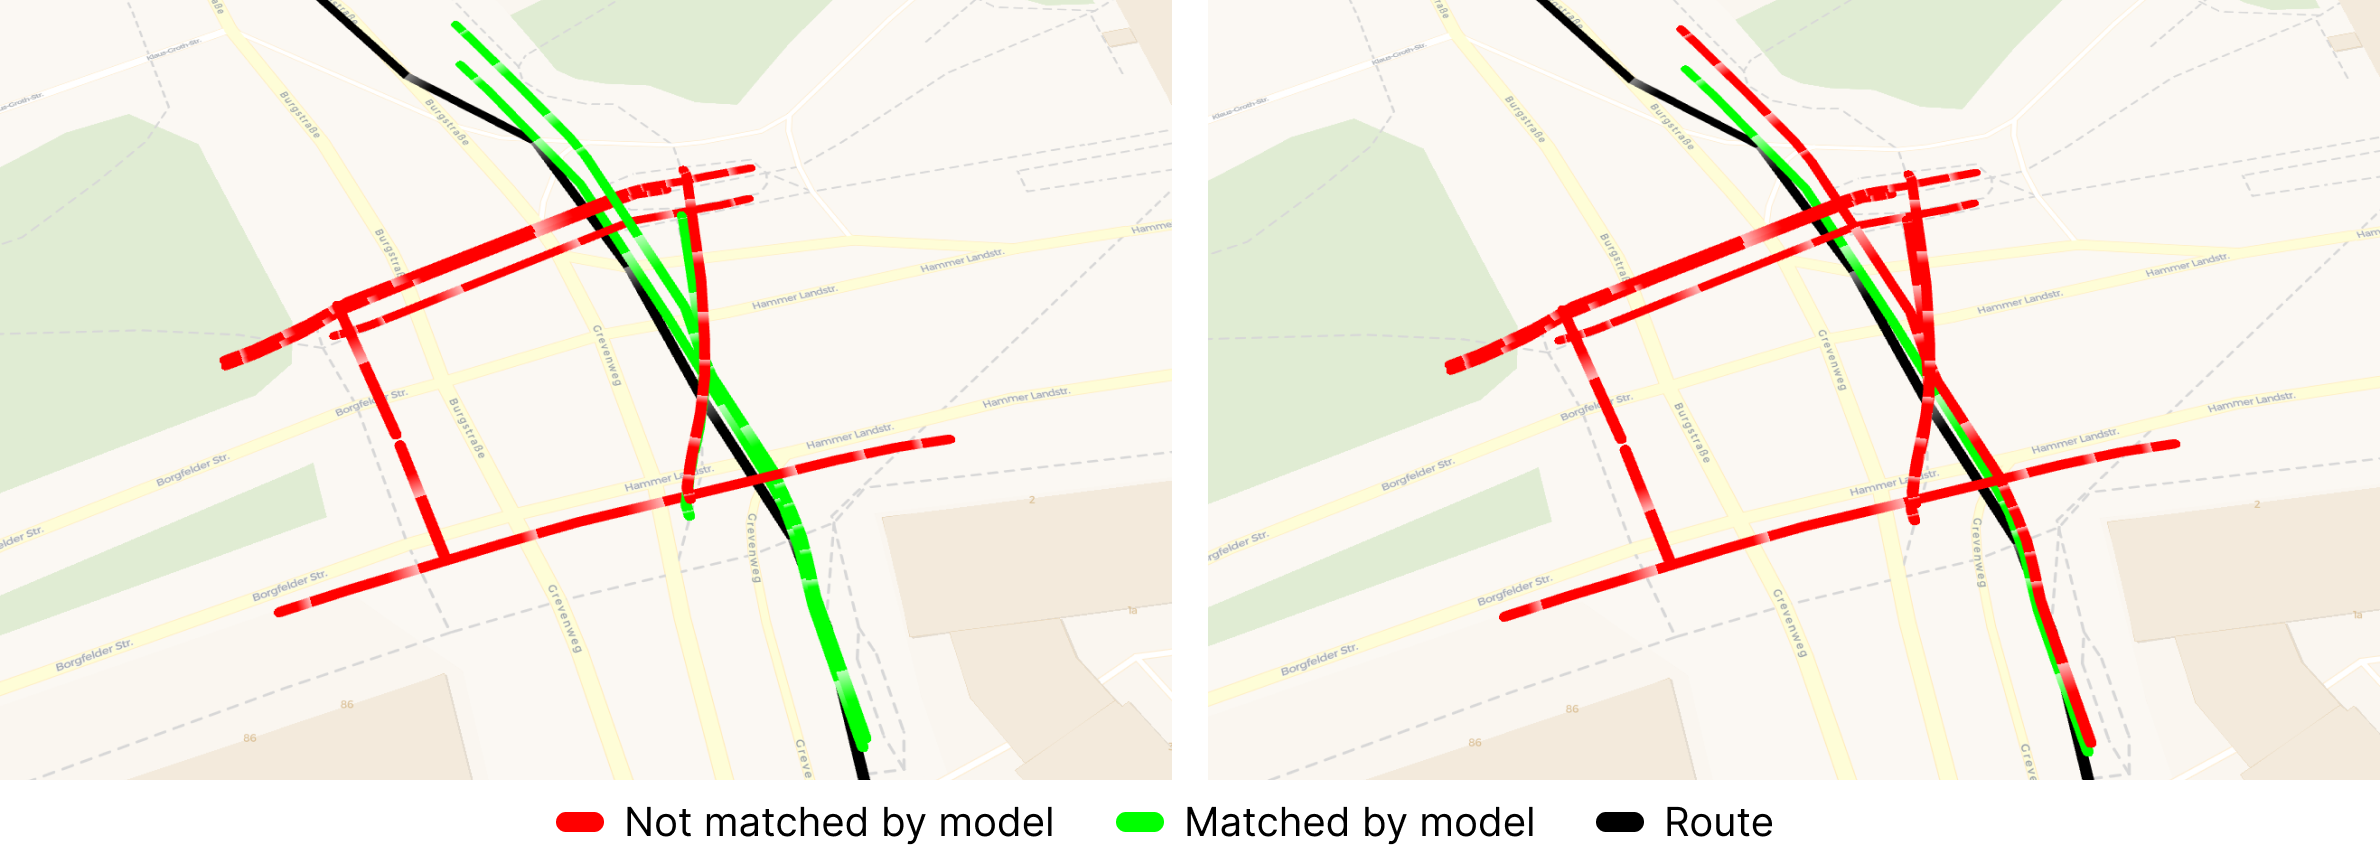
\includegraphics[width=\linewidth]{images/sg-selection-overlap-cleanup.png}
\caption{Model selection without (left) and with (right) overlap cleanup.}
\label{fig:sg-selection-overlap-cleanup}
\end{figure}

\paragraph{Overlap Cleanup:} As in the algorithmic approach, there may be some cases where multiple overlapping traffic lights are selected. These duplicate selections may happen when multiple traffic light geometries are very closely aligned to the route, and must be cleaned up, as the app should only focus on the most likely used signal. 

As shown in \Cref{fig:sg-selection-overlap-cleanup}, the utilized traffic light is most likely the longest of the three selected geometries. This traffic light arguably has the best alignment with the route geometry. How much the model thinks a traffic light matches the route can be measured by the output probability (neuron activation) for the two classes "match" and "no match." This feature is used to force the model to decide between overlapping signals. In case a sufficient overlap between two traffic light geometries is detected, the traffic light with the higher probability for "match" is selected. As highlighted in \Cref{fig:sg-selection-overlap-cleanup}, this process is effective at filtering out the problem.

\subsection{Integration of Unconnected Intersections}

Not all intersections have traffic lights connected to Hamburg's data broker. However, this represents a problem for matching traffic lights along a route. If an unconnected intersection lies between the user and the next connected intersection, the user may get a speed advisory for the wrong intersection. Although the traffic light is later visualized on the in-app map, this may still lead to confusion for the user. Thus, it is crucial also to identify the unconnected intersections along the bike path. These unconnected intersections are later visualized with a unique traffic light symbol in the user interface.

To find out which intersections are not connected to the system (but still signalized), the Lichtsignalanlagen Hamburg\footnote{\url{https://metaver.de/trefferanzeige?docuuid=C498DEED-985C-11D5-889E-000102B6A10E}} dataset is utilized. This dataset is updated periodically every four months and contains single coordinates of each signalized intersection in Hamburg. Thus, the dataset does not resolve individual traffic light geometries but the center locations of the intersection node. 

To identify which intersections are connected, it is determined which intersections have traffic light geometries within an empirically defined threshold of 50 meters. These intersection nodes from the Lichtsignalanlagen Hamburg dataset are marked as "connected." All other nodes are marked as "unconnected." In case of a traffic light unassigned to any intersection node, it is assumed that this intersection node is missing in the Lichtsignalanlagen Hamburg dataset, and a new intersection node is created. 

Finally, a list of intersection nodes is matched to the route by a distance threshold of 50 meters. To avoid displaying a speed advisory for a wrong intersection, the app handles each unconnected intersection like a traffic light that doesn't send any data. Once an unconnected intersection is passed before another (connected) signal, the speed advisory is enabled again. This step completes the traffic light matching pipeline.

\begin{Summary}[Summary of Methods]
Route-based traffic light matching is proposed as a novel solution to the problem of identifying traffic lights for GLOSA. The proposed method is designed to be practical for all smartphone mounting spots and invulnerable to inaccurate GNSS. Furthermore, all upcoming traffic lights are known at any time during the ride. However, a significant challenge is to precisely estimate which sequence of traffic lights will most likely be utilized by a cyclist. The approach must employ human-like spatial reasoning to tell apart non-matching from matching signals.

To develop and test mathematical models with the goal of resembling human spatial reasoning, human matchings of traffic lights along randomized routes are collected through a web tool. The resulting ground truth dataset is utilized to calculate an overall matching quality through the F1 score.

Multiple methods were tested preliminarily but not investigated further. Nonetheless, the learnings from these methods were ultimately incorporated into an algorithmic filtering pipeline. This pipeline employs geometrical filters that calculate each signal's distance, bearing, and projection length to determine whether it would suit the route. Finally, overlapping traffic lights are compared to each other to decide which one matches the route better. As a result, a sequence of traffic lights is returned, which are predicted to match a given input route.

To further improve the developed filtering pipeline, it was determined that the geometric features, such as bearing or projection length, could be weighted more dynamically by an ML model. The final MLP model utilizes 16 features calculated from the signal's geometry and its projection onto the route to determine if this traffic light matches the route. In case of overlaps, the traffic light predicted to match the route most likely is chosen.

Finally, to avoid speed advisories being given for a traffic light that comes after an unconnected but signalized intersection, the Lichtsignalanlagen Hamburg dataset is utilized. 
\end{Summary}

\section{Results}

The evaluation of the traffic light matching process is divided into several parts. We begin with the data analysis of traffic light geometries and then proceed to examine the Ground Truth. We assess whether the Ground Truth is representative enough to make qualified statements about the accuracy of the developed procedures. Using these considerations, we then evaluate the benchmark performance of both approaches. Additionally, we investigate how effectively both methods select the correct traffic lights, even in the presence of routing errors. The matching time and practicality of the final model are examined through a short performance analysis on a TU-Dresden deployment. Finally, we validate our benchmark results through a test in Hamburg.

\subsection{Study of Traffic Light Geometries in Hamburg}

Initiating the evaluation, we first take a closer look at traffic light geometries. The concept emphasizes that meta-information about the modes of transportation served by a traffic light is a crucial decision criterion. The developed procedure should consistently choose a dedicated bicycle traffic light when feasible based on the intersection topology. Thus, it is vital to understand the spatial distribution and shape patterns of bicycle traffic light geometries.

As of December 8, 2023, 85.6\% of the 791 available intersection nodes in the system have at least one dedicated bicycle traffic light. At 24.5\% of intersections, there is at least one traffic light shared between cyclists and motor vehicles, and 6.7\% have lights designated for mixed traffic involving cyclists, motor vehicles, and buses. 3\% of intersections feature lights shared between pedestrians and cyclists.

\begin{figure}[t]
\centering
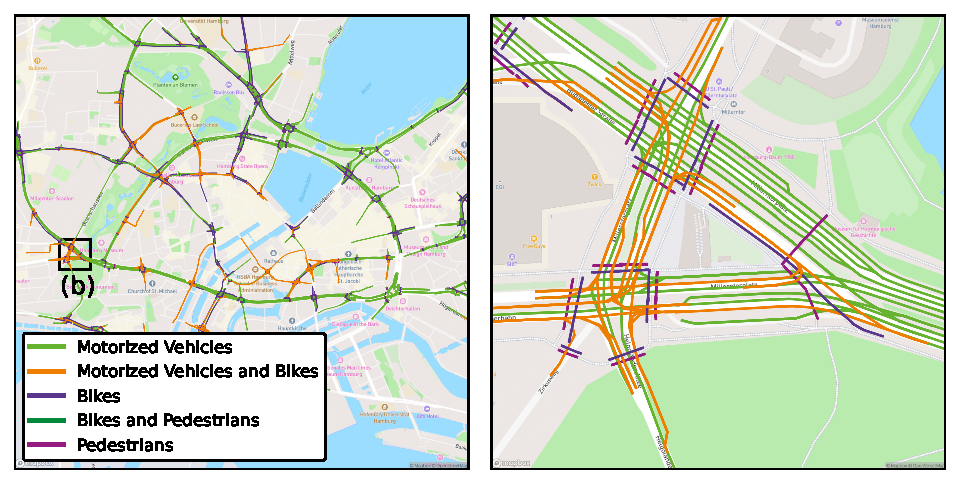
\includegraphics[width=\linewidth]{images/lanes-map.pdf}
\caption{Types of transport modes served by traffic lights as extracted from metadata.}
\label{fig:lanes-map}
\end{figure}

As shown in \Cref{fig:lanes-map}, the percentage overlap occurs because there are often multiple parallel traffic lights per intersection and direction, providing theoretical choices for cyclists, but only one ultimately proves to be the optimal option. Examining individual ingress lanes and potential turns from these lanes reveals that cyclists frequently have numerous options to turn in the same direction. Out of a total of 4349 marked ingress lanes for cyclists, 653 (15\%) of these lanes are associated with multiple signal geometries. For instance, at intersection 177 located at 53°34'10.6"N 10°03'22.1"E, cyclists can turn right into four lanes, left into four lanes, and proceed straight from a single ingress lane.

While multiple connections typically operate simultaneously, and an incorrect choice does not necessarily lead to a wrong speed recommendation, it is essential to consider that different turning directions may be served by separately operating signal controllers.

In cases where the selection is solely based on the next signal geometry due to the precise overlap of ingress lanes, ambiguity arises, necessitating the display of multiple parallel lanes in the user interface. Additionally, there are often several parallel ingress lanes, which can be independently controlled, such as a bicycle signal preceding a vehicle signal also tagged for cyclists. Although these lanes do not physically overlap, they are usually situated a few meters apart.

\begin{figure}[htbp]
\centering
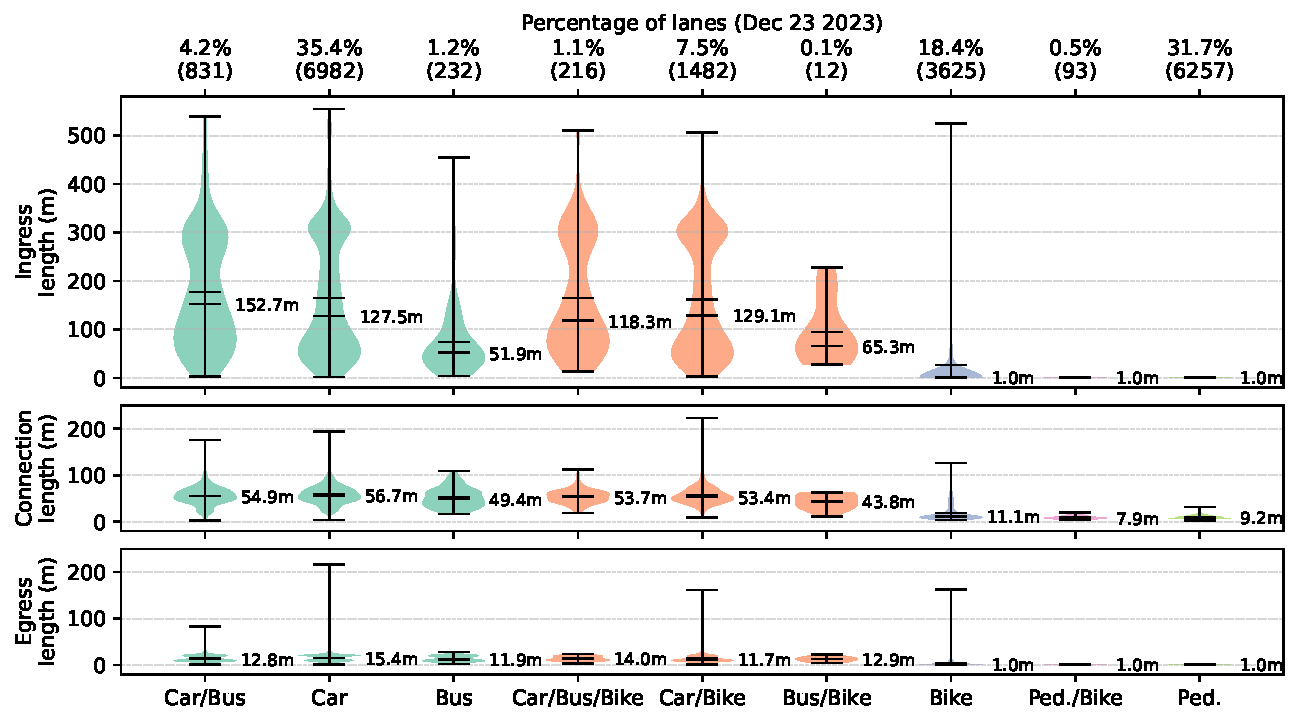
\includegraphics[width=\linewidth]{images/lanes-lengths.pdf}
\caption{Lane lengths of traffic lights in Hamburg as measured through the Vincenty distance.}
\label{fig:ingress-lane-lengths}
\end{figure}

Another challenge is the issue of ingress lane length. As depicted in \Cref{fig:ingress-lane-lengths}, it is generally reasonable to assume a non-too-short ingress lane length for cars and use it for matching. However, contrary to Stahlmann et al.'s report (2018) \cite{stahlmann_exploring_2018}, link lengths of 590 to 910 meters cannot be observed. Even when summing ingress lane, connection, and exit lane geometries, the total length is well below 300 meters. Therefore, it is crucial to utilize additional map data to artificially extend ingress lane lengths and activate a speed recommendation service in a timely manner.

For cyclists, the situation is quite different. As initially described, the issue for cyclists is that many traffic lights can be approached from multiple directions. The result is visible in \Cref{fig:ingress-lane-lengths}, with ingress lane lengths, if all (including shared) bicycle lanes marked in the diagram are considered together, having a median length of 1 meter. In many cases, ingress lanes would need to be artificially extended in multiple directions, or at least multiple longer ingress lanes would need to be provided. This would require a restructuring of all intersection topologies.

Even then, the problem is not entirely resolved, as the ingress lanes of multiple traffic lights would overlap, leading to an unclear mapping of which traffic light the user is approaching. In summary, these results confirm the observation that any location-based matching method without knowledge of the actual turn taken at the upcoming intersection is severely limited for cyclists. The ambiguity in approaching the traffic light would be too significant in many cases to make a clear selection, even assuming perfect GNSS accuracy.

\subsection{Analysis of Ground Truth}

The development of the route-based matching method involved creating several ground truths, which we will now examine in more detail.

\begin{figure}[htbp]
\centering 
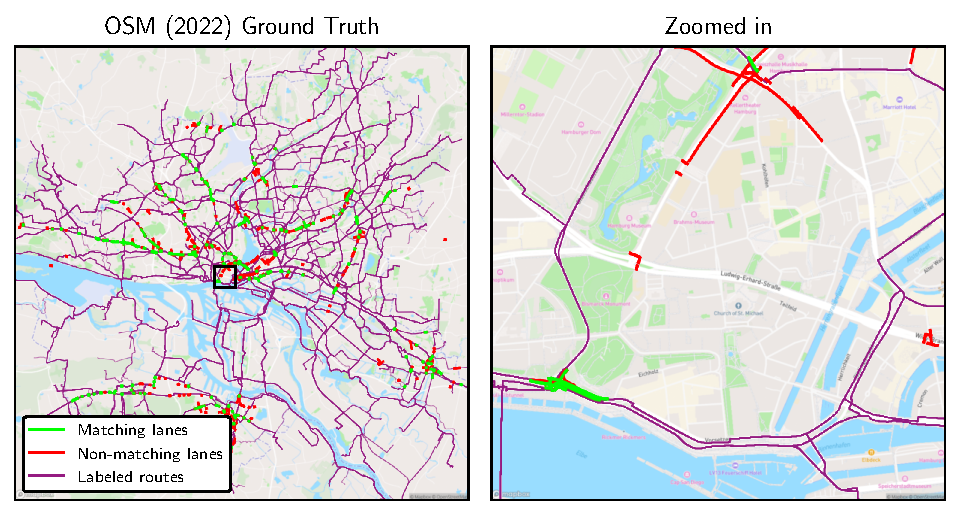
\includegraphics[width=\linewidth]{images/matching-ground-truth-osm-old.pdf}
\caption{OpenStreetMap 2022 ground truth for model training and evaluation.}
\label{fig:matching-ground-truth-osm-old}
\end{figure}

The first ground truth was established in 2022 and consists of 148 randomly generated bicycle routes through Hamburg using OSM and the GraphHopper \texttt{bike2} profile. This ground truth is illustrated in \Cref{fig:matching-ground-truth-osm-old}. The ground truth was constructed using a dataset of traffic light geometries containing 2414 individual connections available in 2022. A total of 1043 traffic lights were manually assigned to the 148 routes. On average, each route encompasses seven traffic lights.

In \Cref{fig:matching-ground-truth-osm-old}, the manually assigned traffic lights (in blue) are marked in green, while traffic lights that were never assigned are marked in red. It is noticeable that there are some traffic lights that were never selected. This originates from two reasons: some intersections were not traversed by any generated route, and at traversed intersections, there are often traffic lights that never constitute a meaningful match. In extreme cases, there are intersections where no traffic light matches the route, perhaps because it is not relevant to the bike path alongside the road.

Along the 148 routes, a total of 6440 connections were considered at least once during the labeling of the ground truth, with 5397 (83.8\%) marked as "no match." This pertains to all traffic lights within the 20m radius, which is always drawn around the route. Therefore, the matching method must label significantly more connections as "no match" in the matching process than as "match."

While only 549 unique connections are identified at least once as a "match," an additional 1231 unique connections are never identified as a "match" despite being considered. Consequently, the 2022 OSM dataset covers a total of 73.7\% (1780) of all 2414 traffic lights, although not necessarily accounting for all possible entry directions of the intersections.

\begin{figure}[htbp]
\centering 
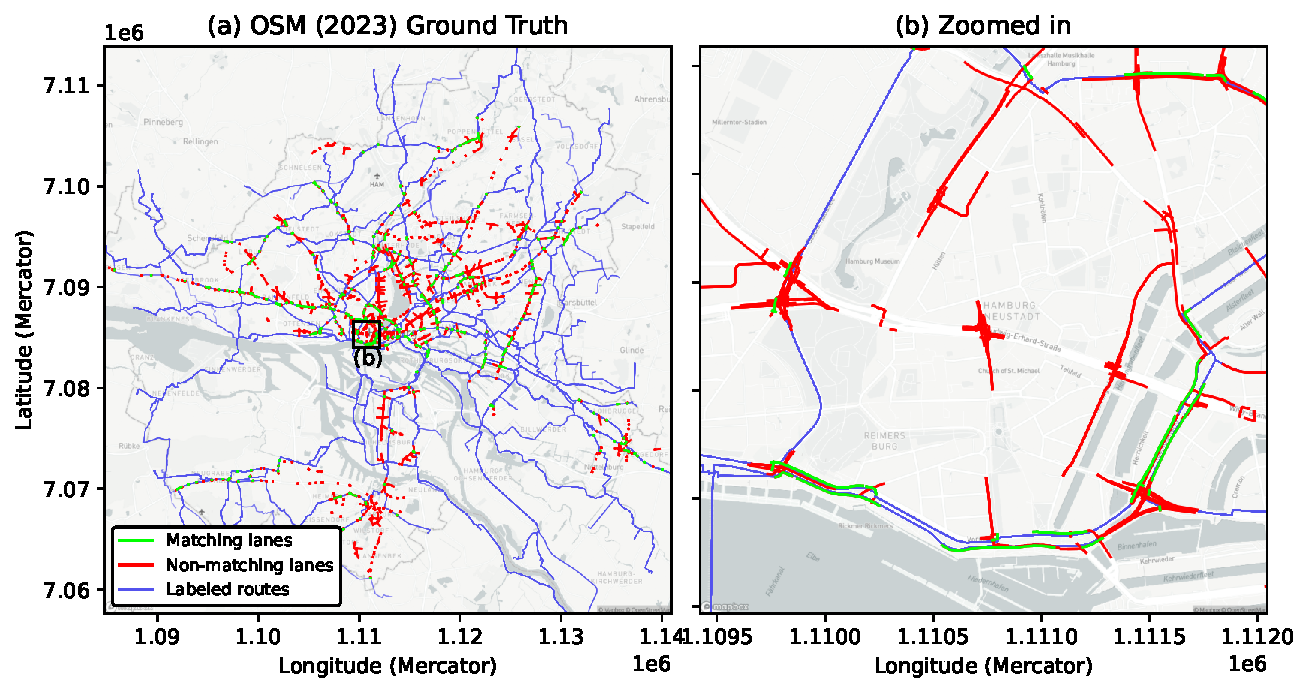
\includegraphics[width=\linewidth]{images/matching-ground-truth-osm.pdf}
\caption{Additional OpenStreetMap 2023 ground truth for model training and evaluation.}
\label{fig:matching-ground-truth-osm}
\end{figure}

A limitation of the first ground truth is its inclusion of only 2414 connections, representing 44\% of the 5486 connections available as of December 13, 2023.

To address this limitation, a second ground truth was created in 2023 to validate the models and results using the 2022 ground truth. This new ground truth contains 5168 connections, accounting for 94.2\% of the available connections, as depicted in \Cref{fig:matching-ground-truth-osm}. The 2023 ground truth consists of 52 routes generated using the same schema and 758 connections marked as "match." This equates to approximately 15 connections per route, maintaining consistency with the increased coverage.

Notably, the addition of new routes to the ground truth does not necessarily result in the addition of new connections. Since multiple routes can traverse an intersection in a similar manner, each newly added route tends to contribute fewer new traffic lights to the dataset.

An implication of this is that there is a limit to the number of routes that can be meaningfully added to the dataset. With each new route, there is an increased risk of introducing duplicate examples. Excessive duplicates should be avoided to minimize dataset bias. Specifically, when training an ML classifier, an abundance of duplicates can lead to overfitting and reduced generalization capability.

\begin{figure}[htbp]
\centering 
\begin{tabular}{cc}
\footnotesize{(a) Redundancy in OSM Ground Truth (2022)} & \footnotesize{(b) Redundancy in OSM Ground Truth (2023)} \\
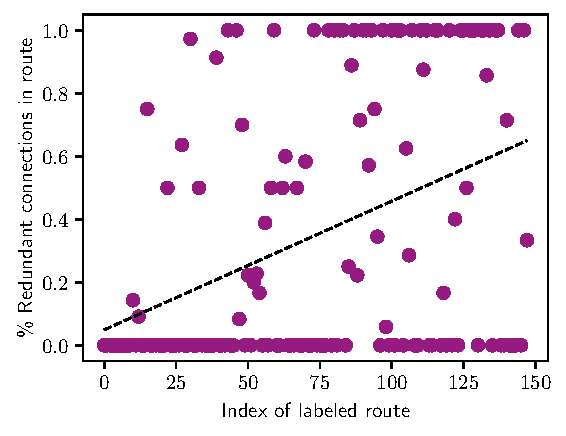
\includegraphics[width=0.45\linewidth]{images/matching-ground-truth-progression-osm-old.pdf} & 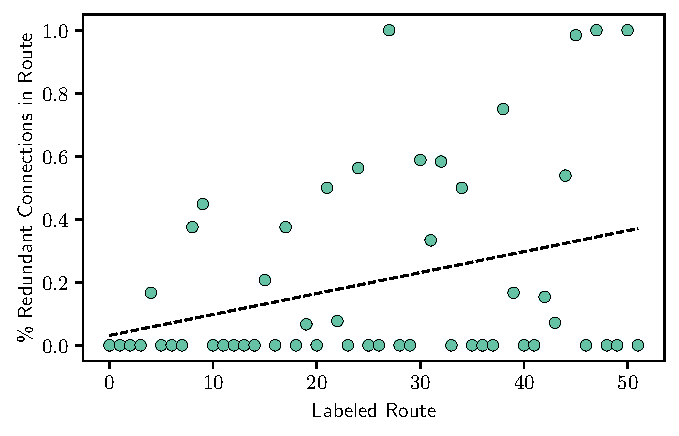
\includegraphics[width=0.45\linewidth]{images/matching-ground-truth-progression-osm.pdf} \\
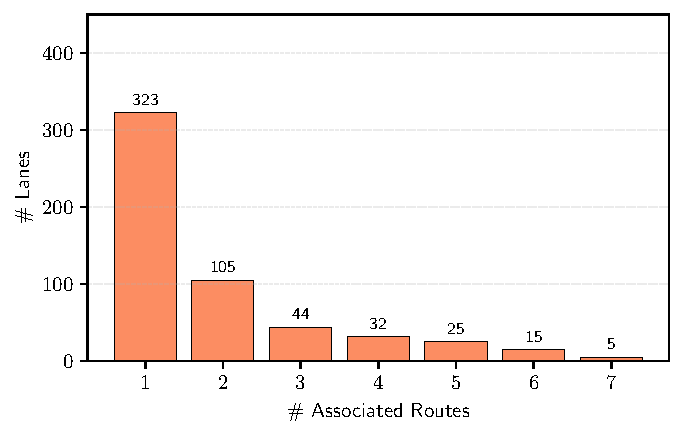
\includegraphics[width=0.45\linewidth]{images/matching-ground-truth-lsas-per-route-osm-old.pdf} & 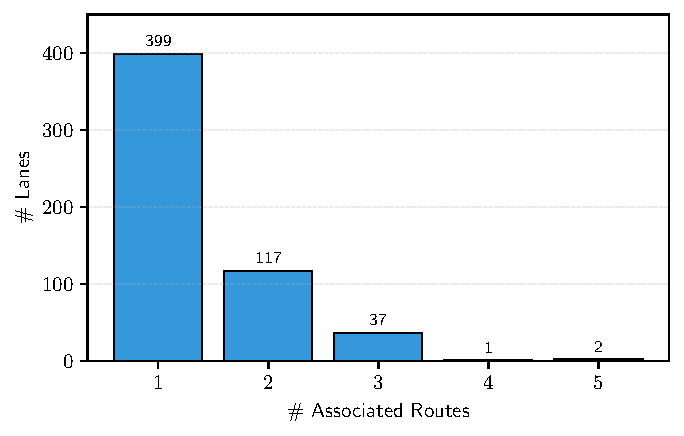
\includegraphics[width=0.45\linewidth]{images/matching-ground-truth-lsas-per-route-osm.pdf} \\
\end{tabular}
\caption{Redundancy of each ground truth as indicated by new constellations and multiple assignments to routes.}
\label{fig:ground-truth-routes-per-lanes-osm}
\end{figure}

The relationship is more precisely illustrated in \Cref{fig:ground-truth-routes-per-lanes-osm}. For each new route, it was determined how many "match"-marked connections already existed in the dataset. Since more routes were labeled in the 2022 OSM dataset than in the 2023 OSM dataset, the redundancy of new routes tends to be higher.

By examining the temporal trend of the percentage of redundant connections per new route, we can estimate the likelihood of encountering previously seen connections in a new random route. Assuming a linear relationship, as depicted by the dashed line in \Cref{fig:ground-truth-routes-per-lanes-osm}, the probability is 65\% for the 2022 OSM dataset and 38\% for the 2023 OSM dataset.

In conclusion, we cannot add an unlimited number of routes to the ground truth without encountering redundancy issues. The decision on where to terminate the creation of new routes is somewhat arbitrary. In the creation of the 2023 OSM dataset, this decision was made earlier than in the 2022 OSM dataset.

The result of this creation process is that most lanes (connections) are assigned to only one route. As shown in \Cref{fig:ground-truth-routes-per-lanes-osm}, this applies to 323 routes in the 2022 OSM dataset and 399 routes in the 2023 OSM dataset. In the 2022 OSM dataset, there are isolated lanes assigned to up to seven different routes.

The distribution overall indicates that there may be significantly more duplicates in the 2022 OSM dataset compared to the 2023 OSM dataset. Whether these duplicates are excessive cannot be accurately assessed without testing the model's generalization capability on unseen data, which we will address in detail in the next section.

\subsection{Model Evaluation}

\begin{table}[h]
\caption{Tuned hyperparameters for the algorithmic matching model.}
\resizebox{\linewidth}{!}{\begin{tabular}{@{}llllllllll@{}}
\toprule
\textbf{Ground Truth} & $t_{dist}$ & $t_{bear}$ & $t_{bear\_sum}$ & $t_{inv}$ & $t_{len}$ & $t_{len\_sum}$ & $t_{road\_side}$ &  $t_{perfect\_m.}$ & $t_{overlap}$ \\
  \midrule
  OSM (2022) & 20m & 33° & 79\% & False & 0.99 & 93\% & 59m & 50m & 43\% \\
  OSM (2023) & 19m & 50° & 78\% & False & 0.96 & 77\% & 95m & 46m & 5\% \\
\bottomrule
\end{tabular}}
\label{tab:hyperparameter-tuning-results}
\end{table}

Two models were designed: the algorithmic model and the ML model. Each model was trained and evaluated on the ground truths presented in the previous section. First, let's examine the algorithmic model. The same version of the algorithmic model was trained once on the 2022 OSM dataset and once on the 2023 OSM dataset. This resulted in two distinct models, each validated on the other dataset.

The specific model configurations are detailed in \Cref{tab:hyperparameter-tuning-results}. The hyperparameter tuning process selected similar values for the initial thresholds along the filter pipeline. Ignoring the parameters of the overlap matchers initially, notable differences are observed only in the chosen bearing threshold $t_{bear}$ and the length filter. While the 2023 model is less strict in filtering steeply angled lane geometries, the length filter is configured more rigorously. This is not surprising, as both the bearing filter and the length filter pertain to similar properties between the route and the lane. The overlap matcher, which comes last in the filter pipeline, exhibits relatively large differences between the two model variants. 

\begin{figure}[htbp]
\centering 
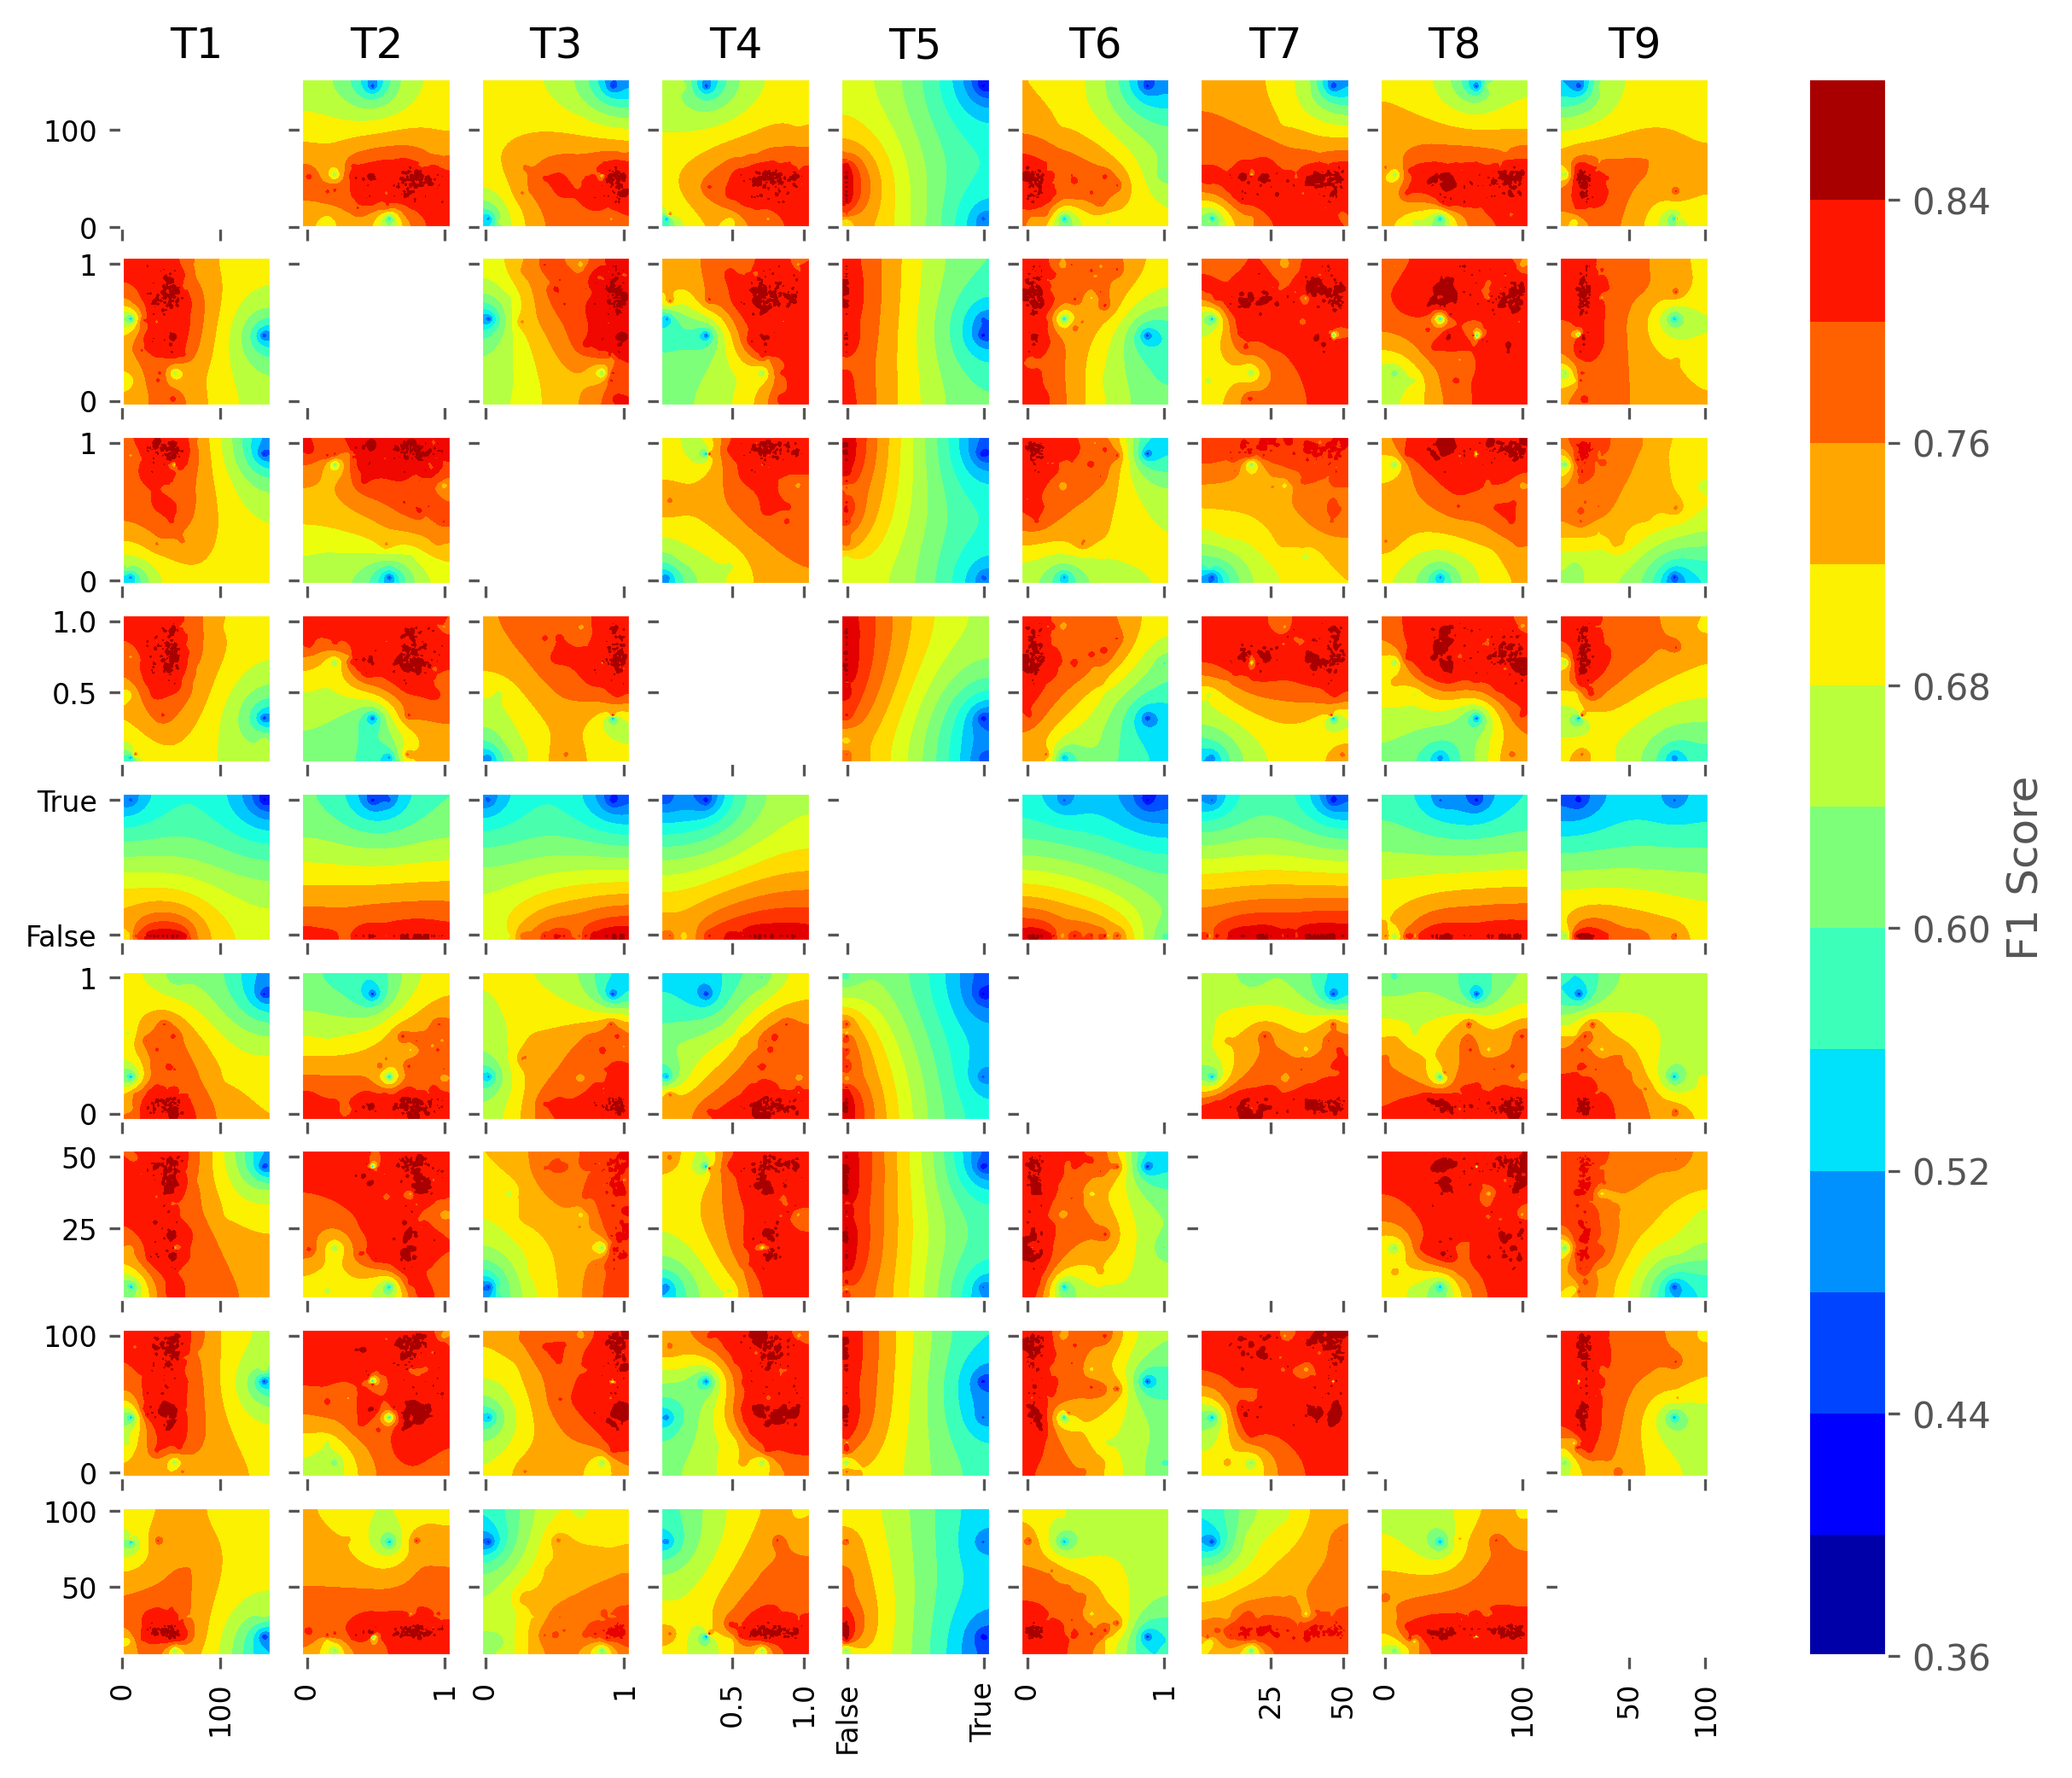
\includegraphics[width=\linewidth]{images/matching-hpt-contour-topological-osm-updated.png}
\caption{Contour plot of the hyperparameter tuner's threshold search space indicating its gradient measurements for F1 score optimization.}
\label{fig:hyperparameter-contourplot}
\end{figure}

\Cref{fig:hyperparameter-contourplot} provides more detailed insights into the interpretation of the hyperparameter tuner regarding the direction in which the parameter configuration needs to be optimized to achieve the maximum F1 score. This plot was generated using the training history of the 2023 model.

Several interesting conclusions can be drawn from the figure regarding the training and the general interpretation of a "good" match between a route and a traffic light geometry. Firstly, a clear trend is observed with Threshold 5, which decides whether inversely oriented traffic light geometries should be chosen as a match. The tendency is clearly towards "no," aligning with Rule 6 in the dataset creation, stating that traffic light geometries should never be chosen against the direction of travel. 

\begin{figure}[H]
\centering 
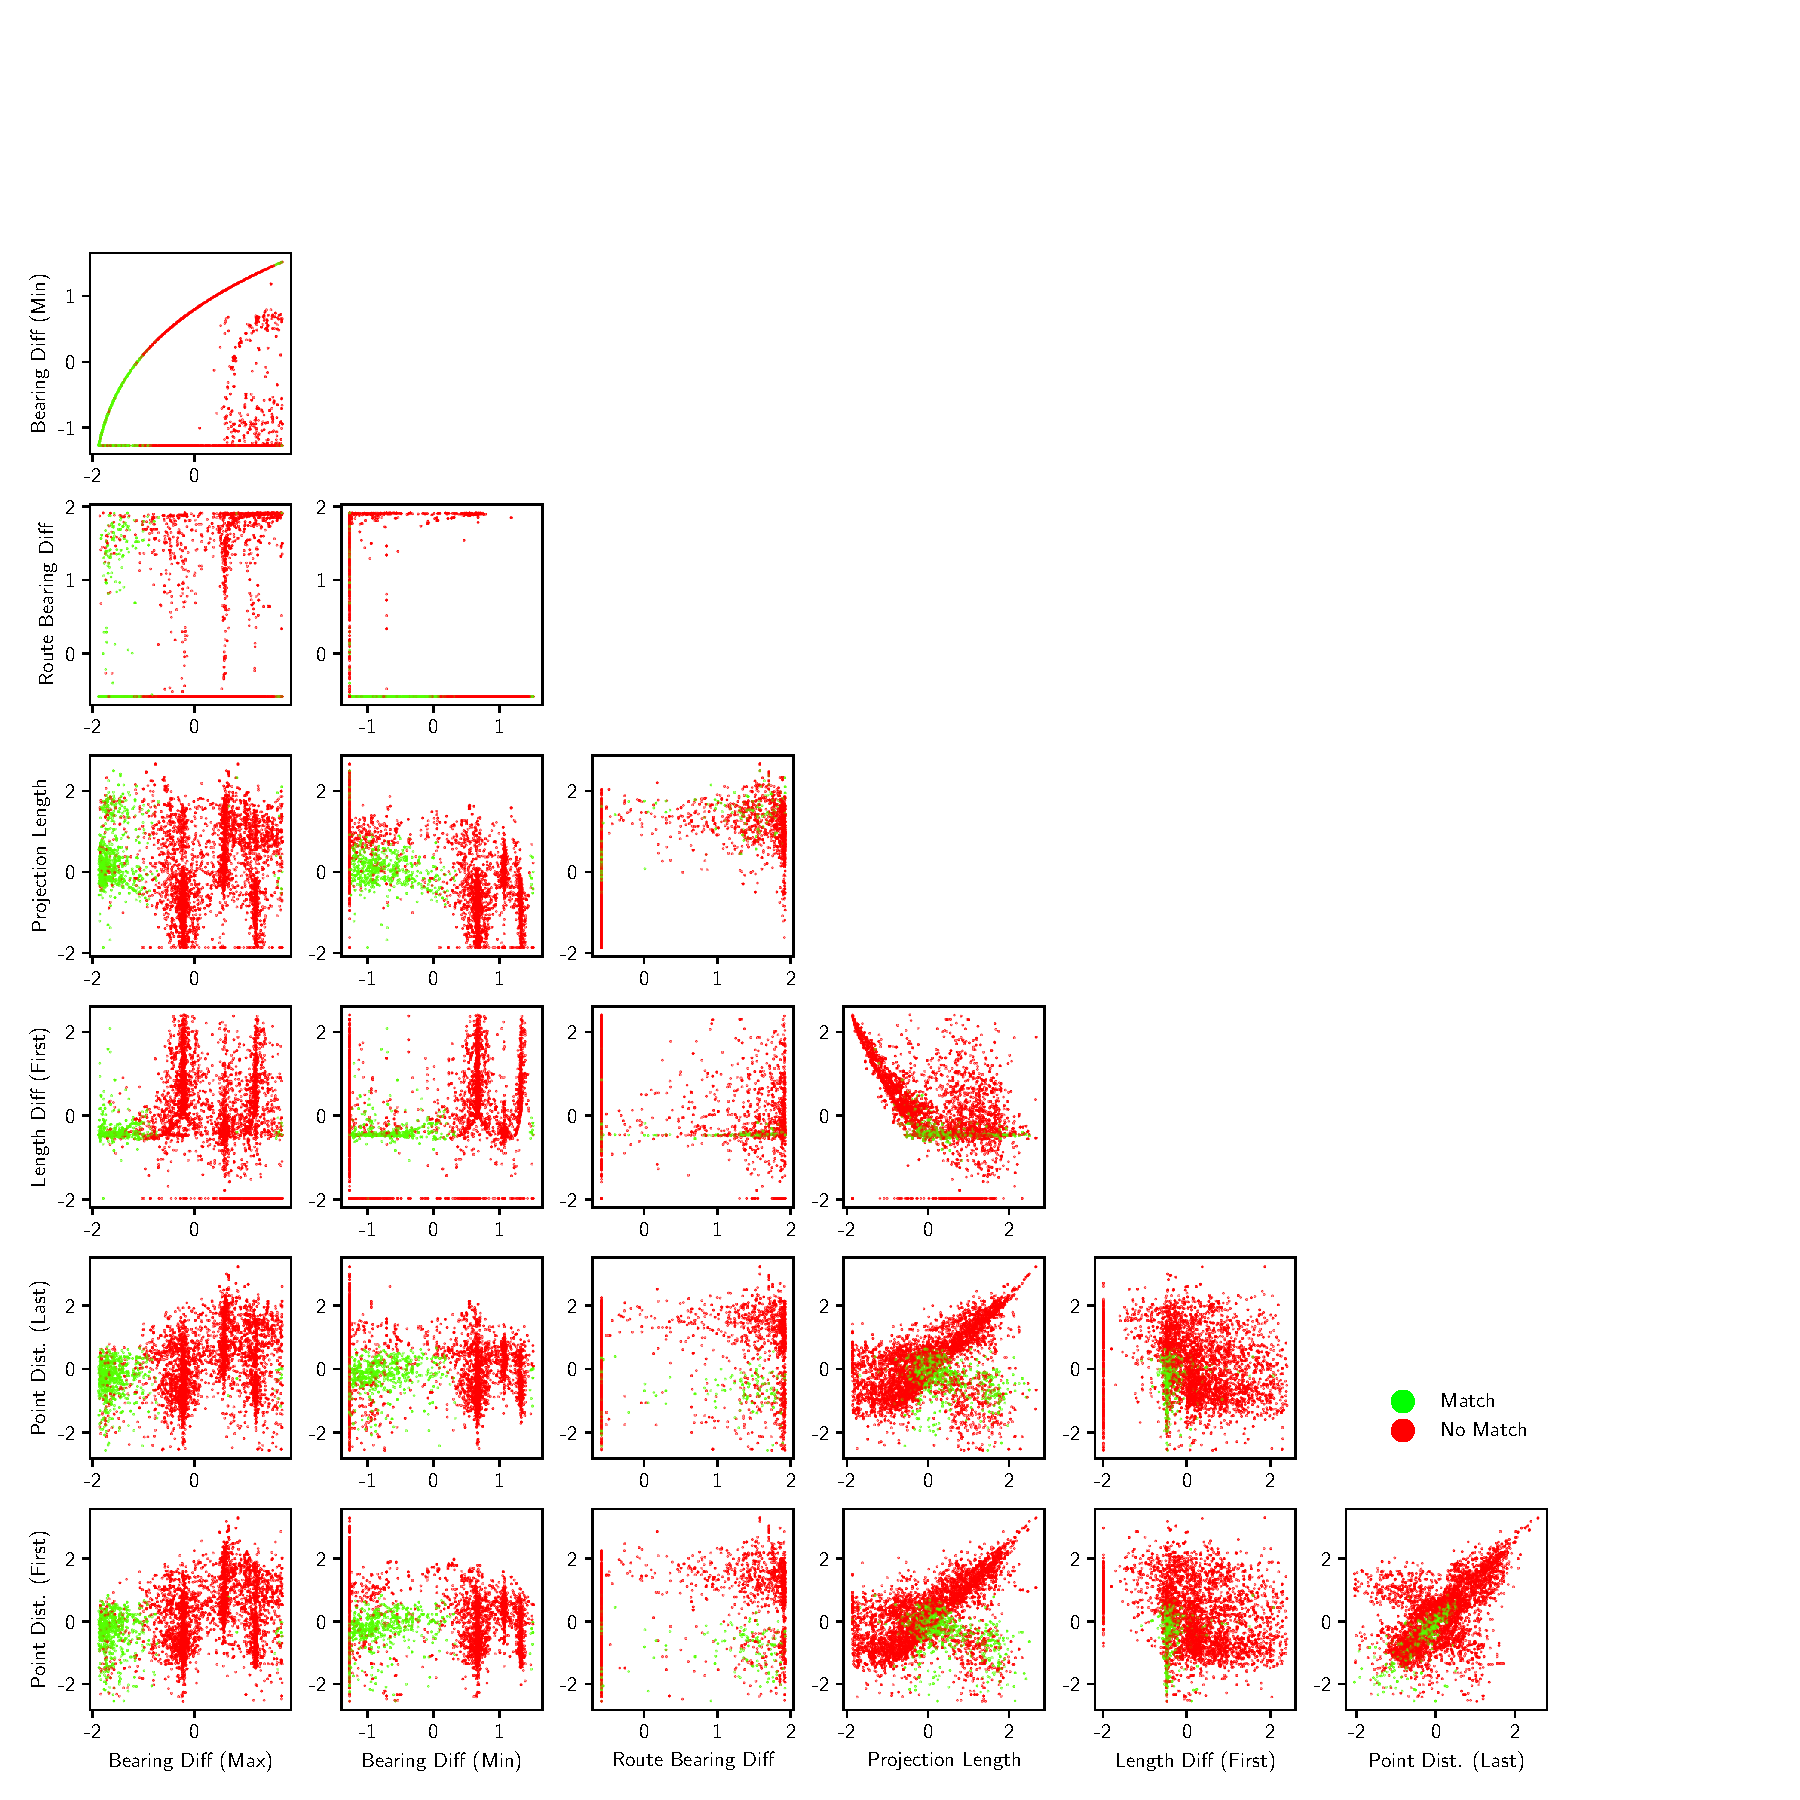
\includegraphics[width=\linewidth,bb=0 0 760 760]{images/decision-boundaries.pdf}
\caption{Decision boundaries of the ML model's Yeo-Johnson-transformed non-categorical features.}
\label{fig:ml-model-decision-boundaries}
\end{figure}

This relationship was successfully reconstructed by the hyperparameter model. Clear gradients are also noticeable at other thresholds. The loss gradients for the overlap thresholds T7 to T9 appear somewhat diffuse, aligning with the variability observed in these parameters in the final models. Overall, the hyperparameter tuning seems to have captured essential relationships effectively. At least, no better model could be manually found.

The ML model was trained on the 2022 OSM dataset and is evaluated on both OSM ground truths. The training and evaluation of the ML model are structured more complexly to effectively address overfitting issues via regularization. The analysis of the ground truth revealed increased redundancy, especially in the 2022 OSM dataset. Since this is also the dataset on which the ML model is trained, 3092 out of 6440 redundant examples were identified and removed based on matching feature vectors before training. The model training was conducted using Stratified K-Fold Cross-Validation over 342 epochs.

A look at the decision boundaries of the trained ML model allows us to gain a more precise understanding of its workwise. The gradual decision boundaries of the non-categorical features are shown in \Cref{fig:ml-model-decision-boundaries}. This visualization was created by inferring random routes on the model and recording the calculated features along with the predicted class. 

Since the input values have already been transformed into the feature space through the Yeo-Johnson transformation, the depicted relationships may not be evenly distributed across the input data. However, it is clearly visible, especially in the bearing features (max and min), that input values mapped to 0, which should lie around 180° opposite to the route, serve as exclusion criteria for non-matching lanes.

When the lane and the route are very close to each other (Point Dists), this is another strong indicator of a match. However, the observation that even near the zero line of Point Distances, where lanes presumably lie very close above the route, there are still many non-matching lanes is also interesting. As a consequence, the distance to the route does not seem to be a sole decision criterion, even for well-overlapping geometries. The same observation applies to the Length Diff feature.

Having explored the interpretability of the models, let's now focus on the achieved scores. These are presented in \Cref{tab:model-scores}.

\begin{table}[h]
\caption{Model evaluation scores.}
\begin{tabular}{@{}lllllllll@{}}
\toprule
  \textbf{Model} & \textbf{Benchmark} & \textbf{Trained on} & \textbf{TP} & \textbf{FP} & \textbf{FN} & \textbf{Precision} & \textbf{Recall} & \textbf{F1} \\
  \midrule
  Algorithmic & OSM 2022 & OSM 2022 & 920 & 207 & 123 & 82\% & 88\% & 84.8\% \\
  Algorithmic & OSM 2022 & OSM 2023 & 908 & 221 & 135 & 80\% & 87\% & 83.6\% \\
  ML          & OSM 2022 & OSM 2022 & 936 & 57 & 107 & 94\% & 90\% & 91.9\% \\
  \midrule
  Algorithmic & OSM 2023 & OSM 2022 & 615 & 159 & 143 & 79\% & 81\% & 80.3\% \\
  Algorithmic & OSM 2023 & OSM 2023 & 637 & 136 & 121 & 82\% & 84\% & 83.2\% \\
  ML          & OSM 2023 & OSM 2022 & 614 & 52 & 144 & 92\% & 81\% & 86.2\% \\
\bottomrule
\end{tabular}
\label{tab:model-scores}
\end{table}

The algorithmic model trained on the 2022 OSM dataset achieves an F1 score of 84.8\% on the same dataset, while the algorithmic model trained on the 2023 OSM dataset shows an F1 score of 83.6\%. These results suggest a robust performance of the algorithmic approach in validating on unknown data, even though a slight loss of accuracy is observed. Both algorithmic models generate relatively many false positives (FP) compared to the number of false negatives (FN), resulting in a low precision score of 82\% and 80\%, respectively.

The ML model trained on the 2022 OSM data effectively filters out false positives about four times more, yielding a precision score of 94\%. The recall is also slightly higher. Overall, the ML model achieves an F1 score of 91.9\% across the entire dataset, surpassing the comparable algorithmic model by 7.1\%. On the stratified k-fold cross-validation of the duplicate-corrected dataset, the ML model achieves a similar test score of 92\% (94\% training).

In the validation of the models on the 2023 OSM dataset, those trained on the 2022 OSM dataset perform less well. One possible explanation is that the 2023 OSM dataset contains significantly more connections that, together with the generated routes, represent new, unknown configurations for the model. The loss in the F1 score is mainly reflected in the lower recall, indicating that more traffic lights that actually belong to the route are being filtered out. Interestingly, even the algorithmic model optimized on the 2023 data performs worse on the 2023 OSM dataset than the model optimized on the larger 2022 OSM dataset. This suggests that a better result could have been achieved if the 2023 OSM dataset had been slightly larger.

Assessing how satisfactory these results are is challenging. Since the presented approach uses user-generated routes rather than real-time GNSS data, comparing it with location-based approaches is challenging. Assuming the user precisely follows the route would be questionable, given the inherent uncertainties in GNSS measurements and the imperfect representation of bike paths in the OSM route. Methodological uncertainties in implementing a location-based approach also hinder a meaningful comparison with other methods. The results from Koukoumidis et al. (2011–2012) \cite{koukoumidis_signalguru_2011, koukoumidis_leveraging_2012} cannot be directly compared, as they were calculated based on the number of correctly detected camera images rather than per traffic light. Therefore, an absolute interpretation of the results solely through comparison with other works is not possible, given the substantial differences in the fundamental ideas of the approaches.

Instead, what we can do is carefully examine areas where improvement potential exists and evaluate the approach's performance in real driving scenarios.

\begin{figure}[t]
\centering 
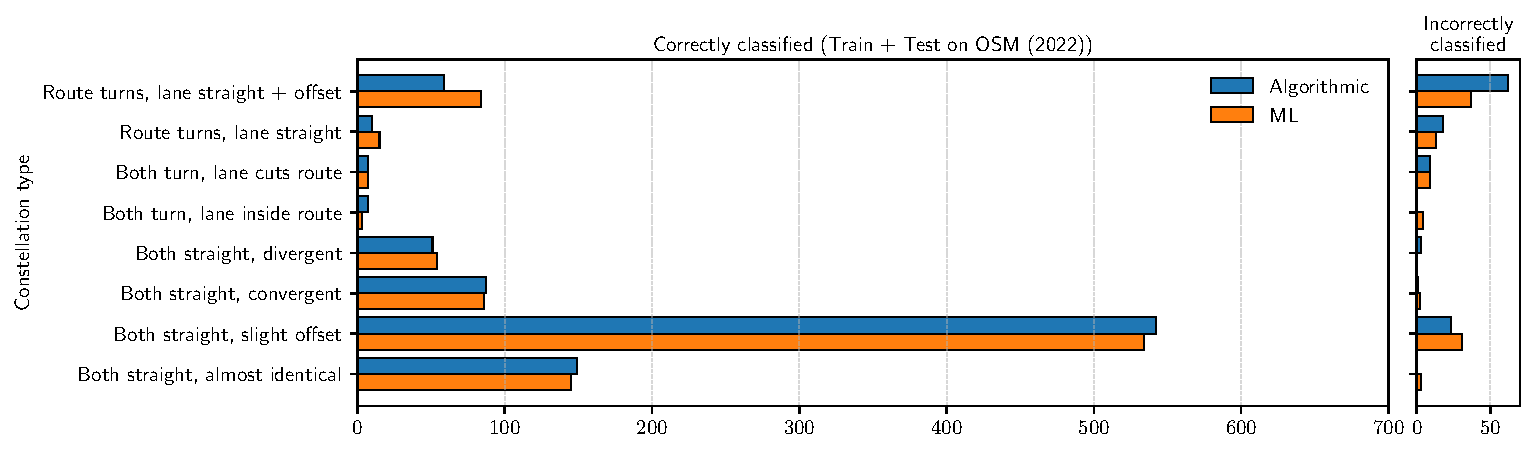
\includegraphics[width=\linewidth]{images/matching-constellations-osm-old.pdf}
\caption{Recorded types of constellation between route and traffic light geometry.}
\label{fig:matching-constellations-osm}
\end{figure}

\Cref{fig:matching-constellations-osm} examines the type of constellation between the route and traffic light geometry, which was specified during the creation process for the 2022 OSM ground truth for each selection. This could provide more detailed insights into the types of constellations where the models can be improved.

By far, the most common constellation is when the route and the lane go straight and are slightly offset from each other. With this constellation, the ML model seems to struggle slightly more than the algorithmic model. Even when both geometries almost exactly overlap and go straight, the ML model achieves a slightly lower score.

On the other hand, where the ML model performs significantly better is in situations where the route turns, but the corresponding lane goes straight and may also have an offset from the route. This occurs, for example, when the route turns left over the car lanes at an intersection, but a short straight bicycle signal to the right needs to be selected.

These situations occur more frequently than expected and are closely related to the imprecise bicycle routing in OSM.

\begin{figure}[t]
\centering 
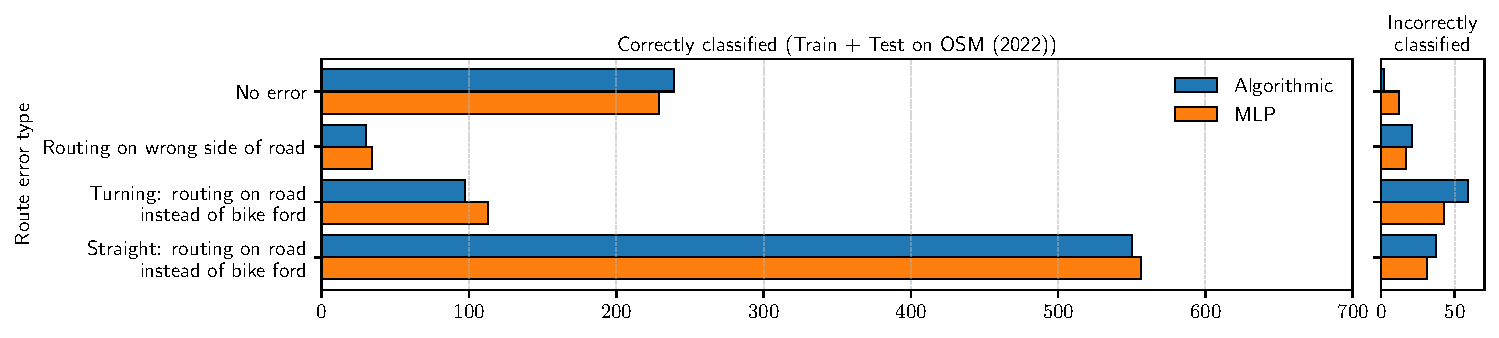
\includegraphics[width=\linewidth]{images/matching-route-errors-osm-old.pdf}
\caption{Recorded types of routing errors annotated to each constellation between traffic light and route.}
\label{fig:matching-routing-errors-osm}
\end{figure}

The analysis of route-lane constellations (\Cref{fig:matching-routing-errors-osm}) reveals that only a relatively small number of route-lane constellations exhibit no routing errors. This assessment involved marking both the constellation type in the Route Composer and any occurring routing errors. In the majority of cases, approximately 72\%, the route does not utilize the bicycle lane or bicycle ford at traffic lights but instead follows the center of the road. This occurrence is more than twice as frequent as instances with no routing errors.

In some cases, routing occurs on the wrong side of the street. The ML model demonstrates a higher accuracy of 86\% in detecting routing errors and correctly associating them with the traffic light geometry, surpassing the algorithmic model's 78\% accuracy. When no routing errors are present, the algorithmic model marginally outperforms the ML model with an accuracy of 96.2\% compared to 95.15\%. However, this advantage diminishes significantly in the presence of routing errors associated with OSM.

The ML model proves superior in matching traffic lights compared to the algorithmic model, leading to its selection as the final model for OSM matching provided to app users. The remaining concerns revolve around evaluating real-world application performance and scalability over longer routes or additional traffic light geometries.

Further insights into user perception of the matching process will be explored in \Cref{ch:impacts} through user surveys. Meanwhile, our focus here is on quantitative validation in real-world scenarios. Initial considerations involving the use of user tracks for validation were dismissed due to significant GNSS trajectory drift, making it challenging to identify which traffic light was utilized.

An alternative validation method was adopted. On March 21, 2023, four test rides with good prognosis availability were conducted and filmed using a camera. The app calculated routes for these rides, and the final version of the matching algorithm automatically selected traffic lights. Subsequent video analysis confirmed the correct selection of 51 out of 56 passed traffic lights, resulting in an accuracy of 91.07\%. These measured results align with the ground truths, validating the effectiveness of the matching algorithm.

\begin{figure}[t]
\centering 
\includegraphics[width=\linewidth]{images/matching-performance-556-routes.pdf}
\caption{Relation between number of traffic lights, route length, and matching time measured on the Beta deployment.}
\label{fig:matching-performance}
\end{figure}

Finally, we examine the response time of the final service using the ML matching method. This metric is crucial as users do not want to wait indefinitely for route calculation and matching. Even in the case of automatic route recalculation, the functionality of speed recommendation should be restored quickly.

In \Cref{fig:matching-performance}, a measurement is presented based on 556 random routes on the Beta deployment at TU Dresden. The load is distributed using the round-robin method across four individual containers with the matching service, each located on an enterprise VM at TU Dresden. The measured time is deployment-dependent and also influenced by the host system/network from which the measurement is taken. However, the exact number of milliseconds is not as crucial as the order of magnitude and its correlation with route length and the number of traffic lights along the route.

The median matching time is 1.4 seconds, with the 75th percentile at 2.1 seconds. Users can expect approximately this time for both route calculation and traffic light selection. While optimization, for example, through implementation in a faster programming language than Python, is not urgently necessary, it should be considered as a potential improvement. The observed matching time is generally satisfactory in the current state.

It is evident that the matching time correlates with the route's length. The more traffic lights along the route, the longer the process tends to take. This is expected since the ML model likely needs to search through more intersections, not filtered out by the initial, very efficient distance filter around the route.

However, there are also longer routes that are matched relatively quickly due to a lower number of connected intersections. Routes longer than about 50 km were not generated, as traffic lights are only available in the Hamburg area. This consideration is important if the method is to be applied on an inter-city level with significantly longer routes and many more intersections.

\begin{Summary}[Summary and Discussion of Results]
While the challenges of a location-based approach have already been described in related work, the results also speak against such an approach. The cyclist's planned trajectory over the upcoming intersection must be known in order to accurately determine the appropriate traffic lights and give the user enough reaction time to the speed advisory. Two ground truths with human-made choices for the best traffic light were created. The analysis of these ground truths indicates that many traffic lights theoretically available for bike usage are never chosen as appropriate matches, especially in the presence of dedicated bike traffic lights. As a consequence, newly labeled routes quickly do not introduce new examples anymore, limiting the overall ground truth size. 

Trained on the ground truths, the angular relationship between traffic light geometries and the route seems to be an especially important decision criterion between "match" and "no match." While the 2022 algorithmic model achieves an F1 score of 84.8\% on the 2022 dataset, its score drops to 80.3\% when validated on the 2023 dataset, containing double as many traffic light geometries. The 2022 ML model achieves a much higher test F1 score of 92\% during k-fold cross-validation and also drops to 86.2\% validated on the 2023 dataset. 

Only a few false matchings are made when the traffic light geometry and the route closely overlap. The biggest potential for improvement resides in routing on the road instead of the bike infrastructure, which is more than two times as prevalent as cases without routing errors. Although the models are able to compensate for this issue to some extent, the results suggest that an improved routing could significantly boost the matching performance. Finally, it is shown that the matching can be executed in a time frame of less than two seconds in most cases, with routes of up to 50 km. 
\end{Summary}

\section{Conclusions}

Accurate and timely traffic light matching is crucial for an effective speed advisory. Nonetheless, how to achieve such a matching has not received much research attention. While vision-based methods are highly advanced, their practicality for handlebar-mounted smartphones is limited. Matching the cyclist's real-time position to nearby traffic light geometries is also not an option due to the ambiguity and shortness of these geometries, as well as GNSS inaccuracies. Anticipating turns through a bike route and looking up nearby traffic lights is a better option. However, this lookup is not trivial since calculated bike routes do not align with the suitable traffic lights. In many cases, traffic lights are offset to the route but still a good match.

In this chapter, we developed two methods that enable accurate traffic light matching even in the presence of imprecise and erroneous OSM bike routes. The algorithmic model and the ML model utilize geometric relationships between each traffic light geometry and the corresponding route to filter out suitable matches. The ML model achieves a test F1 score of 92\% on a 2022 ground truth and an 86.2\% F1 score on a separate validation ground truth from 2023. A matching is achieved on arbitrary OSM bike routes through Hamburg in approximately 1.4 seconds, allowing users of the app to freely, accurately, and quickly choose any route through the city. Bike traffic lights are preferred whenever possible. The developed approach has the advantage that it should work with practically any city and does not exhibit noticeable difficulties with short traffic light geometries. Its only requirement is the availability of traffic light geometries, which are expected to be relatively widespread in the form of MAP geometries due to the global expansion of C-ITS services.

However, the developed approach also has limitations that open up new opportunities for future work. An alternative solution to the proposed matching algorithms could be arriving at a georeferenced bicycle network graph that contains all traffic light IDs. Such a network graph is currently not available for Hamburg \cite{neuner_leitfaden_2020} but could be theoretically developed in the future. One potential source for a more accurate path network -- proprietary HD maps -- could not be investigated due to limited accessibility. Currently, these maps are primarily intended for cars and are likely not a good solution to generate bike routes. Ideally, it would even be possible to automatically generate such a network graph for cycle paths using publicly available data. Learning how to put this idea into practice, and whether this is possible at all, would also be a potential subject for future work. Until such a solution is viable, one potential improvement for the presented approach is decreasing the routing errors as much as possible and improving the overall alignment of bike routes with the traffic light geometries. This challenge and its influences on matching accuracy will be investigated in the following chapter.
  \chapter{Accurate Bike Routing}\label{ch:routing}

\begin{Summary}[Bibliographical Notes]
This chapter is based on the following paper in which the author was the principal investigator:

\cite{matthes2023accurate} \fullcite{matthes2023accurate}
\end{Summary}

\section{Introduction}

The mobility behavior in urban environments is becoming increasingly intermodal. The trend is moving towards a multimodal mobility planning \cite{park_framework_2023}, where bike-sharing and bike routes also play a significant role. Understanding cyclists' behaviors, particularly their route choices, is crucial not only for calculating preferences for suitable cycling routes but also as a fundamental aspect of expanding cycling infrastructure and urban planning \cite{zielstra_comparative_2011, huber_modelling_2021}. Models that replicate cyclists' route choices provide immediate insights into where cycling infrastructure should receive high priority. Effective route selection is indispensable for bicycle navigation applications, but the challenge lies in the high individuality and context dependence of chosen paths \cite{dill_revisiting_2016, schleinitz_german_2017, misra_modeling_2018}, resulting in a multi-criteria optimization problem \cite{song_exploring_2014}. Route choices depend not only on road conditions but also on factors such as bicycle type and personal preferences, making it challenging to compute optimal routes for cyclists.

In the context of GLOSA applications, routing is linked to additional factors. It is essential not only for the cycling route to follow reasonable paths but also to accurately align with bicycle lanes for precise traffic light matching. The closer the route aligns with the bicycle lane, the better it serves distance estimation to the traffic light. Accounting for bends or obstacles on the way to the traffic light ensures accurate distance estimation, preventing the speed recommendation from deviating from the actual speed. Additionally, factors such as route incline and road conditions contribute not only to routing but also serve as crucial information sources for speed recommendations. Accurate and consistent meta-information is desirable in these cases and must be obtained from a routing foundation.

Commercial map providers provide highly accurate map material but currently have the drawback of limited openness and extensibility. Considerations about copyright, privacy, costs, and vendor lock-ins are also relevant for these map providers, rendering them unattractive for many services. Thus, OpenStreetMap has established itself as the most popular foundation for various acknowledged solutions, such as Openrouteservice\footnote{\url{https://openrouteservice.org/}}, Photon and Komoot\footnote{\url{https://photon.komoot.io/}}, and Mapbox\footnote{\url{https://wiki.openstreetmap.org/wiki/Mapbox}}. Apple Maps and Bing Maps also use OpenStreetMap wherever no commercial data providers are available\footnote{\url{https://wiki.openstreetmap.org/wiki/Apple}, \url{https://wiki.openstreetmap.org/wiki/Bing_Maps}}. 

Despite being a highly recognized map foundation, an ongoing issue is that OpenStreetMap's accuracy and consistency vary due to its Volunteered Geographical Information (VGI) concept \cite{wasserman_evaluating_2019, jacobs_openstreetmap_2020, vybornova_automated_2023}. As a result, bicycle routes generated with OpenStreetMap may not always achieve the desired accuracy. With a highly engaged user base and various company-level contributors, OpenStreetMap profits from frequent updates. However, similar to Wikipedia, not all contributions are of high quality. As a result, bike paths are not always captured as separate geometries from the road or tagged with the correct properties.

In this chapter, we introduce an open alternative for accurate bicycle routing. We propose methods to reuse bike infrastructure reference models (authoritative datasets) that are institutionally maintained and released under open-source licenses. An example is the "Digitales Radnetz Hamburg" (Digital Cycling Network Hamburg, DRN), specifically designed for cycling paths in Hamburg. Such models promise a significantly more accurate and consistent resolution of cycling paths, making them an attractive solution for a GLOSA app. Other municipalities provide such models as well \cite{englede_efficient_2013, brovelli_towards_2017}. 

However, infrastructure reference models face the challenge of lacking global coverage. In the case of DRN, it covers only the city of Hamburg, making routing across city borders challenging. Solutions need to be devised for integrating the dataset with routing profiles for cyclists, addressing various technical challenges. Given that both DRN and OpenStreetMap lack elevation data, selecting the best provider from several available elevation providers is crucial. The goal is to outline precise steps that can help utilize similar datasets for bicycle routing in other regions and develop an open routing engine applicable beyond the GLOSA app for accurate bicycle routing in Hamburg.

Apart from the methodological aspect, the core contribution primarily lies in the results section. A key focus is evaluating how much the accuracy of traffic light matching can be improved with a potentially more precise representation of cycling paths, compared to results from \Cref{ch:matching}. The primary contribution is determining the effectiveness of routing based on this type of dataset by comparing alignment with cycling infrastructure and the number of routing errors. Ideally, using the open DRN routing foundation should resolve many of the issues found with OpenStreetMap bike routing, providing users of the bike-GLOSA app with much better directions and speed recommendations.

\section{Related Work}\label{sec:rw-uis}

Establishing an accurate bike routing is a multifaceted research area. One avenue of investigation focuses on models that can predict cyclists' route choices with high accuracy based on available metadata \cite{dill_understanding_2008, ghanayim_modelling_2018, huber_modelling_2021}. This involves correlating GNSS trajectories with routing networks to understand the relationships between path characteristics and route selection \cite{sultan_extracting_2017, huber_modelling_2021}. Some studies also focus on safe bike routing \cite{loidl_online_2018}, popularity-based routing \cite{bergman_conflation_2016} or the short-term effects of infrastructure changes on cyclists' route preferences \cite{yeboah_route_2015, pritchard_does_2019}. Over the years, open routing engines such as GraphHopper\footnote{\url{https://www.graphhopper.com/}} have continuously improved, providing community and research-tested routing profiles tailored for various types of cycling. Thus, although there are optimization opportunities for bike routing profiles \cite{krismer_elevation_2016}, the available ones can be considered well consolidated.

Our focus will be on the issue of achieving a more accurate routing foundation and its application scenarios in GLOSA systems. First, we will discuss the status quo of bike path consistency and accuracy in routing foundations. Looking for solutions to the problem, we will investigate methods that utilize external authoritative datasets to improve the overall quality and alignment of bike path segments. Subsequently, we will delve into several challenges for GLOSA systems where precise routing emerges as a key solution. These challenges include multi-segment GLOSA, GNSS error correction, context-sensitive speed advisories, traffic light matching, and distance-to-signal estimation.

\subsection{Bike Path Consistency and Accuracy in Routing Foundations}

How accurately and consistently a bike routing can be performed depends on the specific kind of routing foundation.

None of the competitors Google Maps, Bing Maps, and OpenStreetMap, excels in a consistent and accurate depiction of bike paths. Ciepluch's comparison in 2010 \cite{ciepluch_comparison_2010} revealed that Google Maps, Bing Maps, and OpenStreetMap did not significantly differ in quality, with no platform emerging as a clear winner. Similarly, a more recent study by Franzini et al. (2020) \cite{franzini_assessment_2020} found that only 40\% of the Pavia region in Italy is fully mapped in OpenStreetMap and 30\% in Google Maps, based on 2018 data. These findings emphasize the incomplete coverage of both platforms, though this study is not specifically focused on bicycle paths.

Hochmair et al. (2015) \cite{hochmair_assessing_2015}  specifically assessed the coverage of bicycle infrastructure, noting variations in completeness. In Portland, 86.4\% of 26 km of bicycle trails were correctly captured in OpenStreetMap, compared to 78.4\% in Google Maps. However, in Miami, only 22.8\% (OpenStreetMap) and 36.5\% (Google Maps) of 22 km of reference paths were accurately recorded, with a significant omission of paths along recreational sites such as rivers and parks. Additionally, Ferster et al. (2019) \cite{ferster_using_2019} and Wasserman et al. (2019) \cite{wasserman_evaluating_2019} highlighted inconsistencies in meta-information about bike path quality in OpenStreetMap, impacting the determination of bikeability. Vybornova et al. (2023) \cite{vybornova_automated_2023} demonstrated that connectivity issues in bicycle path segments could disrupt meaningful route calculations, collectively indicating deficiencies in the coverage of bicycle infrastructure by OpenStreetMap and alternatives like Google Maps.

Identifying errors in OpenStreetMap data is relatively well investigated. Authoritative datasets have been used as ground truths for comparison, as demonstrated by various studies \cite{haklay_how_2010, jokar_arsanjani_quality_2015, ludwig_comparison_2011}. Brovelli et al. (2017) \cite{brovelli_towards_2017} introduced a framework for comparing open reference map data with OpenStreetMap for enhanced reusability. 

However, the question remains how the detected issues can be systematically resolved. Vybornova et al. (2023) \cite{vybornova_automated_2023} recently suggested a method to detect and rectify missing connections between bike paths, though this approach does not address missing meta-information or entirely absent bike paths. Nasiri et al. (2018) \cite{nasiri_improving_2018} introduced a multi-stage approach in which outliers are detected in OpenStreetMap histories, improving the positional precision of features by 14\% in Teheran.  

Some studies explore connecting meta-information from a reference model to OpenStreetMap for a more consistent metadata coverage, utilizing map-matching directly or methods that resemble established map-matching approaches \cite{chao_survey_2020}. Szwoch (2018) \cite{szwoch_combining_2019} demonstrated the integration of OpenStreetMap routes with metadata from an authoritative database. Fan et al. (2016) \cite{fan_polygon-based_2016} also examined this approach. Meister et al. (2023) \cite{meister_route_2023} studied cyclists' route choices in Zurich, using map-matching to incorporate metadata from a municipal dataset due to OpenStreetMap's insufficient consistency. All three approaches address the issue of inconsistent metadata but not the issue of inaccurate route geometries as a result of missing or imprecise routing network geometries.

Building on these ideas, Smarzaro et al. (2021) \cite{smarzaro_creation_2021} demonstrated how data from multiple authoritative datasets and Volunteered Geographic Information (VGI) can be fused for improved multimodal routing. The focus is on uncovering unknown paths, such as footpaths in parks or parking lots, and associated meta-information. The authors propose a method where each GeoFeature from an external dataset is compared to nearby paths, and if new, it is added to the dataset. However, the challenge lies in defining suitable thresholds to distinguish overlapping from non-overlapping segments. The study, unfortunately, only compares travel distances with Google Maps without a thorough assessment of improved coverage or accuracy. Whether bike paths are captured separately to nearby segments and, thus, how the resolution of intersection topologies is affected is also unclear.

Li et al. (2017) \cite{li_optimized_2017} demonstrate how OpenStreetMap can be inserted into an authoritative bikeway dataset to enhance the overall accuracy of bikeway geometries and metadata. The authors employ a semi-automated approach with a human-in-the-loop that performs four steps: first, the datasets are preprocessed to ensure their consistency and correct geographical projection. Afterward, the datasets are automatically conflated, including metadata mapping to match OpenStreetMap path tags to four path categories in their authoritative dataset. In the third and fourth steps, the quality of paths is evaluated using the feature matching uncertainty and a human eye, allowing a human to manually adjust false matchings. In their evaluation, the authors found their system to achieve a relatively high precision of 92.54\%. 

Here, it needs to be considered that the authors conducted their study on a relatively sparse bike path dataset in Los Angeles. Thus, one main limitation the authors noted is the reliance on a human. A fully automated approach would be desirable to account for the continuously evolving bike infrastructure without having to conduct a manual correction process on a daily basis. Furthermore, the authors claim to have improved positional accuracy of the bike path geometries. However, no concrete measures w.r.t to a ground truth are presented. Further investigations are required to address these limitations.

\subsection{Application Scenarios of Routing in GLOSA}

- Multi-segment GLOSA
- GNSS Error Correction
- Metadaten für Kontextsensitivität und Routing-Profile
- Traffic light matching
- Distance-to-signal estimation

\section{Concept}

\subsection{DRN Routing}

Routing with GraphHopper and OpenStreetMap has the advantages of worldwide support and frequent updates of the community. However, the quality and consistency of the map materials vary from location to location. Since OpenStreetMap is a general-purpose map foundation, bike paths are often not represented as separate geometries but instead merged with the nearby road. This leads to the problem that some roads have separate bike path geometries running alongside, and others don't. Hence, when calculating a bike route based on OpenStreetMap, the bike route often jumps on or off the road. This degrades the distance-to-signal estimation, traffic light matching, and overall in-app routing. Although the system may work with OpenStreetMap, this situation is still not ideal.

To counteract this problem, it is vital to look for other routing foundations than OpenStreetMap that model the bike paths more accurately. As a solution, the dataset "Digitales Radverkehrsnetz Hamburg"\footnote{\url{https://metaver.de/trefferanzeige?docuuid=EA847D9F-6403-4B75-BCDB-73F831F960C7}} (DRN) has been identified. The dataset is institutionally maintained and contains all bikeable paths in Hamburg. Based on preliminary comparisons with OpenStreetMap, the DRN dataset promises a more consistent and quality-assured depiction of bike paths.

\begin{figure}[htbp]
\centering
\begin{subfigure}
  \centering
  \includegraphics[width=\linewidth]{images/legend-fig-1.png}
\end{subfigure}
\begin{subfigure}
  \centering
  \includegraphics[width=.49\linewidth]{images/osm-route.png}
\end{subfigure}%
\begin{subfigure}
  \centering
  \includegraphics[width=.49\linewidth]{images/drn-route.png}
\end{subfigure}
\caption{Alignment of OpenStreetMap vs. DRN with the intersection topology. Image source: [in print].}
\label{fig:comparison}%
\end{figure}

\Cref{fig:comparison} shows a specific example of OpenStreetMap routing on the road when no separate bike path geometry is captured. With DRN the bike path is not only captured as a separate geometry but also aligns more closely with the bike path's curvature. Thus, the speed advisory could also be more precise as the signal's distance may be estimated more accurately. \Cref{fig:comparison} also highlights that the DRN route may align more closely with the bike signal's geometry, while the OpenStreetMap route is closer to the car lanes. Assuming that a cyclist follows the designated bike path, less speculation is required as to which traffic light must be matched. 

Due to these prospects, a system was created that allows for DRN-based bike routing inside Hamburg and OpenStreetMap-based bike routing outside Hamburg. To make DRN ready for routing, several processing steps were established as part of a publication at ITSC 2023 [in print], based on the supervised Diploma thesis of Max Lorenz (2022) \cite{lorenz_2022}: First, the DRN format must be translated into a data format that a routing engine understands. Then, the map's topology must be optimized such that routing errors are minimized. Finally, OpenStreetMap and DRN must be merged together at the city's border to allow a seamless transition.

\subsubsection{Translation from DRN to OpenStreetMap}

\begin{figure}[htbp]
\centering
\includegraphics[width=\linewidth]{images/drn-map.png}
\caption{An overview of the DRN dataset and its top-10 bike path types.}
\label{fig:drn-map}
\end{figure}

The DRN dataset can be downloaded in various geodata formats such as CSV, GeoJSON, or GML. Each contained data point refers to a path segment and is associated with metadata tags. Among others, the following properties are mapped\footnote{The displayed statistics represent a snapshot of the 23rd of August 2023.}:

\begin{itemize}
    \item Direction of travel (49852 segments bidirectional and 47692 segments unidirectional)
    \item Time restrictions (32 segments affected)
    \item Temporary paths such as pop-up lanes or detours (83 segments affected)
    \item If a segment is associated with a specific velo route or designated bike tours (Freizeitroute)
    \item Level (96237 flat, 1121 across bridges, 186 through tunnels)
    \item Obstacles (456 impassable, 52 can be circumvented e.g. via footpath)
    \item The type of bike path and its surface
    \item Target and end node ID of the segment connecting the segments to a graph
    \item The segment's coordinates
\end{itemize}

Now, to calculate routes based on the dataset, it is necessary to make the dataset available to the routing engine. Here, it is possible to design a plugin for the routing engine that allows it to read the dataset's format. However, a better solution is to transform the DRN dataset into the OpenStreetMap format. In this way, the existing routing engine and its community-tested routing profiles can be reused without modifying the engine's internals. Furthermore, transforming the DRN dataset to OpenStreetMap simplifies merging both datasets together at the city border. Thus, a map transformer was designed in [in print] that converts the DRN format to OpenStreetMap.

The routing profiles utilize weights of the properties annotated to each OpenStreetMap path to calculate a personalized route. The challenge here is that DRN specifies other properties than OpenStreetMap. For example, DRN specifies three types for compacted surface: "befestigt - nicht genauer erkennbar", "befestigt - zu detailieren" and "Wassergebundene Decke". To resolve this problem, a mapping was developed that infers the OpenStreetMap tags from the DRN specification. This mapping includes the bike path's surface, level, direction, and type (as shown in \Cref{fig:drn-map}). In cases where the bike path's properties cannot be directly mapped to a suitable OpenStreetMap tag, the path is tagged with \texttt{highway = tertiary}. As noted in [in print], this follows established mapping practices in Germany. The result is an inferred set of tags for each path in the OpenStreetMap format.

\subsubsection{Error Correction Methods}

After the map conversion into the OpenStreetMap format, there are still some problems with the map material that must be addressed. In [in print] two problems were identified when generating routes with the converted DRN network: detours resulting from duplicated nodes in the graph and detours because the road cannot be crossed.

\begin{figure}[htbp]
\centering
\includegraphics[width=\linewidth]{images/node-merging.png}
\caption{Duplicated nodes (left) are merged together (right) to avoid detours. Source: [in print]}
\label{fig:node-merging}
\end{figure}

\paragraph{Duplicated nodes:} Each individual path in the DRN dataset starts and ends in a node, which must be transformed into OpenStreetMap nodes that connect the individual paths to a graph structure\footnote{\url{https://wiki.openstreetmap.org/wiki/Node}}. To ease this process the DRN dataset provides node IDs for the start and end point of each path. Thus, two nodes are generated for each path based on the start and end coordinates given in the line geometry. Since there may be multiple paths that are connected to a node, the same node is generated multiple times during dataset processing. In theory, this is not a problem since the node ID can be utilized to avoid duplicates. In practice, however, sometimes there are nodes for which multiple different coordinates are found in the dataset. Due to presumably floating point or geographic projection inaccuracies in the dataset, the coordinates may be misaligned by a few centimeters.

As discussed in [in print], the developed solution involves calculating a center point for each node ID. Let $C_k = \{c_{k_1} = (lat_{k_1}, lng_{k_1}), \text{...} , c_{k_n} = (lat_{k_n}, lng_{k_n})\}$ be the collected coordinates for each node $k$. Then, the center point $\text{Center}_{\text{k}}$ is calculated as $\text{Center}_{\text{k}} = \left(n^{-1} * {\sum_{i=1}^{n} \text{{lat}}_{k_i}}, {n^{-1} * \sum_{i=1}^{n} \text{{lng}}_{k_i}}\right)$. The resulting coordinates are utilized to connect the generated paths. To validate this approach, the maximum relocation distance between all $\text{Center}_{\text{k}}$ and $c \in C_k$ was calculated as 8.3 centimeters using the haversine formula. Based on this result, no further points were falsely connected.

\paragraph{Non-crossable roads}: Since bike paths on both roadsides are captured as individual geometries in the DRN dataset, there may be long road segments with bike paths running in parallel. However, without interconnections between the roadsides, there is also no possibility for the route to cross the road. Sometimes, this represents a problem since side roads attached to the opposite roadside can only be reached by long detours. With OpenStreetMap, this is a lesser problem since roads are often captured as single-path geometries without a clear distinction between each roadside. 


\begin{figure}[htbp]
\centering
\includegraphics[width=\linewidth]{images/oneway-travel-fix.png}
\caption{Detour (left) that can be fixed by enabling opposite-direction one-way travel on foot (right), compared to OpenStreetMap route (blue). Source: [in print]}
\label{fig:oneway-travel-fix}
\end{figure}

One solution explored in [in print] is the introduction of "virtual" paths connecting the roadsides. Using these paths, the route could traverse between roadsides and avoid detours. Although this concept may sound like a reasonable idea at first, the question is where to place these virtual paths. For example, one could place these paths in a fixed interval along a road between roadsides. However, there could always be a physical barrier between both roadsides, meaning that generated routes would guide users over impassable obstacles or potentially encourage dangerous maneuvers. Traversing a road at an arbitrary location may not always be safe or legal. Due to these reasons, the idea of inserting virtual paths was discarded.

As discussed in [in print], the final solution takes another approach. In the DRN dataset, bike paths are marked for travel in one direction or two directions. Here, the error source for detours is often the restricted one-way travel direction along the bike path. In cases where detours are observed due to long paths down the street until the next road crossing, it is likely that a similar road crossing lies closer up the street. Thus, a solution is to allow opposite-direction one-way travel on foot. This solution assumes that the bike can safely and legally be dismounted and walked in the opposite direction.

\subsubsection{Routing Outside of Hamburg}

The DRN dataset's coverage ends at Hamburg's city border. This means that, although the dataset provides full coverage within the region of Hamburg, the dataset must be combined with another map foundation to provide routing outside the city. Here, it is possible to fall back to the OpenStreetMap dataset. However, the geometries of both datasets don't align. To provide continuous routing over the city border, both datasets must be stitched together. 

The conflation process presented in [in print] starts with matching the OpenStreetMap paths to the associated DRN paths along the city border. First, DRN nodes close (<20m) to the border are fetched. For each of these DRN nodes, the 5 nearest OpenStreetMap paths are treated as a possible match. However, the OpenStreetMap paths may traverse the city border without a node lying exactly on the border geometry, potentially leading to z-shaped connections between OpenStreetMap and DRN. To avoid this problem, the conflation process inserts artificial OpenStreetMap nodes at the intersection of the city border geometry. Finally, for each DRN node, the nearest (interpolated) OpenStreetMap node is selected and connected. As a result, the DRN paths are stitched to the OpenStreetMap paths along the city border.

Finally, the error-corrected and stitched path network is exported in the OpenStreetMap format. The exported map data is integrated with GraphHopper and replaces the original OpenStreetMap-only GraphHopper routing engine utilized by the mobile application.

\subsection{Digital Elevation Model}

With the chosen concept, users can personalize the routing algorithm to avoid inclines. In Hamburg, this may be less of a concern, but there are still several roads with non-negligible inclines such as Helgoländer Allee. However, DRN and OpenStreetMap don't directly include height data of the road network. Thus, without an external digital elevation model, the routing engine cannot consider paths accordingly using the specified routing profile. Fortunately, GraphHopper has a built-in option for integrating a digital elevation model.

As briefly discussed in [in print], there are multiple digital elevation models that can be used. By default, GraphHopper supports SRTM (Shuttle Radar Topography Mission) \cite{farr_shuttle_2000, farr_shuttle_2007} and CGIAR \cite{jarvis_hole_2008} height data. The CGIAR height data is a proprietary post-processed version of the SRTM data, filling in data gaps in the SRTM height map, and is available under license to all GraphHopper users. By default, the routing engine is specified to use the SRTM dataset.

SRTM-1 offers a horizontal resolution of approximately 30m (1 arcsecond). For specific areas, additional SRTM X-SAR 25m data is provided by the DLR. For the covered regions of the SRTM X-SAR 25m model, the vertical precision is specified at $\pm$ 6m (relative vertical error at 90\% confidence level)\footnote{SRTM X-SAR 25m specification: \url{https://geoservice.dlr.de/web/dataguide/srtm/}}. An even higher precision is offered by the DGM-1 model for Hamburg in which the 1 stands for 1 meter of horizontal resolution. In this model, the vertical resolution is specified as $\pm$ 15cm\footnote{\url{https://metaver.de/trefferanzeige?docuuid=A39B4E86-15E2-4BF7-BA82-66F9913D5640}}. The high precision is reached by airborne laser scanning. Downscaled resolutions are available as DGM-10 (10m) and DGM-25 (25m).

To evaluate if the DGM models provide an overall better height profile than SRTM, Max Lorenz analyzed cross-sections of the height models. Another important question of this work was how much resources the model consumes when loaded into the routing engine. The results, which have briefly been referenced in [in print], show that the best tradeoff between resource usage and model accuracy is provided by the DGM-10 model. Thus, the DGM-10 model was integrated as the final digital elevation model into the GraphHopper routing engine using a custom tileset download and parsing plugin. The result is a GraphHopper routing engine that not only runs on the DRN dataset but also utilizes the DGM-10 model to provide accurate, personalized routing while consuming an acceptable amount of resources. 

\subsection{Summary of Methods for Routing}

To summarize, an end-to-end routing solution was developed and fine-tuned to the needs of a bike-GLOSA application. Providing route personalization is an integral part of the application design. In this context, a user interface was designed that maps user-defined preferences to specific routing profiles for the routing engine. With additional visualizations of route metadata or the current traffic situation, users can plan their route accordingly. Geocoding and the visualization of points of interest help users find specific locations on the map. To fulfill the high accuracy demands for routing, a more accurate bike routing foundation based on DRN is integrated. Finally, a digital elevation model is incorporated to allow for incline-avoiding routing profiles.

\section{Results}

\subsection{Alignment with Actual Cycling Infrastructure}

\begin{figure}[htbp]
\centering 
\includegraphics[width=\linewidth]{images/routing-hand-drawn-ground-truth.pdf}
\caption{.}
\label{fig:}
\end{figure}

\begin{table}[htbp]
\centering
\begin{tabular}{cccccc}
\hline
Hand-Drawn & Nr. of &\multicolumn{2}{c}{Cycling Network} & \multicolumn{2}{c}{OSM} \\
Reference Track & Signals & Hausdorff & Mean & Hausdorff & Mean \\ \hline
1 East-West ({1.0}{km}) & 4 & {6.89}{m} & {2.28}{m} & {10.52}{m} & {2.38}{m} \\
1 West-East ({1.2}{km}) & 6 &{2.80}{m} & {1.29}{m} & {9.10}{m} & {5.78}{m} \\
2 East-West ({2.2}{km}) & 12 & {3.49}{m} & {0.88}{m} & {18.22}{m} & {7.43}{m} \\
2 West-East ({2.6}{km}) & 12 & {3.67}{m} & {0.95}{m} & {24.07}{m}  & {10.00}{m} \\
3 East-West ({2.7}{km}) & 14 & {5.13}{m} & {0.91}{m} & {17.56}{m} & {8.00}{m} \\
3 West-East ({2.5}{km}) & 10 & {5.39}{m} & {1.70}{m} & {24.45}{m} & {8.35}{m} \\ \hline
\end{tabular}
\caption{Measured deviations from actual bike infrastructure.}%
\label{tab:accuracy-comparison}%
\end{table}

\begin{table}[htbp]
\centering
\begin{tabular}{lcc}
\hline
\textbf{Observed Error Cases} \\ \hline
Continuous routing on the road & 0 & 10 \\
Routing through buildings or stairs & 0 & 2 \\
Intersection crossing using car lanes & 0 & 8 \\
Use of sidewalks on incorrect road side & 1 & 4 \\
Missing permission for one-way streets & 0 & 1 \\
Routing through other impassable obstacles & 0 & 2 \\
Failure to consider turning restrictions & 0 & 1 \\
Skipping or crossing additional signals & 1 & 3 \\
Generally problematic road crossings & 1 & 4 \\
\hline
\end{tabular}
\caption{Observed error cases among arbitrary sample of 72 routes.}%
\label{tab:accuracy-comparison}%
\end{table}

\subsection{Influence on Traffic Light Matching}

\begin{figure}[htbp]
\centering 
\begin{tabular}{ccc}
\footnotesize{(b) OSM 2023} & \footnotesize{(b) DRN 2023}  \\
\includegraphics[width=0.46\linewidth]{images/routing-lane-alignment-examples-osm.pdf} & \includegraphics[width=0.46\linewidth]{images/routing-lane-alignment-examples-drn.pdf} \\
\end{tabular}
\caption{.}
\label{fig:}
\end{figure}

\begin{figure}[htbp]
\centering 
\begin{tabular}{cc}
\footnotesize{(a) Redundancy in OSM Ground Truth (2023)} & \footnotesize{(b) Redundancy in DRN Ground Truth (2023)} \\
\includegraphics[width=0.45\linewidth]{images/matching-ground-truth-progression-osm.pdf} & \includegraphics[width=0.45\linewidth]{images/matching-ground-truth-progression-drn.pdf} \\
\includegraphics[width=0.45\linewidth]{images/matching-ground-truth-lsas-per-route-osm.pdf} & \includegraphics[width=0.45\linewidth]{images/matching-ground-truth-lsas-per-route-drn.pdf} \\
\end{tabular}
\caption{.}
\label{fig:}
\end{figure}

\begin{figure}[htbp]
\centering 
\includegraphics[width=\linewidth]{images/matching-ground-truth-drn.pdf}
\caption{.}
\label{fig:}
\end{figure}

\begin{table}[h]
\caption{Retrained model thresholds on the new routing.}
\begin{tabular}{@{}llllllllll@{}}
\toprule
  \textbf{Ground Truth} & $t_{dist}$ & $t_{bear}$ & $t_{bear\_sum}$ & $t_{inv}$ & $t_{len}$ & $t_{len\_sum}$ & $t_{road\_side}$ &  $t_{perfect\_m.}$ & $t_{overlap}$ \\
  \midrule
  OSM (2022) & 20m & 33° & 79\% & False & 0.99 & 93\% & 59m & 50m & 43\% \\
  OSM (2023) & 19m & 50° & 78\% & False & 0.96 & 77\% & 95m & 46m & 5\% \\
  DRN (2023) & 17m & 27° & 73\% & False & 0.81 & 61\% & 48m & 43m & 59\% \\
\bottomrule
\end{tabular}
\label{tab:hyperparameter-tuning-results-drn}
\end{table}

\begin{table}[h]
\caption{.}
\begin{tabular}{@{}lllllllll@{}}
\toprule
  \textbf{Model} & \textbf{Benchmark} & \textbf{Trained on} & \textbf{TP} & \textbf{FP} & \textbf{FN} & \textbf{Precision} & \textbf{Recall} & \textbf{F1} \\
  \midrule
  Algorithmic & OSM 2022 & OSM 2022 & 920 & 207 & 123 & 82\% & 88\% & 84.8\% \\
  Algorithmic & OSM 2022 & OSM 2023 & 908 & 221 & 135 & 80\% & 87\% & 83.6\% \\
  ML          & OSM 2022 & OSM 2022 & 936 & 57 & 107 & 94\% & 90\% & 91.9\% \\
  \midrule
  Algorithmic & OSM 2023 & OSM 2022 & 615 & 159 & 143 & 79\% & 81\% & 80.3\% \\
  Algorithmic & OSM 2023 & OSM 2023 & 637 & 136 & 121 & 82\% & 84\% & 83.2\% \\
  ML          & OSM 2023 & OSM 2022 & 614 & 52 & 144 & 92\% & 81\% & 86.2\% \\
  \midrule
  Algorithmic & DRN 2023 & DRN 2023 & 655 & 95 & 83 & 87\% & 89\% & 88.0\% \\
  ML          & DRN 2023 & DRN 2023 & 676 & 24 & 62 & 97\% & 92\% & 94.0\% \\
\bottomrule
\end{tabular}
\label{tab:model-scores-drn}
\end{table}

\begin{figure}[htbp]
\centering 
\includegraphics[width=\linewidth]{images/routing-lane-alignment.pdf}
\caption{.}
\label{fig:}
\end{figure}

\begin{figure}[htbp]
\centering 
\includegraphics[width=\linewidth]{images/matching-constellations-osm-vs-drn.pdf}
\caption{.}
\label{fig:}
\end{figure}

\begin{figure}[htbp]
\centering 
\includegraphics[width=\linewidth]{images/matching-route-errors-osm-vs-drn.pdf}
\caption{.}
\label{fig:}
\end{figure}

\subsection{Comparison with User Trajectories}

- Comparison routing with actual GPS trajectories (map-matching)

- Evaluation rerouting-points, avoided segments

\section{Conclusions}
  \chapter{Speed Advisory}\label{ch:app}

% \begin{Summary}[Bibliographical Notes]
% This chapter is partially based on the following paper in which the author was the principal investigator:

% \cite{matthes2022selecting} \fullcite{matthes2022selecting}
% \end{Summary}

\section{Introduction}

Diverse solutions have been recently developed to make cycling smarter and increase comfort. One solution explored is warning cyclists of acute dangers along their pathway using crowdsourced data\footnote{Project Rad im Fokus: \url{https://www.synchrone-mobilitaet.de/de/projekte/rad-im-fokus.html}}. Cycling data is also used to determine accident hotspots \cite{von_stulpnagel_crash_2022}, traffic volume \cite{lissner_modeling_2018}, and cycling behavior \cite{lisner_gps-data_2020}, helping transport planners to improve infrastructure where needed. Besides targeted infrastructure enhancement, cooperative cycling and allowing cyclists to form platoons have also been recently explored as a solution to bring cyclists together, focusing on the community aspect of cycling \cite{cespedes_group_2019, meng_connected_2022}.

Given a more individualized perspective, not only bad infrastructure but also stopping at traffic lights is considered a key discomfort factor for cyclists \cite{otto_framework_2023}. Thus, several solutions are currently being tested that aim at reducing stops at intersections. One currently researched option is smartphone applications that act as virtual cyclist detectors for traffic lights, switching green phases as soon as the cyclist arrives at the intersection whenever possible\footnote{Project SiBike (now YuBike): \url{https://www.de.digital/DIGITAL/Redaktion/DE/Smart-City-Navigator/Projekte/sibike-app.html}}. A more passive option is employing static info boards, LED lines, or other visual cues at intersections that help cyclists adjust their speeds \cite{de_angelis_green_2019}. In a recent project, "Leezenflow," researchers were able to achieve a 6.6\% stop reduction at one traffic light in Münster that was equipped with a countdown timer \cite{brand_riding_2024}, leading to a 75.9\% perceived increase in cycling quality. This research is related to studies on green signal countdown devices (GSCDs) installed mainly in the US and China to reduce dilemma zones \cite{lum_before-and-after_2006, huang_evaluating_2014, ni_estimating_2014, chen_exploring_2015, islam_improved_2016}. 

A non-static option is the deployment of a GLOSA application to cyclists. Compared to static info boards, such an application has the potential to be applied to thousands of traffic lights without larger financial expenses, provide a more individual speed advisory, and act as a smart platform for other cycling services. Thus, a mobile application can be seen as advantageous in many ways. The goal of this chapter is to develop such a solution for cyclists, deploy this solution in the large-scale urban environment of Hamburg, and test its impacts. To achieve this solution, we will reuse the developed foundations from \Cref{ch:prediction} (traffic light prediction), \Cref{ch:matching} (traffic light matching), and \Cref{ch:routing} (accurate bike routing).

First, we will study previous GLOSA applications with a focus on developed user interfaces. Among a general study of ways to communicate a speed advisory, we will also discuss previous results regarding usability and cognitive load. Afterward, we will focus on impacts that have been reported in previous works for motorized vehicles and cyclists. Our concept focuses on identifying the best user interface for cyclist speed advisory, and presents auxiliary features that aim at maximizing the app's usability. A final application architecture is presented, highlighting the integration of previously developed services. A usability analysis aims to identify the perceived benefits and drawbacks of our developed mobile application during extensive long-term field tests. This qualitative study is supplemented with a thorough analysis of user trajectories, including an evaluation of stop reduction and estimated energy savings. With our results from the qualitative and quantitative study, we conclude the impacts of our developed speed advisory on cyclists. 

\section{Related Work}\label{sec:rw-uis}

Studies on the effect of a traffic light speed advisory have been conducted in various different experimental contexts. As a result, diverse user interfaces and measurements of the speed advisory's impact have been contributed over time. 

While traffic-light-predictive cruise control systems have been demonstrated which directly influence a vehicle's powertrain \cite{raubitschek_predictive_2011}, the user interface can be seen as an integral part of GLOSA systems. However, the relation between a user interface and reaction to a speed advisory has not always been tested in correspondence, meaning that many studies have been conducted without a human in the loop. To emulate a reaction to the speed advisory, simulation studies typically utilize a driver model \cite{hu_lane-level_2023}, including the vehicle's acceleration behavior and, occasionally, additional factors such as human interaction delay \cite{schlamp_2023_glosa}. Another dimension is introduced by studies that investigate the impact of a speed-advised lead vehicle onto subsequent vehicles \cite{preuk_does_2016, preuk_should_2018}. In many of these studies, constant user obedience and a usable speed advisory are assumed.

However, there has also been recent criticism about the realism of many of the conducted simulation studies. Klöppel et al. (2019) \cite{kloeppel_performance_2019} conclude that individual aspects required for a realistic impact simulation are often neglected. Many studies that have painted an optimistic picture of potential effects fall short of depicting a realistic response to the speed advisory, according to the authors. Due to these limitations, the demand for holistic, real-world studies has increased \cite{stahlmann_exploring_2018}. Such a holistic study must also consider the user interface and its guidance efficacy. 

The following sections will explore the research on speed advisory from different perspectives. First, we will look at the diverse landscape of possible user interfaces, identifying the drawbacks and advantages for cyclist applications. Broadening the view towards non-visual interfaces allows us to identify new ideas to convey a speed advisory. Previous experiments with speed advisory on cyclists and usability studies are discussed, inferring current challenges and knowledge gaps that could be addressed with a novel design. Finally, we summarize the reported effects of the speed advisory on traffic participants in relation to experimental circumstances. The reported energy savings and stop reductions will serve as a baseline at the end of this chapter.

\subsection{User Interfaces}

Diverse user interfaces have been proposed over time to present a traffic light speed advisory. Often, multiple interfaces are tested in conjunction.

In various studies, a target speed is directly recommended. Otto et al. (2010) \cite{otto_operating_2010} employ speed signs, similar to those found on the roadside, to encourage users to slow down when approaching a red traffic light at normal driving speed. Koukoumidis et al. (2011) \cite{koukoumidis_signalguru_2011, koukoumidis_leveraging_2012} recommend a specific speed, presenting the recommendation not only as a speed limit but also as an acceleration suggestion. Mahler et al. (2012) \cite{mahler_reducing_2012} adopt a similar approach. Zweck et al. (2013) \cite{zweck_traffic_2013} demonstrate the implementation of target speed recommendation in an Audi's onboard computer. Olaverri-Monreal et al. (2018) \cite{olaverri-monreal_implementation_2018} show a similar integrated visualization in the onboard computer of a simulated vehicle. BMW's EnLighten System also utilizes an infotainment display, as indicated by Sokolov et al. (2018) \cite{sokolov_effects_2018}. Except for integration methods, these approaches share similar design principles. In the background, a model determines the best achievable green phase and calculates the required target speed, which is then presented more or less directly in textual form.

Some works apply a slight variation to the target speed advisory user interface, such as in a work by Parella (2019) \cite{marias_parella_design_2019}, where the target speed is marked on the speedometer instead of being displayed as text. Xu et al. (2015) \cite{xu_bb_2015} demonstrate a hybrid approach based on a target speed advisory using auditory prompts. Vibration-based inputs for speed recommendations are also discussed, particularly in cycling contexts \cite{cespedes_group_2019}, though not extensively explored in the context of GLOSA. The Signal2X App by Yunex \cite{yunex_traffic_v2x-kommunikation_2023} and Bhattacharyya et al. (2022) \cite{bhattacharyya_assessing_2022} not only display target speed for a single but also for multiple parallel traffic lights. Another variation in target speed advisory is found in the cycling study by Fickas et al. (2019) \cite{fickas_fast_2019}. Instead of displaying the target speed, arrows indicate weak or strong acceleration or braking recommendations to achieve the target speed. However, the situational awareness of this approach was found to be an issue, especially in hilly terrain or other challenging situations.

The second most common visualization is the countdown to the next traffic light change (Time-to-Green or Time-to-Red). This method is simpler, requiring no model for green phase selection or precise distance estimation to the traffic light. Usually, a countdown is presented alongside the target speed \cite{koukoumidis_signalguru_2011, koukoumidis_leveraging_2012}. Audi's GLOSA system, for example, switches from displaying the target speed to the countdown when the vehicle is stationary at a traffic light \cite{zweck_traffic_2013}. BMW's EnLighten System also features both target speed and countdown displays \cite{sokolov_effects_2018}. When standing at the red light, the countdown is typically hidden five seconds before the traffic light switches to avoid premature acceleration \cite{stahlmann_exploring_2018, sokolov_effects_2018}. Otto et al. (2010) \cite{otto_operating_2010} demonstrate the feasibility of visualizing information for multiple parallel lanes, a concept also implemented by Jacob et al. (2020) \cite{jacob_ivs-kom_2020}, Khan et al. (2021) \cite{khan_eco-drive_2021}, and the Yunex Signal2X App \cite{yunex_traffic_v2x-kommunikation_2023}. Some studies accompany the countdown with auditory signals. Chen et al. (2022) \cite{chen_developing_2022} audibly convey the countdown every 2 seconds to the user. Wilson et al. (2017) \cite{wilson_driver_2017} tested an auditory warning and a "Prepare to Go" signal, indicating an imminent traffic light change.

The third most popular visual representation of speed recommendation involves projective methods, where the traffic light prediction is projected onto the road (Lane Projection, Carpet) or onto a speedometer. While a specific speed is not selected, an accurate distance estimate and prediction of multiple phases are required. The Carpet visualization, initially proposed by Otto et al. (2010) \cite{otto_operating_2010}, involves shifting a prediction carpet through acceleration or deceleration to stay within the green phase, resembling a green wave on which users can "jump on." This method allows for visualizing uncertainties in the prediction by blurring the phase areas, a large advantage over countdowns or target speed displays. Bernais et al. (2016) \cite{bernais_design_2016} also utilize this visualization, modifying it to display multiple lane carpets side by side. Suzuki et al. (2018 -- 2020) \cite{suzuki_new_2018, suzuki_safety_2020} demonstrate that this visualization method can also be implemented in a car's heads-up display by projecting the carpet's colors into the driver's field of view. Besides the carpet visualization, the speedometer visualization operates quite similarly, projecting the prediction along speeds on the speedometer's speed arc. This method was first tested in the field by Xia et al. (2012) \cite{xia_field_2012} and later reused by Hao et al. (2019) \cite{hao_eco-approach_2019}. Parella (2019) \cite{marias_parella_design_2019} shows a combination of target speed and speedometer.

Except for countdown visualization, Krause et al. (2012) \cite{krause_traffic_2012} investigated the usability and distraction of these visualizations. Two additional visualization types, "Fisheye" and "Roll," were introduced, similar to the evaluated Carpet projection but with a colored number band instead of a colored surface area. Usability was evaluated using the System Usability Scale (SUS) and the AttrakDiff Score. The Tacho projection scored the highest with a SUS of 80.4, followed by the Carpet visualization (75.3), Roll (73.9), Fisheye (58.8), and target speed recommendation (56.5). The AttrakDiff Score mirrored these results. While target speed recommendation, the most frequently used visualization, performed poorly in terms of usability, the Speedometer method emerged as the most promising in the simulator experiment. Krause et al. (2012) \cite{krause_traffic_2012} also examined the impact of visualization on distraction. Users spent the least time looking at the poorly rated target speed recommendation, although the off-road glance duration was, in part, longer, potentially due to shifting focus between the recommended speed and the vehicle speedometer. Minimal differences were observed between the other visualizations, indicating no clear winner.

The studies by Krause et al. (2012) \cite{krause_traffic_2012} and findings by Fickas et al. (2019) \cite{fickas_fast_2019} suggest that target speed recommendation is likely not a good option, while the less explored speedometer visualization appears most promising in terms of usability. Few studies, apart from Wilson et al. (2017) \cite{wilson_driver_2017}, have investigated usability, with the SUS score testing BMW's EnLighten System at an average of 71.4 (SD = 12.6). However, this study identified various factors negatively affecting usability, notably the loss of GNSS connectivity during driving. Thus, user acceptance of a speed recommendation app depends not only on the visualization method but also on the overall functionality of the app.

Different approaches have been explored for integrating speed recommendations into overall systems. In works by Xia et al. (2012) \cite{xia_field_2012}, Zweck et al. (2013) \cite{zweck_traffic_2013}, and later by Stahlmann et al. (2018) \cite{stahlmann_exploring_2018}, the focus is on the overall vehicle system. The speed recommendation is linked with other infotainment components and receives crucial additional information, such as turn signal status, from the vehicle information system, as seen in Audi's system. BMW's EnLighten System was tested in two forms: as an integrated system in the vehicle \cite{sokolov_effects_2018} and previously as a mobile app \cite{wilson_driver_2017}, presumably using the smartphone as a prototyping environment. Smartphone app development has often followed a "ride as you go" approach \cite{otto_operating_2010, koukoumidis_signalguru_2011, koukoumidis_leveraging_2012, bernais_design_2016, wilson_driver_2017, zhang_green_2020, khan_eco-drive_2021, yunex_traffic_v2x-kommunikation_2023}. This approach allows users to start driving without choosing a route beforehand. However, several works reported issues with GNSS accuracy, especially in traffic light selection \cite{wilson_driver_2017, stahlmann_exploring_2018, bhattacharyya_assessing_2022}.

Mahler et al. (2012) \cite{mahler_reducing_2012} proposed an alternative approach: instead of starting immediately, users should specify a route before driving. This allows the app to preselect traffic lights along the route. The advantages of such an approach were discussed in \Cref{ch:matching} and \Cref{ch:routing}. Another indication of the potential suboptimality of the Ride-as-you-go approach comes from user reviews of the TrafficPilot App, where the ability to calculate routes is frequently perceived as a missing feature.

Two recent works demonstrate how such integration could look. Bhattacharyya et al. (2022) \cite{bhattacharyya_assessing_2022}, associated with the CTD App, presents GLOSA as a component of a connected navigation app. The app switches between different functional views in various situations, displaying recommended speeds on parallel lanes as the vehicle approaches an intersection. In a recent study by Ding et al. (2023) \cite{ding_speedadv_2023}, the presentation is integrated as an additional element in a navigation app, showing a small circle with the target speed. The relevant traffic light for turning is also selected.

Thus, a combination of GLOSA and a navigation app seems to be a promising current approach, although few insights are available on how well existing GLOSA systems are received by users.

\subsection{Impacts}

\begin{figure}
\centering
\resizebox{\linewidth}{!}{%
%% Creator: Matplotlib, PGF backend
%%
%% To include the figure in your LaTeX document, write
%%   \input{<filename>.pgf}
%%
%% Make sure the required packages are loaded in your preamble
%%   \usepackage{pgf}
%%
%% Also ensure that all the required font packages are loaded; for instance,
%% the lmodern package is sometimes necessary when using math font.
%%   \usepackage{lmodern}
%%
%% Figures using additional raster images can only be included by \input if
%% they are in the same directory as the main LaTeX file. For loading figures
%% from other directories you can use the `import` package
%%   \usepackage{import}
%%
%% and then include the figures with
%%   \import{<path to file>}{<filename>.pgf}
%%
%% Matplotlib used the following preamble
%%   \def\mathdefault#1{#1}
%%   \everymath=\expandafter{\the\everymath\displaystyle}
%%   
%%   \makeatletter\@ifpackageloaded{underscore}{}{\usepackage[strings]{underscore}}\makeatother
%%
\begingroup%
\makeatletter%
\begin{pgfpicture}%
\pgfpathrectangle{\pgfpointorigin}{\pgfqpoint{6.900001in}{3.152360in}}%
\pgfusepath{use as bounding box, clip}%
\begin{pgfscope}%
\pgfsetbuttcap%
\pgfsetmiterjoin%
\definecolor{currentfill}{rgb}{1.000000,1.000000,1.000000}%
\pgfsetfillcolor{currentfill}%
\pgfsetlinewidth{0.000000pt}%
\definecolor{currentstroke}{rgb}{1.000000,1.000000,1.000000}%
\pgfsetstrokecolor{currentstroke}%
\pgfsetdash{}{0pt}%
\pgfpathmoveto{\pgfqpoint{0.000000in}{0.000000in}}%
\pgfpathlineto{\pgfqpoint{6.900001in}{0.000000in}}%
\pgfpathlineto{\pgfqpoint{6.900001in}{3.152360in}}%
\pgfpathlineto{\pgfqpoint{0.000000in}{3.152360in}}%
\pgfpathlineto{\pgfqpoint{0.000000in}{0.000000in}}%
\pgfpathclose%
\pgfusepath{fill}%
\end{pgfscope}%
\begin{pgfscope}%
\pgfsetbuttcap%
\pgfsetmiterjoin%
\definecolor{currentfill}{rgb}{1.000000,1.000000,1.000000}%
\pgfsetfillcolor{currentfill}%
\pgfsetlinewidth{0.000000pt}%
\definecolor{currentstroke}{rgb}{0.000000,0.000000,0.000000}%
\pgfsetstrokecolor{currentstroke}%
\pgfsetstrokeopacity{0.000000}%
\pgfsetdash{}{0pt}%
\pgfpathmoveto{\pgfqpoint{0.600001in}{0.742360in}}%
\pgfpathlineto{\pgfqpoint{6.800001in}{0.742360in}}%
\pgfpathlineto{\pgfqpoint{6.800001in}{3.052360in}}%
\pgfpathlineto{\pgfqpoint{0.600001in}{3.052360in}}%
\pgfpathlineto{\pgfqpoint{0.600001in}{0.742360in}}%
\pgfpathclose%
\pgfusepath{fill}%
\end{pgfscope}%
\begin{pgfscope}%
\pgfpathrectangle{\pgfqpoint{0.600001in}{0.742360in}}{\pgfqpoint{6.200000in}{2.310000in}}%
\pgfusepath{clip}%
\pgfsetbuttcap%
\pgfsetroundjoin%
\definecolor{currentfill}{rgb}{0.000000,0.450980,1.000000}%
\pgfsetfillcolor{currentfill}%
\pgfsetlinewidth{1.505625pt}%
\definecolor{currentstroke}{rgb}{0.000000,0.450980,1.000000}%
\pgfsetstrokecolor{currentstroke}%
\pgfsetdash{}{0pt}%
\pgfsys@defobject{currentmarker}{\pgfqpoint{-0.049105in}{-0.049105in}}{\pgfqpoint{0.049105in}{0.049105in}}{%
\pgfpathmoveto{\pgfqpoint{-0.049105in}{0.000000in}}%
\pgfpathlineto{\pgfqpoint{0.049105in}{0.000000in}}%
\pgfpathmoveto{\pgfqpoint{0.000000in}{-0.049105in}}%
\pgfpathlineto{\pgfqpoint{0.000000in}{0.049105in}}%
\pgfusepath{stroke,fill}%
}%
\begin{pgfscope}%
\pgfsys@transformshift{0.881819in}{2.268885in}%
\pgfsys@useobject{currentmarker}{}%
\end{pgfscope}%
\begin{pgfscope}%
\pgfsys@transformshift{1.063637in}{2.089860in}%
\pgfsys@useobject{currentmarker}{}%
\end{pgfscope}%
\begin{pgfscope}%
\pgfsys@transformshift{1.063637in}{2.205360in}%
\pgfsys@useobject{currentmarker}{}%
\end{pgfscope}%
\begin{pgfscope}%
\pgfsys@transformshift{1.245455in}{1.839610in}%
\pgfsys@useobject{currentmarker}{}%
\end{pgfscope}%
\begin{pgfscope}%
\pgfsys@transformshift{1.245455in}{2.012860in}%
\pgfsys@useobject{currentmarker}{}%
\end{pgfscope}%
\begin{pgfscope}%
\pgfsys@transformshift{1.427273in}{1.550860in}%
\pgfsys@useobject{currentmarker}{}%
\end{pgfscope}%
\begin{pgfscope}%
\pgfsys@transformshift{1.427273in}{1.820360in}%
\pgfsys@useobject{currentmarker}{}%
\end{pgfscope}%
\begin{pgfscope}%
\pgfsys@transformshift{1.609092in}{1.668285in}%
\pgfsys@useobject{currentmarker}{}%
\end{pgfscope}%
\begin{pgfscope}%
\pgfsys@transformshift{1.790910in}{1.604760in}%
\pgfsys@useobject{currentmarker}{}%
\end{pgfscope}%
\begin{pgfscope}%
\pgfsys@transformshift{1.972728in}{1.512360in}%
\pgfsys@useobject{currentmarker}{}%
\end{pgfscope}%
\begin{pgfscope}%
\pgfsys@transformshift{2.154546in}{1.377610in}%
\pgfsys@useobject{currentmarker}{}%
\end{pgfscope}%
\begin{pgfscope}%
\pgfsys@transformshift{2.154546in}{1.535460in}%
\pgfsys@useobject{currentmarker}{}%
\end{pgfscope}%
\begin{pgfscope}%
\pgfsys@transformshift{2.336364in}{1.416110in}%
\pgfsys@useobject{currentmarker}{}%
\end{pgfscope}%
\begin{pgfscope}%
\pgfsys@transformshift{2.518183in}{1.752985in}%
\pgfsys@useobject{currentmarker}{}%
\end{pgfscope}%
\begin{pgfscope}%
\pgfsys@transformshift{2.518183in}{0.992610in}%
\pgfsys@useobject{currentmarker}{}%
\end{pgfscope}%
\begin{pgfscope}%
\pgfsys@transformshift{2.700001in}{1.360285in}%
\pgfsys@useobject{currentmarker}{}%
\end{pgfscope}%
\begin{pgfscope}%
\pgfsys@transformshift{2.881819in}{1.339110in}%
\pgfsys@useobject{currentmarker}{}%
\end{pgfscope}%
\begin{pgfscope}%
\pgfsys@transformshift{3.063637in}{1.325635in}%
\pgfsys@useobject{currentmarker}{}%
\end{pgfscope}%
\begin{pgfscope}%
\pgfsys@transformshift{3.245455in}{1.262110in}%
\pgfsys@useobject{currentmarker}{}%
\end{pgfscope}%
\begin{pgfscope}%
\pgfsys@transformshift{3.427273in}{1.225535in}%
\pgfsys@useobject{currentmarker}{}%
\end{pgfscope}%
\begin{pgfscope}%
\pgfsys@transformshift{3.609092in}{1.088860in}%
\pgfsys@useobject{currentmarker}{}%
\end{pgfscope}%
\begin{pgfscope}%
\pgfsys@transformshift{3.609092in}{1.358360in}%
\pgfsys@useobject{currentmarker}{}%
\end{pgfscope}%
\begin{pgfscope}%
\pgfsys@transformshift{3.790910in}{1.196468in}%
\pgfsys@useobject{currentmarker}{}%
\end{pgfscope}%
\begin{pgfscope}%
\pgfsys@transformshift{3.972728in}{1.156235in}%
\pgfsys@useobject{currentmarker}{}%
\end{pgfscope}%
\begin{pgfscope}%
\pgfsys@transformshift{4.154546in}{1.146610in}%
\pgfsys@useobject{currentmarker}{}%
\end{pgfscope}%
\begin{pgfscope}%
\pgfsys@transformshift{4.336364in}{1.129285in}%
\pgfsys@useobject{currentmarker}{}%
\end{pgfscope}%
\begin{pgfscope}%
\pgfsys@transformshift{4.518183in}{1.127360in}%
\pgfsys@useobject{currentmarker}{}%
\end{pgfscope}%
\begin{pgfscope}%
\pgfsys@transformshift{4.700001in}{1.113308in}%
\pgfsys@useobject{currentmarker}{}%
\end{pgfscope}%
\begin{pgfscope}%
\pgfsys@transformshift{4.881819in}{0.992610in}%
\pgfsys@useobject{currentmarker}{}%
\end{pgfscope}%
\begin{pgfscope}%
\pgfsys@transformshift{4.881819in}{1.223610in}%
\pgfsys@useobject{currentmarker}{}%
\end{pgfscope}%
\begin{pgfscope}%
\pgfsys@transformshift{5.063637in}{1.029185in}%
\pgfsys@useobject{currentmarker}{}%
\end{pgfscope}%
\begin{pgfscope}%
\pgfsys@transformshift{5.063637in}{1.162010in}%
\pgfsys@useobject{currentmarker}{}%
\end{pgfscope}%
\begin{pgfscope}%
\pgfsys@transformshift{5.245455in}{1.077310in}%
\pgfsys@useobject{currentmarker}{}%
\end{pgfscope}%
\begin{pgfscope}%
\pgfsys@transformshift{5.427273in}{1.069610in}%
\pgfsys@useobject{currentmarker}{}%
\end{pgfscope}%
\begin{pgfscope}%
\pgfsys@transformshift{5.609092in}{1.050360in}%
\pgfsys@useobject{currentmarker}{}%
\end{pgfscope}%
\begin{pgfscope}%
\pgfsys@transformshift{5.790910in}{1.031110in}%
\pgfsys@useobject{currentmarker}{}%
\end{pgfscope}%
\begin{pgfscope}%
\pgfsys@transformshift{5.972728in}{1.021485in}%
\pgfsys@useobject{currentmarker}{}%
\end{pgfscope}%
\begin{pgfscope}%
\pgfsys@transformshift{6.154546in}{0.992610in}%
\pgfsys@useobject{currentmarker}{}%
\end{pgfscope}%
\begin{pgfscope}%
\pgfsys@transformshift{6.336364in}{0.959885in}%
\pgfsys@useobject{currentmarker}{}%
\end{pgfscope}%
\begin{pgfscope}%
\pgfsys@transformshift{6.336364in}{1.011860in}%
\pgfsys@useobject{currentmarker}{}%
\end{pgfscope}%
\begin{pgfscope}%
\pgfsys@transformshift{6.518183in}{0.944485in}%
\pgfsys@useobject{currentmarker}{}%
\end{pgfscope}%
\end{pgfscope}%
\begin{pgfscope}%
\pgfsetbuttcap%
\pgfsetroundjoin%
\definecolor{currentfill}{rgb}{0.000000,0.000000,0.000000}%
\pgfsetfillcolor{currentfill}%
\pgfsetlinewidth{0.803000pt}%
\definecolor{currentstroke}{rgb}{0.000000,0.000000,0.000000}%
\pgfsetstrokecolor{currentstroke}%
\pgfsetdash{}{0pt}%
\pgfsys@defobject{currentmarker}{\pgfqpoint{0.000000in}{-0.048611in}}{\pgfqpoint{0.000000in}{0.000000in}}{%
\pgfpathmoveto{\pgfqpoint{0.000000in}{0.000000in}}%
\pgfpathlineto{\pgfqpoint{0.000000in}{-0.048611in}}%
\pgfusepath{stroke,fill}%
}%
\begin{pgfscope}%
\pgfsys@transformshift{0.881819in}{0.742360in}%
\pgfsys@useobject{currentmarker}{}%
\end{pgfscope}%
\end{pgfscope}%
\begin{pgfscope}%
\definecolor{textcolor}{rgb}{0.000000,0.000000,0.000000}%
\pgfsetstrokecolor{textcolor}%
\pgfsetfillcolor{textcolor}%
\pgftext[x=0.916541in, y=0.260301in, left, base,rotate=90.000000]{\color{textcolor}{\sffamily\fontsize{10.000000}{12.000000}\selectfont\catcode`\^=\active\def^{\ifmmode\sp\else\^{}\fi}\catcode`\%=\active\def%{\%}\cite{li_multi-vehicles_2014}}}%
\end{pgfscope}%
\begin{pgfscope}%
\pgfsetbuttcap%
\pgfsetroundjoin%
\definecolor{currentfill}{rgb}{0.000000,0.000000,0.000000}%
\pgfsetfillcolor{currentfill}%
\pgfsetlinewidth{0.803000pt}%
\definecolor{currentstroke}{rgb}{0.000000,0.000000,0.000000}%
\pgfsetstrokecolor{currentstroke}%
\pgfsetdash{}{0pt}%
\pgfsys@defobject{currentmarker}{\pgfqpoint{0.000000in}{-0.048611in}}{\pgfqpoint{0.000000in}{0.000000in}}{%
\pgfpathmoveto{\pgfqpoint{0.000000in}{0.000000in}}%
\pgfpathlineto{\pgfqpoint{0.000000in}{-0.048611in}}%
\pgfusepath{stroke,fill}%
}%
\begin{pgfscope}%
\pgfsys@transformshift{1.063637in}{0.742360in}%
\pgfsys@useobject{currentmarker}{}%
\end{pgfscope}%
\end{pgfscope}%
\begin{pgfscope}%
\definecolor{textcolor}{rgb}{0.000000,0.000000,0.000000}%
\pgfsetstrokecolor{textcolor}%
\pgfsetfillcolor{textcolor}%
\pgftext[x=1.098359in, y=0.260301in, left, base,rotate=90.000000]{\color{textcolor}{\sffamily\fontsize{10.000000}{12.000000}\selectfont\catcode`\^=\active\def^{\ifmmode\sp\else\^{}\fi}\catcode`\%=\active\def%{\%}\cite{mahler_reducing_2012}}}%
\end{pgfscope}%
\begin{pgfscope}%
\pgfsetbuttcap%
\pgfsetroundjoin%
\definecolor{currentfill}{rgb}{0.000000,0.000000,0.000000}%
\pgfsetfillcolor{currentfill}%
\pgfsetlinewidth{0.803000pt}%
\definecolor{currentstroke}{rgb}{0.000000,0.000000,0.000000}%
\pgfsetstrokecolor{currentstroke}%
\pgfsetdash{}{0pt}%
\pgfsys@defobject{currentmarker}{\pgfqpoint{0.000000in}{-0.048611in}}{\pgfqpoint{0.000000in}{0.000000in}}{%
\pgfpathmoveto{\pgfqpoint{0.000000in}{0.000000in}}%
\pgfpathlineto{\pgfqpoint{0.000000in}{-0.048611in}}%
\pgfusepath{stroke,fill}%
}%
\begin{pgfscope}%
\pgfsys@transformshift{1.245455in}{0.742360in}%
\pgfsys@useobject{currentmarker}{}%
\end{pgfscope}%
\end{pgfscope}%
\begin{pgfscope}%
\definecolor{textcolor}{rgb}{0.000000,0.000000,0.000000}%
\pgfsetstrokecolor{textcolor}%
\pgfsetfillcolor{textcolor}%
\pgftext[x=1.280177in, y=0.260301in, left, base,rotate=90.000000]{\color{textcolor}{\sffamily\fontsize{10.000000}{12.000000}\selectfont\catcode`\^=\active\def^{\ifmmode\sp\else\^{}\fi}\catcode`\%=\active\def%{\%}\cite{asadi_predictive_2011}}}%
\end{pgfscope}%
\begin{pgfscope}%
\pgfsetbuttcap%
\pgfsetroundjoin%
\definecolor{currentfill}{rgb}{0.000000,0.000000,0.000000}%
\pgfsetfillcolor{currentfill}%
\pgfsetlinewidth{0.803000pt}%
\definecolor{currentstroke}{rgb}{0.000000,0.000000,0.000000}%
\pgfsetstrokecolor{currentstroke}%
\pgfsetdash{}{0pt}%
\pgfsys@defobject{currentmarker}{\pgfqpoint{0.000000in}{-0.048611in}}{\pgfqpoint{0.000000in}{0.000000in}}{%
\pgfpathmoveto{\pgfqpoint{0.000000in}{0.000000in}}%
\pgfpathlineto{\pgfqpoint{0.000000in}{-0.048611in}}%
\pgfusepath{stroke,fill}%
}%
\begin{pgfscope}%
\pgfsys@transformshift{1.427273in}{0.742360in}%
\pgfsys@useobject{currentmarker}{}%
\end{pgfscope}%
\end{pgfscope}%
\begin{pgfscope}%
\definecolor{textcolor}{rgb}{0.000000,0.000000,0.000000}%
\pgfsetstrokecolor{textcolor}%
\pgfsetfillcolor{textcolor}%
\pgftext[x=1.461996in, y=0.260301in, left, base,rotate=90.000000]{\color{textcolor}{\sffamily\fontsize{10.000000}{12.000000}\selectfont\catcode`\^=\active\def^{\ifmmode\sp\else\^{}\fi}\catcode`\%=\active\def%{\%}\cite{tal_vehicular-communications-based_2016}}}%
\end{pgfscope}%
\begin{pgfscope}%
\pgfsetbuttcap%
\pgfsetroundjoin%
\definecolor{currentfill}{rgb}{0.000000,0.000000,0.000000}%
\pgfsetfillcolor{currentfill}%
\pgfsetlinewidth{0.803000pt}%
\definecolor{currentstroke}{rgb}{0.000000,0.000000,0.000000}%
\pgfsetstrokecolor{currentstroke}%
\pgfsetdash{}{0pt}%
\pgfsys@defobject{currentmarker}{\pgfqpoint{0.000000in}{-0.048611in}}{\pgfqpoint{0.000000in}{0.000000in}}{%
\pgfpathmoveto{\pgfqpoint{0.000000in}{0.000000in}}%
\pgfpathlineto{\pgfqpoint{0.000000in}{-0.048611in}}%
\pgfusepath{stroke,fill}%
}%
\begin{pgfscope}%
\pgfsys@transformshift{1.609092in}{0.742360in}%
\pgfsys@useobject{currentmarker}{}%
\end{pgfscope}%
\end{pgfscope}%
\begin{pgfscope}%
\definecolor{textcolor}{rgb}{0.000000,0.000000,0.000000}%
\pgfsetstrokecolor{textcolor}%
\pgfsetfillcolor{textcolor}%
\pgftext[x=1.643814in, y=0.260301in, left, base,rotate=90.000000]{\color{textcolor}{\sffamily\fontsize{10.000000}{12.000000}\selectfont\catcode`\^=\active\def^{\ifmmode\sp\else\^{}\fi}\catcode`\%=\active\def%{\%}\cite{simchon_real-time_2020}}}%
\end{pgfscope}%
\begin{pgfscope}%
\pgfsetbuttcap%
\pgfsetroundjoin%
\definecolor{currentfill}{rgb}{0.000000,0.000000,0.000000}%
\pgfsetfillcolor{currentfill}%
\pgfsetlinewidth{0.803000pt}%
\definecolor{currentstroke}{rgb}{0.000000,0.000000,0.000000}%
\pgfsetstrokecolor{currentstroke}%
\pgfsetdash{}{0pt}%
\pgfsys@defobject{currentmarker}{\pgfqpoint{0.000000in}{-0.048611in}}{\pgfqpoint{0.000000in}{0.000000in}}{%
\pgfpathmoveto{\pgfqpoint{0.000000in}{0.000000in}}%
\pgfpathlineto{\pgfqpoint{0.000000in}{-0.048611in}}%
\pgfusepath{stroke,fill}%
}%
\begin{pgfscope}%
\pgfsys@transformshift{1.790910in}{0.742360in}%
\pgfsys@useobject{currentmarker}{}%
\end{pgfscope}%
\end{pgfscope}%
\begin{pgfscope}%
\definecolor{textcolor}{rgb}{0.000000,0.000000,0.000000}%
\pgfsetstrokecolor{textcolor}%
\pgfsetfillcolor{textcolor}%
\pgftext[x=1.825632in, y=0.260301in, left, base,rotate=90.000000]{\color{textcolor}{\sffamily\fontsize{10.000000}{12.000000}\selectfont\catcode`\^=\active\def^{\ifmmode\sp\else\^{}\fi}\catcode`\%=\active\def%{\%}\cite{hu_lane-level_2023}}}%
\end{pgfscope}%
\begin{pgfscope}%
\pgfsetbuttcap%
\pgfsetroundjoin%
\definecolor{currentfill}{rgb}{0.000000,0.000000,0.000000}%
\pgfsetfillcolor{currentfill}%
\pgfsetlinewidth{0.803000pt}%
\definecolor{currentstroke}{rgb}{0.000000,0.000000,0.000000}%
\pgfsetstrokecolor{currentstroke}%
\pgfsetdash{}{0pt}%
\pgfsys@defobject{currentmarker}{\pgfqpoint{0.000000in}{-0.048611in}}{\pgfqpoint{0.000000in}{0.000000in}}{%
\pgfpathmoveto{\pgfqpoint{0.000000in}{0.000000in}}%
\pgfpathlineto{\pgfqpoint{0.000000in}{-0.048611in}}%
\pgfusepath{stroke,fill}%
}%
\begin{pgfscope}%
\pgfsys@transformshift{1.972728in}{0.742360in}%
\pgfsys@useobject{currentmarker}{}%
\end{pgfscope}%
\end{pgfscope}%
\begin{pgfscope}%
\definecolor{textcolor}{rgb}{0.000000,0.000000,0.000000}%
\pgfsetstrokecolor{textcolor}%
\pgfsetfillcolor{textcolor}%
\pgftext[x=2.007450in, y=0.260301in, left, base,rotate=90.000000]{\color{textcolor}{\sffamily\fontsize{10.000000}{12.000000}\selectfont\catcode`\^=\active\def^{\ifmmode\sp\else\^{}\fi}\catcode`\%=\active\def%{\%}\cite{sanchez_predicting_2006}}}%
\end{pgfscope}%
\begin{pgfscope}%
\pgfsetbuttcap%
\pgfsetroundjoin%
\definecolor{currentfill}{rgb}{0.000000,0.000000,0.000000}%
\pgfsetfillcolor{currentfill}%
\pgfsetlinewidth{0.803000pt}%
\definecolor{currentstroke}{rgb}{0.000000,0.000000,0.000000}%
\pgfsetstrokecolor{currentstroke}%
\pgfsetdash{}{0pt}%
\pgfsys@defobject{currentmarker}{\pgfqpoint{0.000000in}{-0.048611in}}{\pgfqpoint{0.000000in}{0.000000in}}{%
\pgfpathmoveto{\pgfqpoint{0.000000in}{0.000000in}}%
\pgfpathlineto{\pgfqpoint{0.000000in}{-0.048611in}}%
\pgfusepath{stroke,fill}%
}%
\begin{pgfscope}%
\pgfsys@transformshift{2.154546in}{0.742360in}%
\pgfsys@useobject{currentmarker}{}%
\end{pgfscope}%
\end{pgfscope}%
\begin{pgfscope}%
\definecolor{textcolor}{rgb}{0.000000,0.000000,0.000000}%
\pgfsetstrokecolor{textcolor}%
\pgfsetfillcolor{textcolor}%
\pgftext[x=2.189268in, y=0.260301in, left, base,rotate=90.000000]{\color{textcolor}{\sffamily\fontsize{10.000000}{12.000000}\selectfont\catcode`\^=\active\def^{\ifmmode\sp\else\^{}\fi}\catcode`\%=\active\def%{\%}\cite{zhao_greendrive_2017}}}%
\end{pgfscope}%
\begin{pgfscope}%
\pgfsetbuttcap%
\pgfsetroundjoin%
\definecolor{currentfill}{rgb}{0.000000,0.000000,0.000000}%
\pgfsetfillcolor{currentfill}%
\pgfsetlinewidth{0.803000pt}%
\definecolor{currentstroke}{rgb}{0.000000,0.000000,0.000000}%
\pgfsetstrokecolor{currentstroke}%
\pgfsetdash{}{0pt}%
\pgfsys@defobject{currentmarker}{\pgfqpoint{0.000000in}{-0.048611in}}{\pgfqpoint{0.000000in}{0.000000in}}{%
\pgfpathmoveto{\pgfqpoint{0.000000in}{0.000000in}}%
\pgfpathlineto{\pgfqpoint{0.000000in}{-0.048611in}}%
\pgfusepath{stroke,fill}%
}%
\begin{pgfscope}%
\pgfsys@transformshift{2.336364in}{0.742360in}%
\pgfsys@useobject{currentmarker}{}%
\end{pgfscope}%
\end{pgfscope}%
\begin{pgfscope}%
\definecolor{textcolor}{rgb}{0.000000,0.000000,0.000000}%
\pgfsetstrokecolor{textcolor}%
\pgfsetfillcolor{textcolor}%
\pgftext[x=2.371087in, y=0.260301in, left, base,rotate=90.000000]{\color{textcolor}{\sffamily\fontsize{10.000000}{12.000000}\selectfont\catcode`\^=\active\def^{\ifmmode\sp\else\^{}\fi}\catcode`\%=\active\def%{\%}\cite{karoui_efficiency_2018}}}%
\end{pgfscope}%
\begin{pgfscope}%
\pgfsetbuttcap%
\pgfsetroundjoin%
\definecolor{currentfill}{rgb}{0.000000,0.000000,0.000000}%
\pgfsetfillcolor{currentfill}%
\pgfsetlinewidth{0.803000pt}%
\definecolor{currentstroke}{rgb}{0.000000,0.000000,0.000000}%
\pgfsetstrokecolor{currentstroke}%
\pgfsetdash{}{0pt}%
\pgfsys@defobject{currentmarker}{\pgfqpoint{0.000000in}{-0.048611in}}{\pgfqpoint{0.000000in}{0.000000in}}{%
\pgfpathmoveto{\pgfqpoint{0.000000in}{0.000000in}}%
\pgfpathlineto{\pgfqpoint{0.000000in}{-0.048611in}}%
\pgfusepath{stroke,fill}%
}%
\begin{pgfscope}%
\pgfsys@transformshift{2.518183in}{0.742360in}%
\pgfsys@useobject{currentmarker}{}%
\end{pgfscope}%
\end{pgfscope}%
\begin{pgfscope}%
\definecolor{textcolor}{rgb}{0.000000,0.000000,0.000000}%
\pgfsetstrokecolor{textcolor}%
\pgfsetfillcolor{textcolor}%
\pgftext[x=2.552905in, y=0.260301in, left, base,rotate=90.000000]{\color{textcolor}{\sffamily\fontsize{10.000000}{12.000000}\selectfont\catcode`\^=\active\def^{\ifmmode\sp\else\^{}\fi}\catcode`\%=\active\def%{\%}\cite{schlamp_2023_glosa}}}%
\end{pgfscope}%
\begin{pgfscope}%
\pgfsetbuttcap%
\pgfsetroundjoin%
\definecolor{currentfill}{rgb}{0.000000,0.000000,0.000000}%
\pgfsetfillcolor{currentfill}%
\pgfsetlinewidth{0.803000pt}%
\definecolor{currentstroke}{rgb}{0.000000,0.000000,0.000000}%
\pgfsetstrokecolor{currentstroke}%
\pgfsetdash{}{0pt}%
\pgfsys@defobject{currentmarker}{\pgfqpoint{0.000000in}{-0.048611in}}{\pgfqpoint{0.000000in}{0.000000in}}{%
\pgfpathmoveto{\pgfqpoint{0.000000in}{0.000000in}}%
\pgfpathlineto{\pgfqpoint{0.000000in}{-0.048611in}}%
\pgfusepath{stroke,fill}%
}%
\begin{pgfscope}%
\pgfsys@transformshift{2.700001in}{0.742360in}%
\pgfsys@useobject{currentmarker}{}%
\end{pgfscope}%
\end{pgfscope}%
\begin{pgfscope}%
\definecolor{textcolor}{rgb}{0.000000,0.000000,0.000000}%
\pgfsetstrokecolor{textcolor}%
\pgfsetfillcolor{textcolor}%
\pgftext[x=2.734723in, y=0.260301in, left, base,rotate=90.000000]{\color{textcolor}{\sffamily\fontsize{10.000000}{12.000000}\selectfont\catcode`\^=\active\def^{\ifmmode\sp\else\^{}\fi}\catcode`\%=\active\def%{\%}\cite{chen_developing_2022}}}%
\end{pgfscope}%
\begin{pgfscope}%
\pgfsetbuttcap%
\pgfsetroundjoin%
\definecolor{currentfill}{rgb}{0.000000,0.000000,0.000000}%
\pgfsetfillcolor{currentfill}%
\pgfsetlinewidth{0.803000pt}%
\definecolor{currentstroke}{rgb}{0.000000,0.000000,0.000000}%
\pgfsetstrokecolor{currentstroke}%
\pgfsetdash{}{0pt}%
\pgfsys@defobject{currentmarker}{\pgfqpoint{0.000000in}{-0.048611in}}{\pgfqpoint{0.000000in}{0.000000in}}{%
\pgfpathmoveto{\pgfqpoint{0.000000in}{0.000000in}}%
\pgfpathlineto{\pgfqpoint{0.000000in}{-0.048611in}}%
\pgfusepath{stroke,fill}%
}%
\begin{pgfscope}%
\pgfsys@transformshift{2.881819in}{0.742360in}%
\pgfsys@useobject{currentmarker}{}%
\end{pgfscope}%
\end{pgfscope}%
\begin{pgfscope}%
\definecolor{textcolor}{rgb}{0.000000,0.000000,0.000000}%
\pgfsetstrokecolor{textcolor}%
\pgfsetfillcolor{textcolor}%
\pgftext[x=2.916541in, y=0.260301in, left, base,rotate=90.000000]{\color{textcolor}{\sffamily\fontsize{10.000000}{12.000000}\selectfont\catcode`\^=\active\def^{\ifmmode\sp\else\^{}\fi}\catcode`\%=\active\def%{\%}\cite{wagner_spatmap_2023}}}%
\end{pgfscope}%
\begin{pgfscope}%
\pgfsetbuttcap%
\pgfsetroundjoin%
\definecolor{currentfill}{rgb}{0.000000,0.000000,0.000000}%
\pgfsetfillcolor{currentfill}%
\pgfsetlinewidth{0.803000pt}%
\definecolor{currentstroke}{rgb}{0.000000,0.000000,0.000000}%
\pgfsetstrokecolor{currentstroke}%
\pgfsetdash{}{0pt}%
\pgfsys@defobject{currentmarker}{\pgfqpoint{0.000000in}{-0.048611in}}{\pgfqpoint{0.000000in}{0.000000in}}{%
\pgfpathmoveto{\pgfqpoint{0.000000in}{0.000000in}}%
\pgfpathlineto{\pgfqpoint{0.000000in}{-0.048611in}}%
\pgfusepath{stroke,fill}%
}%
\begin{pgfscope}%
\pgfsys@transformshift{3.063637in}{0.742360in}%
\pgfsys@useobject{currentmarker}{}%
\end{pgfscope}%
\end{pgfscope}%
\begin{pgfscope}%
\definecolor{textcolor}{rgb}{0.000000,0.000000,0.000000}%
\pgfsetstrokecolor{textcolor}%
\pgfsetfillcolor{textcolor}%
\pgftext[x=3.098359in, y=0.100000in, left, base,rotate=90.000000]{\color{textcolor}{\sffamily\fontsize{10.000000}{12.000000}\selectfont\catcode`\^=\active\def^{\ifmmode\sp\else\^{}\fi}\catcode`\%=\active\def%{\%}\cite{koukoumidis_signalguru_2011,koukoumidis_leveraging_2012}}}%
\end{pgfscope}%
\begin{pgfscope}%
\pgfsetbuttcap%
\pgfsetroundjoin%
\definecolor{currentfill}{rgb}{0.000000,0.000000,0.000000}%
\pgfsetfillcolor{currentfill}%
\pgfsetlinewidth{0.803000pt}%
\definecolor{currentstroke}{rgb}{0.000000,0.000000,0.000000}%
\pgfsetstrokecolor{currentstroke}%
\pgfsetdash{}{0pt}%
\pgfsys@defobject{currentmarker}{\pgfqpoint{0.000000in}{-0.048611in}}{\pgfqpoint{0.000000in}{0.000000in}}{%
\pgfpathmoveto{\pgfqpoint{0.000000in}{0.000000in}}%
\pgfpathlineto{\pgfqpoint{0.000000in}{-0.048611in}}%
\pgfusepath{stroke,fill}%
}%
\begin{pgfscope}%
\pgfsys@transformshift{3.245455in}{0.742360in}%
\pgfsys@useobject{currentmarker}{}%
\end{pgfscope}%
\end{pgfscope}%
\begin{pgfscope}%
\definecolor{textcolor}{rgb}{0.000000,0.000000,0.000000}%
\pgfsetstrokecolor{textcolor}%
\pgfsetfillcolor{textcolor}%
\pgftext[x=3.280177in, y=0.260301in, left, base,rotate=90.000000]{\color{textcolor}{\sffamily\fontsize{10.000000}{12.000000}\selectfont\catcode`\^=\active\def^{\ifmmode\sp\else\^{}\fi}\catcode`\%=\active\def%{\%}\cite{luo_green_2017}}}%
\end{pgfscope}%
\begin{pgfscope}%
\pgfsetbuttcap%
\pgfsetroundjoin%
\definecolor{currentfill}{rgb}{0.000000,0.000000,0.000000}%
\pgfsetfillcolor{currentfill}%
\pgfsetlinewidth{0.803000pt}%
\definecolor{currentstroke}{rgb}{0.000000,0.000000,0.000000}%
\pgfsetstrokecolor{currentstroke}%
\pgfsetdash{}{0pt}%
\pgfsys@defobject{currentmarker}{\pgfqpoint{0.000000in}{-0.048611in}}{\pgfqpoint{0.000000in}{0.000000in}}{%
\pgfpathmoveto{\pgfqpoint{0.000000in}{0.000000in}}%
\pgfpathlineto{\pgfqpoint{0.000000in}{-0.048611in}}%
\pgfusepath{stroke,fill}%
}%
\begin{pgfscope}%
\pgfsys@transformshift{3.427273in}{0.742360in}%
\pgfsys@useobject{currentmarker}{}%
\end{pgfscope}%
\end{pgfscope}%
\begin{pgfscope}%
\definecolor{textcolor}{rgb}{0.000000,0.000000,0.000000}%
\pgfsetstrokecolor{textcolor}%
\pgfsetfillcolor{textcolor}%
\pgftext[x=3.461996in, y=0.260301in, left, base,rotate=90.000000]{\color{textcolor}{\sffamily\fontsize{10.000000}{12.000000}\selectfont\catcode`\^=\active\def^{\ifmmode\sp\else\^{}\fi}\catcode`\%=\active\def%{\%}\cite{xu_bb_2015}}}%
\end{pgfscope}%
\begin{pgfscope}%
\pgfsetbuttcap%
\pgfsetroundjoin%
\definecolor{currentfill}{rgb}{0.000000,0.000000,0.000000}%
\pgfsetfillcolor{currentfill}%
\pgfsetlinewidth{0.803000pt}%
\definecolor{currentstroke}{rgb}{0.000000,0.000000,0.000000}%
\pgfsetstrokecolor{currentstroke}%
\pgfsetdash{}{0pt}%
\pgfsys@defobject{currentmarker}{\pgfqpoint{0.000000in}{-0.048611in}}{\pgfqpoint{0.000000in}{0.000000in}}{%
\pgfpathmoveto{\pgfqpoint{0.000000in}{0.000000in}}%
\pgfpathlineto{\pgfqpoint{0.000000in}{-0.048611in}}%
\pgfusepath{stroke,fill}%
}%
\begin{pgfscope}%
\pgfsys@transformshift{3.609092in}{0.742360in}%
\pgfsys@useobject{currentmarker}{}%
\end{pgfscope}%
\end{pgfscope}%
\begin{pgfscope}%
\definecolor{textcolor}{rgb}{0.000000,0.000000,0.000000}%
\pgfsetstrokecolor{textcolor}%
\pgfsetfillcolor{textcolor}%
\pgftext[x=3.643814in, y=0.260301in, left, base,rotate=90.000000]{\color{textcolor}{\sffamily\fontsize{10.000000}{12.000000}\selectfont\catcode`\^=\active\def^{\ifmmode\sp\else\^{}\fi}\catcode`\%=\active\def%{\%}\cite{tielert_impact_2010}}}%
\end{pgfscope}%
\begin{pgfscope}%
\pgfsetbuttcap%
\pgfsetroundjoin%
\definecolor{currentfill}{rgb}{0.000000,0.000000,0.000000}%
\pgfsetfillcolor{currentfill}%
\pgfsetlinewidth{0.803000pt}%
\definecolor{currentstroke}{rgb}{0.000000,0.000000,0.000000}%
\pgfsetstrokecolor{currentstroke}%
\pgfsetdash{}{0pt}%
\pgfsys@defobject{currentmarker}{\pgfqpoint{0.000000in}{-0.048611in}}{\pgfqpoint{0.000000in}{0.000000in}}{%
\pgfpathmoveto{\pgfqpoint{0.000000in}{0.000000in}}%
\pgfpathlineto{\pgfqpoint{0.000000in}{-0.048611in}}%
\pgfusepath{stroke,fill}%
}%
\begin{pgfscope}%
\pgfsys@transformshift{3.790910in}{0.742360in}%
\pgfsys@useobject{currentmarker}{}%
\end{pgfscope}%
\end{pgfscope}%
\begin{pgfscope}%
\definecolor{textcolor}{rgb}{0.000000,0.000000,0.000000}%
\pgfsetstrokecolor{textcolor}%
\pgfsetfillcolor{textcolor}%
\pgftext[x=3.825632in, y=0.260301in, left, base,rotate=90.000000]{\color{textcolor}{\sffamily\fontsize{10.000000}{12.000000}\selectfont\catcode`\^=\active\def^{\ifmmode\sp\else\^{}\fi}\catcode`\%=\active\def%{\%}\cite{xia_field_2012}}}%
\end{pgfscope}%
\begin{pgfscope}%
\pgfsetbuttcap%
\pgfsetroundjoin%
\definecolor{currentfill}{rgb}{0.000000,0.000000,0.000000}%
\pgfsetfillcolor{currentfill}%
\pgfsetlinewidth{0.803000pt}%
\definecolor{currentstroke}{rgb}{0.000000,0.000000,0.000000}%
\pgfsetstrokecolor{currentstroke}%
\pgfsetdash{}{0pt}%
\pgfsys@defobject{currentmarker}{\pgfqpoint{0.000000in}{-0.048611in}}{\pgfqpoint{0.000000in}{0.000000in}}{%
\pgfpathmoveto{\pgfqpoint{0.000000in}{0.000000in}}%
\pgfpathlineto{\pgfqpoint{0.000000in}{-0.048611in}}%
\pgfusepath{stroke,fill}%
}%
\begin{pgfscope}%
\pgfsys@transformshift{3.972728in}{0.742360in}%
\pgfsys@useobject{currentmarker}{}%
\end{pgfscope}%
\end{pgfscope}%
\begin{pgfscope}%
\definecolor{textcolor}{rgb}{0.000000,0.000000,0.000000}%
\pgfsetstrokecolor{textcolor}%
\pgfsetfillcolor{textcolor}%
\pgftext[x=4.007450in, y=0.260301in, left, base,rotate=90.000000]{\color{textcolor}{\sffamily\fontsize{10.000000}{12.000000}\selectfont\catcode`\^=\active\def^{\ifmmode\sp\else\^{}\fi}\catcode`\%=\active\def%{\%}\cite{eckhoff_potentials_2013}}}%
\end{pgfscope}%
\begin{pgfscope}%
\pgfsetbuttcap%
\pgfsetroundjoin%
\definecolor{currentfill}{rgb}{0.000000,0.000000,0.000000}%
\pgfsetfillcolor{currentfill}%
\pgfsetlinewidth{0.803000pt}%
\definecolor{currentstroke}{rgb}{0.000000,0.000000,0.000000}%
\pgfsetstrokecolor{currentstroke}%
\pgfsetdash{}{0pt}%
\pgfsys@defobject{currentmarker}{\pgfqpoint{0.000000in}{-0.048611in}}{\pgfqpoint{0.000000in}{0.000000in}}{%
\pgfpathmoveto{\pgfqpoint{0.000000in}{0.000000in}}%
\pgfpathlineto{\pgfqpoint{0.000000in}{-0.048611in}}%
\pgfusepath{stroke,fill}%
}%
\begin{pgfscope}%
\pgfsys@transformshift{4.154546in}{0.742360in}%
\pgfsys@useobject{currentmarker}{}%
\end{pgfscope}%
\end{pgfscope}%
\begin{pgfscope}%
\definecolor{textcolor}{rgb}{0.000000,0.000000,0.000000}%
\pgfsetstrokecolor{textcolor}%
\pgfsetfillcolor{textcolor}%
\pgftext[x=4.189268in, y=0.260301in, left, base,rotate=90.000000]{\color{textcolor}{\sffamily\fontsize{10.000000}{12.000000}\selectfont\catcode`\^=\active\def^{\ifmmode\sp\else\^{}\fi}\catcode`\%=\active\def%{\%}\cite{raubitschek_predictive_2011}}}%
\end{pgfscope}%
\begin{pgfscope}%
\pgfsetbuttcap%
\pgfsetroundjoin%
\definecolor{currentfill}{rgb}{0.000000,0.000000,0.000000}%
\pgfsetfillcolor{currentfill}%
\pgfsetlinewidth{0.803000pt}%
\definecolor{currentstroke}{rgb}{0.000000,0.000000,0.000000}%
\pgfsetstrokecolor{currentstroke}%
\pgfsetdash{}{0pt}%
\pgfsys@defobject{currentmarker}{\pgfqpoint{0.000000in}{-0.048611in}}{\pgfqpoint{0.000000in}{0.000000in}}{%
\pgfpathmoveto{\pgfqpoint{0.000000in}{0.000000in}}%
\pgfpathlineto{\pgfqpoint{0.000000in}{-0.048611in}}%
\pgfusepath{stroke,fill}%
}%
\begin{pgfscope}%
\pgfsys@transformshift{4.336364in}{0.742360in}%
\pgfsys@useobject{currentmarker}{}%
\end{pgfscope}%
\end{pgfscope}%
\begin{pgfscope}%
\definecolor{textcolor}{rgb}{0.000000,0.000000,0.000000}%
\pgfsetstrokecolor{textcolor}%
\pgfsetfillcolor{textcolor}%
\pgftext[x=4.371087in, y=0.260301in, left, base,rotate=90.000000]{\color{textcolor}{\sffamily\fontsize{10.000000}{12.000000}\selectfont\catcode`\^=\active\def^{\ifmmode\sp\else\^{}\fi}\catcode`\%=\active\def%{\%}\cite{plianos_predictive_2018}}}%
\end{pgfscope}%
\begin{pgfscope}%
\pgfsetbuttcap%
\pgfsetroundjoin%
\definecolor{currentfill}{rgb}{0.000000,0.000000,0.000000}%
\pgfsetfillcolor{currentfill}%
\pgfsetlinewidth{0.803000pt}%
\definecolor{currentstroke}{rgb}{0.000000,0.000000,0.000000}%
\pgfsetstrokecolor{currentstroke}%
\pgfsetdash{}{0pt}%
\pgfsys@defobject{currentmarker}{\pgfqpoint{0.000000in}{-0.048611in}}{\pgfqpoint{0.000000in}{0.000000in}}{%
\pgfpathmoveto{\pgfqpoint{0.000000in}{0.000000in}}%
\pgfpathlineto{\pgfqpoint{0.000000in}{-0.048611in}}%
\pgfusepath{stroke,fill}%
}%
\begin{pgfscope}%
\pgfsys@transformshift{4.518183in}{0.742360in}%
\pgfsys@useobject{currentmarker}{}%
\end{pgfscope}%
\end{pgfscope}%
\begin{pgfscope}%
\definecolor{textcolor}{rgb}{0.000000,0.000000,0.000000}%
\pgfsetstrokecolor{textcolor}%
\pgfsetfillcolor{textcolor}%
\pgftext[x=4.552905in, y=0.100000in, left, base,rotate=90.000000]{\color{textcolor}{\sffamily\fontsize{10.000000}{12.000000}\selectfont\catcode`\^=\active\def^{\ifmmode\sp\else\^{}\fi}\catcode`\%=\active\def%{\%}\cite{suzuki_new_2018,suzuki_safety_2020}}}%
\end{pgfscope}%
\begin{pgfscope}%
\pgfsetbuttcap%
\pgfsetroundjoin%
\definecolor{currentfill}{rgb}{0.000000,0.000000,0.000000}%
\pgfsetfillcolor{currentfill}%
\pgfsetlinewidth{0.803000pt}%
\definecolor{currentstroke}{rgb}{0.000000,0.000000,0.000000}%
\pgfsetstrokecolor{currentstroke}%
\pgfsetdash{}{0pt}%
\pgfsys@defobject{currentmarker}{\pgfqpoint{0.000000in}{-0.048611in}}{\pgfqpoint{0.000000in}{0.000000in}}{%
\pgfpathmoveto{\pgfqpoint{0.000000in}{0.000000in}}%
\pgfpathlineto{\pgfqpoint{0.000000in}{-0.048611in}}%
\pgfusepath{stroke,fill}%
}%
\begin{pgfscope}%
\pgfsys@transformshift{4.700001in}{0.742360in}%
\pgfsys@useobject{currentmarker}{}%
\end{pgfscope}%
\end{pgfscope}%
\begin{pgfscope}%
\definecolor{textcolor}{rgb}{0.000000,0.000000,0.000000}%
\pgfsetstrokecolor{textcolor}%
\pgfsetfillcolor{textcolor}%
\pgftext[x=4.734723in, y=0.260301in, left, base,rotate=90.000000]{\color{textcolor}{\sffamily\fontsize{10.000000}{12.000000}\selectfont\catcode`\^=\active\def^{\ifmmode\sp\else\^{}\fi}\catcode`\%=\active\def%{\%}\cite{lu_green_2020}}}%
\end{pgfscope}%
\begin{pgfscope}%
\pgfsetbuttcap%
\pgfsetroundjoin%
\definecolor{currentfill}{rgb}{0.000000,0.000000,0.000000}%
\pgfsetfillcolor{currentfill}%
\pgfsetlinewidth{0.803000pt}%
\definecolor{currentstroke}{rgb}{0.000000,0.000000,0.000000}%
\pgfsetstrokecolor{currentstroke}%
\pgfsetdash{}{0pt}%
\pgfsys@defobject{currentmarker}{\pgfqpoint{0.000000in}{-0.048611in}}{\pgfqpoint{0.000000in}{0.000000in}}{%
\pgfpathmoveto{\pgfqpoint{0.000000in}{0.000000in}}%
\pgfpathlineto{\pgfqpoint{0.000000in}{-0.048611in}}%
\pgfusepath{stroke,fill}%
}%
\begin{pgfscope}%
\pgfsys@transformshift{4.881819in}{0.742360in}%
\pgfsys@useobject{currentmarker}{}%
\end{pgfscope}%
\end{pgfscope}%
\begin{pgfscope}%
\definecolor{textcolor}{rgb}{0.000000,0.000000,0.000000}%
\pgfsetstrokecolor{textcolor}%
\pgfsetfillcolor{textcolor}%
\pgftext[x=4.916541in, y=0.260301in, left, base,rotate=90.000000]{\color{textcolor}{\sffamily\fontsize{10.000000}{12.000000}\selectfont\catcode`\^=\active\def^{\ifmmode\sp\else\^{}\fi}\catcode`\%=\active\def%{\%}\cite{bhattacharyya_assessing_2022}}}%
\end{pgfscope}%
\begin{pgfscope}%
\pgfsetbuttcap%
\pgfsetroundjoin%
\definecolor{currentfill}{rgb}{0.000000,0.000000,0.000000}%
\pgfsetfillcolor{currentfill}%
\pgfsetlinewidth{0.803000pt}%
\definecolor{currentstroke}{rgb}{0.000000,0.000000,0.000000}%
\pgfsetstrokecolor{currentstroke}%
\pgfsetdash{}{0pt}%
\pgfsys@defobject{currentmarker}{\pgfqpoint{0.000000in}{-0.048611in}}{\pgfqpoint{0.000000in}{0.000000in}}{%
\pgfpathmoveto{\pgfqpoint{0.000000in}{0.000000in}}%
\pgfpathlineto{\pgfqpoint{0.000000in}{-0.048611in}}%
\pgfusepath{stroke,fill}%
}%
\begin{pgfscope}%
\pgfsys@transformshift{5.063637in}{0.742360in}%
\pgfsys@useobject{currentmarker}{}%
\end{pgfscope}%
\end{pgfscope}%
\begin{pgfscope}%
\definecolor{textcolor}{rgb}{0.000000,0.000000,0.000000}%
\pgfsetstrokecolor{textcolor}%
\pgfsetfillcolor{textcolor}%
\pgftext[x=5.098359in, y=0.260301in, left, base,rotate=90.000000]{\color{textcolor}{\sffamily\fontsize{10.000000}{12.000000}\selectfont\catcode`\^=\active\def^{\ifmmode\sp\else\^{}\fi}\catcode`\%=\active\def%{\%}\cite{zhang_green_2020}}}%
\end{pgfscope}%
\begin{pgfscope}%
\pgfsetbuttcap%
\pgfsetroundjoin%
\definecolor{currentfill}{rgb}{0.000000,0.000000,0.000000}%
\pgfsetfillcolor{currentfill}%
\pgfsetlinewidth{0.803000pt}%
\definecolor{currentstroke}{rgb}{0.000000,0.000000,0.000000}%
\pgfsetstrokecolor{currentstroke}%
\pgfsetdash{}{0pt}%
\pgfsys@defobject{currentmarker}{\pgfqpoint{0.000000in}{-0.048611in}}{\pgfqpoint{0.000000in}{0.000000in}}{%
\pgfpathmoveto{\pgfqpoint{0.000000in}{0.000000in}}%
\pgfpathlineto{\pgfqpoint{0.000000in}{-0.048611in}}%
\pgfusepath{stroke,fill}%
}%
\begin{pgfscope}%
\pgfsys@transformshift{5.245455in}{0.742360in}%
\pgfsys@useobject{currentmarker}{}%
\end{pgfscope}%
\end{pgfscope}%
\begin{pgfscope}%
\definecolor{textcolor}{rgb}{0.000000,0.000000,0.000000}%
\pgfsetstrokecolor{textcolor}%
\pgfsetfillcolor{textcolor}%
\pgftext[x=5.280177in, y=0.260301in, left, base,rotate=90.000000]{\color{textcolor}{\sffamily\fontsize{10.000000}{12.000000}\selectfont\catcode`\^=\active\def^{\ifmmode\sp\else\^{}\fi}\catcode`\%=\active\def%{\%}\cite{choudhury_integrated_2016}}}%
\end{pgfscope}%
\begin{pgfscope}%
\pgfsetbuttcap%
\pgfsetroundjoin%
\definecolor{currentfill}{rgb}{0.000000,0.000000,0.000000}%
\pgfsetfillcolor{currentfill}%
\pgfsetlinewidth{0.803000pt}%
\definecolor{currentstroke}{rgb}{0.000000,0.000000,0.000000}%
\pgfsetstrokecolor{currentstroke}%
\pgfsetdash{}{0pt}%
\pgfsys@defobject{currentmarker}{\pgfqpoint{0.000000in}{-0.048611in}}{\pgfqpoint{0.000000in}{0.000000in}}{%
\pgfpathmoveto{\pgfqpoint{0.000000in}{0.000000in}}%
\pgfpathlineto{\pgfqpoint{0.000000in}{-0.048611in}}%
\pgfusepath{stroke,fill}%
}%
\begin{pgfscope}%
\pgfsys@transformshift{5.427273in}{0.742360in}%
\pgfsys@useobject{currentmarker}{}%
\end{pgfscope}%
\end{pgfscope}%
\begin{pgfscope}%
\definecolor{textcolor}{rgb}{0.000000,0.000000,0.000000}%
\pgfsetstrokecolor{textcolor}%
\pgfsetfillcolor{textcolor}%
\pgftext[x=5.461996in, y=0.260301in, left, base,rotate=90.000000]{\color{textcolor}{\sffamily\fontsize{10.000000}{12.000000}\selectfont\catcode`\^=\active\def^{\ifmmode\sp\else\^{}\fi}\catcode`\%=\active\def%{\%}\cite{katsaros_performance_2011}}}%
\end{pgfscope}%
\begin{pgfscope}%
\pgfsetbuttcap%
\pgfsetroundjoin%
\definecolor{currentfill}{rgb}{0.000000,0.000000,0.000000}%
\pgfsetfillcolor{currentfill}%
\pgfsetlinewidth{0.803000pt}%
\definecolor{currentstroke}{rgb}{0.000000,0.000000,0.000000}%
\pgfsetstrokecolor{currentstroke}%
\pgfsetdash{}{0pt}%
\pgfsys@defobject{currentmarker}{\pgfqpoint{0.000000in}{-0.048611in}}{\pgfqpoint{0.000000in}{0.000000in}}{%
\pgfpathmoveto{\pgfqpoint{0.000000in}{0.000000in}}%
\pgfpathlineto{\pgfqpoint{0.000000in}{-0.048611in}}%
\pgfusepath{stroke,fill}%
}%
\begin{pgfscope}%
\pgfsys@transformshift{5.609092in}{0.742360in}%
\pgfsys@useobject{currentmarker}{}%
\end{pgfscope}%
\end{pgfscope}%
\begin{pgfscope}%
\definecolor{textcolor}{rgb}{0.000000,0.000000,0.000000}%
\pgfsetstrokecolor{textcolor}%
\pgfsetfillcolor{textcolor}%
\pgftext[x=5.643814in, y=0.260301in, left, base,rotate=90.000000]{\color{textcolor}{\sffamily\fontsize{10.000000}{12.000000}\selectfont\catcode`\^=\active\def^{\ifmmode\sp\else\^{}\fi}\catcode`\%=\active\def%{\%}\cite{hao_eco-approach_2019}}}%
\end{pgfscope}%
\begin{pgfscope}%
\pgfsetbuttcap%
\pgfsetroundjoin%
\definecolor{currentfill}{rgb}{0.000000,0.000000,0.000000}%
\pgfsetfillcolor{currentfill}%
\pgfsetlinewidth{0.803000pt}%
\definecolor{currentstroke}{rgb}{0.000000,0.000000,0.000000}%
\pgfsetstrokecolor{currentstroke}%
\pgfsetdash{}{0pt}%
\pgfsys@defobject{currentmarker}{\pgfqpoint{0.000000in}{-0.048611in}}{\pgfqpoint{0.000000in}{0.000000in}}{%
\pgfpathmoveto{\pgfqpoint{0.000000in}{0.000000in}}%
\pgfpathlineto{\pgfqpoint{0.000000in}{-0.048611in}}%
\pgfusepath{stroke,fill}%
}%
\begin{pgfscope}%
\pgfsys@transformshift{5.790910in}{0.742360in}%
\pgfsys@useobject{currentmarker}{}%
\end{pgfscope}%
\end{pgfscope}%
\begin{pgfscope}%
\definecolor{textcolor}{rgb}{0.000000,0.000000,0.000000}%
\pgfsetstrokecolor{textcolor}%
\pgfsetfillcolor{textcolor}%
\pgftext[x=5.825632in, y=0.260301in, left, base,rotate=90.000000]{\color{textcolor}{\sffamily\fontsize{10.000000}{12.000000}\selectfont\catcode`\^=\active\def^{\ifmmode\sp\else\^{}\fi}\catcode`\%=\active\def%{\%}\cite{khan_eco-drive_2021}}}%
\end{pgfscope}%
\begin{pgfscope}%
\pgfsetbuttcap%
\pgfsetroundjoin%
\definecolor{currentfill}{rgb}{0.000000,0.000000,0.000000}%
\pgfsetfillcolor{currentfill}%
\pgfsetlinewidth{0.803000pt}%
\definecolor{currentstroke}{rgb}{0.000000,0.000000,0.000000}%
\pgfsetstrokecolor{currentstroke}%
\pgfsetdash{}{0pt}%
\pgfsys@defobject{currentmarker}{\pgfqpoint{0.000000in}{-0.048611in}}{\pgfqpoint{0.000000in}{0.000000in}}{%
\pgfpathmoveto{\pgfqpoint{0.000000in}{0.000000in}}%
\pgfpathlineto{\pgfqpoint{0.000000in}{-0.048611in}}%
\pgfusepath{stroke,fill}%
}%
\begin{pgfscope}%
\pgfsys@transformshift{5.972728in}{0.742360in}%
\pgfsys@useobject{currentmarker}{}%
\end{pgfscope}%
\end{pgfscope}%
\begin{pgfscope}%
\definecolor{textcolor}{rgb}{0.000000,0.000000,0.000000}%
\pgfsetstrokecolor{textcolor}%
\pgfsetfillcolor{textcolor}%
\pgftext[x=6.007450in, y=0.260301in, left, base,rotate=90.000000]{\color{textcolor}{\sffamily\fontsize{10.000000}{12.000000}\selectfont\catcode`\^=\active\def^{\ifmmode\sp\else\^{}\fi}\catcode`\%=\active\def%{\%}\cite{pariota_green_2019}}}%
\end{pgfscope}%
\begin{pgfscope}%
\pgfsetbuttcap%
\pgfsetroundjoin%
\definecolor{currentfill}{rgb}{0.000000,0.000000,0.000000}%
\pgfsetfillcolor{currentfill}%
\pgfsetlinewidth{0.803000pt}%
\definecolor{currentstroke}{rgb}{0.000000,0.000000,0.000000}%
\pgfsetstrokecolor{currentstroke}%
\pgfsetdash{}{0pt}%
\pgfsys@defobject{currentmarker}{\pgfqpoint{0.000000in}{-0.048611in}}{\pgfqpoint{0.000000in}{0.000000in}}{%
\pgfpathmoveto{\pgfqpoint{0.000000in}{0.000000in}}%
\pgfpathlineto{\pgfqpoint{0.000000in}{-0.048611in}}%
\pgfusepath{stroke,fill}%
}%
\begin{pgfscope}%
\pgfsys@transformshift{6.154546in}{0.742360in}%
\pgfsys@useobject{currentmarker}{}%
\end{pgfscope}%
\end{pgfscope}%
\begin{pgfscope}%
\definecolor{textcolor}{rgb}{0.000000,0.000000,0.000000}%
\pgfsetstrokecolor{textcolor}%
\pgfsetfillcolor{textcolor}%
\pgftext[x=6.189268in, y=0.260301in, left, base,rotate=90.000000]{\color{textcolor}{\sffamily\fontsize{10.000000}{12.000000}\selectfont\catcode`\^=\active\def^{\ifmmode\sp\else\^{}\fi}\catcode`\%=\active\def%{\%}\cite{olaverri-monreal_implementation_2018}}}%
\end{pgfscope}%
\begin{pgfscope}%
\pgfsetbuttcap%
\pgfsetroundjoin%
\definecolor{currentfill}{rgb}{0.000000,0.000000,0.000000}%
\pgfsetfillcolor{currentfill}%
\pgfsetlinewidth{0.803000pt}%
\definecolor{currentstroke}{rgb}{0.000000,0.000000,0.000000}%
\pgfsetstrokecolor{currentstroke}%
\pgfsetdash{}{0pt}%
\pgfsys@defobject{currentmarker}{\pgfqpoint{0.000000in}{-0.048611in}}{\pgfqpoint{0.000000in}{0.000000in}}{%
\pgfpathmoveto{\pgfqpoint{0.000000in}{0.000000in}}%
\pgfpathlineto{\pgfqpoint{0.000000in}{-0.048611in}}%
\pgfusepath{stroke,fill}%
}%
\begin{pgfscope}%
\pgfsys@transformshift{6.336364in}{0.742360in}%
\pgfsys@useobject{currentmarker}{}%
\end{pgfscope}%
\end{pgfscope}%
\begin{pgfscope}%
\definecolor{textcolor}{rgb}{0.000000,0.000000,0.000000}%
\pgfsetstrokecolor{textcolor}%
\pgfsetfillcolor{textcolor}%
\pgftext[x=6.371087in, y=0.260301in, left, base,rotate=90.000000]{\color{textcolor}{\sffamily\fontsize{10.000000}{12.000000}\selectfont\catcode`\^=\active\def^{\ifmmode\sp\else\^{}\fi}\catcode`\%=\active\def%{\%}\cite{xia_indirect_2011}}}%
\end{pgfscope}%
\begin{pgfscope}%
\pgfsetbuttcap%
\pgfsetroundjoin%
\definecolor{currentfill}{rgb}{0.000000,0.000000,0.000000}%
\pgfsetfillcolor{currentfill}%
\pgfsetlinewidth{0.803000pt}%
\definecolor{currentstroke}{rgb}{0.000000,0.000000,0.000000}%
\pgfsetstrokecolor{currentstroke}%
\pgfsetdash{}{0pt}%
\pgfsys@defobject{currentmarker}{\pgfqpoint{0.000000in}{-0.048611in}}{\pgfqpoint{0.000000in}{0.000000in}}{%
\pgfpathmoveto{\pgfqpoint{0.000000in}{0.000000in}}%
\pgfpathlineto{\pgfqpoint{0.000000in}{-0.048611in}}%
\pgfusepath{stroke,fill}%
}%
\begin{pgfscope}%
\pgfsys@transformshift{6.518183in}{0.742360in}%
\pgfsys@useobject{currentmarker}{}%
\end{pgfscope}%
\end{pgfscope}%
\begin{pgfscope}%
\definecolor{textcolor}{rgb}{0.000000,0.000000,0.000000}%
\pgfsetstrokecolor{textcolor}%
\pgfsetfillcolor{textcolor}%
\pgftext[x=6.552905in, y=0.260301in, left, base,rotate=90.000000]{\color{textcolor}{\sffamily\fontsize{10.000000}{12.000000}\selectfont\catcode`\^=\active\def^{\ifmmode\sp\else\^{}\fi}\catcode`\%=\active\def%{\%}\cite{stevanovic_green_2013}}}%
\end{pgfscope}%
\begin{pgfscope}%
\pgfpathrectangle{\pgfqpoint{0.600001in}{0.742360in}}{\pgfqpoint{6.200000in}{2.310000in}}%
\pgfusepath{clip}%
\pgfsetbuttcap%
\pgfsetroundjoin%
\pgfsetlinewidth{0.501875pt}%
\definecolor{currentstroke}{rgb}{0.690196,0.690196,0.690196}%
\pgfsetstrokecolor{currentstroke}%
\pgfsetstrokeopacity{0.500000}%
\pgfsetdash{{1.850000pt}{0.800000pt}}{0.000000pt}%
\pgfpathmoveto{\pgfqpoint{0.600001in}{0.934860in}}%
\pgfpathlineto{\pgfqpoint{6.800001in}{0.934860in}}%
\pgfusepath{stroke}%
\end{pgfscope}%
\begin{pgfscope}%
\pgfsetbuttcap%
\pgfsetroundjoin%
\definecolor{currentfill}{rgb}{0.000000,0.000000,0.000000}%
\pgfsetfillcolor{currentfill}%
\pgfsetlinewidth{0.803000pt}%
\definecolor{currentstroke}{rgb}{0.000000,0.000000,0.000000}%
\pgfsetstrokecolor{currentstroke}%
\pgfsetdash{}{0pt}%
\pgfsys@defobject{currentmarker}{\pgfqpoint{-0.048611in}{0.000000in}}{\pgfqpoint{-0.000000in}{0.000000in}}{%
\pgfpathmoveto{\pgfqpoint{-0.000000in}{0.000000in}}%
\pgfpathlineto{\pgfqpoint{-0.048611in}{0.000000in}}%
\pgfusepath{stroke,fill}%
}%
\begin{pgfscope}%
\pgfsys@transformshift{0.600001in}{0.934860in}%
\pgfsys@useobject{currentmarker}{}%
\end{pgfscope}%
\end{pgfscope}%
\begin{pgfscope}%
\definecolor{textcolor}{rgb}{0.000000,0.000000,0.000000}%
\pgfsetstrokecolor{textcolor}%
\pgfsetfillcolor{textcolor}%
\pgftext[x=0.433334in, y=0.886635in, left, base]{\color{textcolor}{\sffamily\fontsize{10.000000}{12.000000}\selectfont\catcode`\^=\active\def^{\ifmmode\sp\else\^{}\fi}\catcode`\%=\active\def%{\%}$\mathdefault{0}$}}%
\end{pgfscope}%
\begin{pgfscope}%
\pgfpathrectangle{\pgfqpoint{0.600001in}{0.742360in}}{\pgfqpoint{6.200000in}{2.310000in}}%
\pgfusepath{clip}%
\pgfsetbuttcap%
\pgfsetroundjoin%
\pgfsetlinewidth{0.501875pt}%
\definecolor{currentstroke}{rgb}{0.690196,0.690196,0.690196}%
\pgfsetstrokecolor{currentstroke}%
\pgfsetstrokeopacity{0.500000}%
\pgfsetdash{{1.850000pt}{0.800000pt}}{0.000000pt}%
\pgfpathmoveto{\pgfqpoint{0.600001in}{1.319860in}}%
\pgfpathlineto{\pgfqpoint{6.800001in}{1.319860in}}%
\pgfusepath{stroke}%
\end{pgfscope}%
\begin{pgfscope}%
\pgfsetbuttcap%
\pgfsetroundjoin%
\definecolor{currentfill}{rgb}{0.000000,0.000000,0.000000}%
\pgfsetfillcolor{currentfill}%
\pgfsetlinewidth{0.803000pt}%
\definecolor{currentstroke}{rgb}{0.000000,0.000000,0.000000}%
\pgfsetstrokecolor{currentstroke}%
\pgfsetdash{}{0pt}%
\pgfsys@defobject{currentmarker}{\pgfqpoint{-0.048611in}{0.000000in}}{\pgfqpoint{-0.000000in}{0.000000in}}{%
\pgfpathmoveto{\pgfqpoint{-0.000000in}{0.000000in}}%
\pgfpathlineto{\pgfqpoint{-0.048611in}{0.000000in}}%
\pgfusepath{stroke,fill}%
}%
\begin{pgfscope}%
\pgfsys@transformshift{0.600001in}{1.319860in}%
\pgfsys@useobject{currentmarker}{}%
\end{pgfscope}%
\end{pgfscope}%
\begin{pgfscope}%
\definecolor{textcolor}{rgb}{0.000000,0.000000,0.000000}%
\pgfsetstrokecolor{textcolor}%
\pgfsetfillcolor{textcolor}%
\pgftext[x=0.363889in, y=1.271635in, left, base]{\color{textcolor}{\sffamily\fontsize{10.000000}{12.000000}\selectfont\catcode`\^=\active\def^{\ifmmode\sp\else\^{}\fi}\catcode`\%=\active\def%{\%}$\mathdefault{20}$}}%
\end{pgfscope}%
\begin{pgfscope}%
\pgfpathrectangle{\pgfqpoint{0.600001in}{0.742360in}}{\pgfqpoint{6.200000in}{2.310000in}}%
\pgfusepath{clip}%
\pgfsetbuttcap%
\pgfsetroundjoin%
\pgfsetlinewidth{0.501875pt}%
\definecolor{currentstroke}{rgb}{0.690196,0.690196,0.690196}%
\pgfsetstrokecolor{currentstroke}%
\pgfsetstrokeopacity{0.500000}%
\pgfsetdash{{1.850000pt}{0.800000pt}}{0.000000pt}%
\pgfpathmoveto{\pgfqpoint{0.600001in}{1.704860in}}%
\pgfpathlineto{\pgfqpoint{6.800001in}{1.704860in}}%
\pgfusepath{stroke}%
\end{pgfscope}%
\begin{pgfscope}%
\pgfsetbuttcap%
\pgfsetroundjoin%
\definecolor{currentfill}{rgb}{0.000000,0.000000,0.000000}%
\pgfsetfillcolor{currentfill}%
\pgfsetlinewidth{0.803000pt}%
\definecolor{currentstroke}{rgb}{0.000000,0.000000,0.000000}%
\pgfsetstrokecolor{currentstroke}%
\pgfsetdash{}{0pt}%
\pgfsys@defobject{currentmarker}{\pgfqpoint{-0.048611in}{0.000000in}}{\pgfqpoint{-0.000000in}{0.000000in}}{%
\pgfpathmoveto{\pgfqpoint{-0.000000in}{0.000000in}}%
\pgfpathlineto{\pgfqpoint{-0.048611in}{0.000000in}}%
\pgfusepath{stroke,fill}%
}%
\begin{pgfscope}%
\pgfsys@transformshift{0.600001in}{1.704860in}%
\pgfsys@useobject{currentmarker}{}%
\end{pgfscope}%
\end{pgfscope}%
\begin{pgfscope}%
\definecolor{textcolor}{rgb}{0.000000,0.000000,0.000000}%
\pgfsetstrokecolor{textcolor}%
\pgfsetfillcolor{textcolor}%
\pgftext[x=0.363889in, y=1.656635in, left, base]{\color{textcolor}{\sffamily\fontsize{10.000000}{12.000000}\selectfont\catcode`\^=\active\def^{\ifmmode\sp\else\^{}\fi}\catcode`\%=\active\def%{\%}$\mathdefault{40}$}}%
\end{pgfscope}%
\begin{pgfscope}%
\pgfpathrectangle{\pgfqpoint{0.600001in}{0.742360in}}{\pgfqpoint{6.200000in}{2.310000in}}%
\pgfusepath{clip}%
\pgfsetbuttcap%
\pgfsetroundjoin%
\pgfsetlinewidth{0.501875pt}%
\definecolor{currentstroke}{rgb}{0.690196,0.690196,0.690196}%
\pgfsetstrokecolor{currentstroke}%
\pgfsetstrokeopacity{0.500000}%
\pgfsetdash{{1.850000pt}{0.800000pt}}{0.000000pt}%
\pgfpathmoveto{\pgfqpoint{0.600001in}{2.089860in}}%
\pgfpathlineto{\pgfqpoint{6.800001in}{2.089860in}}%
\pgfusepath{stroke}%
\end{pgfscope}%
\begin{pgfscope}%
\pgfsetbuttcap%
\pgfsetroundjoin%
\definecolor{currentfill}{rgb}{0.000000,0.000000,0.000000}%
\pgfsetfillcolor{currentfill}%
\pgfsetlinewidth{0.803000pt}%
\definecolor{currentstroke}{rgb}{0.000000,0.000000,0.000000}%
\pgfsetstrokecolor{currentstroke}%
\pgfsetdash{}{0pt}%
\pgfsys@defobject{currentmarker}{\pgfqpoint{-0.048611in}{0.000000in}}{\pgfqpoint{-0.000000in}{0.000000in}}{%
\pgfpathmoveto{\pgfqpoint{-0.000000in}{0.000000in}}%
\pgfpathlineto{\pgfqpoint{-0.048611in}{0.000000in}}%
\pgfusepath{stroke,fill}%
}%
\begin{pgfscope}%
\pgfsys@transformshift{0.600001in}{2.089860in}%
\pgfsys@useobject{currentmarker}{}%
\end{pgfscope}%
\end{pgfscope}%
\begin{pgfscope}%
\definecolor{textcolor}{rgb}{0.000000,0.000000,0.000000}%
\pgfsetstrokecolor{textcolor}%
\pgfsetfillcolor{textcolor}%
\pgftext[x=0.363889in, y=2.041635in, left, base]{\color{textcolor}{\sffamily\fontsize{10.000000}{12.000000}\selectfont\catcode`\^=\active\def^{\ifmmode\sp\else\^{}\fi}\catcode`\%=\active\def%{\%}$\mathdefault{60}$}}%
\end{pgfscope}%
\begin{pgfscope}%
\pgfpathrectangle{\pgfqpoint{0.600001in}{0.742360in}}{\pgfqpoint{6.200000in}{2.310000in}}%
\pgfusepath{clip}%
\pgfsetbuttcap%
\pgfsetroundjoin%
\pgfsetlinewidth{0.501875pt}%
\definecolor{currentstroke}{rgb}{0.690196,0.690196,0.690196}%
\pgfsetstrokecolor{currentstroke}%
\pgfsetstrokeopacity{0.500000}%
\pgfsetdash{{1.850000pt}{0.800000pt}}{0.000000pt}%
\pgfpathmoveto{\pgfqpoint{0.600001in}{2.474860in}}%
\pgfpathlineto{\pgfqpoint{6.800001in}{2.474860in}}%
\pgfusepath{stroke}%
\end{pgfscope}%
\begin{pgfscope}%
\pgfsetbuttcap%
\pgfsetroundjoin%
\definecolor{currentfill}{rgb}{0.000000,0.000000,0.000000}%
\pgfsetfillcolor{currentfill}%
\pgfsetlinewidth{0.803000pt}%
\definecolor{currentstroke}{rgb}{0.000000,0.000000,0.000000}%
\pgfsetstrokecolor{currentstroke}%
\pgfsetdash{}{0pt}%
\pgfsys@defobject{currentmarker}{\pgfqpoint{-0.048611in}{0.000000in}}{\pgfqpoint{-0.000000in}{0.000000in}}{%
\pgfpathmoveto{\pgfqpoint{-0.000000in}{0.000000in}}%
\pgfpathlineto{\pgfqpoint{-0.048611in}{0.000000in}}%
\pgfusepath{stroke,fill}%
}%
\begin{pgfscope}%
\pgfsys@transformshift{0.600001in}{2.474860in}%
\pgfsys@useobject{currentmarker}{}%
\end{pgfscope}%
\end{pgfscope}%
\begin{pgfscope}%
\definecolor{textcolor}{rgb}{0.000000,0.000000,0.000000}%
\pgfsetstrokecolor{textcolor}%
\pgfsetfillcolor{textcolor}%
\pgftext[x=0.363889in, y=2.426635in, left, base]{\color{textcolor}{\sffamily\fontsize{10.000000}{12.000000}\selectfont\catcode`\^=\active\def^{\ifmmode\sp\else\^{}\fi}\catcode`\%=\active\def%{\%}$\mathdefault{80}$}}%
\end{pgfscope}%
\begin{pgfscope}%
\pgfpathrectangle{\pgfqpoint{0.600001in}{0.742360in}}{\pgfqpoint{6.200000in}{2.310000in}}%
\pgfusepath{clip}%
\pgfsetbuttcap%
\pgfsetroundjoin%
\pgfsetlinewidth{0.501875pt}%
\definecolor{currentstroke}{rgb}{0.690196,0.690196,0.690196}%
\pgfsetstrokecolor{currentstroke}%
\pgfsetstrokeopacity{0.500000}%
\pgfsetdash{{1.850000pt}{0.800000pt}}{0.000000pt}%
\pgfpathmoveto{\pgfqpoint{0.600001in}{2.859860in}}%
\pgfpathlineto{\pgfqpoint{6.800001in}{2.859860in}}%
\pgfusepath{stroke}%
\end{pgfscope}%
\begin{pgfscope}%
\pgfsetbuttcap%
\pgfsetroundjoin%
\definecolor{currentfill}{rgb}{0.000000,0.000000,0.000000}%
\pgfsetfillcolor{currentfill}%
\pgfsetlinewidth{0.803000pt}%
\definecolor{currentstroke}{rgb}{0.000000,0.000000,0.000000}%
\pgfsetstrokecolor{currentstroke}%
\pgfsetdash{}{0pt}%
\pgfsys@defobject{currentmarker}{\pgfqpoint{-0.048611in}{0.000000in}}{\pgfqpoint{-0.000000in}{0.000000in}}{%
\pgfpathmoveto{\pgfqpoint{-0.000000in}{0.000000in}}%
\pgfpathlineto{\pgfqpoint{-0.048611in}{0.000000in}}%
\pgfusepath{stroke,fill}%
}%
\begin{pgfscope}%
\pgfsys@transformshift{0.600001in}{2.859860in}%
\pgfsys@useobject{currentmarker}{}%
\end{pgfscope}%
\end{pgfscope}%
\begin{pgfscope}%
\definecolor{textcolor}{rgb}{0.000000,0.000000,0.000000}%
\pgfsetstrokecolor{textcolor}%
\pgfsetfillcolor{textcolor}%
\pgftext[x=0.294444in, y=2.811635in, left, base]{\color{textcolor}{\sffamily\fontsize{10.000000}{12.000000}\selectfont\catcode`\^=\active\def^{\ifmmode\sp\else\^{}\fi}\catcode`\%=\active\def%{\%}$\mathdefault{100}$}}%
\end{pgfscope}%
\begin{pgfscope}%
\definecolor{textcolor}{rgb}{0.000000,0.000000,0.000000}%
\pgfsetstrokecolor{textcolor}%
\pgfsetfillcolor{textcolor}%
\pgftext[x=0.238889in,y=1.897360in,,bottom,rotate=90.000000]{\color{textcolor}{\sffamily\fontsize{10.000000}{12.000000}\selectfont\catcode`\^=\active\def^{\ifmmode\sp\else\^{}\fi}\catcode`\%=\active\def%{\%}Measured energy savings (\%)}}%
\end{pgfscope}%
\begin{pgfscope}%
\pgfpathrectangle{\pgfqpoint{0.600001in}{0.742360in}}{\pgfqpoint{6.200000in}{2.310000in}}%
\pgfusepath{clip}%
\pgfsetbuttcap%
\pgfsetroundjoin%
\pgfsetlinewidth{1.003750pt}%
\definecolor{currentstroke}{rgb}{0.000000,0.450980,1.000000}%
\pgfsetstrokecolor{currentstroke}%
\pgfsetdash{{3.700000pt}{1.600000pt}}{0.000000pt}%
\pgfpathmoveto{\pgfqpoint{1.063637in}{2.089860in}}%
\pgfpathlineto{\pgfqpoint{1.063637in}{2.205360in}}%
\pgfusepath{stroke}%
\end{pgfscope}%
\begin{pgfscope}%
\pgfpathrectangle{\pgfqpoint{0.600001in}{0.742360in}}{\pgfqpoint{6.200000in}{2.310000in}}%
\pgfusepath{clip}%
\pgfsetbuttcap%
\pgfsetroundjoin%
\pgfsetlinewidth{1.003750pt}%
\definecolor{currentstroke}{rgb}{0.000000,0.450980,1.000000}%
\pgfsetstrokecolor{currentstroke}%
\pgfsetdash{{3.700000pt}{1.600000pt}}{0.000000pt}%
\pgfpathmoveto{\pgfqpoint{1.245455in}{1.839610in}}%
\pgfpathlineto{\pgfqpoint{1.245455in}{2.012860in}}%
\pgfusepath{stroke}%
\end{pgfscope}%
\begin{pgfscope}%
\pgfpathrectangle{\pgfqpoint{0.600001in}{0.742360in}}{\pgfqpoint{6.200000in}{2.310000in}}%
\pgfusepath{clip}%
\pgfsetbuttcap%
\pgfsetroundjoin%
\pgfsetlinewidth{1.003750pt}%
\definecolor{currentstroke}{rgb}{0.000000,0.450980,1.000000}%
\pgfsetstrokecolor{currentstroke}%
\pgfsetdash{{3.700000pt}{1.600000pt}}{0.000000pt}%
\pgfpathmoveto{\pgfqpoint{1.427273in}{1.550860in}}%
\pgfpathlineto{\pgfqpoint{1.427273in}{1.820360in}}%
\pgfusepath{stroke}%
\end{pgfscope}%
\begin{pgfscope}%
\pgfpathrectangle{\pgfqpoint{0.600001in}{0.742360in}}{\pgfqpoint{6.200000in}{2.310000in}}%
\pgfusepath{clip}%
\pgfsetbuttcap%
\pgfsetroundjoin%
\pgfsetlinewidth{1.003750pt}%
\definecolor{currentstroke}{rgb}{0.000000,0.450980,1.000000}%
\pgfsetstrokecolor{currentstroke}%
\pgfsetdash{{3.700000pt}{1.600000pt}}{0.000000pt}%
\pgfpathmoveto{\pgfqpoint{2.154546in}{1.377610in}}%
\pgfpathlineto{\pgfqpoint{2.154546in}{1.535460in}}%
\pgfusepath{stroke}%
\end{pgfscope}%
\begin{pgfscope}%
\pgfpathrectangle{\pgfqpoint{0.600001in}{0.742360in}}{\pgfqpoint{6.200000in}{2.310000in}}%
\pgfusepath{clip}%
\pgfsetbuttcap%
\pgfsetroundjoin%
\pgfsetlinewidth{1.003750pt}%
\definecolor{currentstroke}{rgb}{0.000000,0.450980,1.000000}%
\pgfsetstrokecolor{currentstroke}%
\pgfsetdash{{3.700000pt}{1.600000pt}}{0.000000pt}%
\pgfpathmoveto{\pgfqpoint{2.518183in}{0.992610in}}%
\pgfpathlineto{\pgfqpoint{2.518183in}{1.752985in}}%
\pgfusepath{stroke}%
\end{pgfscope}%
\begin{pgfscope}%
\pgfpathrectangle{\pgfqpoint{0.600001in}{0.742360in}}{\pgfqpoint{6.200000in}{2.310000in}}%
\pgfusepath{clip}%
\pgfsetbuttcap%
\pgfsetroundjoin%
\pgfsetlinewidth{1.003750pt}%
\definecolor{currentstroke}{rgb}{0.000000,0.450980,1.000000}%
\pgfsetstrokecolor{currentstroke}%
\pgfsetdash{{3.700000pt}{1.600000pt}}{0.000000pt}%
\pgfpathmoveto{\pgfqpoint{3.609092in}{1.088860in}}%
\pgfpathlineto{\pgfqpoint{3.609092in}{1.358360in}}%
\pgfusepath{stroke}%
\end{pgfscope}%
\begin{pgfscope}%
\pgfpathrectangle{\pgfqpoint{0.600001in}{0.742360in}}{\pgfqpoint{6.200000in}{2.310000in}}%
\pgfusepath{clip}%
\pgfsetbuttcap%
\pgfsetroundjoin%
\pgfsetlinewidth{1.003750pt}%
\definecolor{currentstroke}{rgb}{0.000000,0.450980,1.000000}%
\pgfsetstrokecolor{currentstroke}%
\pgfsetdash{{3.700000pt}{1.600000pt}}{0.000000pt}%
\pgfpathmoveto{\pgfqpoint{4.881819in}{0.992610in}}%
\pgfpathlineto{\pgfqpoint{4.881819in}{1.223610in}}%
\pgfusepath{stroke}%
\end{pgfscope}%
\begin{pgfscope}%
\pgfpathrectangle{\pgfqpoint{0.600001in}{0.742360in}}{\pgfqpoint{6.200000in}{2.310000in}}%
\pgfusepath{clip}%
\pgfsetbuttcap%
\pgfsetroundjoin%
\pgfsetlinewidth{1.003750pt}%
\definecolor{currentstroke}{rgb}{0.000000,0.450980,1.000000}%
\pgfsetstrokecolor{currentstroke}%
\pgfsetdash{{3.700000pt}{1.600000pt}}{0.000000pt}%
\pgfpathmoveto{\pgfqpoint{5.063637in}{1.029185in}}%
\pgfpathlineto{\pgfqpoint{5.063637in}{1.162010in}}%
\pgfusepath{stroke}%
\end{pgfscope}%
\begin{pgfscope}%
\pgfpathrectangle{\pgfqpoint{0.600001in}{0.742360in}}{\pgfqpoint{6.200000in}{2.310000in}}%
\pgfusepath{clip}%
\pgfsetbuttcap%
\pgfsetroundjoin%
\pgfsetlinewidth{1.003750pt}%
\definecolor{currentstroke}{rgb}{0.000000,0.450980,1.000000}%
\pgfsetstrokecolor{currentstroke}%
\pgfsetdash{{3.700000pt}{1.600000pt}}{0.000000pt}%
\pgfpathmoveto{\pgfqpoint{6.336364in}{0.959885in}}%
\pgfpathlineto{\pgfqpoint{6.336364in}{1.011860in}}%
\pgfusepath{stroke}%
\end{pgfscope}%
\begin{pgfscope}%
\pgfsetrectcap%
\pgfsetmiterjoin%
\pgfsetlinewidth{0.803000pt}%
\definecolor{currentstroke}{rgb}{0.000000,0.000000,0.000000}%
\pgfsetstrokecolor{currentstroke}%
\pgfsetdash{}{0pt}%
\pgfpathmoveto{\pgfqpoint{0.600001in}{0.742360in}}%
\pgfpathlineto{\pgfqpoint{0.600001in}{3.052360in}}%
\pgfusepath{stroke}%
\end{pgfscope}%
\begin{pgfscope}%
\pgfsetrectcap%
\pgfsetmiterjoin%
\pgfsetlinewidth{0.803000pt}%
\definecolor{currentstroke}{rgb}{0.000000,0.000000,0.000000}%
\pgfsetstrokecolor{currentstroke}%
\pgfsetdash{}{0pt}%
\pgfpathmoveto{\pgfqpoint{6.800001in}{0.742360in}}%
\pgfpathlineto{\pgfqpoint{6.800001in}{3.052360in}}%
\pgfusepath{stroke}%
\end{pgfscope}%
\begin{pgfscope}%
\pgfsetrectcap%
\pgfsetmiterjoin%
\pgfsetlinewidth{0.803000pt}%
\definecolor{currentstroke}{rgb}{0.000000,0.000000,0.000000}%
\pgfsetstrokecolor{currentstroke}%
\pgfsetdash{}{0pt}%
\pgfpathmoveto{\pgfqpoint{0.600001in}{0.742360in}}%
\pgfpathlineto{\pgfqpoint{6.800001in}{0.742360in}}%
\pgfusepath{stroke}%
\end{pgfscope}%
\begin{pgfscope}%
\pgfsetrectcap%
\pgfsetmiterjoin%
\pgfsetlinewidth{0.803000pt}%
\definecolor{currentstroke}{rgb}{0.000000,0.000000,0.000000}%
\pgfsetstrokecolor{currentstroke}%
\pgfsetdash{}{0pt}%
\pgfpathmoveto{\pgfqpoint{0.600001in}{3.052360in}}%
\pgfpathlineto{\pgfqpoint{6.800001in}{3.052360in}}%
\pgfusepath{stroke}%
\end{pgfscope}%
\end{pgfpicture}%
\makeatother%
\endgroup%

}
\caption{Reported energy/emission savings in GLOSA studies.}
\label{fig:related-work-energy-savings}
\end{figure}
Studies on impacts can be divided into three aspects: quantitative measurements of energy savings, as depicted in \Cref{fig:related-work-energy-savings}; quantitative measurements of delay reduction at intersections; and qualitative effects on subjective perception.

To measure energy savings, fuel consumption is commonly measured directly, or as a proxy, carbon dioxide (CO2) emissions are considered. It is assumed that CO2 emissions are linearly related to fuel consumption \cite{seredynski_comparison_2013, seredynski_multi-segment_2013}. Thus, relative savings without and with Green Light Optimal Speed Advisory (GLOSA) should be comparable, though dependent on the experimental setup.

The determined values span a diverse range, as shown in \Cref{fig:related-work-energy-savings}. The median is 16\% (IQR: 26\%) reduction in emissions/energy, but significantly higher energy savings are reported in some cases. Possible explanations are found in the experimental setups. For instance, Li et al. (2014) achieved a 69.3\% savings through MATLAB simulations in free-flow conditions with one intersection, assuming a sufficiently wide activation distance \cite{li_multi-vehicles_2014}. Mahler et al. (2012) reported a 60 -- 66\% savings in a custom simulation environment with three intersections, neglecting traffic during simulation \cite{mahler_reducing_2012}. Asadi et al. (2011) demonstrated 47\% less fuel with 56\% less CO2 emissions in a single-vehicle (freeflow) scenario with 9-11 intersections, using PSAT (MATLAB) and an activation distance of 1000m \cite{asadi_predictive_2011}.

The actual energy savings in everyday situations for cars and larger motorized vehicles are notably lower. The highest directly measured savings on a real vehicle are 22.1\%, reported by Chen et al. (2022) \cite{chen_developing_2022}, involving a bus driving without traffic over a test track with two traffic lights. In another study by Hao et al. (2019), a 6\% savings was measured in a test track scenario \cite{hao_eco-approach_2019}.

Evaluations conducted in real traffic settings show savings of 20.3\% \cite{koukoumidis_signalguru_2011} and 13.59\% \cite{xia_field_2012}. However, there are generally few studies of this nature, often considering only a few or a single intersection, thus not truly examining everyday driving scenarios. Xu et al. (2015) found 15.1\% savings in tests with three intersections in Beijing, conducted at night to avoid interference with other vehicles \cite{xu_bb_2015}. Khan et al. (2021) measured energy savings of 5\% in a test with 1187 intersections in Ottawa, Canada, equipped with GLOSA-enabled apps on 830 vehicles, using recorded driving data over eight weeks \cite{khan_eco-drive_2021}.

For electric bicycles, Tal et al. (2016) reported savings of 32 -- 46\% in an iTETRIS (SUMO) simulation, testing at a single intersection. The energy savings were measured using a consumption model that considered air resistance, road inclination, and rolling resistance \cite{tal_vehicular-communications-based_2016}. Dabiri et al. (2020) employed a similar model, including acceleration \cite{dabiri_optimized_2020}. However, actual energy savings during everyday cycling have not been measured for cyclists.

\begin{figure}
\centering
\resizebox{\linewidth}{!}{%
%% Creator: Matplotlib, PGF backend
%%
%% To include the figure in your LaTeX document, write
%%   \input{<filename>.pgf}
%%
%% Make sure the required packages are loaded in your preamble
%%   \usepackage{pgf}
%%
%% Also ensure that all the required font packages are loaded; for instance,
%% the lmodern package is sometimes necessary when using math font.
%%   \usepackage{lmodern}
%%
%% Figures using additional raster images can only be included by \input if
%% they are in the same directory as the main LaTeX file. For loading figures
%% from other directories you can use the `import` package
%%   \usepackage{import}
%%
%% and then include the figures with
%%   \import{<path to file>}{<filename>.pgf}
%%
%% Matplotlib used the following preamble
%%   \def\mathdefault#1{#1}
%%   \everymath=\expandafter{\the\everymath\displaystyle}
%%   
%%   \makeatletter\@ifpackageloaded{underscore}{}{\usepackage[strings]{underscore}}\makeatother
%%
\begingroup%
\makeatletter%
\begin{pgfpicture}%
\pgfpathrectangle{\pgfpointorigin}{\pgfqpoint{8.450001in}{3.152360in}}%
\pgfusepath{use as bounding box, clip}%
\begin{pgfscope}%
\pgfsetbuttcap%
\pgfsetmiterjoin%
\definecolor{currentfill}{rgb}{1.000000,1.000000,1.000000}%
\pgfsetfillcolor{currentfill}%
\pgfsetlinewidth{0.000000pt}%
\definecolor{currentstroke}{rgb}{1.000000,1.000000,1.000000}%
\pgfsetstrokecolor{currentstroke}%
\pgfsetdash{}{0pt}%
\pgfpathmoveto{\pgfqpoint{0.000000in}{0.000000in}}%
\pgfpathlineto{\pgfqpoint{8.450001in}{0.000000in}}%
\pgfpathlineto{\pgfqpoint{8.450001in}{3.152360in}}%
\pgfpathlineto{\pgfqpoint{0.000000in}{3.152360in}}%
\pgfpathlineto{\pgfqpoint{0.000000in}{0.000000in}}%
\pgfpathclose%
\pgfusepath{fill}%
\end{pgfscope}%
\begin{pgfscope}%
\pgfsetbuttcap%
\pgfsetmiterjoin%
\definecolor{currentfill}{rgb}{1.000000,1.000000,1.000000}%
\pgfsetfillcolor{currentfill}%
\pgfsetlinewidth{0.000000pt}%
\definecolor{currentstroke}{rgb}{0.000000,0.000000,0.000000}%
\pgfsetstrokecolor{currentstroke}%
\pgfsetstrokeopacity{0.000000}%
\pgfsetdash{}{0pt}%
\pgfpathmoveto{\pgfqpoint{0.600001in}{0.742360in}}%
\pgfpathlineto{\pgfqpoint{5.036028in}{0.742360in}}%
\pgfpathlineto{\pgfqpoint{5.036028in}{3.052360in}}%
\pgfpathlineto{\pgfqpoint{0.600001in}{3.052360in}}%
\pgfpathlineto{\pgfqpoint{0.600001in}{0.742360in}}%
\pgfpathclose%
\pgfusepath{fill}%
\end{pgfscope}%
\begin{pgfscope}%
\pgfpathrectangle{\pgfqpoint{0.600001in}{0.742360in}}{\pgfqpoint{4.436027in}{2.310000in}}%
\pgfusepath{clip}%
\pgfsetbuttcap%
\pgfsetroundjoin%
\definecolor{currentfill}{rgb}{0.000000,0.450980,1.000000}%
\pgfsetfillcolor{currentfill}%
\pgfsetlinewidth{1.505625pt}%
\definecolor{currentstroke}{rgb}{0.000000,0.450980,1.000000}%
\pgfsetstrokecolor{currentstroke}%
\pgfsetdash{}{0pt}%
\pgfsys@defobject{currentmarker}{\pgfqpoint{-0.049105in}{-0.049105in}}{\pgfqpoint{0.049105in}{0.049105in}}{%
\pgfpathmoveto{\pgfqpoint{-0.049105in}{0.000000in}}%
\pgfpathlineto{\pgfqpoint{0.049105in}{0.000000in}}%
\pgfpathmoveto{\pgfqpoint{0.000000in}{-0.049105in}}%
\pgfpathlineto{\pgfqpoint{0.000000in}{0.049105in}}%
\pgfusepath{stroke,fill}%
}%
\begin{pgfscope}%
\pgfsys@transformshift{0.801638in}{2.859860in}%
\pgfsys@useobject{currentmarker}{}%
\end{pgfscope}%
\begin{pgfscope}%
\pgfsys@transformshift{1.168252in}{2.859860in}%
\pgfsys@useobject{currentmarker}{}%
\end{pgfscope}%
\begin{pgfscope}%
\pgfsys@transformshift{1.534866in}{2.839648in}%
\pgfsys@useobject{currentmarker}{}%
\end{pgfscope}%
\begin{pgfscope}%
\pgfsys@transformshift{1.534866in}{2.859860in}%
\pgfsys@useobject{currentmarker}{}%
\end{pgfscope}%
\begin{pgfscope}%
\pgfsys@transformshift{1.901480in}{2.474860in}%
\pgfsys@useobject{currentmarker}{}%
\end{pgfscope}%
\begin{pgfscope}%
\pgfsys@transformshift{2.268093in}{2.236738in}%
\pgfsys@useobject{currentmarker}{}%
\end{pgfscope}%
\begin{pgfscope}%
\pgfsys@transformshift{2.634707in}{1.978589in}%
\pgfsys@useobject{currentmarker}{}%
\end{pgfscope}%
\begin{pgfscope}%
\pgfsys@transformshift{3.001321in}{1.570110in}%
\pgfsys@useobject{currentmarker}{}%
\end{pgfscope}%
\begin{pgfscope}%
\pgfsys@transformshift{3.001321in}{2.320860in}%
\pgfsys@useobject{currentmarker}{}%
\end{pgfscope}%
\begin{pgfscope}%
\pgfsys@transformshift{3.367935in}{1.935860in}%
\pgfsys@useobject{currentmarker}{}%
\end{pgfscope}%
\begin{pgfscope}%
\pgfsys@transformshift{3.734549in}{1.593595in}%
\pgfsys@useobject{currentmarker}{}%
\end{pgfscope}%
\begin{pgfscope}%
\pgfsys@transformshift{4.101162in}{1.394935in}%
\pgfsys@useobject{currentmarker}{}%
\end{pgfscope}%
\begin{pgfscope}%
\pgfsys@transformshift{4.467776in}{1.262110in}%
\pgfsys@useobject{currentmarker}{}%
\end{pgfscope}%
\begin{pgfscope}%
\pgfsys@transformshift{4.834390in}{1.152000in}%
\pgfsys@useobject{currentmarker}{}%
\end{pgfscope}%
\end{pgfscope}%
\begin{pgfscope}%
\pgfsetbuttcap%
\pgfsetroundjoin%
\definecolor{currentfill}{rgb}{0.000000,0.000000,0.000000}%
\pgfsetfillcolor{currentfill}%
\pgfsetlinewidth{0.803000pt}%
\definecolor{currentstroke}{rgb}{0.000000,0.000000,0.000000}%
\pgfsetstrokecolor{currentstroke}%
\pgfsetdash{}{0pt}%
\pgfsys@defobject{currentmarker}{\pgfqpoint{0.000000in}{-0.048611in}}{\pgfqpoint{0.000000in}{0.000000in}}{%
\pgfpathmoveto{\pgfqpoint{0.000000in}{0.000000in}}%
\pgfpathlineto{\pgfqpoint{0.000000in}{-0.048611in}}%
\pgfusepath{stroke,fill}%
}%
\begin{pgfscope}%
\pgfsys@transformshift{0.801638in}{0.742360in}%
\pgfsys@useobject{currentmarker}{}%
\end{pgfscope}%
\end{pgfscope}%
\begin{pgfscope}%
\definecolor{textcolor}{rgb}{0.000000,0.000000,0.000000}%
\pgfsetstrokecolor{textcolor}%
\pgfsetfillcolor{textcolor}%
\pgftext[x=0.836361in, y=0.260301in, left, base,rotate=90.000000]{\color{textcolor}{\sffamily\fontsize{10.000000}{12.000000}\selectfont\catcode`\^=\active\def^{\ifmmode\sp\else\^{}\fi}\catcode`\%=\active\def%{\%}\cite{karoui_efficiency_2018}}}%
\end{pgfscope}%
\begin{pgfscope}%
\pgfsetbuttcap%
\pgfsetroundjoin%
\definecolor{currentfill}{rgb}{0.000000,0.000000,0.000000}%
\pgfsetfillcolor{currentfill}%
\pgfsetlinewidth{0.803000pt}%
\definecolor{currentstroke}{rgb}{0.000000,0.000000,0.000000}%
\pgfsetstrokecolor{currentstroke}%
\pgfsetdash{}{0pt}%
\pgfsys@defobject{currentmarker}{\pgfqpoint{0.000000in}{-0.048611in}}{\pgfqpoint{0.000000in}{0.000000in}}{%
\pgfpathmoveto{\pgfqpoint{0.000000in}{0.000000in}}%
\pgfpathlineto{\pgfqpoint{0.000000in}{-0.048611in}}%
\pgfusepath{stroke,fill}%
}%
\begin{pgfscope}%
\pgfsys@transformshift{1.168252in}{0.742360in}%
\pgfsys@useobject{currentmarker}{}%
\end{pgfscope}%
\end{pgfscope}%
\begin{pgfscope}%
\definecolor{textcolor}{rgb}{0.000000,0.000000,0.000000}%
\pgfsetstrokecolor{textcolor}%
\pgfsetfillcolor{textcolor}%
\pgftext[x=1.202974in, y=0.260301in, left, base,rotate=90.000000]{\color{textcolor}{\sffamily\fontsize{10.000000}{12.000000}\selectfont\catcode`\^=\active\def^{\ifmmode\sp\else\^{}\fi}\catcode`\%=\active\def%{\%}\cite{sharara_impact_2019}}}%
\end{pgfscope}%
\begin{pgfscope}%
\pgfsetbuttcap%
\pgfsetroundjoin%
\definecolor{currentfill}{rgb}{0.000000,0.000000,0.000000}%
\pgfsetfillcolor{currentfill}%
\pgfsetlinewidth{0.803000pt}%
\definecolor{currentstroke}{rgb}{0.000000,0.000000,0.000000}%
\pgfsetstrokecolor{currentstroke}%
\pgfsetdash{}{0pt}%
\pgfsys@defobject{currentmarker}{\pgfqpoint{0.000000in}{-0.048611in}}{\pgfqpoint{0.000000in}{0.000000in}}{%
\pgfpathmoveto{\pgfqpoint{0.000000in}{0.000000in}}%
\pgfpathlineto{\pgfqpoint{0.000000in}{-0.048611in}}%
\pgfusepath{stroke,fill}%
}%
\begin{pgfscope}%
\pgfsys@transformshift{1.534866in}{0.742360in}%
\pgfsys@useobject{currentmarker}{}%
\end{pgfscope}%
\end{pgfscope}%
\begin{pgfscope}%
\definecolor{textcolor}{rgb}{0.000000,0.000000,0.000000}%
\pgfsetstrokecolor{textcolor}%
\pgfsetfillcolor{textcolor}%
\pgftext[x=1.569588in, y=0.260301in, left, base,rotate=90.000000]{\color{textcolor}{\sffamily\fontsize{10.000000}{12.000000}\selectfont\catcode`\^=\active\def^{\ifmmode\sp\else\^{}\fi}\catcode`\%=\active\def%{\%}\cite{xie_dynamic_2021}}}%
\end{pgfscope}%
\begin{pgfscope}%
\pgfsetbuttcap%
\pgfsetroundjoin%
\definecolor{currentfill}{rgb}{0.000000,0.000000,0.000000}%
\pgfsetfillcolor{currentfill}%
\pgfsetlinewidth{0.803000pt}%
\definecolor{currentstroke}{rgb}{0.000000,0.000000,0.000000}%
\pgfsetstrokecolor{currentstroke}%
\pgfsetdash{}{0pt}%
\pgfsys@defobject{currentmarker}{\pgfqpoint{0.000000in}{-0.048611in}}{\pgfqpoint{0.000000in}{0.000000in}}{%
\pgfpathmoveto{\pgfqpoint{0.000000in}{0.000000in}}%
\pgfpathlineto{\pgfqpoint{0.000000in}{-0.048611in}}%
\pgfusepath{stroke,fill}%
}%
\begin{pgfscope}%
\pgfsys@transformshift{1.901480in}{0.742360in}%
\pgfsys@useobject{currentmarker}{}%
\end{pgfscope}%
\end{pgfscope}%
\begin{pgfscope}%
\definecolor{textcolor}{rgb}{0.000000,0.000000,0.000000}%
\pgfsetstrokecolor{textcolor}%
\pgfsetfillcolor{textcolor}%
\pgftext[x=1.936202in, y=0.260301in, left, base,rotate=90.000000]{\color{textcolor}{\sffamily\fontsize{10.000000}{12.000000}\selectfont\catcode`\^=\active\def^{\ifmmode\sp\else\^{}\fi}\catcode`\%=\active\def%{\%}\cite{katsaros_performance_2011}}}%
\end{pgfscope}%
\begin{pgfscope}%
\pgfsetbuttcap%
\pgfsetroundjoin%
\definecolor{currentfill}{rgb}{0.000000,0.000000,0.000000}%
\pgfsetfillcolor{currentfill}%
\pgfsetlinewidth{0.803000pt}%
\definecolor{currentstroke}{rgb}{0.000000,0.000000,0.000000}%
\pgfsetstrokecolor{currentstroke}%
\pgfsetdash{}{0pt}%
\pgfsys@defobject{currentmarker}{\pgfqpoint{0.000000in}{-0.048611in}}{\pgfqpoint{0.000000in}{0.000000in}}{%
\pgfpathmoveto{\pgfqpoint{0.000000in}{0.000000in}}%
\pgfpathlineto{\pgfqpoint{0.000000in}{-0.048611in}}%
\pgfusepath{stroke,fill}%
}%
\begin{pgfscope}%
\pgfsys@transformshift{2.268093in}{0.742360in}%
\pgfsys@useobject{currentmarker}{}%
\end{pgfscope}%
\end{pgfscope}%
\begin{pgfscope}%
\definecolor{textcolor}{rgb}{0.000000,0.000000,0.000000}%
\pgfsetstrokecolor{textcolor}%
\pgfsetfillcolor{textcolor}%
\pgftext[x=2.302816in, y=0.260301in, left, base,rotate=90.000000]{\color{textcolor}{\sffamily\fontsize{10.000000}{12.000000}\selectfont\catcode`\^=\active\def^{\ifmmode\sp\else\^{}\fi}\catcode`\%=\active\def%{\%}\cite{gajananan_cooperative_2013}}}%
\end{pgfscope}%
\begin{pgfscope}%
\pgfsetbuttcap%
\pgfsetroundjoin%
\definecolor{currentfill}{rgb}{0.000000,0.000000,0.000000}%
\pgfsetfillcolor{currentfill}%
\pgfsetlinewidth{0.803000pt}%
\definecolor{currentstroke}{rgb}{0.000000,0.000000,0.000000}%
\pgfsetstrokecolor{currentstroke}%
\pgfsetdash{}{0pt}%
\pgfsys@defobject{currentmarker}{\pgfqpoint{0.000000in}{-0.048611in}}{\pgfqpoint{0.000000in}{0.000000in}}{%
\pgfpathmoveto{\pgfqpoint{0.000000in}{0.000000in}}%
\pgfpathlineto{\pgfqpoint{0.000000in}{-0.048611in}}%
\pgfusepath{stroke,fill}%
}%
\begin{pgfscope}%
\pgfsys@transformshift{2.634707in}{0.742360in}%
\pgfsys@useobject{currentmarker}{}%
\end{pgfscope}%
\end{pgfscope}%
\begin{pgfscope}%
\definecolor{textcolor}{rgb}{0.000000,0.000000,0.000000}%
\pgfsetstrokecolor{textcolor}%
\pgfsetfillcolor{textcolor}%
\pgftext[x=2.669429in, y=0.260301in, left, base,rotate=90.000000]{\color{textcolor}{\sffamily\fontsize{10.000000}{12.000000}\selectfont\catcode`\^=\active\def^{\ifmmode\sp\else\^{}\fi}\catcode`\%=\active\def%{\%}\cite{choudhury_integrated_2016}}}%
\end{pgfscope}%
\begin{pgfscope}%
\pgfsetbuttcap%
\pgfsetroundjoin%
\definecolor{currentfill}{rgb}{0.000000,0.000000,0.000000}%
\pgfsetfillcolor{currentfill}%
\pgfsetlinewidth{0.803000pt}%
\definecolor{currentstroke}{rgb}{0.000000,0.000000,0.000000}%
\pgfsetstrokecolor{currentstroke}%
\pgfsetdash{}{0pt}%
\pgfsys@defobject{currentmarker}{\pgfqpoint{0.000000in}{-0.048611in}}{\pgfqpoint{0.000000in}{0.000000in}}{%
\pgfpathmoveto{\pgfqpoint{0.000000in}{0.000000in}}%
\pgfpathlineto{\pgfqpoint{0.000000in}{-0.048611in}}%
\pgfusepath{stroke,fill}%
}%
\begin{pgfscope}%
\pgfsys@transformshift{3.001321in}{0.742360in}%
\pgfsys@useobject{currentmarker}{}%
\end{pgfscope}%
\end{pgfscope}%
\begin{pgfscope}%
\definecolor{textcolor}{rgb}{0.000000,0.000000,0.000000}%
\pgfsetstrokecolor{textcolor}%
\pgfsetfillcolor{textcolor}%
\pgftext[x=3.036043in, y=0.260301in, left, base,rotate=90.000000]{\color{textcolor}{\sffamily\fontsize{10.000000}{12.000000}\selectfont\catcode`\^=\active\def^{\ifmmode\sp\else\^{}\fi}\catcode`\%=\active\def%{\%}\cite{erdmann_combining_2013}}}%
\end{pgfscope}%
\begin{pgfscope}%
\pgfsetbuttcap%
\pgfsetroundjoin%
\definecolor{currentfill}{rgb}{0.000000,0.000000,0.000000}%
\pgfsetfillcolor{currentfill}%
\pgfsetlinewidth{0.803000pt}%
\definecolor{currentstroke}{rgb}{0.000000,0.000000,0.000000}%
\pgfsetstrokecolor{currentstroke}%
\pgfsetdash{}{0pt}%
\pgfsys@defobject{currentmarker}{\pgfqpoint{0.000000in}{-0.048611in}}{\pgfqpoint{0.000000in}{0.000000in}}{%
\pgfpathmoveto{\pgfqpoint{0.000000in}{0.000000in}}%
\pgfpathlineto{\pgfqpoint{0.000000in}{-0.048611in}}%
\pgfusepath{stroke,fill}%
}%
\begin{pgfscope}%
\pgfsys@transformshift{3.367935in}{0.742360in}%
\pgfsys@useobject{currentmarker}{}%
\end{pgfscope}%
\end{pgfscope}%
\begin{pgfscope}%
\definecolor{textcolor}{rgb}{0.000000,0.000000,0.000000}%
\pgfsetstrokecolor{textcolor}%
\pgfsetfillcolor{textcolor}%
\pgftext[x=3.402657in, y=0.100000in, left, base,rotate=90.000000]{\color{textcolor}{\sffamily\fontsize{10.000000}{12.000000}\selectfont\catcode`\^=\active\def^{\ifmmode\sp\else\^{}\fi}\catcode`\%=\active\def%{\%}\cite{stevanovic_green_2013,stevanovic_comparative_2014}}}%
\end{pgfscope}%
\begin{pgfscope}%
\pgfsetbuttcap%
\pgfsetroundjoin%
\definecolor{currentfill}{rgb}{0.000000,0.000000,0.000000}%
\pgfsetfillcolor{currentfill}%
\pgfsetlinewidth{0.803000pt}%
\definecolor{currentstroke}{rgb}{0.000000,0.000000,0.000000}%
\pgfsetstrokecolor{currentstroke}%
\pgfsetdash{}{0pt}%
\pgfsys@defobject{currentmarker}{\pgfqpoint{0.000000in}{-0.048611in}}{\pgfqpoint{0.000000in}{0.000000in}}{%
\pgfpathmoveto{\pgfqpoint{0.000000in}{0.000000in}}%
\pgfpathlineto{\pgfqpoint{0.000000in}{-0.048611in}}%
\pgfusepath{stroke,fill}%
}%
\begin{pgfscope}%
\pgfsys@transformshift{3.734549in}{0.742360in}%
\pgfsys@useobject{currentmarker}{}%
\end{pgfscope}%
\end{pgfscope}%
\begin{pgfscope}%
\definecolor{textcolor}{rgb}{0.000000,0.000000,0.000000}%
\pgfsetstrokecolor{textcolor}%
\pgfsetfillcolor{textcolor}%
\pgftext[x=3.769271in, y=0.260301in, left, base,rotate=90.000000]{\color{textcolor}{\sffamily\fontsize{10.000000}{12.000000}\selectfont\catcode`\^=\active\def^{\ifmmode\sp\else\^{}\fi}\catcode`\%=\active\def%{\%}\cite{olaverri-monreal_implementation_2018}}}%
\end{pgfscope}%
\begin{pgfscope}%
\pgfsetbuttcap%
\pgfsetroundjoin%
\definecolor{currentfill}{rgb}{0.000000,0.000000,0.000000}%
\pgfsetfillcolor{currentfill}%
\pgfsetlinewidth{0.803000pt}%
\definecolor{currentstroke}{rgb}{0.000000,0.000000,0.000000}%
\pgfsetstrokecolor{currentstroke}%
\pgfsetdash{}{0pt}%
\pgfsys@defobject{currentmarker}{\pgfqpoint{0.000000in}{-0.048611in}}{\pgfqpoint{0.000000in}{0.000000in}}{%
\pgfpathmoveto{\pgfqpoint{0.000000in}{0.000000in}}%
\pgfpathlineto{\pgfqpoint{0.000000in}{-0.048611in}}%
\pgfusepath{stroke,fill}%
}%
\begin{pgfscope}%
\pgfsys@transformshift{4.101162in}{0.742360in}%
\pgfsys@useobject{currentmarker}{}%
\end{pgfscope}%
\end{pgfscope}%
\begin{pgfscope}%
\definecolor{textcolor}{rgb}{0.000000,0.000000,0.000000}%
\pgfsetstrokecolor{textcolor}%
\pgfsetfillcolor{textcolor}%
\pgftext[x=4.135885in, y=0.260301in, left, base,rotate=90.000000]{\color{textcolor}{\sffamily\fontsize{10.000000}{12.000000}\selectfont\catcode`\^=\active\def^{\ifmmode\sp\else\^{}\fi}\catcode`\%=\active\def%{\%}\cite{suramardhana_driver-centric_2014}}}%
\end{pgfscope}%
\begin{pgfscope}%
\pgfsetbuttcap%
\pgfsetroundjoin%
\definecolor{currentfill}{rgb}{0.000000,0.000000,0.000000}%
\pgfsetfillcolor{currentfill}%
\pgfsetlinewidth{0.803000pt}%
\definecolor{currentstroke}{rgb}{0.000000,0.000000,0.000000}%
\pgfsetstrokecolor{currentstroke}%
\pgfsetdash{}{0pt}%
\pgfsys@defobject{currentmarker}{\pgfqpoint{0.000000in}{-0.048611in}}{\pgfqpoint{0.000000in}{0.000000in}}{%
\pgfpathmoveto{\pgfqpoint{0.000000in}{0.000000in}}%
\pgfpathlineto{\pgfqpoint{0.000000in}{-0.048611in}}%
\pgfusepath{stroke,fill}%
}%
\begin{pgfscope}%
\pgfsys@transformshift{4.467776in}{0.742360in}%
\pgfsys@useobject{currentmarker}{}%
\end{pgfscope}%
\end{pgfscope}%
\begin{pgfscope}%
\definecolor{textcolor}{rgb}{0.000000,0.000000,0.000000}%
\pgfsetstrokecolor{textcolor}%
\pgfsetfillcolor{textcolor}%
\pgftext[x=4.502498in, y=0.260301in, left, base,rotate=90.000000]{\color{textcolor}{\sffamily\fontsize{10.000000}{12.000000}\selectfont\catcode`\^=\active\def^{\ifmmode\sp\else\^{}\fi}\catcode`\%=\active\def%{\%}\cite{eckhoff_potentials_2013}}}%
\end{pgfscope}%
\begin{pgfscope}%
\pgfsetbuttcap%
\pgfsetroundjoin%
\definecolor{currentfill}{rgb}{0.000000,0.000000,0.000000}%
\pgfsetfillcolor{currentfill}%
\pgfsetlinewidth{0.803000pt}%
\definecolor{currentstroke}{rgb}{0.000000,0.000000,0.000000}%
\pgfsetstrokecolor{currentstroke}%
\pgfsetdash{}{0pt}%
\pgfsys@defobject{currentmarker}{\pgfqpoint{0.000000in}{-0.048611in}}{\pgfqpoint{0.000000in}{0.000000in}}{%
\pgfpathmoveto{\pgfqpoint{0.000000in}{0.000000in}}%
\pgfpathlineto{\pgfqpoint{0.000000in}{-0.048611in}}%
\pgfusepath{stroke,fill}%
}%
\begin{pgfscope}%
\pgfsys@transformshift{4.834390in}{0.742360in}%
\pgfsys@useobject{currentmarker}{}%
\end{pgfscope}%
\end{pgfscope}%
\begin{pgfscope}%
\definecolor{textcolor}{rgb}{0.000000,0.000000,0.000000}%
\pgfsetstrokecolor{textcolor}%
\pgfsetfillcolor{textcolor}%
\pgftext[x=4.869112in, y=0.260301in, left, base,rotate=90.000000]{\color{textcolor}{\sffamily\fontsize{10.000000}{12.000000}\selectfont\catcode`\^=\active\def^{\ifmmode\sp\else\^{}\fi}\catcode`\%=\active\def%{\%}\cite{lu_green_2020}}}%
\end{pgfscope}%
\begin{pgfscope}%
\pgfpathrectangle{\pgfqpoint{0.600001in}{0.742360in}}{\pgfqpoint{4.436027in}{2.310000in}}%
\pgfusepath{clip}%
\pgfsetbuttcap%
\pgfsetroundjoin%
\pgfsetlinewidth{0.501875pt}%
\definecolor{currentstroke}{rgb}{0.690196,0.690196,0.690196}%
\pgfsetstrokecolor{currentstroke}%
\pgfsetstrokeopacity{0.500000}%
\pgfsetdash{{1.850000pt}{0.800000pt}}{0.000000pt}%
\pgfpathmoveto{\pgfqpoint{0.600001in}{0.934860in}}%
\pgfpathlineto{\pgfqpoint{5.036028in}{0.934860in}}%
\pgfusepath{stroke}%
\end{pgfscope}%
\begin{pgfscope}%
\pgfsetbuttcap%
\pgfsetroundjoin%
\definecolor{currentfill}{rgb}{0.000000,0.000000,0.000000}%
\pgfsetfillcolor{currentfill}%
\pgfsetlinewidth{0.803000pt}%
\definecolor{currentstroke}{rgb}{0.000000,0.000000,0.000000}%
\pgfsetstrokecolor{currentstroke}%
\pgfsetdash{}{0pt}%
\pgfsys@defobject{currentmarker}{\pgfqpoint{-0.048611in}{0.000000in}}{\pgfqpoint{-0.000000in}{0.000000in}}{%
\pgfpathmoveto{\pgfqpoint{-0.000000in}{0.000000in}}%
\pgfpathlineto{\pgfqpoint{-0.048611in}{0.000000in}}%
\pgfusepath{stroke,fill}%
}%
\begin{pgfscope}%
\pgfsys@transformshift{0.600001in}{0.934860in}%
\pgfsys@useobject{currentmarker}{}%
\end{pgfscope}%
\end{pgfscope}%
\begin{pgfscope}%
\definecolor{textcolor}{rgb}{0.000000,0.000000,0.000000}%
\pgfsetstrokecolor{textcolor}%
\pgfsetfillcolor{textcolor}%
\pgftext[x=0.433334in, y=0.886635in, left, base]{\color{textcolor}{\sffamily\fontsize{10.000000}{12.000000}\selectfont\catcode`\^=\active\def^{\ifmmode\sp\else\^{}\fi}\catcode`\%=\active\def%{\%}$\mathdefault{0}$}}%
\end{pgfscope}%
\begin{pgfscope}%
\pgfpathrectangle{\pgfqpoint{0.600001in}{0.742360in}}{\pgfqpoint{4.436027in}{2.310000in}}%
\pgfusepath{clip}%
\pgfsetbuttcap%
\pgfsetroundjoin%
\pgfsetlinewidth{0.501875pt}%
\definecolor{currentstroke}{rgb}{0.690196,0.690196,0.690196}%
\pgfsetstrokecolor{currentstroke}%
\pgfsetstrokeopacity{0.500000}%
\pgfsetdash{{1.850000pt}{0.800000pt}}{0.000000pt}%
\pgfpathmoveto{\pgfqpoint{0.600001in}{1.319860in}}%
\pgfpathlineto{\pgfqpoint{5.036028in}{1.319860in}}%
\pgfusepath{stroke}%
\end{pgfscope}%
\begin{pgfscope}%
\pgfsetbuttcap%
\pgfsetroundjoin%
\definecolor{currentfill}{rgb}{0.000000,0.000000,0.000000}%
\pgfsetfillcolor{currentfill}%
\pgfsetlinewidth{0.803000pt}%
\definecolor{currentstroke}{rgb}{0.000000,0.000000,0.000000}%
\pgfsetstrokecolor{currentstroke}%
\pgfsetdash{}{0pt}%
\pgfsys@defobject{currentmarker}{\pgfqpoint{-0.048611in}{0.000000in}}{\pgfqpoint{-0.000000in}{0.000000in}}{%
\pgfpathmoveto{\pgfqpoint{-0.000000in}{0.000000in}}%
\pgfpathlineto{\pgfqpoint{-0.048611in}{0.000000in}}%
\pgfusepath{stroke,fill}%
}%
\begin{pgfscope}%
\pgfsys@transformshift{0.600001in}{1.319860in}%
\pgfsys@useobject{currentmarker}{}%
\end{pgfscope}%
\end{pgfscope}%
\begin{pgfscope}%
\definecolor{textcolor}{rgb}{0.000000,0.000000,0.000000}%
\pgfsetstrokecolor{textcolor}%
\pgfsetfillcolor{textcolor}%
\pgftext[x=0.363889in, y=1.271635in, left, base]{\color{textcolor}{\sffamily\fontsize{10.000000}{12.000000}\selectfont\catcode`\^=\active\def^{\ifmmode\sp\else\^{}\fi}\catcode`\%=\active\def%{\%}$\mathdefault{20}$}}%
\end{pgfscope}%
\begin{pgfscope}%
\pgfpathrectangle{\pgfqpoint{0.600001in}{0.742360in}}{\pgfqpoint{4.436027in}{2.310000in}}%
\pgfusepath{clip}%
\pgfsetbuttcap%
\pgfsetroundjoin%
\pgfsetlinewidth{0.501875pt}%
\definecolor{currentstroke}{rgb}{0.690196,0.690196,0.690196}%
\pgfsetstrokecolor{currentstroke}%
\pgfsetstrokeopacity{0.500000}%
\pgfsetdash{{1.850000pt}{0.800000pt}}{0.000000pt}%
\pgfpathmoveto{\pgfqpoint{0.600001in}{1.704860in}}%
\pgfpathlineto{\pgfqpoint{5.036028in}{1.704860in}}%
\pgfusepath{stroke}%
\end{pgfscope}%
\begin{pgfscope}%
\pgfsetbuttcap%
\pgfsetroundjoin%
\definecolor{currentfill}{rgb}{0.000000,0.000000,0.000000}%
\pgfsetfillcolor{currentfill}%
\pgfsetlinewidth{0.803000pt}%
\definecolor{currentstroke}{rgb}{0.000000,0.000000,0.000000}%
\pgfsetstrokecolor{currentstroke}%
\pgfsetdash{}{0pt}%
\pgfsys@defobject{currentmarker}{\pgfqpoint{-0.048611in}{0.000000in}}{\pgfqpoint{-0.000000in}{0.000000in}}{%
\pgfpathmoveto{\pgfqpoint{-0.000000in}{0.000000in}}%
\pgfpathlineto{\pgfqpoint{-0.048611in}{0.000000in}}%
\pgfusepath{stroke,fill}%
}%
\begin{pgfscope}%
\pgfsys@transformshift{0.600001in}{1.704860in}%
\pgfsys@useobject{currentmarker}{}%
\end{pgfscope}%
\end{pgfscope}%
\begin{pgfscope}%
\definecolor{textcolor}{rgb}{0.000000,0.000000,0.000000}%
\pgfsetstrokecolor{textcolor}%
\pgfsetfillcolor{textcolor}%
\pgftext[x=0.363889in, y=1.656635in, left, base]{\color{textcolor}{\sffamily\fontsize{10.000000}{12.000000}\selectfont\catcode`\^=\active\def^{\ifmmode\sp\else\^{}\fi}\catcode`\%=\active\def%{\%}$\mathdefault{40}$}}%
\end{pgfscope}%
\begin{pgfscope}%
\pgfpathrectangle{\pgfqpoint{0.600001in}{0.742360in}}{\pgfqpoint{4.436027in}{2.310000in}}%
\pgfusepath{clip}%
\pgfsetbuttcap%
\pgfsetroundjoin%
\pgfsetlinewidth{0.501875pt}%
\definecolor{currentstroke}{rgb}{0.690196,0.690196,0.690196}%
\pgfsetstrokecolor{currentstroke}%
\pgfsetstrokeopacity{0.500000}%
\pgfsetdash{{1.850000pt}{0.800000pt}}{0.000000pt}%
\pgfpathmoveto{\pgfqpoint{0.600001in}{2.089860in}}%
\pgfpathlineto{\pgfqpoint{5.036028in}{2.089860in}}%
\pgfusepath{stroke}%
\end{pgfscope}%
\begin{pgfscope}%
\pgfsetbuttcap%
\pgfsetroundjoin%
\definecolor{currentfill}{rgb}{0.000000,0.000000,0.000000}%
\pgfsetfillcolor{currentfill}%
\pgfsetlinewidth{0.803000pt}%
\definecolor{currentstroke}{rgb}{0.000000,0.000000,0.000000}%
\pgfsetstrokecolor{currentstroke}%
\pgfsetdash{}{0pt}%
\pgfsys@defobject{currentmarker}{\pgfqpoint{-0.048611in}{0.000000in}}{\pgfqpoint{-0.000000in}{0.000000in}}{%
\pgfpathmoveto{\pgfqpoint{-0.000000in}{0.000000in}}%
\pgfpathlineto{\pgfqpoint{-0.048611in}{0.000000in}}%
\pgfusepath{stroke,fill}%
}%
\begin{pgfscope}%
\pgfsys@transformshift{0.600001in}{2.089860in}%
\pgfsys@useobject{currentmarker}{}%
\end{pgfscope}%
\end{pgfscope}%
\begin{pgfscope}%
\definecolor{textcolor}{rgb}{0.000000,0.000000,0.000000}%
\pgfsetstrokecolor{textcolor}%
\pgfsetfillcolor{textcolor}%
\pgftext[x=0.363889in, y=2.041635in, left, base]{\color{textcolor}{\sffamily\fontsize{10.000000}{12.000000}\selectfont\catcode`\^=\active\def^{\ifmmode\sp\else\^{}\fi}\catcode`\%=\active\def%{\%}$\mathdefault{60}$}}%
\end{pgfscope}%
\begin{pgfscope}%
\pgfpathrectangle{\pgfqpoint{0.600001in}{0.742360in}}{\pgfqpoint{4.436027in}{2.310000in}}%
\pgfusepath{clip}%
\pgfsetbuttcap%
\pgfsetroundjoin%
\pgfsetlinewidth{0.501875pt}%
\definecolor{currentstroke}{rgb}{0.690196,0.690196,0.690196}%
\pgfsetstrokecolor{currentstroke}%
\pgfsetstrokeopacity{0.500000}%
\pgfsetdash{{1.850000pt}{0.800000pt}}{0.000000pt}%
\pgfpathmoveto{\pgfqpoint{0.600001in}{2.474860in}}%
\pgfpathlineto{\pgfqpoint{5.036028in}{2.474860in}}%
\pgfusepath{stroke}%
\end{pgfscope}%
\begin{pgfscope}%
\pgfsetbuttcap%
\pgfsetroundjoin%
\definecolor{currentfill}{rgb}{0.000000,0.000000,0.000000}%
\pgfsetfillcolor{currentfill}%
\pgfsetlinewidth{0.803000pt}%
\definecolor{currentstroke}{rgb}{0.000000,0.000000,0.000000}%
\pgfsetstrokecolor{currentstroke}%
\pgfsetdash{}{0pt}%
\pgfsys@defobject{currentmarker}{\pgfqpoint{-0.048611in}{0.000000in}}{\pgfqpoint{-0.000000in}{0.000000in}}{%
\pgfpathmoveto{\pgfqpoint{-0.000000in}{0.000000in}}%
\pgfpathlineto{\pgfqpoint{-0.048611in}{0.000000in}}%
\pgfusepath{stroke,fill}%
}%
\begin{pgfscope}%
\pgfsys@transformshift{0.600001in}{2.474860in}%
\pgfsys@useobject{currentmarker}{}%
\end{pgfscope}%
\end{pgfscope}%
\begin{pgfscope}%
\definecolor{textcolor}{rgb}{0.000000,0.000000,0.000000}%
\pgfsetstrokecolor{textcolor}%
\pgfsetfillcolor{textcolor}%
\pgftext[x=0.363889in, y=2.426635in, left, base]{\color{textcolor}{\sffamily\fontsize{10.000000}{12.000000}\selectfont\catcode`\^=\active\def^{\ifmmode\sp\else\^{}\fi}\catcode`\%=\active\def%{\%}$\mathdefault{80}$}}%
\end{pgfscope}%
\begin{pgfscope}%
\pgfpathrectangle{\pgfqpoint{0.600001in}{0.742360in}}{\pgfqpoint{4.436027in}{2.310000in}}%
\pgfusepath{clip}%
\pgfsetbuttcap%
\pgfsetroundjoin%
\pgfsetlinewidth{0.501875pt}%
\definecolor{currentstroke}{rgb}{0.690196,0.690196,0.690196}%
\pgfsetstrokecolor{currentstroke}%
\pgfsetstrokeopacity{0.500000}%
\pgfsetdash{{1.850000pt}{0.800000pt}}{0.000000pt}%
\pgfpathmoveto{\pgfqpoint{0.600001in}{2.859860in}}%
\pgfpathlineto{\pgfqpoint{5.036028in}{2.859860in}}%
\pgfusepath{stroke}%
\end{pgfscope}%
\begin{pgfscope}%
\pgfsetbuttcap%
\pgfsetroundjoin%
\definecolor{currentfill}{rgb}{0.000000,0.000000,0.000000}%
\pgfsetfillcolor{currentfill}%
\pgfsetlinewidth{0.803000pt}%
\definecolor{currentstroke}{rgb}{0.000000,0.000000,0.000000}%
\pgfsetstrokecolor{currentstroke}%
\pgfsetdash{}{0pt}%
\pgfsys@defobject{currentmarker}{\pgfqpoint{-0.048611in}{0.000000in}}{\pgfqpoint{-0.000000in}{0.000000in}}{%
\pgfpathmoveto{\pgfqpoint{-0.000000in}{0.000000in}}%
\pgfpathlineto{\pgfqpoint{-0.048611in}{0.000000in}}%
\pgfusepath{stroke,fill}%
}%
\begin{pgfscope}%
\pgfsys@transformshift{0.600001in}{2.859860in}%
\pgfsys@useobject{currentmarker}{}%
\end{pgfscope}%
\end{pgfscope}%
\begin{pgfscope}%
\definecolor{textcolor}{rgb}{0.000000,0.000000,0.000000}%
\pgfsetstrokecolor{textcolor}%
\pgfsetfillcolor{textcolor}%
\pgftext[x=0.294444in, y=2.811635in, left, base]{\color{textcolor}{\sffamily\fontsize{10.000000}{12.000000}\selectfont\catcode`\^=\active\def^{\ifmmode\sp\else\^{}\fi}\catcode`\%=\active\def%{\%}$\mathdefault{100}$}}%
\end{pgfscope}%
\begin{pgfscope}%
\definecolor{textcolor}{rgb}{0.000000,0.000000,0.000000}%
\pgfsetstrokecolor{textcolor}%
\pgfsetfillcolor{textcolor}%
\pgftext[x=0.238889in,y=1.897360in,,bottom,rotate=90.000000]{\color{textcolor}{\sffamily\fontsize{10.000000}{12.000000}\selectfont\catcode`\^=\active\def^{\ifmmode\sp\else\^{}\fi}\catcode`\%=\active\def%{\%}Stop time reduction (\%)}}%
\end{pgfscope}%
\begin{pgfscope}%
\pgfpathrectangle{\pgfqpoint{0.600001in}{0.742360in}}{\pgfqpoint{4.436027in}{2.310000in}}%
\pgfusepath{clip}%
\pgfsetbuttcap%
\pgfsetroundjoin%
\pgfsetlinewidth{1.003750pt}%
\definecolor{currentstroke}{rgb}{0.000000,0.450980,1.000000}%
\pgfsetstrokecolor{currentstroke}%
\pgfsetdash{{3.700000pt}{1.600000pt}}{0.000000pt}%
\pgfpathmoveto{\pgfqpoint{1.534866in}{2.839648in}}%
\pgfpathlineto{\pgfqpoint{1.534866in}{2.859860in}}%
\pgfusepath{stroke}%
\end{pgfscope}%
\begin{pgfscope}%
\pgfpathrectangle{\pgfqpoint{0.600001in}{0.742360in}}{\pgfqpoint{4.436027in}{2.310000in}}%
\pgfusepath{clip}%
\pgfsetbuttcap%
\pgfsetroundjoin%
\pgfsetlinewidth{1.003750pt}%
\definecolor{currentstroke}{rgb}{0.000000,0.450980,1.000000}%
\pgfsetstrokecolor{currentstroke}%
\pgfsetdash{{3.700000pt}{1.600000pt}}{0.000000pt}%
\pgfpathmoveto{\pgfqpoint{3.001321in}{1.570110in}}%
\pgfpathlineto{\pgfqpoint{3.001321in}{2.320860in}}%
\pgfusepath{stroke}%
\end{pgfscope}%
\begin{pgfscope}%
\pgfsetrectcap%
\pgfsetmiterjoin%
\pgfsetlinewidth{0.803000pt}%
\definecolor{currentstroke}{rgb}{0.000000,0.000000,0.000000}%
\pgfsetstrokecolor{currentstroke}%
\pgfsetdash{}{0pt}%
\pgfpathmoveto{\pgfqpoint{0.600001in}{0.742360in}}%
\pgfpathlineto{\pgfqpoint{0.600001in}{3.052360in}}%
\pgfusepath{stroke}%
\end{pgfscope}%
\begin{pgfscope}%
\pgfsetrectcap%
\pgfsetmiterjoin%
\pgfsetlinewidth{0.803000pt}%
\definecolor{currentstroke}{rgb}{0.000000,0.000000,0.000000}%
\pgfsetstrokecolor{currentstroke}%
\pgfsetdash{}{0pt}%
\pgfpathmoveto{\pgfqpoint{5.036028in}{0.742360in}}%
\pgfpathlineto{\pgfqpoint{5.036028in}{3.052360in}}%
\pgfusepath{stroke}%
\end{pgfscope}%
\begin{pgfscope}%
\pgfsetrectcap%
\pgfsetmiterjoin%
\pgfsetlinewidth{0.803000pt}%
\definecolor{currentstroke}{rgb}{0.000000,0.000000,0.000000}%
\pgfsetstrokecolor{currentstroke}%
\pgfsetdash{}{0pt}%
\pgfpathmoveto{\pgfqpoint{0.600001in}{0.742360in}}%
\pgfpathlineto{\pgfqpoint{5.036028in}{0.742360in}}%
\pgfusepath{stroke}%
\end{pgfscope}%
\begin{pgfscope}%
\pgfsetrectcap%
\pgfsetmiterjoin%
\pgfsetlinewidth{0.803000pt}%
\definecolor{currentstroke}{rgb}{0.000000,0.000000,0.000000}%
\pgfsetstrokecolor{currentstroke}%
\pgfsetdash{}{0pt}%
\pgfpathmoveto{\pgfqpoint{0.600001in}{3.052360in}}%
\pgfpathlineto{\pgfqpoint{5.036028in}{3.052360in}}%
\pgfusepath{stroke}%
\end{pgfscope}%
\begin{pgfscope}%
\pgfsetbuttcap%
\pgfsetmiterjoin%
\definecolor{currentfill}{rgb}{1.000000,1.000000,1.000000}%
\pgfsetfillcolor{currentfill}%
\pgfsetlinewidth{0.000000pt}%
\definecolor{currentstroke}{rgb}{0.000000,0.000000,0.000000}%
\pgfsetstrokecolor{currentstroke}%
\pgfsetstrokeopacity{0.000000}%
\pgfsetdash{}{0pt}%
\pgfpathmoveto{\pgfqpoint{5.740573in}{0.742360in}}%
\pgfpathlineto{\pgfqpoint{8.350001in}{0.742360in}}%
\pgfpathlineto{\pgfqpoint{8.350001in}{3.052360in}}%
\pgfpathlineto{\pgfqpoint{5.740573in}{3.052360in}}%
\pgfpathlineto{\pgfqpoint{5.740573in}{0.742360in}}%
\pgfpathclose%
\pgfusepath{fill}%
\end{pgfscope}%
\begin{pgfscope}%
\pgfpathrectangle{\pgfqpoint{5.740573in}{0.742360in}}{\pgfqpoint{2.609428in}{2.310000in}}%
\pgfusepath{clip}%
\pgfsetbuttcap%
\pgfsetroundjoin%
\definecolor{currentfill}{rgb}{0.000000,0.450980,1.000000}%
\pgfsetfillcolor{currentfill}%
\pgfsetlinewidth{1.505625pt}%
\definecolor{currentstroke}{rgb}{0.000000,0.450980,1.000000}%
\pgfsetstrokecolor{currentstroke}%
\pgfsetdash{}{0pt}%
\pgfsys@defobject{currentmarker}{\pgfqpoint{-0.049105in}{-0.049105in}}{\pgfqpoint{0.049105in}{0.049105in}}{%
\pgfpathmoveto{\pgfqpoint{-0.049105in}{0.000000in}}%
\pgfpathlineto{\pgfqpoint{0.049105in}{0.000000in}}%
\pgfpathmoveto{\pgfqpoint{0.000000in}{-0.049105in}}%
\pgfpathlineto{\pgfqpoint{0.000000in}{0.049105in}}%
\pgfusepath{stroke,fill}%
}%
\begin{pgfscope}%
\pgfsys@transformshift{5.859183in}{2.357686in}%
\pgfsys@useobject{currentmarker}{}%
\end{pgfscope}%
\begin{pgfscope}%
\pgfsys@transformshift{6.254551in}{1.825532in}%
\pgfsys@useobject{currentmarker}{}%
\end{pgfscope}%
\begin{pgfscope}%
\pgfsys@transformshift{6.649919in}{1.820360in}%
\pgfsys@useobject{currentmarker}{}%
\end{pgfscope}%
\begin{pgfscope}%
\pgfsys@transformshift{7.045287in}{1.789560in}%
\pgfsys@useobject{currentmarker}{}%
\end{pgfscope}%
\begin{pgfscope}%
\pgfsys@transformshift{7.440655in}{0.992610in}%
\pgfsys@useobject{currentmarker}{}%
\end{pgfscope}%
\begin{pgfscope}%
\pgfsys@transformshift{7.440655in}{2.378610in}%
\pgfsys@useobject{currentmarker}{}%
\end{pgfscope}%
\begin{pgfscope}%
\pgfsys@transformshift{7.836023in}{1.484860in}%
\pgfsys@useobject{currentmarker}{}%
\end{pgfscope}%
\begin{pgfscope}%
\pgfsys@transformshift{8.231390in}{1.050360in}%
\pgfsys@useobject{currentmarker}{}%
\end{pgfscope}%
\end{pgfscope}%
\begin{pgfscope}%
\pgfsetbuttcap%
\pgfsetroundjoin%
\definecolor{currentfill}{rgb}{0.000000,0.000000,0.000000}%
\pgfsetfillcolor{currentfill}%
\pgfsetlinewidth{0.803000pt}%
\definecolor{currentstroke}{rgb}{0.000000,0.000000,0.000000}%
\pgfsetstrokecolor{currentstroke}%
\pgfsetdash{}{0pt}%
\pgfsys@defobject{currentmarker}{\pgfqpoint{0.000000in}{-0.048611in}}{\pgfqpoint{0.000000in}{0.000000in}}{%
\pgfpathmoveto{\pgfqpoint{0.000000in}{0.000000in}}%
\pgfpathlineto{\pgfqpoint{0.000000in}{-0.048611in}}%
\pgfusepath{stroke,fill}%
}%
\begin{pgfscope}%
\pgfsys@transformshift{5.859183in}{0.742360in}%
\pgfsys@useobject{currentmarker}{}%
\end{pgfscope}%
\end{pgfscope}%
\begin{pgfscope}%
\definecolor{textcolor}{rgb}{0.000000,0.000000,0.000000}%
\pgfsetstrokecolor{textcolor}%
\pgfsetfillcolor{textcolor}%
\pgftext[x=5.893906in, y=0.260301in, left, base,rotate=90.000000]{\color{textcolor}{\sffamily\fontsize{10.000000}{12.000000}\selectfont\catcode`\^=\active\def^{\ifmmode\sp\else\^{}\fi}\catcode`\%=\active\def%{\%}\cite{plianos_predictive_2018}}}%
\end{pgfscope}%
\begin{pgfscope}%
\pgfsetbuttcap%
\pgfsetroundjoin%
\definecolor{currentfill}{rgb}{0.000000,0.000000,0.000000}%
\pgfsetfillcolor{currentfill}%
\pgfsetlinewidth{0.803000pt}%
\definecolor{currentstroke}{rgb}{0.000000,0.000000,0.000000}%
\pgfsetstrokecolor{currentstroke}%
\pgfsetdash{}{0pt}%
\pgfsys@defobject{currentmarker}{\pgfqpoint{0.000000in}{-0.048611in}}{\pgfqpoint{0.000000in}{0.000000in}}{%
\pgfpathmoveto{\pgfqpoint{0.000000in}{0.000000in}}%
\pgfpathlineto{\pgfqpoint{0.000000in}{-0.048611in}}%
\pgfusepath{stroke,fill}%
}%
\begin{pgfscope}%
\pgfsys@transformshift{6.254551in}{0.742360in}%
\pgfsys@useobject{currentmarker}{}%
\end{pgfscope}%
\end{pgfscope}%
\begin{pgfscope}%
\definecolor{textcolor}{rgb}{0.000000,0.000000,0.000000}%
\pgfsetstrokecolor{textcolor}%
\pgfsetfillcolor{textcolor}%
\pgftext[x=6.289273in, y=0.260301in, left, base,rotate=90.000000]{\color{textcolor}{\sffamily\fontsize{10.000000}{12.000000}\selectfont\catcode`\^=\active\def^{\ifmmode\sp\else\^{}\fi}\catcode`\%=\active\def%{\%}\cite{luo_green_2017}}}%
\end{pgfscope}%
\begin{pgfscope}%
\pgfsetbuttcap%
\pgfsetroundjoin%
\definecolor{currentfill}{rgb}{0.000000,0.000000,0.000000}%
\pgfsetfillcolor{currentfill}%
\pgfsetlinewidth{0.803000pt}%
\definecolor{currentstroke}{rgb}{0.000000,0.000000,0.000000}%
\pgfsetstrokecolor{currentstroke}%
\pgfsetdash{}{0pt}%
\pgfsys@defobject{currentmarker}{\pgfqpoint{0.000000in}{-0.048611in}}{\pgfqpoint{0.000000in}{0.000000in}}{%
\pgfpathmoveto{\pgfqpoint{0.000000in}{0.000000in}}%
\pgfpathlineto{\pgfqpoint{0.000000in}{-0.048611in}}%
\pgfusepath{stroke,fill}%
}%
\begin{pgfscope}%
\pgfsys@transformshift{6.649919in}{0.742360in}%
\pgfsys@useobject{currentmarker}{}%
\end{pgfscope}%
\end{pgfscope}%
\begin{pgfscope}%
\definecolor{textcolor}{rgb}{0.000000,0.000000,0.000000}%
\pgfsetstrokecolor{textcolor}%
\pgfsetfillcolor{textcolor}%
\pgftext[x=6.684641in, y=0.100000in, left, base,rotate=90.000000]{\color{textcolor}{\sffamily\fontsize{10.000000}{12.000000}\selectfont\catcode`\^=\active\def^{\ifmmode\sp\else\^{}\fi}\catcode`\%=\active\def%{\%}\cite{stevanovic_green_2013,stevanovic_comparative_2014}}}%
\end{pgfscope}%
\begin{pgfscope}%
\pgfsetbuttcap%
\pgfsetroundjoin%
\definecolor{currentfill}{rgb}{0.000000,0.000000,0.000000}%
\pgfsetfillcolor{currentfill}%
\pgfsetlinewidth{0.803000pt}%
\definecolor{currentstroke}{rgb}{0.000000,0.000000,0.000000}%
\pgfsetstrokecolor{currentstroke}%
\pgfsetdash{}{0pt}%
\pgfsys@defobject{currentmarker}{\pgfqpoint{0.000000in}{-0.048611in}}{\pgfqpoint{0.000000in}{0.000000in}}{%
\pgfpathmoveto{\pgfqpoint{0.000000in}{0.000000in}}%
\pgfpathlineto{\pgfqpoint{0.000000in}{-0.048611in}}%
\pgfusepath{stroke,fill}%
}%
\begin{pgfscope}%
\pgfsys@transformshift{7.045287in}{0.742360in}%
\pgfsys@useobject{currentmarker}{}%
\end{pgfscope}%
\end{pgfscope}%
\begin{pgfscope}%
\definecolor{textcolor}{rgb}{0.000000,0.000000,0.000000}%
\pgfsetstrokecolor{textcolor}%
\pgfsetfillcolor{textcolor}%
\pgftext[x=7.080009in, y=0.260301in, left, base,rotate=90.000000]{\color{textcolor}{\sffamily\fontsize{10.000000}{12.000000}\selectfont\catcode`\^=\active\def^{\ifmmode\sp\else\^{}\fi}\catcode`\%=\active\def%{\%}\cite{olaverri-monreal_implementation_2018}}}%
\end{pgfscope}%
\begin{pgfscope}%
\pgfsetbuttcap%
\pgfsetroundjoin%
\definecolor{currentfill}{rgb}{0.000000,0.000000,0.000000}%
\pgfsetfillcolor{currentfill}%
\pgfsetlinewidth{0.803000pt}%
\definecolor{currentstroke}{rgb}{0.000000,0.000000,0.000000}%
\pgfsetstrokecolor{currentstroke}%
\pgfsetdash{}{0pt}%
\pgfsys@defobject{currentmarker}{\pgfqpoint{0.000000in}{-0.048611in}}{\pgfqpoint{0.000000in}{0.000000in}}{%
\pgfpathmoveto{\pgfqpoint{0.000000in}{0.000000in}}%
\pgfpathlineto{\pgfqpoint{0.000000in}{-0.048611in}}%
\pgfusepath{stroke,fill}%
}%
\begin{pgfscope}%
\pgfsys@transformshift{7.440655in}{0.742360in}%
\pgfsys@useobject{currentmarker}{}%
\end{pgfscope}%
\end{pgfscope}%
\begin{pgfscope}%
\definecolor{textcolor}{rgb}{0.000000,0.000000,0.000000}%
\pgfsetstrokecolor{textcolor}%
\pgfsetfillcolor{textcolor}%
\pgftext[x=7.475377in, y=0.260301in, left, base,rotate=90.000000]{\color{textcolor}{\sffamily\fontsize{10.000000}{12.000000}\selectfont\catcode`\^=\active\def^{\ifmmode\sp\else\^{}\fi}\catcode`\%=\active\def%{\%}\cite{bhattacharyya_assessing_2022}}}%
\end{pgfscope}%
\begin{pgfscope}%
\pgfsetbuttcap%
\pgfsetroundjoin%
\definecolor{currentfill}{rgb}{0.000000,0.000000,0.000000}%
\pgfsetfillcolor{currentfill}%
\pgfsetlinewidth{0.803000pt}%
\definecolor{currentstroke}{rgb}{0.000000,0.000000,0.000000}%
\pgfsetstrokecolor{currentstroke}%
\pgfsetdash{}{0pt}%
\pgfsys@defobject{currentmarker}{\pgfqpoint{0.000000in}{-0.048611in}}{\pgfqpoint{0.000000in}{0.000000in}}{%
\pgfpathmoveto{\pgfqpoint{0.000000in}{0.000000in}}%
\pgfpathlineto{\pgfqpoint{0.000000in}{-0.048611in}}%
\pgfusepath{stroke,fill}%
}%
\begin{pgfscope}%
\pgfsys@transformshift{7.836023in}{0.742360in}%
\pgfsys@useobject{currentmarker}{}%
\end{pgfscope}%
\end{pgfscope}%
\begin{pgfscope}%
\definecolor{textcolor}{rgb}{0.000000,0.000000,0.000000}%
\pgfsetstrokecolor{textcolor}%
\pgfsetfillcolor{textcolor}%
\pgftext[x=7.870745in, y=0.260301in, left, base,rotate=90.000000]{\color{textcolor}{\sffamily\fontsize{10.000000}{12.000000}\selectfont\catcode`\^=\active\def^{\ifmmode\sp\else\^{}\fi}\catcode`\%=\active\def%{\%}\cite{xu_bb_2015}}}%
\end{pgfscope}%
\begin{pgfscope}%
\pgfsetbuttcap%
\pgfsetroundjoin%
\definecolor{currentfill}{rgb}{0.000000,0.000000,0.000000}%
\pgfsetfillcolor{currentfill}%
\pgfsetlinewidth{0.803000pt}%
\definecolor{currentstroke}{rgb}{0.000000,0.000000,0.000000}%
\pgfsetstrokecolor{currentstroke}%
\pgfsetdash{}{0pt}%
\pgfsys@defobject{currentmarker}{\pgfqpoint{0.000000in}{-0.048611in}}{\pgfqpoint{0.000000in}{0.000000in}}{%
\pgfpathmoveto{\pgfqpoint{0.000000in}{0.000000in}}%
\pgfpathlineto{\pgfqpoint{0.000000in}{-0.048611in}}%
\pgfusepath{stroke,fill}%
}%
\begin{pgfscope}%
\pgfsys@transformshift{8.231390in}{0.742360in}%
\pgfsys@useobject{currentmarker}{}%
\end{pgfscope}%
\end{pgfscope}%
\begin{pgfscope}%
\definecolor{textcolor}{rgb}{0.000000,0.000000,0.000000}%
\pgfsetstrokecolor{textcolor}%
\pgfsetfillcolor{textcolor}%
\pgftext[x=8.266113in, y=0.260301in, left, base,rotate=90.000000]{\color{textcolor}{\sffamily\fontsize{10.000000}{12.000000}\selectfont\catcode`\^=\active\def^{\ifmmode\sp\else\^{}\fi}\catcode`\%=\active\def%{\%}\cite{eckhoff_potentials_2013}}}%
\end{pgfscope}%
\begin{pgfscope}%
\pgfpathrectangle{\pgfqpoint{5.740573in}{0.742360in}}{\pgfqpoint{2.609428in}{2.310000in}}%
\pgfusepath{clip}%
\pgfsetbuttcap%
\pgfsetroundjoin%
\pgfsetlinewidth{0.501875pt}%
\definecolor{currentstroke}{rgb}{0.690196,0.690196,0.690196}%
\pgfsetstrokecolor{currentstroke}%
\pgfsetstrokeopacity{0.500000}%
\pgfsetdash{{1.850000pt}{0.800000pt}}{0.000000pt}%
\pgfpathmoveto{\pgfqpoint{5.740573in}{0.934860in}}%
\pgfpathlineto{\pgfqpoint{8.350001in}{0.934860in}}%
\pgfusepath{stroke}%
\end{pgfscope}%
\begin{pgfscope}%
\pgfsetbuttcap%
\pgfsetroundjoin%
\definecolor{currentfill}{rgb}{0.000000,0.000000,0.000000}%
\pgfsetfillcolor{currentfill}%
\pgfsetlinewidth{0.803000pt}%
\definecolor{currentstroke}{rgb}{0.000000,0.000000,0.000000}%
\pgfsetstrokecolor{currentstroke}%
\pgfsetdash{}{0pt}%
\pgfsys@defobject{currentmarker}{\pgfqpoint{-0.048611in}{0.000000in}}{\pgfqpoint{-0.000000in}{0.000000in}}{%
\pgfpathmoveto{\pgfqpoint{-0.000000in}{0.000000in}}%
\pgfpathlineto{\pgfqpoint{-0.048611in}{0.000000in}}%
\pgfusepath{stroke,fill}%
}%
\begin{pgfscope}%
\pgfsys@transformshift{5.740573in}{0.934860in}%
\pgfsys@useobject{currentmarker}{}%
\end{pgfscope}%
\end{pgfscope}%
\begin{pgfscope}%
\definecolor{textcolor}{rgb}{0.000000,0.000000,0.000000}%
\pgfsetstrokecolor{textcolor}%
\pgfsetfillcolor{textcolor}%
\pgftext[x=5.573906in, y=0.886635in, left, base]{\color{textcolor}{\sffamily\fontsize{10.000000}{12.000000}\selectfont\catcode`\^=\active\def^{\ifmmode\sp\else\^{}\fi}\catcode`\%=\active\def%{\%}$\mathdefault{0}$}}%
\end{pgfscope}%
\begin{pgfscope}%
\pgfpathrectangle{\pgfqpoint{5.740573in}{0.742360in}}{\pgfqpoint{2.609428in}{2.310000in}}%
\pgfusepath{clip}%
\pgfsetbuttcap%
\pgfsetroundjoin%
\pgfsetlinewidth{0.501875pt}%
\definecolor{currentstroke}{rgb}{0.690196,0.690196,0.690196}%
\pgfsetstrokecolor{currentstroke}%
\pgfsetstrokeopacity{0.500000}%
\pgfsetdash{{1.850000pt}{0.800000pt}}{0.000000pt}%
\pgfpathmoveto{\pgfqpoint{5.740573in}{1.319860in}}%
\pgfpathlineto{\pgfqpoint{8.350001in}{1.319860in}}%
\pgfusepath{stroke}%
\end{pgfscope}%
\begin{pgfscope}%
\pgfsetbuttcap%
\pgfsetroundjoin%
\definecolor{currentfill}{rgb}{0.000000,0.000000,0.000000}%
\pgfsetfillcolor{currentfill}%
\pgfsetlinewidth{0.803000pt}%
\definecolor{currentstroke}{rgb}{0.000000,0.000000,0.000000}%
\pgfsetstrokecolor{currentstroke}%
\pgfsetdash{}{0pt}%
\pgfsys@defobject{currentmarker}{\pgfqpoint{-0.048611in}{0.000000in}}{\pgfqpoint{-0.000000in}{0.000000in}}{%
\pgfpathmoveto{\pgfqpoint{-0.000000in}{0.000000in}}%
\pgfpathlineto{\pgfqpoint{-0.048611in}{0.000000in}}%
\pgfusepath{stroke,fill}%
}%
\begin{pgfscope}%
\pgfsys@transformshift{5.740573in}{1.319860in}%
\pgfsys@useobject{currentmarker}{}%
\end{pgfscope}%
\end{pgfscope}%
\begin{pgfscope}%
\definecolor{textcolor}{rgb}{0.000000,0.000000,0.000000}%
\pgfsetstrokecolor{textcolor}%
\pgfsetfillcolor{textcolor}%
\pgftext[x=5.504462in, y=1.271635in, left, base]{\color{textcolor}{\sffamily\fontsize{10.000000}{12.000000}\selectfont\catcode`\^=\active\def^{\ifmmode\sp\else\^{}\fi}\catcode`\%=\active\def%{\%}$\mathdefault{20}$}}%
\end{pgfscope}%
\begin{pgfscope}%
\pgfpathrectangle{\pgfqpoint{5.740573in}{0.742360in}}{\pgfqpoint{2.609428in}{2.310000in}}%
\pgfusepath{clip}%
\pgfsetbuttcap%
\pgfsetroundjoin%
\pgfsetlinewidth{0.501875pt}%
\definecolor{currentstroke}{rgb}{0.690196,0.690196,0.690196}%
\pgfsetstrokecolor{currentstroke}%
\pgfsetstrokeopacity{0.500000}%
\pgfsetdash{{1.850000pt}{0.800000pt}}{0.000000pt}%
\pgfpathmoveto{\pgfqpoint{5.740573in}{1.704860in}}%
\pgfpathlineto{\pgfqpoint{8.350001in}{1.704860in}}%
\pgfusepath{stroke}%
\end{pgfscope}%
\begin{pgfscope}%
\pgfsetbuttcap%
\pgfsetroundjoin%
\definecolor{currentfill}{rgb}{0.000000,0.000000,0.000000}%
\pgfsetfillcolor{currentfill}%
\pgfsetlinewidth{0.803000pt}%
\definecolor{currentstroke}{rgb}{0.000000,0.000000,0.000000}%
\pgfsetstrokecolor{currentstroke}%
\pgfsetdash{}{0pt}%
\pgfsys@defobject{currentmarker}{\pgfqpoint{-0.048611in}{0.000000in}}{\pgfqpoint{-0.000000in}{0.000000in}}{%
\pgfpathmoveto{\pgfqpoint{-0.000000in}{0.000000in}}%
\pgfpathlineto{\pgfqpoint{-0.048611in}{0.000000in}}%
\pgfusepath{stroke,fill}%
}%
\begin{pgfscope}%
\pgfsys@transformshift{5.740573in}{1.704860in}%
\pgfsys@useobject{currentmarker}{}%
\end{pgfscope}%
\end{pgfscope}%
\begin{pgfscope}%
\definecolor{textcolor}{rgb}{0.000000,0.000000,0.000000}%
\pgfsetstrokecolor{textcolor}%
\pgfsetfillcolor{textcolor}%
\pgftext[x=5.504462in, y=1.656635in, left, base]{\color{textcolor}{\sffamily\fontsize{10.000000}{12.000000}\selectfont\catcode`\^=\active\def^{\ifmmode\sp\else\^{}\fi}\catcode`\%=\active\def%{\%}$\mathdefault{40}$}}%
\end{pgfscope}%
\begin{pgfscope}%
\pgfpathrectangle{\pgfqpoint{5.740573in}{0.742360in}}{\pgfqpoint{2.609428in}{2.310000in}}%
\pgfusepath{clip}%
\pgfsetbuttcap%
\pgfsetroundjoin%
\pgfsetlinewidth{0.501875pt}%
\definecolor{currentstroke}{rgb}{0.690196,0.690196,0.690196}%
\pgfsetstrokecolor{currentstroke}%
\pgfsetstrokeopacity{0.500000}%
\pgfsetdash{{1.850000pt}{0.800000pt}}{0.000000pt}%
\pgfpathmoveto{\pgfqpoint{5.740573in}{2.089860in}}%
\pgfpathlineto{\pgfqpoint{8.350001in}{2.089860in}}%
\pgfusepath{stroke}%
\end{pgfscope}%
\begin{pgfscope}%
\pgfsetbuttcap%
\pgfsetroundjoin%
\definecolor{currentfill}{rgb}{0.000000,0.000000,0.000000}%
\pgfsetfillcolor{currentfill}%
\pgfsetlinewidth{0.803000pt}%
\definecolor{currentstroke}{rgb}{0.000000,0.000000,0.000000}%
\pgfsetstrokecolor{currentstroke}%
\pgfsetdash{}{0pt}%
\pgfsys@defobject{currentmarker}{\pgfqpoint{-0.048611in}{0.000000in}}{\pgfqpoint{-0.000000in}{0.000000in}}{%
\pgfpathmoveto{\pgfqpoint{-0.000000in}{0.000000in}}%
\pgfpathlineto{\pgfqpoint{-0.048611in}{0.000000in}}%
\pgfusepath{stroke,fill}%
}%
\begin{pgfscope}%
\pgfsys@transformshift{5.740573in}{2.089860in}%
\pgfsys@useobject{currentmarker}{}%
\end{pgfscope}%
\end{pgfscope}%
\begin{pgfscope}%
\definecolor{textcolor}{rgb}{0.000000,0.000000,0.000000}%
\pgfsetstrokecolor{textcolor}%
\pgfsetfillcolor{textcolor}%
\pgftext[x=5.504462in, y=2.041635in, left, base]{\color{textcolor}{\sffamily\fontsize{10.000000}{12.000000}\selectfont\catcode`\^=\active\def^{\ifmmode\sp\else\^{}\fi}\catcode`\%=\active\def%{\%}$\mathdefault{60}$}}%
\end{pgfscope}%
\begin{pgfscope}%
\pgfpathrectangle{\pgfqpoint{5.740573in}{0.742360in}}{\pgfqpoint{2.609428in}{2.310000in}}%
\pgfusepath{clip}%
\pgfsetbuttcap%
\pgfsetroundjoin%
\pgfsetlinewidth{0.501875pt}%
\definecolor{currentstroke}{rgb}{0.690196,0.690196,0.690196}%
\pgfsetstrokecolor{currentstroke}%
\pgfsetstrokeopacity{0.500000}%
\pgfsetdash{{1.850000pt}{0.800000pt}}{0.000000pt}%
\pgfpathmoveto{\pgfqpoint{5.740573in}{2.474860in}}%
\pgfpathlineto{\pgfqpoint{8.350001in}{2.474860in}}%
\pgfusepath{stroke}%
\end{pgfscope}%
\begin{pgfscope}%
\pgfsetbuttcap%
\pgfsetroundjoin%
\definecolor{currentfill}{rgb}{0.000000,0.000000,0.000000}%
\pgfsetfillcolor{currentfill}%
\pgfsetlinewidth{0.803000pt}%
\definecolor{currentstroke}{rgb}{0.000000,0.000000,0.000000}%
\pgfsetstrokecolor{currentstroke}%
\pgfsetdash{}{0pt}%
\pgfsys@defobject{currentmarker}{\pgfqpoint{-0.048611in}{0.000000in}}{\pgfqpoint{-0.000000in}{0.000000in}}{%
\pgfpathmoveto{\pgfqpoint{-0.000000in}{0.000000in}}%
\pgfpathlineto{\pgfqpoint{-0.048611in}{0.000000in}}%
\pgfusepath{stroke,fill}%
}%
\begin{pgfscope}%
\pgfsys@transformshift{5.740573in}{2.474860in}%
\pgfsys@useobject{currentmarker}{}%
\end{pgfscope}%
\end{pgfscope}%
\begin{pgfscope}%
\definecolor{textcolor}{rgb}{0.000000,0.000000,0.000000}%
\pgfsetstrokecolor{textcolor}%
\pgfsetfillcolor{textcolor}%
\pgftext[x=5.504462in, y=2.426635in, left, base]{\color{textcolor}{\sffamily\fontsize{10.000000}{12.000000}\selectfont\catcode`\^=\active\def^{\ifmmode\sp\else\^{}\fi}\catcode`\%=\active\def%{\%}$\mathdefault{80}$}}%
\end{pgfscope}%
\begin{pgfscope}%
\pgfpathrectangle{\pgfqpoint{5.740573in}{0.742360in}}{\pgfqpoint{2.609428in}{2.310000in}}%
\pgfusepath{clip}%
\pgfsetbuttcap%
\pgfsetroundjoin%
\pgfsetlinewidth{0.501875pt}%
\definecolor{currentstroke}{rgb}{0.690196,0.690196,0.690196}%
\pgfsetstrokecolor{currentstroke}%
\pgfsetstrokeopacity{0.500000}%
\pgfsetdash{{1.850000pt}{0.800000pt}}{0.000000pt}%
\pgfpathmoveto{\pgfqpoint{5.740573in}{2.859860in}}%
\pgfpathlineto{\pgfqpoint{8.350001in}{2.859860in}}%
\pgfusepath{stroke}%
\end{pgfscope}%
\begin{pgfscope}%
\pgfsetbuttcap%
\pgfsetroundjoin%
\definecolor{currentfill}{rgb}{0.000000,0.000000,0.000000}%
\pgfsetfillcolor{currentfill}%
\pgfsetlinewidth{0.803000pt}%
\definecolor{currentstroke}{rgb}{0.000000,0.000000,0.000000}%
\pgfsetstrokecolor{currentstroke}%
\pgfsetdash{}{0pt}%
\pgfsys@defobject{currentmarker}{\pgfqpoint{-0.048611in}{0.000000in}}{\pgfqpoint{-0.000000in}{0.000000in}}{%
\pgfpathmoveto{\pgfqpoint{-0.000000in}{0.000000in}}%
\pgfpathlineto{\pgfqpoint{-0.048611in}{0.000000in}}%
\pgfusepath{stroke,fill}%
}%
\begin{pgfscope}%
\pgfsys@transformshift{5.740573in}{2.859860in}%
\pgfsys@useobject{currentmarker}{}%
\end{pgfscope}%
\end{pgfscope}%
\begin{pgfscope}%
\definecolor{textcolor}{rgb}{0.000000,0.000000,0.000000}%
\pgfsetstrokecolor{textcolor}%
\pgfsetfillcolor{textcolor}%
\pgftext[x=5.435017in, y=2.811635in, left, base]{\color{textcolor}{\sffamily\fontsize{10.000000}{12.000000}\selectfont\catcode`\^=\active\def^{\ifmmode\sp\else\^{}\fi}\catcode`\%=\active\def%{\%}$\mathdefault{100}$}}%
\end{pgfscope}%
\begin{pgfscope}%
\definecolor{textcolor}{rgb}{0.000000,0.000000,0.000000}%
\pgfsetstrokecolor{textcolor}%
\pgfsetfillcolor{textcolor}%
\pgftext[x=5.379461in,y=1.897360in,,bottom,rotate=90.000000]{\color{textcolor}{\sffamily\fontsize{10.000000}{12.000000}\selectfont\catcode`\^=\active\def^{\ifmmode\sp\else\^{}\fi}\catcode`\%=\active\def%{\%}Stop rate reduction (\%)}}%
\end{pgfscope}%
\begin{pgfscope}%
\pgfpathrectangle{\pgfqpoint{5.740573in}{0.742360in}}{\pgfqpoint{2.609428in}{2.310000in}}%
\pgfusepath{clip}%
\pgfsetrectcap%
\pgfsetroundjoin%
\pgfsetlinewidth{1.003750pt}%
\definecolor{currentstroke}{rgb}{0.000000,0.450980,1.000000}%
\pgfsetstrokecolor{currentstroke}%
\pgfsetdash{}{0pt}%
\pgfpathmoveto{\pgfqpoint{7.440655in}{0.992610in}}%
\pgfpathlineto{\pgfqpoint{7.440655in}{2.378610in}}%
\pgfusepath{stroke}%
\end{pgfscope}%
\begin{pgfscope}%
\pgfsetrectcap%
\pgfsetmiterjoin%
\pgfsetlinewidth{0.803000pt}%
\definecolor{currentstroke}{rgb}{0.000000,0.000000,0.000000}%
\pgfsetstrokecolor{currentstroke}%
\pgfsetdash{}{0pt}%
\pgfpathmoveto{\pgfqpoint{5.740573in}{0.742360in}}%
\pgfpathlineto{\pgfqpoint{5.740573in}{3.052360in}}%
\pgfusepath{stroke}%
\end{pgfscope}%
\begin{pgfscope}%
\pgfsetrectcap%
\pgfsetmiterjoin%
\pgfsetlinewidth{0.803000pt}%
\definecolor{currentstroke}{rgb}{0.000000,0.000000,0.000000}%
\pgfsetstrokecolor{currentstroke}%
\pgfsetdash{}{0pt}%
\pgfpathmoveto{\pgfqpoint{8.350001in}{0.742360in}}%
\pgfpathlineto{\pgfqpoint{8.350001in}{3.052360in}}%
\pgfusepath{stroke}%
\end{pgfscope}%
\begin{pgfscope}%
\pgfsetrectcap%
\pgfsetmiterjoin%
\pgfsetlinewidth{0.803000pt}%
\definecolor{currentstroke}{rgb}{0.000000,0.000000,0.000000}%
\pgfsetstrokecolor{currentstroke}%
\pgfsetdash{}{0pt}%
\pgfpathmoveto{\pgfqpoint{5.740573in}{0.742360in}}%
\pgfpathlineto{\pgfqpoint{8.350001in}{0.742360in}}%
\pgfusepath{stroke}%
\end{pgfscope}%
\begin{pgfscope}%
\pgfsetrectcap%
\pgfsetmiterjoin%
\pgfsetlinewidth{0.803000pt}%
\definecolor{currentstroke}{rgb}{0.000000,0.000000,0.000000}%
\pgfsetstrokecolor{currentstroke}%
\pgfsetdash{}{0pt}%
\pgfpathmoveto{\pgfqpoint{5.740573in}{3.052360in}}%
\pgfpathlineto{\pgfqpoint{8.350001in}{3.052360in}}%
\pgfusepath{stroke}%
\end{pgfscope}%
\end{pgfpicture}%
\makeatother%
\endgroup%

}
\caption{Reported stop time/rate savings in GLOSA studies.}
\label{fig:related-work-stops}
\end{figure}

The second investigated impact is the reduction in stop time or stop rate and has primarily been measured in simulations. Karoui et al. (2018) \cite{karoui_efficiency_2018}, Sharara et al. (2019) \cite{sharara_impact_2019}, and Xie et al. (2021) \cite{xie_dynamic_2021} report reductions of up to 100\% in favorable conditions, indicating a complete avoidance of stopping at intersections. However, most measurements are considerably lower, with a median of 61\% (IQR: 61\%). It is likely that the actual time savings at stops in reality are significantly lower. Suramardhana et al. (2014) \cite{suramardhana_driver-centric_2014} provide a single data point for stop time reduction in a real-world setting, reporting a 23.9\% reduction when approaching a test track intersection in Korea.

Regarding stop rate reduction, there are a few measurements with a median of 45\% (IQR: 30\%). Only one field study, conducted by Xu et al. (2015) \cite{xu_bb_2015}, directly measured a reduction from 21 to 15 stops (28.6\%). It's important to note that this measurement was taken at night, and generally, only a few trips were conducted. Fickas et al. (2019) \cite{fickas_fast_2019} did not directly measure stop rates for cyclists but reported successful guidance of cyclists through green lights in most cases. The extent to which stops are reduced for cyclists in everyday rides, particularly across numerous traffic lights using GLOSA, remains largely unknown.

Regarding subjective impacts of the speed advisory, Khan et al. (2021) \cite{khan_eco-drive_2021} explore both quantitative and subjective impacts of speed advisory systems. Based on a survey of 100 users, the speed advisory was predominantly rated as "somewhat useful" (70 times). Of the respondents, 53 indicated that the speed advisory made driving more relaxed, while 35 perceived no difference from the normal situation, and 12 felt more anxious. Most participants reported adapting to the speed advisory in approximately 25\% (47 participants) or 50\% (29 participants) of cases, while 12 participants did not adapt at all. In 232 out of 2354 cases (9.9\%), it is presumed that surrounding traffic prevented adaptation despite the traffic light being green, leading the vehicle to slow down to under 20 km/h. A similar scenario was reported in Fickas et al.'s (2019) bicycle-related study \cite{fickas_fast_2019}, where other cyclists "clogged" the bicycle lane, making it unsafe to follow the speed advisory. The overall usefulness of the app or whether comfort could be improved was not assessed. However, some participants occasionally felt pushed out of their comfort zone to follow a speed advisory perceived as too slow or too fast.

The effectiveness of speed advisories depends not only on the subjective willingness to follow them but also on various contextual factors. Sokolov et al. (2018) \cite{sokolov_effects_2018} and Preuk et al. (2016-2018) \cite{preuk_does_2016, preuk_should_2018} highlight the impact on other road users, emphasizing that other road users perceive a vehicle using speed advisory as disruptive unless informed about it.

Overall, the effectiveness of speed advisories improves with a higher penetration rate (MPR). Bhattacharyya et al. (2022) \cite{bhattacharyya_assessing_2022} reported energy/fuel savings of 3\% -- 5\% (MPR 30\%), 10\% (MPR 50\%), 15\% (MPR 100\%). The activation distance and transmission rate of prediction messages also play a significant role in the effectiveness of speed advisories, as shown by Sharara et al. (2019) \cite{sharara_impact_2019}. Given an MPR of 30\%, Bhattacharyya et al. (2022) \cite{bhattacharyya_assessing_2022} measure a stop time reduction of 3\% with 300m activation distance, 62\% with 500m, and 75\% with 1000m. Activation distances typically range from 200 to 300 meters in most studies \cite{xia_indirect_2011, raubitschek_predictive_2011, rakha_eco-driving_2011, rakha_aeris_2012, mahler_reducing_2012, tal_vehicular-communications-based_2016, xu_bb_2015, de_nunzio_eco-driving_2015, luo_green_2017, kloeppel_performance_2019, dabiri_optimized_2020, hu_lane-level_2023}, aligning approximately with real-world measurements \cite{bernais_design_2016}. However, some studies consider scenarios with approach distances exceeding 1000 meters \cite{tielert_impact_2010, asadi_predictive_2011, krajzewicz_preparing_2012, nguyen_efficient_2016, karoui_efficiency_2018, plianos_predictive_2018, sharara_impact_2019, simchon_real-time_2020, bhattacharyya_assessing_2022}.

In conclusion, as highlighted by Klöppel et al. (2019) \cite{kloeppel_performance_2019}, while numerous studies have been conducted on the impact of Traffic Light Assistance Services on road users, many results are likely overly optimistic, underestimating the complexity of tests in everyday driving in the real world. The research gap is even more apparent for cycling studies compared to tests on cars or other larger motorized vehicles, leaving the impacts of GLOSA on cyclists in everyday city-wide use largely unresolved.

\begin{Summary}[Summary of Research Gap]
A clear interrelation between the user interface and the speed advisory's effectiveness can be identified. Although many studies present a target speed to the user, this type of user interface can be seen as the least suitable option based on usability and cyclist studies. Countdown displays or projective speed advisories (Carpet, Speedometer) are identified as better options, as they allow a more self-determined decision of acceleration or deceleration. Projective methods have the additional advantage of conveying prediction uncertainties. Most systems operate on a "ride as you go" approach, which does not require users to preselect a route and instead utilizes the device's GNSS to display speed advisories. However, routing is experienced as a missing feature and may resolve other issues related to GNSS connectivity and accuracy. Integrating a GLOSA system with a (bike) navigation is seen as one potential avenue for improvement, while the experienced completeness of the software product also plays a role in usability.

Impacts have been determined mainly through savings in energy expenditure, stop rate/time, as well as user opinions. With some simulation estimates reaching up to 69.3\% in potential savings, real-world measurements lower this estimate drastically. Results for electric bicycles indicating 32 -- 46\% energy savings remain to be cross-tested in a large-scale urban environment. Stop times are reported to be substantially decreased, although real-world measurements also reside lower than predicted by simulations. If given the decision, users do not always follow the speed advisory. On the other hand, recommending a target speed directly is felt to pressure users, over- and underestimating the cyclist's comfort speed occasionally. Besides the willingness to follow the speed advisory, other traffic participants may obstruct the intended behavior in some cases, with the activation distance being a key limiter for the speed advisory's effectiveness. These factors contribute to the high complexity of real-world deployments, requiring further studies, especially with cyclists, to determine the usefulness of bike-GLOSA.
\end{Summary}

\section{Concept}

The proposed concept addresses these research gaps as follows. All three identified visualization methods for the speed advisory are tested preliminarily to derive a thorough understanding of their individual drawbacks and advantages within a real-world cycling context. In correspondence with learnings from previous works, a speedometer projection with a traffic light countdown is selected as the final choice. This approach allows us to enhance both cycling situations: standing at a red light and adjusting one's speed driving towards it.

As opposed to a "ride-as-you-go" approach, we follow a route-based speed advisory that was determined to be promising in many ways but is fairly unexplored in related work. A map and calculated bike route are presented in conjunction with the speed advisory, allowing users to pinpoint their directions and for which traffic light a speed advisory is currently given. Here, a strong focus is established on minimizing cognitive load and interaction during rides. Before the ride, additional bike routing features help make informed routing decisions, such as identifying route sections with and without speed advisories. 

The presented final application is intended as a companion for day-to-day bike rides, bringing all developed components from previous chapters together: traffic light prediction, traffic light matching, and accurate bike routing. By delivering the smartphone application to voluntary users in Hamburg, we collect user feedback and trajectory data for our final evaluation of the speed advisory's impact on cycling behavior. In this way, we capture the full complexity of an unsupervised real-world deployment on a city scale.

\subsection{Preliminary Approaches}

\begin{figure}[htbp]
\centering
\includegraphics[width=\linewidth]{images/graph-based-speed-recommendation.pdf}
\caption{Simple speed recommendation algorithm used in initial tests.}
\label{fig:graph-based-speed-recommendation}
\end{figure}

As highlighted in \Cref{fig:graph-based-speed-recommendation}, a text-based speed recommendation is provided to the user, accompanied by a static color-coded scale indicating alignment with the green phase. This approach utilizes a simple speed recommendation algorithm developed for this purpose. The algorithm estimates the distance to the traffic light and projects the user's current speed onto predicted traffic light states, providing information about the second at which the user would reach the traffic light if they maintained their current speed. Subsequently, the algorithm checks whether the user would encounter a green phase or a red phase. If passing at a green phase is predicted, no speed adjustment is necessary. However, if passing at a red phase is anticipated, the algorithm selects the "closest" green phase, i.e., the phase with the least necessary speed adaption. To accomplish this, target speeds are calculated for reaching the beginning and end of each green phase. These target speeds are padded inward by one second to account for potential prediction inaccuracies. Finally, sanity checks are implemented to clamp the speed advisory to realistic speeds.

In theory, this approach sounds very attractive, but it is not worth further investigating for cyclists due to the following limitations that were encountered during our preliminary real-world tests on a demo track in Dresden and the real-world deployment in Hamburg:

\begin{enumerate}
\item \textbf{Issue of speed fluctuations and oscillation around the target speed:} One problem encountered was the varying user speed measurements caused by inaccuracies in geolocation. As a result, the difference between the target speed and the user's actual speed fluctuated from second to second, leading to a perceived lack of responsiveness. Additionally, since the user location (together with its speed) is maximally sampled once per second, we experienced stuttering recommendations instead of a smooth and continuous experience. This often resulted in excessive over- or under-compensation to reach the target speed, leading to an overall poor user experience.
\item \textbf{Failure to consider acceleration inertia:} Another limitation was the failure to account for the user's inertia in the calculation process. The calculation assumed that the user could instantly adjust to the recommended speed. However, the longer it took to match the speed recommendation, the greater the discrepancy became. Consequently, we felt a constant need to chase the speed recommendation, which contributed to a sense of dissatisfaction.
\item \textbf{Explainability of prediction uncertainties:} Another challenge is displaying the prediction's uncertainty to users. Although it is possible to incorporate the prediction's uncertainty into the calculation process, this process happens in the background and is not clear to the user. For example, the speed advisory may overly slow down the user (focusing on a certainly green part of the prediction) when the traffic light becomes green much earlier in the real world. The user could interpret this intended behavior as an imprecise speed advisory.
\item \textbf{Consideration of user limits and capabilities:} The speed advisory algorithm has to make assumptions about the user's physical abilities to accelerate and decelerate in a specific scenario. This is a major drawback, as users could be impeded by traffic or physically unable to meet the recommendations, leading to disappointment when a recommended speed can't be achieved. Even more frustration can occur with a false speed advisory after having spent additional energy to follow the recommended speed. While factors like incline in the path, surface quality, or the type of bike chosen (e-bike vs. regular bike) could be partially used to model the user's capabilities, not all real-world aspects perceived by the user can be adequately captured.
\item \textbf{Conflict with user intentions:} When providing a target speed recommendation, the system decides a speed for the user. However, the user's intention may be to ride comfortably while feeling pressured by the app to speed up. In situations where there is ambiguity, with some users opting to speed up while others prefer to slow down, the speed recommendation effectively works against one of these groups. Hence, it is generally desirable to offer multiple target speeds to provide users with some freedom of choice.
\end{enumerate}
 
These observations culminate in the following conclusion: in the context of bike-GLOSA apps, smartphones cannot model the real-world situation more adequately than the cyclist himself. Thus, the smartphone will likely make a less proper target speed decision than the user, given the same traffic light prediction. Therefore, it is important to investigate speed advisory user interfaces that allow users to flexibly choose between green phases of the upcoming signal: projection methods.

\begin{figure}[htbp]
\centering
\includegraphics[width=\linewidth]{images/multi-lane-view.png}
\caption{Multi-lane matching and preliminary implementation of multi-lane speed recommendation.}
\label{fig:multi-lane-view}
\end{figure}

The multi-lane projection involves displaying multiple parallel lanes for upcoming traffic lights, with the prediction projected onto these virtual lanes. The user's location and speed are rendered above these lanes, allowing the user to slow down or speed up to move the prediction underneath. As the intersection comes closer, the lane's end (stop line) moves toward the user. This approach can be implemented by looking up all signals on intersections along the route which match the route's direction. The process is depicted in \Cref{fig:multi-lane-view}. Since all possible speeds are displayed, the user can flexibly choose between possible speeds. Furthermore, not a single traffic light is matched but multiple parallel signals at the intersection. This means that the user can select the appropriate signal, simplifying the traffic light matching process.

However, this approach comes with its own drawbacks. The main drawback is the visualization's readability while riding. With multiple parallel signals being displayed, users have to mentally correlate the shown lanes with the real-world situation ahead and process predictions for multiple parallel lanes simultaneously. Another challenge lies in moving the predicted traffic light colors intuitively towards the signal, resembling a flow in which the user can "jump on." A problem is choosing a suitable zoom scale for the prediction, such that users can differentiate when they will be "caught" or "run into" a red signal. Similar to the initial color-coded scale, users also have to get used to the direction of movement that they can induce when they speed up or slow down. Due to these concerns about the approach's usability and potential for distraction, another speed advisory user interface was tested: the speedometer projection.

\subsection{Combined Approach with Speedometer and Countdown}

\begin{figure}[htbp]
\centering
\includegraphics[width=\linewidth]{images/speedometer-adaptions.png}
\caption{Final speed recommendation concept and adaption mechanisms for varying prediction quality.}
\label{fig:speedometer-adaptions}
\end{figure}

The final speed advisory visualization aims to integrate the strengths and mitigate the weaknesses of both previous approaches. It involves building a visualization around a speedometer, a widely recognized and, thus, probably more intuitive instrument for representing speed. Unlike the multi-lane visualization, only one relevant traffic light is selected by matching a sequence of upcoming traffic lights through the route geometry.

As confirmed preliminarily through initial field tests, this approach represents a noticeable improvement over both other approaches. The speedometer allows users to focus more on the real-world situation and occasionally glance at the display to determine if they are within a green window. Similar to the multi-lane visualization, the choice of target speed is entirely externalized to the user, and no speed recommendation algorithm is required. Hence, users have the freedom to select any target speed based on their current physical and contextual circumstances. This means that there is no potential for recommendation error and no need for advanced speed recommendation models. The only challenge that comes with this approach is precisely selecting the upcoming traffic light along the pathway. Since only one traffic light (instead of multiple parallel signals) is focused, the traffic light selection process has to be much more advanced.

To address prediction uncertainties, the speedometer incorporates a mapping of these uncertainties by adjusting the opacity of the green or red colors. This adaption is also highlighted in \Cref{fig:speedometer-adaptions}, and conveys certain and uncertain parts of the prediction to the user. Although this opacity mapping is also possible with the multi-lane visualization, the speedometer's prediction arc utilizes the available screen space much more efficiently, which makes the prediction uncertainties more easily conceivable. To avoid users adapting to a poor speed recommendation, the speed advisory is only displayed if the prediction quality is above 50\%. Additionally, to compensate for fluctuations in the measured GNSS speed, a smooth animation is applied to the speedometer needle. On top, a time-to-green (or time-to-red) countdown has been included at the center of the speedometer. This countdown is hidden either 5 seconds before the traffic light switches or if the prediction quality is too low, avoiding jump starts or inadvertently running a red light. This idea was adopted from other time-to-green displays observed in Dresden that are mounted onto a traffic light and hide their countdown a few seconds before switching as well.

To conclude this section, three identified visualization methods have been investigated and thoroughly tested. Observed disadvantages of other visualizations ultimately lead to the conclusion that the speedometer visualization is the best possible speed advisory visualization for cyclists. Thus, this design is selected as the final approach.

\subsection{Integration with Bike Routing}

\paragraph{Camera Controller for Improved Traffic Light Visibility:} The main purposes of the map view are to display the user's current route and to show which signals are along the way. In this way, the user sees if a traffic light is connected to the TLD system and for which traffic light the current speed advisory is displayed. Initially, a camera was implemented that strictly follows the user's position and heading at a fixed height. However, often, the currently selected traffic light was out of view, or the camera was too far away at an intersection or a specific turn. Thus, the map's camera has to dynamically adjust its height depending on the situation, but without being distractive.

Furthermore, there would be occasions when road bends were between the user and the signal. In this case, since the heading of the user was strictly followed, the route would curve away from the map view, making it hard to see the upcoming signal. Through studying other navigation apps, it was observed that Apple Maps employs a slight rotation of the map to provide users with a better overview of upcoming turns. A screenshot of this behavior is highlighted in \Cref{fig:camera-controller}. This behavior, in addition to automated zooming, was adopted to improve the overall usability and self-sustainedness of the map view.

\begin{figure}[htbp]
\centering
\includegraphics[width=\linewidth]{images/camera-controller-1.png}
\includegraphics[width=\linewidth]{images/camera-controller-2.pdf}
\caption{Dynamic camera adaption in different scenarios.}
\label{fig:camera-controller}
\end{figure}

During a ride, the app continuously checks if the user is approaching a traffic light by examining the route segments from the user's location. A turn is detected when a route segment is found that deviates at least 15° from the user's measured heading. As the user approaches a turn or traffic signal, the camera automatically zooms in to focus on the intersection, making it easier for users to locate a path entry or identify a corresponding signal. Additionally, the camera rotates slightly (up to a maximum of 20°) away from the user to ensure that the traffic lights remain within the view frustum. These threshold values have been determined empirically through extensive real-world testing. To prevent excessive zooming, the camera operates within specified maximum and minimum zoom levels, avoiding zooming too far out or too far in.

\paragraph{Prediction Availability:} As discussed previously, predictions and, therefore, speed recommendations are not available for all intersections in Hamburg. Furthermore, traffic-adaptive signals or data outages may lead to low-quality or missing predictions. Therefore, it is crucial for the user to see along which route segments a speed advisory can be expected. To communicate the prediction availability to users, the route is highlighted in green wherever a "green wave" can be expected.

\begin{figure}[htbp]
\centering
\includegraphics[width=\linewidth]{images/routing-process-quality-mapping.png}
\caption{Visualization of traffic light groups and prediction quality along the calculated route.}
\label{fig:routing-process-quality-mapping}
\end{figure}

To match the prediction qualities onto the route, two steps illustrated in \Cref{fig:routing-process-quality-mapping} are performed: First, the signals are matched along the route. Afterward, the obtained traffic light IDs along the route are utilized to fetch and map the prediction qualities generated by the prediction monitor. Finally, the route is colorized with respect to the prediction quality. No prediction means the route is not colored green. A prediction with less than 50\% quality is also not displayed as green since no speed advisory is activated. Upwards, the color is interpolated between the default route color (50\% quality) and green (100\% quality). 

There are several factors that can influence a cyclist's route choice. For instance, cyclists may opt for a slightly less optimal route if it offers better surface quality. One approach is to incorporate this information directly into the routing profile to ensure that each user receives an enhanced routing decision. This is already supported by GraphHopper's routing profiles, defining different speeds for each \texttt{vehicle} depending on the road segments' metadata. However, it is important to acknowledge that GraphHopper's routing profiles are mathematical models that make complex assumptions and, therefore, cannot always produce the ideal route. From the user's perspective, it can often be hard to understand a particular route choice without any further explanation as to why specific paths have been chosen. This is a problem for users, especially if they are familiar with the area and already have a preferred route. Thus, to build trust in the routing, it is vital to provide additional route details to allow users to make informed routing decisions.

\begin{figure}[htbp]
\centering
\includegraphics[width=\linewidth]{images/graphhopper-data-flow.png}
\caption{Visualization and fetching of alternative routes and other metadata.}
\label{fig:graphhopper-data-flow}
\end{figure}

To support users and make the route decision process more transparent, additional information is provided about the surface type, elevation, and road classes along the route so that the user can form their own opinions about the suitability of the chosen route. All of this information is fetched from the routing engine, as highlighted in \Cref{fig:graphhopper-data-flow}.

\paragraph{Traffic Flow Prediction:} In addition to the path's surface information and inclination, the traffic density may also have a large impact on the ride's perceived comfortability and safety. Google Maps has addressed this problem by showing users a predicted traffic density for the following hours. The foundation for these calculations is floating data: "To determine popular times, wait times, and visit duration, Google uses aggregated and anonymized data from users who have opted in to Google Location History."\footnote{Source: \url{https://support.google.com/maps/answer/11323117?hl=en}} To adopt a similar solution without relying on a large user base, we can make use of open floating car data from the company INRIX provided through the TraffGo Road GmbH (see \Cref{fig:traffic-density-prediction}). The publicly available dataset "Verkehrslage Hamburg" is updated every five minutes and contains a current traffic density status for each path in Hamburg: free-flow, dense, heavy, and congested traffic. Based on this data, a traffic flow prediction for Hamburg is designed.

\begin{figure}[htbp]
\centering
\includegraphics[width=\linewidth]{images/traffic-density-prediction.pdf}
\caption{Data flow of traffic density prediction toward the app.}
\label{fig:traffic-density-prediction}
\end{figure}

To obtain an overall traffic flow factor $\text{Flow}$ for Hamburg, the following algorithm is designed. Let $P$ be the set of all paths in the "Verkehrslage Hamburg" dataset, and $n$ be the number of paths in $P$. For each path $i$ in $P$, let:

\begin{itemize}
    \item $L_i$ be the length of path $i$.
    \item $W_i$ be the weight associated with path $i$: congested $\rightarrow 0$, heavy $\rightarrow 1/3$, dense $\rightarrow 2/3$, and free-flow $\rightarrow 1$
\end{itemize}

The total length $L_\text{network}$ of all paths is given by: $L_\text{network} = \sum_{i \in P} L_i$. Then, the score $S_i$ of each path in relation to the complete network is calculated as $S_i = \frac{L_i}{L_\text{network}} \times W_i$. Now, the resulting $\text{Flow}$ is the sum of all scores: $\text{Flow} = \sum_{i \in P} S_i$. 

The value of $\text{Flow}$ is always in $[0, 1]$, where 0 indicates complete congestion of all roads, and 1 indicates free flow on all roads. In Hamburg, typical values lie within 0.94 (maximum traffic) and 0.99 (minimum traffic). This empirically defined boundary defines the min-max scaling of the user interface as highlighted in \Cref{fig:traffic-density-prediction}. This means that values of 0.94 will be displayed as a full-height bar, and 0.99 will be displayed as a bar with 0 height. 

To predict the traffic flow, a history is persisted for every hour and weekday. Now, each hour is predicted through the arithmetic mean of all previously recorded hours on the same weekday. If the service starts freshly and has no recording of the same weekday, the hourly average is calculated by all other available weekdays. The generated prediction contains the current measured $\text{Flow}$ value, as well as predicted values for the previous, current, and next 5 hours. The continuously updated JSON data is served through a web proxy to the mobile app.


\begin{figure}[htbp]
\centering
\includegraphics[width=\linewidth]{images/home-view-prediction-quality.png}
\caption{Prediction quality visualized in the GLOSA app for enhanced explainability.}
\label{fig:home-view-prediction-quality}
\end{figure}

Not all traffic lights in Hamburg are available for prediction. Those who are available may occasionally lose data, which error detection can partially address. Another important factor, however, is the user's perspective on the data availability. Since a degraded prediction availability will also negatively impact usability, some ideas must be found that mitigate potential disappointments on the user side. One idea implemented in the GLOSA app is increasing the explainability of the prediction system. The existing monitoring infrastructure is extended such that users can also access information about the current availability. Through the app, users can inform themselves about the current percentage of available predictions and the spatial distribution of good and bad predictions on the map. The resulting user interface shown in \Cref{fig:home-view-prediction-quality} is intended to allow users to identify faults at an early stage and then switch to an alternative app, avoiding frustration caused by missing or incorrect predictions.

\paragraph{Bike-Specific Points of Interest:} Routes can only be calculated if the users define their destination or multiple waypoints. Thus, users have to be given the option to look up places through the app. One option is to pinpoint a location on the in-app map. Here, it is vital to provide more information than just the base map layer. For example, Google Maps highlights specific places, such as busy areas, to improve the map's informativeness. In the designed solution, the focus lies on bike-specific points of interest, such as repair shops, parking spots, rental stations, and air pumps. A traffic layer is also provided, which indicates congested roads. Velo routes and static bike green waves (at 18 km/h) are also displayed to highlight public initiatives to make cycling more attractive. Furthermore, construction sites and accident hotspots can be marked on the map, providing enhanced awareness of potentially dangerous spots.

\begin{figure}[htbp]
\centering
\includegraphics[width=\linewidth]{images/points-of-interest.png}
\caption{Hierarchical fade-in schema for map layers.}
\label{fig:points-of-interest}
\end{figure}

With this number of different points of interest, the risk of cluttering the map is high. Especially bike parking spots are present in large numbers all over the city. To circumvent this problem, the draw distances of map layers are ordered using a hierarchical schema. This hierarchical schema is highlighted in \Cref{fig:points-of-interest}. Points of interest that may potentially impact the cyclist's route choice are visible when zoomed out, while points of interest that are typically more relevant in proximity to the user are only displayed once zoomed in. Accident hotspots represent a special role and are displayed from farther out to further emphasize them on the map.

\paragraph{Accident hotspot extraction:} Under supervision, Markus Wieland \cite{wieland_2022} designed an accident hotspot extraction procedure based on the Unfallatlas\footnote{\url{https://unfallatlas.statistikportal.de/}} dataset. Bike accidents are extracted from the dataset and clustered, adding up the total number of bike accidents for each cluster. The resulting cluster accident counts are subjected to a threshold and, if exceeding this threshold, marked as accident hotspots.

\paragraph{Geocoding:} To create human-readable waypoints and search for places, a geocoding service is required to convert textual input into geospatial coordinates (geocoding). Likewise, when the user taps on the map to add a new waypoint, a similar service is needed to translate the coordinates into an address for the route planning view (reverse geocoding).

\begin{figure}[htbp]
\centering
\includegraphics[width=\linewidth]{images/routing-view-geocoding.png}
\caption{(Reverse) geocoding via Photon for location search and map pinning.}
\label{fig:routing-view-geocoding}
\end{figure}

Initially, Nominatim was chosen as a geocoding service based on OpenStreetMap. However, the solution has shown limitations when it comes to supporting partial queries, such as searching for "University" using "Univers", and its response time was perceived as too slow (often more than 2 seconds) during preliminary tests. Therefore, as shown in \Cref{fig:routing-view-geocoding}, the decision was made to switch to Photon (by Komoot) as an alternative open-source solution that supports partial queries and provides faster query execution based on an ElasticSearch database.

\subsection{Final Application Architecture and Design}

\begin{figure}[htbp]
\caption{Final application infrastructure.}\label{fig:architecture}
\includegraphics[width=\linewidth]{images/architecture.png}
\end{figure}

\Cref{fig:architecture} highlights the final service infrastructure that combines the developed solutions. The first key solution to make a bike-GLOSA app practical in a real-world urban environment is handling massive amounts of traffic light data. A prediction infrastructure (blue) is proposed that maximizes data ingress stability and self-monitors prediction qualities and availability. These metrics are used within the mobile application to adapt the speed advisory user interface and inform users about data outages.

A speed advisory user interface (the Ride View) is designed that utilizes the speedometer projection to give users a free choice of the desired speed. Uncertainties in the prediction are visualized to enhance the speed advisory's trustworthiness. To make the speed advisory practical, a user-defined route is used for distance-to-signal estimation, traffic light matching, battery-efficient GNSS error correction, and a camera controller for improved traffic light visibility. Combining the speed advisory system with a navigation solution is another key idea to enable these methods and make the mobile application useful in the absence of traffic light predictions.

To deliver bike navigation, a routing infrastructure (orange) is implemented that provides personalized, accurate, and metadata-enhanced bike routing. Once waypoints are found using the Geocoding Service and the Map Data Service that delivers bike-specific points of interest, an accurate bike route is calculated through the developed DRN approach. Route metadata and the predicted traffic situation are visualized to allow for a more informed routing decision. Generated routes are marked green at spots where users can expect a speed advisory. The routing material's actuality is ensured through an automated update CI/CD pipeline. 

The final key solution that connects the speed advisory to the routing is route-based traffic light matching. Multiple approaches were tested, coming to a final machine-learning-based method that compares geometric features between the traffic light geometries and the route geometry to decide which sequence of signals will be passed along the trajectory. To avoid giving a speed advisory for the wrong intersection, unconnected intersections are detected and also matched along the route.

Finally, a tracking service is implemented that obtains ride statistics from users. The collected telemetry data is used to conduct post-hoc analyses on the actual impact of bike-GLOSA on ride behavior. \Cref{ch:results} will focus on the analysis of this data.

\begin{figure}[htbp]
\caption{The PrioBike app's main view flow.}\label{fig:app}
\includegraphics[width=\linewidth]{images/app.png}
\end{figure}

What's visible to the user is an application similar to other navigation apps like Google Maps or Komoot, with added speed advisory functionality. \Cref{fig:app} shows how the designed user interface components are combined into a cohesive application flow concept. From the Home view, which allows users to inform themselves about the current prediction status, users can personalize their routing profile and open the Routing view. This view provides the described route planning functionality. Finally, users can start a ride to obtain the discussed speed advisory. A summary is given after the ride, together with the option to rate the application experience. This rating, together with the collected ride and prediction data, is sent to the tracking service in an optionally offloaded upload routine.

The final application is distributed to real-world test users in Hamburg, who can freely use the app throughout the city to provide realistic experimental circumstances for the urban cycling setting. Based on the collected data, surveys, and other experiments, the next goal is to determine the impacts of such a solution. These aspects will be discussed in the following chapter.

\section{Results}

\subsection{Usability}

- SUS Score
- Interaction during ride
- General user feedback

\subsection{Impact on Approach Speed, Stop Time, and Energy Expenditure}

- Nr of trajectories, how many users, usage over time, ...

\begin{figure}[t]
\caption{T.}\label{fig:}
\includegraphics[width=\linewidth]{images/impacts-activation-distances.pdf}
\end{figure}

\begin{figure}[t]
\caption{T.}\label{fig:}
\includegraphics[width=\linewidth]{images/impacts-adherence.pdf}
\end{figure}

\begin{figure}[t]
\caption{T.}\label{fig:}
\includegraphics[width=\linewidth]{images/impacts-approach-speed.pdf}
\end{figure}

\begin{figure}[t]
\caption{T.}\label{fig:}
\includegraphics[width=\linewidth]{images/impacts-approach-speed-heatmap.pdf}
\end{figure}

\begin{figure}[t]
\caption{T.}\label{fig:}
\includegraphics[width=\linewidth]{images/impacts-stop-time-adherence.pdf}
\end{figure}

\section{Conclusions}

  \chapter{Impact Study}\label{ch:impacts}

\section{Introduction}

\section{Related Work}

\subsection{Impacts on Cars}

Simulations, Real-World Impacts

\subsection{Impacts on Cyclists}

Simulations, Real-World Impacts

\section{Concept}

\subsection{Final Application Architecture and Design}

\begin{figure}[htbp]
\caption{Final application infrastructure.}\label{fig:architecture}
\includegraphics[width=\linewidth]{images/architecture.png}
\end{figure}

\Cref{fig:architecture} highlights the final service infrastructure that combines the developed solutions. The first key solution to make a bike-GLOSA app practical in a real-world urban environment is handling massive amounts of traffic light data. A prediction infrastructure (blue) is proposed that maximizes data ingress stability and self-monitors prediction qualities and availability. These metrics are used within the mobile application to adapt the speed advisory user interface and inform users about data outages.

A speed advisory user interface (the Ride View) is designed that utilizes the speedometer projection to give users a free choice of the desired speed. Uncertainties in the prediction are visualized to enhance the speed advisory's trustworthiness. To make the speed advisory practical, a user-defined route is used for distance-to-signal estimation, traffic light matching, battery-efficient GNSS error correction, and a camera controller for improved traffic light visibility. Combining the speed advisory system with a navigation solution is another key idea to enable these methods and make the mobile application useful in the absence of traffic light predictions.

To deliver bike navigation, a routing infrastructure (orange) is implemented that provides personalized, accurate, and metadata-enhanced bike routing. Once waypoints are found using the Geocoding Service and the Map Data Service that delivers bike-specific points of interest, an accurate bike route is calculated through the developed DRN approach. Route metadata and the predicted traffic situation are visualized to allow for a more informed routing decision. Generated routes are marked green at spots where users can expect a speed advisory. The routing material's actuality is ensured through an automated update CI/CD pipeline. 

The final key solution that connects the speed advisory to the routing is route-based traffic light matching. Multiple approaches were tested, coming to a final machine-learning-based method that compares geometric features between the traffic light geometries and the route geometry to decide which sequence of signals will be passed along the trajectory. To avoid giving a speed advisory for the wrong intersection, unconnected intersections are detected and also matched along the route.

Finally, a tracking service is implemented that obtains ride statistics from users. The collected telemetry data is used to conduct post-hoc analyses on the actual impact of bike-GLOSA on ride behavior. \Cref{ch:results} will focus on the analysis of this data.

\begin{figure}[htbp]
\caption{The PrioBike app's main view flow.}\label{fig:app}
\includegraphics[width=\linewidth]{images/app.png}
\end{figure}

What's visible to the user is an application similar to other navigation apps like Google Maps or Komoot, with added speed advisory functionality. \Cref{fig:app} shows how the designed user interface components are combined into a cohesive application flow concept. From the Home view, which allows users to inform themselves about the current prediction status, users can personalize their routing profile and open the Routing view. This view provides the described route planning functionality. Finally, users can start a ride to obtain the discussed speed advisory. A summary is given after the ride, together with the option to rate the application experience. This rating, together with the collected ride and prediction data, is sent to the tracking service in an optionally offloaded upload routine.

The final application is distributed to real-world test users in Hamburg, who can freely use the app throughout the city to provide realistic experimental circumstances for the urban cycling setting. Based on the collected data, surveys, and other experiments, the next goal is to determine the impacts of such a solution. These aspects will be discussed in the following chapter.

\subsection{User Questionnaire}

\subsection{Collection of Telemetry Data}

\subsection{Detection of Stops at Intersections}

\section{Results}

\subsection{General User Feedback}

\subsection{Reaction to the Speed Advisory}

\subsection{Impact on Stops at Red Lights}

\section{Conclusions}

  \chapter{Conclusions and Future Work}\label{ch:conclusions}

This work addressed four specific challenges in implementing a GLOSA system for cyclists: traffic light prediction, traffic light matching, accurate bike routing, and speed advisory. For these challenges, the following key conclusions can be derived.

\textbf{\color{cidarkblue}1. Centralized traffic light data platforms are attractive for smartphone applications but may require rigorous data quality assurance and monitoring.} 

Looking at related works on traffic light data and prediction, we encountered a heterogeneous landscape of currently available systems and concepts under research. Among other options, centralized data infrastructures remain attractive for GLOSA smartphone applications. A centralized data infrastructure was also utilized in this work: Hamburg's Traffic Lights Data platform. By recording the traffic light states of multiple thousand traffic lights in parallel over MQTT streams, we established a data foundation for our prediction algorithm. However, our long-term study revealed significant challenges with data outages and errors. Investigations into recurring error patterns and a developed monitoring system were used to identify and resolve systematic issues in the data infrastructure. Particularly, individual traffic controllers, through which data was extracted, seemed to repeatedly cause failures in the data chain. These issues could be ultimately resolved, but only after long-term active collaboration with the platform operators.

\textbf{\color{cidarkblue}2. A probabilistic prediction method is attractive, as it is scalable, robust against data errors, and conveys uncertainties in the prediction.} 

Achieving a fully reliable and always available prediction is technically challenging, not only due to data errors. Adaptive traffic lights can also affect the prediction with more spontaneous switching behavior. Instead of a self-adaptive prediction approach, we reused a probabilistic prediction method from another work, which can differentiate between safe and unsafe areas of the prediction in the case of traffic-dependent switching. This method has already been shown in related works to be a good option for unstable and sometimes heavily delayed data and accurately represents the prediction's uncertainty areas without significant temporal fluctuation. Integrating this method demonstrated that it achieved good prediction quality at most traffic lights, while the prediction availability was often not optimal due to the aforementioned data issues.

\textbf{\color{cidarkblue}3. Traffic lights may be less affected by traffic adaptivity than previously assumed.} 

We were surprised by the accuracy of our prediction algorithm, as past works announced that a high number of traffic-adaptive signals also implies poor predictability. Especially in Hamburg, where most traffic lights have at least the capability to switch adaptively, we would have expected a worse performance. To further pursue this understanding and better comprehend which traffic-dependent switching patterns are reflected in the traffic light data, we conducted an extensive four-week study of predictability. The result was that remarkably few traffic lights switch adaptively to a problematic extent for the prediction. This central finding not only questions some past works, which directly inferred a challenging situation for the prediction from a high number of traffic-adaptive traffic lights, but also explains why the measured prediction quality was higher than expected. Future works could build on these findings and conduct similar data mining to understand traffic lights' switching behavior better. The necessity for further research in this area has become evident. Working on temporally stable and robust prediction methods against data latencies and failures is another central aspect that has received little attention so far, given the insights of this work.

\textbf{\color{cidarkblue}4. Cross-checking traffic light predictions with user trajectories may be one option for future work to identify faulty traffic lights further.} 

Due to the repeated data issues, we were highly sensitized to potential errors in the traffic light data. One issue for which we do not have a proper way of measuring is the accuracy of the real-time traffic light data itself. All conducted prediction accuracy evaluations are based on the assumption that the contained timestamps in the traffic light data are correct. However, since we know that there were previous issues with latencies in related work or also in the Traffic Lights Data platform, even if the timestamp for each real-time message is generated directly in the intersection controller, minor internal processing delays or unsynchronized clocks may invalidate this information. To further investigate on a large scale how real this potential issue may be, data from the user trajectories may be utilized to infer which traffic lights potentially send faulty data. Such an approach was identified as a Diploma thesis topic and investigated by Florian Pix \cite{pix_2024}, showing promising initial results.

\textbf{\color{cidarkblue}5. Existing methods for automatically identifying traffic lights along the cyclist's trajectory have significant limitations.} 

Traffic light matching was the second main challenge that needed to be solved to implement a GLOSA app for cyclists. It quickly became apparent that this component could best be implemented by georeferencing the traffic lights' turning lanes on MAP topologies. Camera-based methods, predominantly used in related works for autonomous driving, were ruled out relatively early on, as there is currently no feasible way to implement them for cyclists. Position-based methods for locating the vehicle on the appropriate lane are the most popular variant in the research around GLOSA, but they come with several known drawbacks. First, these methods assume a sufficiently long ingress lane geometry. However, as shown by this work, the ingress lane geometries for cyclists in Hamburg were not nearly as long as would be needed for a meaningful implementation of this approach. One possible explanation was the approach direction to a traffic light, which can sometimes be ambiguous for cyclists. Thus, we would need multiple ingress lane geometries at many intersections for this approach to be feasible for cyclists. On the other hand, GNSS accuracy had already been identified as problematic in related works, as it led to mismatching onto the wrong lane in several studies.

\textbf{\color{cidarkblue}6. A route-based traffic light matching is possible, even with inaccurate bike routes, by geometrically comparing the route with traffic light turn geometries.}

Due to the issues with location-based approaches, a third, previously only roughly discussed option in related works was further explored: an approach that compares lane geometries with the route's geometry to select suitable traffic lights. A relatively accurate matching could be developed by applying special geometric comparison filters and a machine learning model, despite the OpenStreetMap routes sometimes deviated significantly from the bike lane and thus did not allow for a straightforward decision. Preselecting the traffic lights offers even more advantages, for example, to maximize the activation distance or for later evaluation of trajectories, where the positions of the selected traffic lights were reused. From the current perspective, porting to other cities should also not be a problem, as both MAP topologies and OpenStreetMap are available in most cities. However, there is still potential for improvement here as well. As later revealed in the user study, there are isolated situations where the traffic light matching selects the wrong traffic light. Users did not perceive these situations as problematic, but they could still be further reduced. Generally, according to the results of this work, the route-based approach offers promise, possibly also for automotive applications.

\textbf{\color{cidarkblue}7. Combining authoritative bike routing datasets with OpenStreetMap may be an option to address its issues with quality and consistency.}

Since the developed GLOSA approach heavily relies on the quality and accuracy of the route through route-based matching, the third challenge was to explore ways to improve bike routing further. After analyses from related works, commercial routing providers like Google Maps performed similarly to OpenStreetMap. For this reason, a third option was explored: bike routing based on an authoritative dataset. The DRN in Hamburg represented such a dataset. Subsequently, a concept was developed primarily focusing on the fully automated processing of this dataset and integration into a routing service. With a focus on reusability with other authoritative routing datasets, the DRN model was initially converted into the OpenStreetMap format. However, the fact that bike paths on both sides of the road were now present instead of a single geometry in the middle of the road caused unnecessary detours. The solution involved allowing routing on each contained path in the opposite direction with walking speed. A concept for stitching at the dataset boundary was also implemented to enable routing across the city border. Reuse of the concept would involve adapting the metadata and geometry transformer to the respective format. In several iterations, different cities or regions could be exchanged in OpenStreetMap with the authoritative data.

\textbf{\color{cidarkblue}8. Employed in a GLOSA application, bike routing on authoritative datasets may benefit not only routing accuracy and error freeness but also traffic light matching and distance-to-signal estimation.} 

The evaluation of the developed bike routing showed a substantial improvement over OpenStreetMap, but also over Google Maps and Bing Maps. In alignment with actual cycling infrastructure, the DRN routing performed better, as well as in the convergence of routes with a specific route request. In addition to OpenStreetMap, Google Maps and Bing Maps had the problem, even more pronounced, that they mainly route on the road instead of on the bike path. This aspect is especially problematic for the selection of bike traffic lights. Through improved alignment with the cycling infrastructure, the traffic light matching on DRN was enhanced by several percentage points, while it also better matches the GNSS trajectories of the users. This aspect is relevant for snapping to correct the app's GNSS position and estimating the distance to the traffic light. With an accurate measurement of distance estimation, a route-based distance estimation remains relatively stable with increasing distance to the traffic light. In contrast, a straight-line-based estimation tends to underestimate the distance further away due to the lack of road curves. Such an estimation was used in some works, while methodological details on distance estimation often remain open, although it is an essential part of all GLOSA systems that do not only display a countdown.

\textbf{\color{cidarkblue}9. Further considerations may be needed to generalize our results to other authoritative routing datasets.} 

The positive results regarding bike routing should motivate future work to implement a similar approach for other cities or regions. After all, the reusability of bike routing is not limited to GLOSA applications. However, it should also be noted that with the DRN dataset, a complete routable graph was already available, including normal roads with no bike paths. Developments of the approach used in this work would be necessary where completeness is not given.

\textbf{\color{cidarkblue}10. Projective methods for the route-enhanced speed advisory are a good option to circumvent the issue of insufficient context awareness with target speed recommendations.} 

In the final chapter, we dedicated ourselves to the overall integration of the approaches into the app and focused on the user interface of the speed recommendation. In previous works, a wide variety of user interfaces were found, primarily relying on the visual communication of the speed recommendation. The recommendation of a target speed, countdowns, and projective methods were most commonly used. Especially with the recommendation of a target speed, it turned out in a previous bike study that it is often not context-sensitive enough. After testing various prototypes, this work chose the projective speedometer visualization in combination with a countdown. User feedback supports our assumption that projecting all traffic light states onto the speedometer allows users to feel free to select the speed. Overall, the inclusion of routing as a guidance in the ride view was also positively evaluated. In addition, users did not feel very distracted or encouraged in riskier driving behavior. Here, it needs to be considered that the users' self-evaluation may have been biased. Thus, one option in the future would be to conduct more objective distraction studies using a front-facing (smartphone) camera to see how long cyclists focus on the smartphone screen, similar to the study by Krause et al. (2012) \cite{krause_traffic_2012}. After this idea was discovered, the technical foundation for such an experiment was laid by Markus Wieland \cite{wieland_2023} in his Diploma thesis.

\textbf{\color{cidarkblue}11. Alternative interaction methods should be explored, such as auditive speed advisories.} 

Although the speed advisory user interface was generally received well in our user study, we could identify a potential for alternative speed advisory user interfaces. Some users wanted to stow away their smartphones and listen to the speed advisory instead of being required to install and monitor the smartphone on an additional handlebar mount. Due to these reasons and the potential to further decrease distraction from traffic, an auditive speed advisory user interface presents an attractive pathway for further research. Studies that incorporate auditive signals in their speed advisory concept can be utilized as an entry point for future work \cite{suramardhana_driver-centric_2014, xu_bb_2015, wilson_driver_2017, sokolov_effects_2018, zhang_green_2020, chen_developing_2022}. On this avenue, other challenges must be solved, such as finding a suitable sound or text-to-speech concept that strikes a balance between too few or too many advisories, resulting in annoyance. Here, novel research results such as by Gedicke et al. (2023) \cite{gedicke_selecting_2023} could be incorporated to combine the speed advisory with reduced but meaningful auditive navigation instructions. Combining the navigation instructions with the speed advisory, as demonstrated with our visual user interface, may also address the challenge of explaining to the user for which traffic light the speed advisory is presented. Such an approach was identified as a Diploma thesis topic and investigated by Paul Pickhardt \cite{pickhardt_2023}.

\textbf{\color{cidarkblue}12. Bike-GLOSA measurably improves rides, but the effect is twofold.} 

A study of the results of related works revealed a wide range of possible stop reductions or energy savings with the speed recommendation. However, larger-scale studies conducted in real cities dampen the expectations from studies on test tracks or simulations. So far, there have been hardly any concrete numbers on the impact on cyclists. Against this background, it is unsurprising that the larger-scale study in this work significantly dampens previous assessments. The most significant effect can be seen in the reduced stop rate if a recommendation is followed. A critical insight from the analysis is the distinction between cases with and without adherence to the speed advisory. The results should be viewed in the context of the not-quite-ideal data availability and prediction reliability during the test period. More pronounced effects could likely be achieved if these aspects could be improved. The long-term societal effects of the developed system, or other future bike-GLOSA applications, also remain an open field for research. The key question with which future work should deal is whether bike-GLOSA apps lead to a long-term increase in cycling or can sustainably motivate people to cycle. The study scale and time frame would likely have to be significantly increased to draw such conclusions on the long-term motivation. This is one of the learnings from Mattis Lahr's Master thesis \cite{lahr_2023}, which was also identified and supervised during this study.

\begin{Summary}[Outlook]
This work has provided valuable insights into implementing a bike-GLOSA system in vast urban environments, particularly focusing on Hamburg. While the results are promising and indicate concrete improvements in cycling experiences, several avenues exist for future exploration and enhancement.

One crucial area for improvement lies in data availability and prediction reliability. Addressing challenges related to data outages, errors, and prediction accuracy will be vital for the success of bike-GLOSA systems. Future research should focus on developing more robust and scalable prediction methods, possibly leveraging probabilistic approaches to better account for uncertainties.

Additionally, the route-based approach employed in this study shows promise and should be further investigated. This approach benefits cyclists and may also have applications in the automotive domain. Exploring alternative interaction methods, such as auditive speed advisories, could enhance user experiences and reduce distractions.

Scaling the system to multiple cities presents both opportunities and challenges. Overcoming regulatory hurdles and ensuring data openness and availability will be critical in expanding the reach and impact of GLOSA applications. Moreover, assessing the long-term societal effects and motivations for cycling will require larger-scale studies conducted over extended timeframes.

While this work marks significant progress in implementing bike-GLOSA systems, much remains to explore and improve upon. By addressing the identified challenges and further pursuing the vision of driving without stops at traffic lights, bike-GLOSA has the potential to enhance urban cycling experiences and promote sustainable transportation significantly.
\end{Summary}

   \nocite{*}

  \newpage

  \emergencystretch=2em

  \chapter{\bibname}

  \addcontentsline{toc}{subsection}{Published Research Papers}
  \section*{Published Research Papers}
  This thesis is based on the following peer-reviewed research papers in which the author was the principal investigator:
  \printbibliography[heading=none,nottype=student,keyword={ownpaper,related}]
  \printbibliography[heading=none,nottype=student,keyword={ownpaper,notrelated}]
  \pagebreak

  \addcontentsline{toc}{subsection}{Supervised Student Theses}
  \section*{Supervised Student Theses}
  The author of this thesis identified several topics for student theses and was involved as supervisor:
  \printbibliography[heading=none,type=student,notkeyword={ownpaper}]
  \pagebreak

  \addcontentsline{toc}{subsection}{References}
  \section*{References}
  \printbibliography[heading=none,nottype=student,notkeyword={ownpaper,notrelated},notkeyword={ownpaper,related}]
  \pagebreak
  
  % \begin{appendices}
  %   \input{sections/appendix.tex}
  % \end{appendices}

\end{document}